\documentclass[12pt,oneside,a4paper]{article}

% Carrega o pacote de configurações padrão IFES ProPECAut
\usepackage{config}

\begin{document}

% ==============================================================================
% ELEMENTOS PRÉ-TEXTUAIS
% ==============================================================================
\pagestyle{empty}
\pagenumbering{roman}

% 1. Capa e Folha de Rosto (com Logo oficial do IFES no topo)
% ==============================================================================
% ELEMENTOS PRÉ-TEXTUAIS: CAPA
% ==============================================================================
\begin{titlepage}
    \centering
    
\includegraphics[width=6.8cm]{figuras/ifes-horizontal-cor.jpg}\\[0.4cm]
    \begin{singlespace}
        \textbf{INSTITUTO FEDERAL DE EDUCAÇÃO, CIÊNCIA E TECNOLOGIA DO ESPÍRITO SANTO}\\
        \textbf{CAMPUS SERRA}\\
        \textbf{PROGRAMA DE PÓS-GRADUAÇÃO EM ENGENHARIA DE CONTROLE E AUTOMAÇÃO}\\
        \textbf{MESTRADO PROFISSIONAL EM ENGENHARIA DE CONTROLE E AUTOMAÇÃO}
    \end{singlespace}
    
    \vspace{3.5cm}
    \textbf{\large DAFNHÊ THOR CASTRO DE MARTINS BARROS}
    
    \vspace{3.0cm}
    \textbf{\Large MODELAGEM COMPUTACIONAL DE GERENCIAMENTO TÉRMICO-ENERGÉTICO PARA DATA CENTERS ORBITAIS}
    
    \vfill
    \textbf{Serra - ES}\\
    \textbf{2026}
\end{titlepage}

% ==============================================================================
% FOLHA DE ROSTO
% ==============================================================================
\newpage
\begin{titlepage}
    \centering
    \textbf{\large DAFNHÊ THOR CASTRO DE MARTINS BARROS}
    
    \vspace{3.5cm}
    \textbf{\Large MODELAGEM COMPUTACIONAL DE GERENCIAMENTO TÉRMICO-ENERGÉTICO PARA DATA CENTERS ORBITAIS}
    
    \vspace{2.5cm}
    \hfill
    \begin{minipage}{0.55\textwidth}
        \begin{singlespace}
            \small
            Dissertação de Mestrado apresentada ao Programa de Pós-Graduação em Engenharia de Controle e Automação do Instituto Federal do Espírito Santo, Campus Serra, como requisito parcial para a obtenção do título de Mestre em Engenharia de Controle e Automação.\\[0.6cm]
            \textbf{Área de Concentração:} Sistemas de Automação e Controle\\
            \textbf{Linha de Pesquisa:} Sistemas de Controle e Automação\\[0.6cm]
            \textbf{Orientador:} Prof. Dr. Flávio Barcelos Braz da Silva
        \end{singlespace}
    \end{minipage}
    
    \vfill
    \textbf{Serra - ES}\\
    \textbf{2026}
\end{titlepage}

% 2. Resumo e Abstract
% ==============================================================================
% RESUMO E ABSTRACT
% ==============================================================================
\newpage
\begin{center}
    \textbf{RESUMO}
\end{center}
\vspace{0.3cm}

\noindent A rápida expansão de modelos de inteligência artificial generativa e redes neurais profundas intensificou a crise de sustentabilidade da infraestrutura computacional terrestre, caracterizada pela sobrecarga de redes elétricas metropolitanas e pelo consumo de bilhões de litros de água em resfriamento evaporativo. Como alternativa emergente, propostas de vanguarda aeroespacial — notadamente o consórcio europeu ASCEND, o projeto Starmind da SpaceX e os estudos de infraestrutura escalável de IA no espaço desenvolvidos por pesquisadores do Google (AGÜERA Y ARCAS et al., 2025; BLOCH et al., 2026) — vislumbram a instalação de Centros de Dados Orbitais (\textit{Orbital Data Centers} -- ODCs) em órbitas com alta ou contínua insolação solar (como órbitas heliossíncronas \textit{dawn-dusk} e órbitas geoestacionárias). Sob o espectro extraterrestre AM0 ($1361\text{ W/m}^2$), a geração fotovoltaica é contínua e até oito vezes mais produtiva que em solo, desonerando redes elétricas e preservando recursos hídricos. Contudo, essa operação revela um gargalo físico limitante: o gerenciamento térmico no vácuo espacial. Na ausência de convecção ou condução com o ambiente circundante, toda a expressiva potência térmica dissipada por processadores de IA (GPUs, TPUs e aceleradores neurais) deve ser rejeitada exclusivamente por radiação térmica regida pela Lei de Stefan-Boltzmann ($q = \varepsilon \sigma A (T_{rad}^4 - T_{space}^4)$). Sem gerenciamento ativo, a temperatura de junção dos chips atinge rapidamente os limites de tolerância ($T_j \le 85^\circ\text{C}$), ao passo que o sobredimensionamento de radiadores térmicos acarreta penalidades proibitivas de massa e volume de lançamento. Esta dissertação propõe o desenvolvimento, a parametrização e a validação de um framework computacional integrado de modelagem matemática e simulação para o gerenciamento térmico-energético de data centers orbitais. A pesquisa integra: (i) modelagem fotovoltaica espacial de alta potência sob espectro AM0 acoplada a algoritmos de rastreamento do ponto de máxima potência (MPPT); (ii) caracterização eletrotérmica de estágios de distribuição de potência DC-DC de alta eficiência; (iii) modelagem de baterias para sustentação transitória supervisionada por Filtro de Kalman Unscented adaptativo (UKF); (iv) equacionamento do balanço térmico radiativo a vácuo para nós de processamento e radiadores espaciais; e (v) algoritmo de Sistema de Gerenciamento Térmico-Energético (TEMS) com escalonamento térmico-consciente de tarefas de IA e modulação dinâmica de tensão e frequência (DVFS). Adotando metodologia quantitativa estritamente computacional em MATLAB/Simulink e Python, a pesquisa fornece à engenharia de controle e à indústria aeroespacial uma plataforma preditiva aberta para projeto, controle ótimo e operação segura de servidores de IA no espaço.

\vspace{0.5cm}
\noindent\textbf{Palavras-chave:} Data Centers Orbitais; Inteligência Artificial Espacial; Gerenciamento Térmico no Vácuo; Sistema de Energia Elétrica (EPS); Escalonamento Térmico-Consciente; Lei de Stefan-Boltzmann; Modelagem Computacional.

\newpage
\begin{center}
    \textbf{ABSTRACT}
\end{center}
\vspace{0.3cm}

\noindent The rapid expansion of generative artificial intelligence models and deep neural networks has intensified the sustainability crisis of terrestrial computing infrastructure, marked by the overburdening of metropolitan power grids and the consumption of billions of liters of water for evaporative cooling. As an emerging alternative, leading aerospace initiatives — notably the European ASCEND consortium, SpaceX's Starmind project, and scalable space AI infrastructure research from Google (AGÜERA Y ARCAS et al., 2025; BLOCH et al., 2026) — envision deploying Orbital Data Centers (ODCs) into high or continuous insolation orbits (such as dawn-dusk Sun-Synchronous Orbits and Geostationary Earth Orbits). Under the extraterrestrial AM0 solar spectrum ($1361\text{ W/m}^2$), photovoltaic power generation is continuous and up to eight times more productive than on Earth's surface, offloading terrestrial electrical grids and preserving water resources. However, this operation exposes a severe physical bottleneck: thermal management in space vacuum. In the absence of convective or conductive heat transfer with the surrounding environment, the massive thermal power dissipated by AI hardware accelerators (GPUs, TPUs, and neural engines) must be rejected strictly via surface thermal radiation governed by the Stefan-Boltzmann law ($q = \varepsilon \sigma A (T_{rad}^4 - T_{space}^4)$). Without active management, semiconductor junction temperatures rapidly exceed operational safety limits ($T_j \le 85^\circ\text{C}$), whereas oversizing deployable space radiators imposes prohibitive launch mass and volume penalties. This Master's thesis proposes the development, parameterization, and computational validation of an integrated mathematical modeling and dynamic simulation framework for thermal-energy management of orbital data centers. The research integrates: (i) high-power space photovoltaic array modeling under the AM0 spectrum coupled with adaptive Maximum Power Point Tracking (MPPT) algorithms; (ii) electrothermal characterization of high-efficiency DC-DC power distribution stages; (iii) lithium-ion battery energy storage modeling for transient stabilization supervised by an adaptive Unscented Kalman Filter (UKF) for State of Charge (SoC) estimation; (iv) vacuum radiative heat balance formulation coupling processor nodes and space radiators; and (v) a Thermal-Energy Management System (TEMS) algorithm incorporating thermal-aware AI workload scheduling and Dynamic Voltage and Frequency Scaling (DVFS). Adopting a strictly theoretical-computational methodology implemented in MATLAB/Simulink and Python, this research provides the control engineering community and the aerospace industry with an open predictive simulation platform for design, optimal control, and reliable operation of AI servers in space.

\vspace{0.5cm}
\noindent\textbf{Keywords:} Orbital Data Centers; Space Artificial Intelligence; Space Vacuum Thermal Management; Electrical Power System (EPS); Thermal-Aware Scheduling; Stefan-Boltzmann Law; Computational Modeling.

% 3. Sumário Geral da Dissertação
\newpage
\pagestyle{plain}
\pagenumbering{arabic}
\setcounter{page}{4}

\begin{center}
    \textbf{SUMÁRIO}
\end{center}
\vspace{0.4cm}

\noindent\textbf{1 \quad INTRODUÇÃO} \dotfill \textbf{6}\\
\hspace*{0.6cm}1.1 \quad CONTEXTUALIZAÇÃO E MOTIVAÇÃO \dotfill 6\\
\hspace*{0.6cm}1.2 \quad FORMULAÇÃO DO PROBLEMA \dotfill 6\\
\hspace*{0.6cm}1.3 \quad OBJETIVOS \dotfill 8\\
\hspace*{1.2cm}1.3.1 \quad Objetivo Geral \dotfill 8\\
\hspace*{1.2cm}1.3.2 \quad Objetivos Específicos \dotfill 8\\
\hspace*{0.6cm}1.4 \quad JUSTIFICATIVA E RELEVÂNCIA \dotfill 9\\
\hspace*{0.6cm}1.5 \quad METODOLOGIA PROPOSTA \dotfill 10\\
\hspace*{0.6cm}1.6 \quad ESTRUTURA DA DISSERTAÇÃO \dotfill 12\\[0.3cm]
\noindent\textbf{2 \quad FUNDAMENTAÇÃO TEÓRICA E ESTADO DA ARTE} \dotfill \textbf{14}\\
\hspace*{0.6cm}2.1 \quad AMBIENTE ESPACIAL E CONDIÇÕES DE CONTORNO DE CENTROS DE DADOS ORBITAIS \dotfill 14\\
\hspace*{0.6cm}2.2 \quad O GARGALO DA TRANSFERÊNCIA TÉRMICA NO VÁCUO E A DINÂMICA DE CHIPS DE IA \dotfill 16\\
\hspace*{0.6cm}2.3 \quad SUBSISTEMA FOTOVOLTAICO ESPACIAL E CONVERSÃO ESTÁTICA DE POTÊNCIA \dotfill 17\\
\hspace*{0.6cm}2.4 \quad TECNOLOGIA CENTRAL: GERENCIAMENTO TÉRMICO-ENERGÉTICO (TEMS) \dotfill 18\\
\hspace*{0.6cm}2.5 \quad TECNOLOGIA COMPLEMENTAR: ESTIMATIVA DE ESTADO DE CARGA (SoC) VIA FILTRO DE KALMAN ADAPTATIVO \dotfill 19\\
\hspace*{0.6cm}2.6 \quad SÍNTESE DO ESTADO DA ARTE E ANÁLISE COMPARATIVA DA LITERATURA \dotfill 21\\[0.3cm]
\noindent\textbf{3 \quad MODELAGEM MATEMÁTICA DO SUBSISTEMA ELÉTRICO E DE ARMAZENAMENTO} \dotfill \textbf{23}\\
\hspace*{0.6cm}3.1 \quad ARQUITETURA DO BARRAMENTO DE POTÊNCIA E BALANÇO GERAL DE CARGAS \dotfill 23\\
\hspace*{0.6cm}3.2 \quad MODELAGEM MATEMÁTICA E ANÁLISE DE ESTRESSE DO GERADOR FOTOVOLTAICO MULTIJUNÇÃO AM0 \dotfill 30\\
\hspace*{0.6cm}3.3 \quad ALGORITMOS DE RASTREAMENTO DO PONTO DE MÁXIMA POTÊNCIA SOB GRADIENTES TÉRMICOS \dotfill 35\\
\hspace*{0.6cm}3.4 \quad MODELAGEM ELETROTÉRMICA E CRITÉRIO DE ESTABILIDADE DOS CONVERSORES CC-CC \dotfill 37\\
\hspace*{0.6cm}3.5 \quad MODELAGEM ELETROTÉRMICA DO BANCO DE BATERIAS E ESTIMAÇÃO ADAPTATIVA DE SOC \dotfill 43\\[0.3cm]
\noindent\textbf{4 \quad MODELAGEM TÉRMICA E RADIATIVA ORBITAL MULTIFÍSICA} \dotfill \textbf{51}\\
\hspace*{0.6cm}4.1 \quad DINÂMICA ORBITAL E FLUXOS RADIATIVOS AMBIENTAIS INCIDENTES \dotfill 51\\
\hspace*{0.6cm}4.2 \quad REDE TÉRMICA NODAL ACOPLADA DE PARÂMETROS CONCENTRADOS NO VÁCUO \dotfill 56\\
\hspace*{0.6cm}4.3 \quad MODELAGEM RADIATIVA E DIMENSIONAMENTO ÓPTICO DO RADIADOR ESPACIAL \dotfill 59\\
\hspace*{0.6cm}4.4 \quad DINÂMICA DE CO-DESIGN ELETROTÉRMICO DE CHIPS DE IA E INSTABILIDADE \dotfill 65\\
\hspace*{0.6cm}4.5 \quad SISTEMA DE GERENCIAMENTO TÉRMICO-ENERGÉTICO ATIVO (TEMS) \dotfill 68\\
\hspace*{0.6cm}4.6 \quad CONFIABILIDADE, FADIGA TÉRMICA DE SOLDAS BGA E EFICÁCIA ENERGÉTICA \dotfill 72\\
\hspace*{0.6cm}4.7 \quad SÍNTESE DO CAPÍTULO E DIRETRIZES DE VALIDAÇÃO NUMÉRICA \dotfill 79\\[0.3cm]
\noindent\textbf{5 \quad CONCLUSÕES E TRABALHOS FUTUROS} \dotfill \textbf{80}\\
\hspace*{0.6cm}5.1 \quad SÍNTESE DOS RESULTADOS E FECHAMENTO DOS OBJETIVOS ESPECÍFICOS \dotfill 80\\
\hspace*{0.6cm}5.2 \quad LIMITAÇÕES EPISTÊMICAS E CONDIÇÕES PARA FECHAMENTO EXPERIMENTAL \dotfill 82\\
\hspace*{0.6cm}5.3 \quad RECOMENDAÇÕES PARA TRABALHOS FUTUROS \dotfill 82\\[0.3cm]
\noindent\textbf{REFERÊNCIAS} \dotfill \textbf{83}\\[0.3cm]
\noindent\textbf{APÊNDICES} \dotfill \textbf{92}\\
\hspace*{0.6cm}APÊNDICE A -- Deduções Algébricas e Modelagem Analítica Detalhada \dotfill 92\\
\hspace*{0.6cm}APÊNDICE B -- Rotinas Computacionais em GNU Octave e Python \dotfill 98\\[0.3cm]
\noindent\textbf{ANEXOS} \dotfill \textbf{112}\\
\hspace*{0.6cm}ANEXO A -- Especificações Técnicas de Qualificação da Célula Spectrolab XTJ Prime \dotfill 112\\
\hspace*{0.6cm}ANEXO B -- Diretrizes de Projeto de Alta Tensão Espacial (NASA/TP-2006-214133 e NASA-STD-4005) \dotfill 112


\newpage

% ==============================================================================
% ELEMENTOS TEXTUAIS
% ==============================================================================

% Capítulo 1: Introdução
% ==============================================================================
% CAPÍTULO 1: INTRODUÇÃO
% ==============================================================================
\section{INTRODUÇÃO}

\subsection{Contextualização e Motivação}

A evolução acelerada dos modelos de inteligência artificial generativa, redes neurais profundas de parâmetros massivos e grandes modelos de linguagem (\textit{Large Language Models} -- LLMs) transformou de maneira drástica a infraestrutura de computação em nuvem global. Essa transformação gerou uma demanda energética exponencial nos centros de processamento de dados terrestres (\textit{data centers}), que consomem centenas de terawatts-hora anualmente e pressionam a capacidade de geração e transmissão das matrizes energéticas regionais (BARROSO; HÖLZLE; RANGANATHAN, 2019, p. 14; BLOCH et al., 2026, p. 2). Paralelamente, o arrefecimento térmico desses servidores de alta densidade por sistemas evaporativos consome anualmente bilhões de litros de água tratada, gerando um conflito ecológico e hídrico em regiões metropolitanas e agrícolas.

Diante do esgotamento iminente das redes terrestres e das exigências de descarbonização, a indústria aeroespacial e o setor de tecnologia iniciaram estudos para transferir infraestruturas de processamento massivo para o espaço: os chamados Centros de Dados Orbitais (\textit{Orbital Data Centers} -- ODCs). Dentre as iniciativas pioneiras, destacam-se o consórcio europeu ASCEND (\textit{Advanced Space Cloud for European Net Zero Emission and Data Sovereignty}) apoiado pela Comissão Europeia, a proposta de constelações Starmind da SpaceX e os estudos de arquiteturas de infraestrutura de IA no espaço desenvolvidos por pesquisadores do Google (AGÜERA Y ARCAS et al., 2025, p. 1; BLOCH et al., 2026, p. 3).

Em órbitas de alta insolação — notadamente órbitas heliossíncronas do tipo \textit{dawn-dusk} (\textit{Sun-Synchronous Orbits} -- SSO) em altitudes entre 600~km e 800~km, ou em órbitas geoestacionárias (\textit{Geostationary Earth Orbit} -- GEO) —, os satélites de processamento são iluminados continuamente pela luz solar. Sob a constante extraterrestre AM0 ($1361\text{ W/m}^2$), a incidência solar direta no vácuo é livre de atenuação atmosférica, absorção de vapor d'água e interferência de nuvens. Essa condição assegura um rendimento de geração fotovoltaica anual integrado até oito vezes superior ao de fazendas solares equivalentes em solo (sujeitas a noites, obliquidade solar e cobertura de nuvens) (AGÜERA Y ARCAS et al., 2025, p. 3; BLOCH et al., 2026, p. 5). Além disso, a computação espacial alivia a rede elétrica das cidades e prescinde integralmente do uso de água para resfriamento.

\subsection{Formulação do Problema}

A despeito da abundância de energia solar incidente em órbitas de iluminação contínua, a implantação prática de servidores de processamento de inteligência artificial no espaço enfrenta um desafio físico central: o \textbf{gerenciamento térmico no vácuo espacial} e o balanço do subsistema elétrico associado (MESEGUER; PÉREZ-GRANDE; SANZ-ANDRÉS, 2012, p. 45; CHEN et al., 2026, p. 1).

No vácuo espacial, ocorre o fenômeno conhecido como o ``paradoxo do espaço frio'': conquanto a radiação de fundo do espaço profundo apresente temperatura de $\approx 3\text{ K}$, a ausência completa de matéria circundante impossibilita a troca de calor por condução ou convecção externa com o meio ambiente (WERTZ; EVERETT; PUSCHELL, 2011, p. 415). Dessa forma, a totalidade da potência térmica residual gerada pelos chips de processamento neural (como TPUs, GPUs e ASICs de IA, operando com consumo de centenas de watts a quilowatts por nó de servidor) deve ser rejeitada estritamente por meio de radiação térmica superficial, regida pela Lei de Stefan-Boltzmann:
\begin{equation}
    q_{rad} = \varepsilon \sigma A_{rad} \left( T_{rad}^4 - T_{space}^4 \right)
\end{equation}
em que $\varepsilon$ representa a emissividade da superfície, $\sigma$ é a constante de Stefan-Boltzmann ($5{,}670 \times 10^{-8}\text{ W/m}^2\text{K}^4$), $A_{rad}$ é a área efetiva do radiador, $T_{rad}$ é a temperatura absoluta da superfície radiante e $T_{space}$ é a temperatura de radiação do ambiente cósmico.

Para que os semicondutores operem em regime de alta confiabilidade sem degradação acelerada de dopagem ou falhas estruturais, a temperatura de junção deve ser mantida rigidamente abaixo de seus patamares de projeto (tipicamente $T_j \le 85^\circ\text{C}$ a $105^\circ\text{C}$). Sob essa restrição, a potência máxima que um radiador consegue rejeitar por unidade de área é severamente limitada pelo fator $T_{rad}^4$. Se a dissipação térmica for excessiva e contínua, a área e a massa dos radiadores se tornam gigantescas e proibitivas para o lançamento espacial (CHEN et al., 2026, p. 2).

Adicionalmente, o subsistema de potência elétrica (\textit{Electrical Power System} -- EPS) necessita converter as altas tensões fotovoltaicas geradas nos painéis para os níveis de baixa tensão e altíssima corrente demandados pelos núcleos de processamento de IA (e.g., barramentos de 48~V convertidos para sub-1~V nos núcleos lógicos). As perdas ôhmicas e de comutação nesses conversores DC-DC constituem fontes secundárias de aquecimento interno confinado, que elevam ainda mais a carga térmica da carcaça do satélite (AL HOSANI et al., 2021, p. 9126). Por outro lado, mesmo em órbitas com insolação quase ininterrupta, bancos de baterias de lítio são indispensáveis para garantir a estabilidade do barramento frente a transitórios bruscos de carga computacional, manobras orbitais e redundância de segurança, exigindo monitoramento adaptativo de Estado de Carga (SoC) para evitar degradação de capacidade (NASA, 2026, p. 40; FENG et al., 2022, p. 44521).

O problema fundamental que motiva este trabalho é, portanto, a \textbf{ausência de um ambiente computacional integrado e multifísico que modele conjuntamente o suprimento de potência fotovoltaica sob radiação AM0, o rendimento dos estágios de conversão elétrica, o balanço de calor radiativo no vácuo e o controle coordenado de tarefas de inteligência artificial através de escalonamento térmico-energético ativo}.

\subsection{OBJETIVOS}

\subsubsection{Objetivo Geral}

Desenvolver, parametrizar e validar computacionalmente um ambiente integrado de modelagem matemática e simulação dinâmica para o gerenciamento térmico-energético de Centros de Dados Orbitais (\textit{Orbital Data Centers} -- ODCs), acoplando a geração fotovoltaica sob espectro AM0, os estágios de conversão e condicionamento de potência, a dissipação radiativa de processadores de inteligência artificial no vácuo espacial e o escalonamento adaptativo de tarefas sob restrições térmicas e energéticas.

\subsubsection{Objetivos Específicos}

\noindent\textbf{Objetivos específicos até a qualificação (em conformidade com o Art. 75 do Regulamento ProPECAut):}
\begin{enumerate}[label=\arabic*.]
    \item Realizar levantamento bibliográfico sistemático e taxonômico sobre arquiteturas de data centers orbitais, métodos de rejeição térmica radiativa no vácuo espacial, subsistemas de potência elétrica de alta densidade e algoritmos de controle térmico-energético para processamento de IA no espaço.
    \item Desenvolver a modelagem matemática e computacional das curvas características I-V e P-V de arranjos fotovoltaicos espaciais sob o espectro extraterrestre AM0 ($1361\text{ W/m}^2$) e formular algoritmos de rastreamento do ponto de máxima potência (MPPT) adaptativos de passo variável para barramentos espaciais de alta tensão.
    \item Modelar eletrotermicamente a rede de distribuição e conversão estática de potência DC-DC em módulos baseados em nitreto de gálio (GaN), quantificando o rendimento, as perdas ôhmicas de condução e as perdas de chaveamento que atuam como fontes de aquecimento interno.
    \item Formular o modelo de circuito equivalente de polarização dupla (Dual Polarization -- DP de 2ª ordem) do sistema de armazenamento eletroquímico e implementar o algoritmo adaptativo de estimativa de Estado de Carga (SoC) baseado no Filtro de Kalman Unscented Adaptativo (AUKF) com estimação recursiva de ruído de Sage--Husa para estabilização de transitórios e manobras.
\end{enumerate}

\noindent\textbf{Objetivos específicos até a defesa final (em conformidade com os Arts. 70 e 79 do Regulamento ProPECAut):}
\begin{enumerate}[label=\arabic*., resume]
    \item Modelar a dinâmica de transferência térmica no vácuo entre chips de processamento neural (GPUs/TPUs de IA), a carcaça estrutural e radiadores superficiais externos regidos pela Lei de Stefan-Boltzmann, caracterizando o acoplamento térmico em nós concentrados.
    \item Projetar e implementar o algoritmo do Sistema de Gerenciamento Térmico-Energético (\textit{Thermal-Energy Management System} -- TEMS), integrando modulação dinâmica de tensão e frequência (DVFS) e escalonamento de tarefas de IA consciente de temperatura para prevenir o superaquecimento dos núcleos lógicos.
    \item Integrar os submódulos de potência, térmico e computacional em um framework unificado de simulação numérica temporal em ambiente MATLAB/Simulink e Python, validando o balanço de potência e calor sob cenários orbitais operacionais e confrontando o desempenho contra estratégias de controle convencionais.
    \item Elaborar artigos científicos completos para submissão a periódico indexado e congresso qualificado da área de engenharia de controle e automação, e redigir a dissertação de mestrado em conformidade com as diretrizes do ProPECAut e as normas da ABNT.
\end{enumerate}

\subsection{Justificativa e Relevância}

A relevância acadêmica e científica desta pesquisa consolida-se na área de concentração em Sistemas de Automação e Controle e na linha de pesquisa em Sistemas de Controle e Automação do ProPECAut/Ifes. A pesquisa expande os estudos de modelagem de fontes renováveis desenvolvidos no programa por Pignaton et al. (2021) e de eficiência energética de data centers por Souza, Silva e Almeida (2021), adaptando-os à física de fronteira da exploração aeroespacial.

Do ponto de vista tecnológico e industrial, o projeto responde diretamente às demandas emergentes da economia espacial (\textit{NewSpace}) e da computação em nuvem sustentável, onde gigantes do setor (Google, SpaceX, Thales Alenia Space) necessitam de ferramentas analíticas preditivas e de baixo custo computacional para dimensionar plataformas orbitais sem incorrer em custos proibitivos de prototipagem física prematura. Como suporte preliminar a esta investigação, estudos correlatos de viabilidade analisaram a seleção de trajetórias orbitais para data centers espaciais (BARROS; FERNANDES, 2026b) e a modelagem inicial de co-design térmico-energético com controle de atitude e downlink semântico (BARROS; FERNANDES, 2026a), fornecendo subsídios técnicos que são expandidos e formalizados nesta dissertação. Social e ambientalmente, a pesquisa contribui para a mitigação do consumo hídrico e a descarbonização da inteligência artificial planetária.

\subsection{Metodologia Proposta}

A metodologia adotada é estritamente quantitativa e teórico-computacional (\textit{in silico}), estruturada em modelagem analítica rigorosa e simulação dinâmica multivariada nos ambientes MATLAB/Simulink e no ecossistema de computação científica Python (NumPy, SciPy, CasADi e Matplotlib). O emprego exclusivo de simulação computacional de alta fidelidade é amplamente consolidado e aceito na engenharia aeroespacial e de sistemas de potência e controle (MESEGUER; PÉREZ-GRANDE; SANZ-ANDRÉS, 2012; PIGNATON et al., 2021; AL HOSANI et al., 2021; TURYSHEV, 2026a), pois viabiliza a exploração exaustiva de regimes transitórios de contorno sem incorrer nos custos e restrições materiais proibitivas de câmaras de vácuo térmico (TVAC) ou lançamentos espaciais. Ressalta-se que a presente dissertação não contempla ensaios físicos em bancadas experimentais laboratoriais ou plataformas emuladoras \textit{Hardware-in-the-Loop} (HIL) --- inviáveis para os níveis de potência em escala megawatt investigados ---, concentrando seus esforços na alta fidelidade matemática, na formulação analítica acoplada e no estresse exaustivo dos modelos computacionais desenvolvidos para o nó representativo de 50~kW integrante do cluster orbital.

O detalhamento metodológico segue a resolução estrita de cada objetivo específico:

\begin{itemize}[leftmargin=*]
    \item \textbf{Objetivo Específico 1 (Revisão Bibliográfica Sistemática):} Aplicação do protocolo PRISMA para levantamento e taxonomia nas bases IEEE Xplore, ScienceDirect, ACM Digital Library e AIAA Aerospace Research Central (2015 a 2026). Consolidação do estado da arte sobre data centers orbitais, limites térmicos de silício e técnicas de controle preditivo e inteligente aplicadas ao gerenciamento de potência espacial.
    
    \item \textbf{Objetivo Específico 2 (Modelagem Fotovoltaica e MPPT AM0):} Formulação do modelo físico de 3 diodos independentes em série para as subcélulas $\text{GaInP}/\text{GaAs}/\text{Ge}$ sob o espectro extraterrestre AM0 ($1353\text{--}1361\text{ W/m}^2$) e degradação radiativa DDD, acoplado à malha indutiva-capacitiva de um conversor Buck a $150\text{ kHz}$ com rastreamento MPPT P\&O adaptativo a $10\text{ kHz}$.
    
    \item \textbf{Objetivo Específico 3 (Modelagem Eletrotérmica da Distribuição de Potência):} Modelagem em blocos de estado dos conversores chaveados DC-DC baseados em GaN com cálculo dinâmico de rendimento ($\eta_{conv}$), incluindo perdas de condução dependentes da temperatura de junção, perdas de comutação e perdas de núcleo magnético em ferritas MnZn, mapeando a dissipação térmica secundária transferida à carcaça do rack.
    
    \item \textbf{Objetivo Específico 4 (Modelagem de Bateria e Estimativa de SoC via AUKF):} Modelagem do circuito equivalente de polarização dupla (DP) de 2ª ordem para o banco de baterias de lítio com dependência eletrotérmica de parâmetros. Implementação do Filtro de Kalman Unscented Adaptativo com fator de esquecimento e adaptação recursiva de Sage--Husa (AUKF) para estimação robusta de Estado de Carga (SoC com erro $< 1{,}5\%$) sob transitórios severos de carga de IA.
    
    \item \textbf{Objetivo Específico 5 (Modelagem Térmica Radiativa de Chips e Radiadores):} Construção de modelo térmico por rede de parâmetros concentrados (\textit{lumped thermal capacitance model}) acoplando o silício dos chips de IA, a pasta térmica condutiva, o dissipador e os radiadores externos orientados para o espaço profundo via Lei de Stefan-Boltzmann ($q = \varepsilon \sigma A (T_{rad}^4 - T_{space}^4)$).
    
    \item \textbf{Objetivo Específico 6 (Sistema de Gerenciamento Térmico-Energético -- TEMS):} Desenvolvimento de algoritmo de controle hierárquico com escalonamento de tarefas de inteligência artificial sensível à temperatura e modulação dinâmica de frequência/tensão (DVFS). O escalonador previne o estrangulamento térmico abrupto e distribui a execução de cargas de IA de acordo com a capacidade radiativa instantânea do nó.
    
    \item \textbf{Objetivo Específico 7 (Integração e Validação do Framework):} Integração de todas as equações diferenciais algébricas dos submódulos em um ambiente integrado de simulação temporal (\textit{Orbital Data Center Thermal-Energy Simulator} -- ODCTES). Execução de cenários operacionais de longa duração em órbita heliossíncrona e geoestacionária, avaliando temperatura máxima de junção ($T_j \le 85^\circ\text{C}$), vazão útil de processamento e eficácia energética orbital ($PUE_{orbital}$).
    
    \item \textbf{Objetivo Específico 8 (Publicações e Dissertação Final):} Documentação do framework em repositório de código aberto, submissão de pelo menos 1 artigo completo em periódico indexado Qualis CAPES da área e 1 artigo em anais de congresso, em coautoria com o orientador e em estrito atendimento ao Regulamento do ProPECAut, culminando na redação da dissertação de mestrado aprovada em banca de defesa formal.
\end{itemize}

\subsection{ESTRUTURA DA DISSERTAÇÃO}

A dissertação final será estruturada em seis capítulos organizados de maneira sequencial e didática:

\begin{itemize}[leftmargin=*]
    \item \textbf{Capítulo 1 -- Introdução:} Apresenta o contexto de saturação energética e hídrica de data centers em solo, a proposta de data centers orbitais, a formulação matemática do problema térmico-energético no vácuo, os objetivos gerais e específicos, a justificativa e a metodologia adotada.
    
    \item \textbf{Capítulo 2 -- Fundamentação Teórica e Estado da Arte:} Revisa a literatura sobre o ambiente espacial extraterrestre (espectro AM0 e radiação cósmica), princípios de transferência de calor por radiação em satélites, arquiteturas de eletrônica de potência e computação de alto desempenho com aceleradores neurais no espaço.
    
    \item \textbf{Capítulo 3 -- Modelagem Matemática do Subsistema Elétrico e de Armazenamento:} Apresenta o equacionamento detalhado dos painéis solares espaciais multijunção sob o espectro extraterrestre AM0, o desenvolvimento de algoritmos de rastreamento de máxima potência (MPPT), a modelagem de perdas eletrotérmicas dos estágios de conversão e distribuição DC-DC de alta tensão e o modelo dinâmico do banco de baterias acoplado ao algoritmo adaptativo de estimação de estado de carga (AUKF).
    
    \item \textbf{Capítulo 4 -- Modelagem Térmica e Radiativa Orbital Multifísica:} Expõe o equacionamento da dinâmica orbital e dos fluxos radiativos incidentes (solar direto, albedo e infravermelho terrestre nas órbitas LEO, SSO e GEO), a rede térmica nodal dos nós de processamento neural e dos radiadores espaciais regidos pela Lei de Stefan-Boltzmann, e a concepção do algoritmo de escalonamento térmico-energético ativo (TEMS) com modulação dinâmica de tensão e frequência (DVFS).
    
    \item \textbf{Capítulo 5 -- Resultados de Simulação Numérica e Análise Comparativa de Estresse:} Apresenta os ensaios de simulação computacional do framework integrado sob condições extremas de estresse operacional (transientes de carga de IA, transições bruscas de eclipse, falhas parciais e degradação por radiação), confrontando o desempenho do sistema frente a estratégias clássicas da literatura.
    
    \item \textbf{Capítulo 6 -- Conclusões e Trabalhos Futuros:} Sintetiza as conclusões principais, discute as contribuições e limitações teóricas do framework computacional \textit{in silico} e delineia diretrizes para futuros desdobramentos de pesquisa e validação experimental física em bancadas dedicadas como passos posteriores para a indústria aeroespacial.
\end{itemize}


\newpage

% Capítulo 2: Fundamentação Teórica e Estado da Arte
% ==============================================================================
% CAPÍTULO 2: FUNDAMENTAÇÃO TEÓRICA E ESTADO DA ARTE
% ==============================================================================
\section{FUNDAMENTAÇÃO TEÓRICA E ESTADO DA ARTE}

O desenvolvimento de um ambiente computacional integrado para o gerenciamento térmico-energético de Centros de Dados Orbitais (\textit{Orbital Data Centers} -- ODCs) exige a convergência interdisciplinar de modelos físicos e técnicas avançadas de engenharia de controle e automação. Este capítulo apresenta as bases conceituais, formulações matemáticas analíticas e as tecnologias de ponta que sustentam a proposta da dissertação.

\subsection{Ambiente Espacial e Condições de Contorno de Centros de Dados Orbitais}

A transferência de infraestruturas massivas de processamento de inteligência artificial da superfície terrestre para plataformas orbitais fundamenta-se nas características singulares do ambiente exoatmosférico. Em solo, a radiação solar sofre expressiva atenuação, dispersão de Rayleigh e absorção por vapor de água, dióxido de carbono e ozônio, sendo tipicamente normalizada pelo padrão terrestre AM1.5 com irradiância média de pico de $1000\text{ W/m}^2$ (PIGNATON et al., 2021, p. 2). Ademais, a alternância entre dia e noite e a cobertura de nuvens impõem intermitência severa e baixo fator de capacidade a usinas fotovoltaicas em solo.

No espaço exterior, acima da atmosfera terrestre, a densidade de fluxo de radiação solar direta é governada pela constante solar extraterrestre sob o espectro AM0 (\textit{Air Mass Zero}), cujo valor médio nominal padronizado é dado por:
\begin{equation}
    G_{AM0} \approx 1361\text{ W/m}^2
\end{equation}
com variação anual inferior a $\pm 3{,}4\%$ decorrente da excentricidade da órbita elíptica da Terra em torno do Sol (WERTZ; EVERETT; PUSCHELL, 2011, p. 410).

Para viabilizar a operação contínua e economicamente competitiva de servidores de alta densidade sem a necessidade de armazenar dezenas de megawatts-hora em baterias pesadas, a literatura técnica e iniciativas da indústria aeroespacial apontam três opções orbitais clássicas (AGÜERA Y ARCAS et al., 2025, p. 2; BLOCH et al., 2026, p. 4):
\begin{enumerate}[label=(\alph*)]
    \item \textbf{Órbita Baixa Terrestre Convencional (\textit{Low Earth Orbit} -- LEO):} Para o cenário de estresse adotado nesta dissertação, considera-se órbita circular a $500\text{ km}$ e inclinação $i=51{,}6^\circ$. A duração do eclipse não é determinada pela altitude ou inclinação isoladamente: depende também da geometria Sol--plano orbital, expressa pelo ângulo beta $\beta$, e da época orbital. No caso de eclipse máximo empregado no Capítulo~4 ($\beta\approx0^\circ$), o modelo com sombra cônica calcula cerca de $35{,}8\text{ min}$ por revolução [CALCULADO]. Esse número é um resultado do cenário, não uma duração universal para toda órbita LEO. As temperaturas de $-150^\circ\text{C}$ a $+120^\circ\text{C}$ não são adotadas aqui como limites genéricos do satélite: a temperatura de cada componente deve resultar do modelo térmico, das propriedades ópticas, da atitude, das capacitâncias e das condições de contorno [PROVISÓRIO].
    \item \textbf{Órbita Heliossíncrona (\textit{Sun-Synchronous Orbit} -- SSO) do tipo \textit{Dawn-Dusk}:} O estudo adota como cenário nominal de referência uma órbita circular a $700\text{ km}$ e LTAN $18{:}00$. A faixa $85^\circ\leq |\beta|\leq90^\circ$ é tratada somente como valor nominal informado para uma condição orbital específica [PROVISÓRIO], não como envelope anual. Em órbitas Dawn-Dusk, a iluminação é quase contínua durante a maior parte do ano, mas podem ocorrer duas breves temporadas de eclipses sazonais associadas à obliquidade terrestre (SPIETZ et al., 2021). Assim, a avaliação anual requer calcular $\beta(t)$ com a época/efeméride e aplicar a Equação~(\ref{eq:eclipse_circular_beta}); a existência ou duração de eclipse não deve ser fixada apenas pela altitude.
    \item \textbf{Órbita Geoestacionária (\textit{Geostationary Earth Orbit} -- GEO):} Considera-se o caso comparativo equatorial a $35.786\text{ km}$. A iluminação é contínua fora das temporadas de eclipse; perto dos equinócios ocorrem eclipses diários, cuja duração máxima é da ordem de $72\text{ min}$ [VERIFICÁVEL] (HANLEY, 1979). A exposição aos cinturões de radiação e os requisitos de inserção dependem da trajetória de transferência e da missão; por isso, não se adota aqui um multiplicador universal de custo ou de $\Delta v$.
\end{enumerate}

Para uma primeira estimativa geométrica de eclipse em órbita circular, a dependência com o ângulo beta pode ser representada por (ESCOBAL; JOHNSON, 1972):
\begin{equation}
    T_{orb}=2\pi\sqrt{\frac{a^3}{\mu_E}}, \qquad
    t_{ecl}(\beta)=\frac{T_{orb}}{\pi}\cos^{-1}\!\left(\frac{\sqrt{1-(R_E/a)^2}}{\cos\beta}\right), \quad a=R_E+h,
    \label{eq:eclipse_circular_beta}
\end{equation}
quando $|\beta|<\sin^{-1}(R_E/a)$; fora dessa condição, o modelo de sombra cilíndrica prevê eclipse umbral nulo. Aqui, $R_E=6371\text{ km}$ e $\mu_E\approx398600\text{ km}^3/\text{s}^2$ (NASA, 2024). Para $h=500\text{ km}$ e $\beta=0^\circ$, essa aproximação fornece $T_{orb}\approx94{,}5\text{ min}$ e $t_{ecl}\approx35{,}7\text{ min}$ [CALCULADO]; o valor de $35{,}8\text{ min}$ citado acima decorre do modelo cônico com penumbra empregado no Capítulo~4. O modelo geométrico não substitui a propagação orbital com efemérides para uma missão específica.

Neste trabalho, a SSO Dawn-Dusk é o \textbf{cenário nominal de referência}, enquanto LEO convencional e GEO permanecem como cenários comparativos independentes e de estresse. A redução do eclipse na referência SSO pode reduzir a energia de armazenamento requerida, mas não se afirma uma redução percentual universal da massa de baterias: esse resultado depende do perfil de carga, da potência fotovoltaica no fim de vida, do ângulo beta, da eficiência de conversão e dos limites de SoC/DoD, e deve ser calculado para cada cenário.

Outro aspecto estrutural determinante consiste na arquitetura da plataforma espacial. Pela relação de massa conceitual desta seção, cada nó adotado de $50\text{ kW}$ tem massa estimada de $2.600\text{ kg}$; os 22 nós fabricados e lançados (20 operacionais e 2 reservas) totalizam $57{,}2\text{ t}$ [CALCULADO], sem adicionar massas de adaptadores ou margens não representadas no modelo. Portanto, a estimativa de aproximadamente $100\text{ t}$ não é compatível com a relação de massa usada nesta tabela e não é adotada como resultado do projeto. O estudo mantém a arquitetura de \textbf{clusters modulares distribuídos} como premissa conceitual; não afirma que um lançador específico seja incapaz de transportar uma massa determinada para SSO sem análise de desempenho da missão. Nesses clusters, os módulos de processamento cooperam através de \textbf{Enlaces Ópticos Inter-Satélite (\textit{Optical Inter-Satellite Links} -- OISL)}, cujos transceivers a laser estabelecem redes de interconexão de alta velocidade (100~Gbps a 1~Tbps) para sincronização de gradientes e comunicação inter-nós (AGÜERA Y ARCAS et al., 2025, p. 5; BLOCH et al., 2026, p. 7; KAUSHAL; KADDOUM, 2017, p. 58).

\subsubsection{Arquitetura de Cluster e Trade-Off Técnico-Econômico de Escala}
\label{sec:tradeoff_custo_escala}

A determinação da potência unitária de cada nó satelital ($P_{no}$) é tratada como um trade-off paramétrico para atender a uma capacidade operacional de referência de pelo menos $1{,}0\text{ MW}$ de geração bruta. Na arquitetura adotada, 20 nós operacionais de $50\text{ kW}$ fornecem $1{,}0\text{ MW}$ bruto; cada nó destina $40\text{ kW}$ à carga de TI e os $10\text{ kW}$ restantes à recarga e às cargas auxiliares, totalizando $800\text{ kW}$ úteis de TI. Essa relação de potência útil é específica da arquitetura de $50\text{ kW}$ e não é extrapolada para os demais tamanhos avaliados. Com redundância de $10\%$, a arquitetura adotada lança 22 nós, correspondendo a $1{,}1\text{ MW}$ de capacidade bruta nominal instalada, dos quais dois nós são reserva.

Para cada alternativa, o número de nós operacionais requerido e o total fabricado/lançado são:
\begin{equation}
    N_{req}=\left\lceil\frac{1000}{P_{no}}\right\rceil, \qquad
    N_{tot}=\left\lceil\frac{11}{10}N_{req}\right\rceil
    =\left\lfloor\frac{11N_{req}+9}{10}\right\rfloor, \qquad
    P_{bruta,op}=N_{req}P_{no},
    \label{eq:nos_tradeoff}
\end{equation}
onde $P_{no}$ é expresso em kW, $P_{bruta,op}$ é a potência bruta dos nós operacionais e $N_{tot}$ inclui a margem de redundância. A forma inteira equivalente de $N_{tot}$ evita erros de arredondamento numérico em implementações computacionais.

A comparação econômica limita-se à \textbf{Estimativa Preliminar de Custo de Implantação Espacial (CAPEX Orbital: Fabricação + Lançamento)}:
\begin{equation}
    C_{CAPEX}(P_{no})=C_{mfg}(P_{no},N_{tot})+C_{launch}(P_{no},N_{tot}).
    \label{eq:capex_orbital}
\end{equation}
Os custos operacionais contínuos de estação de solo, manutenção de constelação e reposição em órbita ($C_{ops}$) não foram quantificados; portanto, não são incluídos no CAPEX apresentado e ficam como trabalho futuro. A estimativa tampouco inclui custos não recorrentes de desenvolvimento, qualificação, adaptadores especiais ou análise de integração de lançamento.

A massa de cada veículo é aproximada pela relação paramétrica $M_{sat}=M_0+\beta_mP_{no}$, com $M_0\approx350\text{ kg}$ e $\beta_m\approx45\text{ kg/kW}$ [PROVISÓRIO]. Esses coeficientes representam uma hipótese de arquitetura conceitual e não uma massa de satélite qualificada. O custo de fabricação do lote é estimado por:
\begin{equation}
    C_{mfg}=\left(C_{fixo}+\gamma_pP_{no}\right)N_{tot}^{1+b},
    \label{eq:custo_fabricacao}
\end{equation}
com $C_{fixo}=\text{US\$ }5{,}0\text{ M}$, $\gamma_p=\text{US\$ }90\text{ k/kW}$, taxa de progresso $S=85\%$ e $b=\log_2(S)\approx-0{,}234$ [PROVISÓRIO]. A curva de aprendizagem é usada como modelo paramétrico simplificado. O próprio NASA Cost Estimating Handbook ressalta que a aplicação de curvas de aprendizagem ao setor espacial pode ser questionável quando se fabricam poucos itens (NASA, 2015, apêndice Q, p. Q-5); por isso, $S=85\%$ não é tratado como parâmetro validado para esta constelação. Os valores específicos de $C_{fixo}$, $\gamma_p$ e $S$ são premissas do cenário do autor, não coeficientes extraídos diretamente de NASA (2015) ou de WERTZ; EVERETT; PUSCHELL (2011). Os custos calculados são resultados dessa hipótese e não cotações de fabricação.

Para o lançamento, mantém-se $P_{voo}=\text{US\$ }67\text{ M}$ como premissa de cenário de mercado informada para o período 2021--2024 [PROVISÓRIO], com $C_{launch}=P_{voo}\left\lceil N_{tot}/n_{coifa}\right\rceil$. O guia técnico SpaceX de 2021 citado anteriormente descreve interfaces e requisitos do veículo, mas não constitui, por si só, fonte pública de preço. A ficha pública da SpaceX consultada apresenta US\$~69{,}75~M como preço-padrão para contratos até 2024; assim, o valor de US\$~67~M é mantido apenas como cenário de mercado do autor, não como preço atual ou preço oficial verificado (SPACEX, 2024). A aplicação do valor por voo dedicado é uma simplificação do modelo econômico.

A quantidade $n_{coifa}$ de satélites por voo e os limites de massa da Tabela~\ref{tab:tradeoff_custo_constelacao} são \textbf{hipóteses conceituais de empacotamento} [PROVISÓRIO]. A coifa Falcon tem diâmetro externo de $5{,}2\text{ m}$, mas a compatibilidade de cada carga requer verificar o volume estático de acomodação, adaptadores, centro de gravidade, deflexões dinâmicas e análise acoplada de cargas. O guia da SpaceX apresenta limites dependentes da configuração e determina coordenação/análise específica para missões com múltiplas cargas (SPACEX, 2025). Não foram realizados CAD/FEA nem ensaios de integração/separação para os satélites desta arquitetura. Portanto, os valores de satélites por coifa e o degrau de empacotamento a partir de $70\text{ kW}$ são premissas do trade-off, não demonstração de viabilidade mecânica. Também não se afirma capacidade de carga específica do Falcon~9 para a órbita SSO de $700\text{ km}$ sem análise de desempenho da missão.

Na Tabela~\ref{tab:tradeoff_custo_constelacao}, a meta de $1{,}0\text{ MW}$ brutos refere-se à potência nominal dos nós em operação. A capacidade nominal total da frota, $P_{bruta,tot}=N_{tot}P_{no}$, inclui a redundância; por isso, é apresentada separadamente de $P_{bruta,op}=N_{req}P_{no}$. O custo por kW bruto é calculado sobre $P_{bruta,op}$ para comparar alternativas que atendem à mesma capacidade operacional de referência, e não sobre potência útil de TI.

\begin{table}[htbp]
\centering
\caption{Trade-off para capacidade agregada de $1{,}0\text{ MW}$ brutos instalados em operação; a capacidade nominal total da frota inclui 10\% de redundância.}
\label{tab:tradeoff_custo_constelacao}
\resizebox{\textwidth}{!}{%
\begin{tabular}{cccccccccccc}
\hline
\textbf{$P_{no}$} & \textbf{$N_{req}$} & \textbf{$N_{tot}$} & \textbf{$P_{bruta,op}$ (kW)} & \textbf{$P_{bruta,tot}$ (kW)} & \textbf{Massa/sat. est.} & \textbf{Sats./coifa} & \textbf{Voos} & \textbf{$C_{mfg}$ (US\$ M)} & \textbf{$C_{launch}$ (US\$ M)} & \textbf{CAPEX orbital (US\$ M)} & \textbf{Custo / kW Bruto (US\$ M/kW)} \\ \hline
10 kW & 100 & 110 & 1.000 & 1.100 & 800 kg & 8 & 14 & 215,6 & 938,0 & 1.153,6 & 1,15 \\
20 kW & 50 & 55 & 1.000 & 1.100 & 1.250 kg & 5 & 11 & 146,2 & 737,0 & 883,2 & 0,88 \\
25 kW & 40 & 44 & 1.000 & 1.100 & 1.475 kg & 5 & 9 & 131,4 & 603,0 & 734,4 & 0,73 \\
35 kW & 29 & 32 & 1.015 & 1.120 & 1.925 kg & 3 & 11 & 115,7 & 737,0 & 852,7 & 0,84 \\
\textbf{50 kW (Adotado)} & \textbf{20} & \textbf{22} & \textbf{1.000} & \textbf{1.100} & \textbf{2.600 kg} & \textbf{2} & \textbf{11} & \textbf{101,2} & \textbf{737,0} & \textbf{838,2} & \textbf{0,84} \\
60 kW & 17 & 19 & 1.020 & 1.140 & 3.050 kg & 2 & 10 & 99,1 & 670,0 & 769,1 & 0,75 \\
70 kW & 15 & 17 & 1.050 & 1.190 & 3.500 kg & 1 & 17 & 98,9 & 1.139,0 & 1.237,9 & 1,18 \\
100 kW & 10 & 11 & 1.000 & 1.100 & 4.850 kg & 1 & 11 & 87,8 & 737,0 & 824,8 & 0,82 \\ \hline
\end{tabular}%
}
\end{table}

Na linha de $20\text{ kW}$, a contagem corrigida corresponde a 55 satélites e 220 terminais OISL, mantendo-se a fração de massa inerte estimada em $350/1250=28\%$ sob o modelo linear adotado. O menor CAPEX numérico da tabela ocorre em $60\text{ kW}$ (US\$~769{,}1~M), condicionado às premissas de custo e empacotamento; a transição para $70\text{ kW}$ eleva o CAPEX estimado para US\$~1.237{,}9~M (+61{,}0\%), principalmente porque a hipótese da tabela reduz de dois para um satélite por voo. Essa diferença é uma consequência do degrau discreto assumido, não uma conclusão validada por integração mecânica.

Apesar do menor CAPEX paramétrico em $60\text{ kW}$, adota-se $50\text{ kW}$ como ponto de projeto conceitual para os modelos eletrotérmicos. No modelo do Capítulo~4, o nó de $50\text{ kW}$ requer área radiativa efetiva ativa de $88{,}6\text{ m}^2$ sob as condições de referência. Se a carga térmica crescer linearmente com $P_{no}$ e forem mantidas as mesmas propriedades ópticas, temperatura e capacidade líquida de rejeição, a extrapolação para $60\text{ kW}$ resulta em $A_{rad,eff,60}=88{,}6(60/50)\approx106{,}3\text{ m}^2$ [CALCULADO; extrapolação de primeira ordem]. Esse valor indica um possível agravamento do empacotamento, mas não prova que o conjunto excede a coifa: área radiativa efetiva não é, por si só, área projetada ou envelope dobrado, e a verificação exige geometria implantada, análise de sombras/interferências e integração mecânica.

Como segundo critério de seleção, considera-se [PROVISÓRIO] uma arquitetura de conversores GaN multifásicos de $3\times20\text{ kW}$. Uma carga de $40\text{ kW}$ de TI corresponde a $66{,}7\%$ da potência nominal agregada de $60\text{ kW}$; porém, se os $10\text{ kW}$ de recarga/auxiliares também atravessarem esses conversores, a carga total de $50\text{ kW}$ corresponde a $83{,}3\%$. Com a perda de um módulo de $20\text{ kW}$, os dois módulos restantes fornecem no máximo $40\text{ kW}$ nominais; a manutenção da carga de TI exigiria descarte ou alimentação independente das cargas auxiliares/recarga, sem margem nominal para sobrecarga. A topologia, os limites térmicos e a estratégia de contingência dependem de seleção de componentes e validação posteriores.

Assim, $50\text{ kW}$ é o \textbf{ponto de projeto adotado} por compatibilidade com o modelo térmico e pela modularidade conceitual da conversão de potência; $60\text{ kW}$ é o menor resultado de CAPEX sob as hipóteses atuais. A viabilidade mecânica do lançamento duplo em $50\text{ kW}$ e a inviabilidade em $60\text{ kW}$ permanecem hipóteses [PROVISÓRIO] até análise CAD/FEA/CLA e definição do adaptador. Os valores da tabela são [CALCULADO] a partir de coeficientes e preços [PROVISÓRIO]; nenhum deles representa validação experimental ou cotação vinculante.

\subsection{O Gargalo da Transferência Térmica no Vácuo e a Dinâmica de Chips de IA}

Conquanto a disponibilidade solar seja abundante em órbitas heliossíncronas ou geoestacionárias, a operação contínua de semicondutores de alto desempenho esbarra em um limite termodinâmico intransponível: a transferência de calor em confinamento a vácuo (MESEGUER; PÉREZ-GRANDE; SANZ-ANDRÉS, 2012, p. 45).

Em data centers convencionais em terra, o calor gerado pelos circuitos integrados é extraído por condução até trocadores de calor e transferido para o ar ou água por convecção forçada monofásica ou bifásica (BARROSO; HÖLZLE; RANGANATHAN, 2019, p. 68). No vácuo orbital (pressão residual $P < 10^{-6}\text{ Pa}$), inexiste qualquer meio fluido contínuo para propiciar convecção ou condução externa. Consequentemente, \textbf{todo o calor gerado internamente pela carga útil computacional deve ser conduzido estruturalmente até a carcaça da plataforma e rejeitado para o espaço profundo estritamente por meio de radiação térmica superficial} (CHEN et al., 2026, p. 2).

A taxa de rejeição radiativa é matematicamente descrita pela Lei de Stefan-Boltzmann:
\begin{equation}
    q_{rad}(t) = \varepsilon \sigma A_{rad} \left[ T_{rad}(t)^4 - T_{space}^4 \right]
    \label{eq:stefan_boltzmann}
\end{equation}
em que:
\begin{itemize}
    \item $\varepsilon$ é a emissividade no infravermelho da cobertura óptica do radiador ($0 < \varepsilon \le 1$, tipicamente $\approx 0{,}85$ a $0{,}92$ para tintas térmicas brancas e filmes OSR -- \textit{Optical Solar Reflectors});
    \item $\sigma = 5{,}670 \times 10^{-8}\text{ W/m}^2\text{K}^4$ é a constante universal de Stefan-Boltzmann;
    \item $A_{rad}$ representa a área efetiva superficial de rejeição radiativa orientada para o espaço profundo ($\text{m}^2$);
    \item $T_{rad}(t)$ é a temperatura absoluta da superfície externa do radiador em Kelvin (K);
    \item $T_{space} \approx 3\text{ K}$ é a temperatura efetiva da radiação cósmica de fundo do espaço profundo.
\end{itemize}

O circuito elétrico equivalente de parâmetros concentrados (\textit{lumped thermal model}) que modela o nó de silício do acelerador de IA (GPU/TPU) e o radiador é expresso pelo sistema de equações diferenciais acopladas:
\begin{align}
    C_{j} \frac{dT_{j}(t)}{dt} &= P_{chip}(t) - \frac{T_{j}(t) - T_{rad}(t)}{R_{th,j-rad}} \label{eq:nodal_chip}\\
    C_{rad} \frac{dT_{rad}(t)}{dt} &= \frac{T_{j}(t) - T_{rad}(t)}{R_{th,j-rad}} - \varepsilon \sigma A_{rad} \left[ T_{rad}(t)^4 - T_{space}^4 \right] \label{eq:nodal_rad}
\end{align}
onde $T_j(t)$ é a temperatura da junção do semicondutor, $C_j$ e $C_{rad}$ são as capacitâncias térmicas do chip e da placa do radiador ($\text{J/K}$), $R_{th,j-rad}$ é a resistência térmica condutiva interfacial ($\text{K/W}$), e $P_{chip}(t)$ representa a potência elétrica instantânea dissipada pelo processador durante o cálculo das redes neurais.

A Equação~(\ref{eq:stefan_boltzmann}) expõe a severidade do gargalo: para que a junção de silício mantenha integridade dielétrica e física, a temperatura máxima é limitada a $T_j \le 85^\circ\text{C}$ ($358{,}15\text{ K}$). Admitindo uma queda condutiva de $15^\circ\text{C}$ na interface interna, a temperatura máxima do radiador não excede $T_{rad} \approx 70^\circ\text{C}$ ($343{,}15\text{ K}$). Aplicando a Lei de Stefan-Boltzmann sob essas condições ideais:
\begin{equation}
    \frac{q_{rad}}{A_{rad}} \approx 0{,}90 \cdot \left(5{,}670 \times 10^{-8}\right) \cdot \left( 343{,}15^4 - 3^4 \right) \approx 708\text{ W/m}^2
\end{equation}

Assim, cada quilowatt elétrico de servidores de IA operando em regime permanente exige uma área radiativa desobstruída superior a $1{,}41\text{ m}^2$. Em um rack orbital consumindo de 5~kW a 20~kW, radiadores fixos demandariam dezenas de metros quadrados de painéis desdobráveis de altíssimo custo e peso de lançamento (CHEN et al., 2026, p. 3). Se as cargas computacionais forem despachadas sem sensibilidade térmica, o calor acumulado satura rapidamente a capacitância térmica $C_j$, deflagrando estrangulamento térmico por corte abrupto (\textit{thermal shutdown}) ou colapso irreversível dos chips de IA.

\subsection{Subsistema Fotovoltaico Espacial e Conversão Estática de Potência}

A geração primária em satélites é assegurada pelo subsistema elétrico (\textit{Electrical Power System} -- EPS), composto pelo arranjo fotovoltaico, conversores chaveados de condicionamento e distribuição e baterias de sustentação (AL HOSANI et al., 2021, p. 9125; BARBI, 2006, p. 18).

Para células fotovoltaicas espaciais de alta eficiência (células de tripla junção InGaP/InGaAs/Ge com rendimento $\eta > 30\%$), a relação corrente-tensão sob o espectro AM0 é modelada pelo circuito equivalente de um diodo e cinco parâmetros (PIGNATON et al., 2021, p. 2):
\begin{equation}
    I = I_{ph} - I_0 \left[ \exp\left( \frac{q (V + I R_s)}{a k_B T_{cel}} \right) - 1 \right] - \frac{V + I R_s}{R_{sh}}
    \label{eq:pv_1diodo}
\end{equation}
em que $I_{ph}$ é a fotocorrente gerada pela incidência solar AM0, $I_0$ é a corrente de saturação reversa do diodo, $q = 1{,}602 \times 10^{-19}\text{ C}$ é a carga elementar, $k_B = 1{,}381 \times 10^{-23}\text{ J/K}$ é a constante de Boltzmann, $a$ é o fator de idealidade da junção, $T_{cel}$ é a temperatura das células em Kelvin, e $R_s$ e $R_{sh}$ representam as resistências série e paralelo (shunt), respectivamente.

A dependência térmica e de irradiância é expressa por:
\begin{align}
    I_{ph} &= \left( I_{ph,ref} + K_I \Delta T \right) \frac{G_{AM0}}{G_{ref}} \\
    I_0 &= I_{0,ref} \left( \frac{T_{cel}}{T_{ref}} \right)^3 \exp\left[ \frac{q E_g}{a k_B} \left( \frac{1}{T_{ref}} - \frac{1}{T_{cel}} \right) \right]
\end{align}
sendo $K_I$ o coeficiente de temperatura da corrente e $E_g$ o \textit{bandgap} do semicondutor.

Para garantir que a matriz solar opere continuamente em seu Ponto de Máxima Potência (MPP) frente às flutuações de temperatura causadas por manobras de atitude e variações transitórias, conversores DC-DC integrados executam algoritmos avançados de rastreamento (\textit{Maximum Power Point Tracking} -- MPPT), incluindo arquiteturas baseadas em aprendizado profundo e técnicas adaptativas (ABAGERO et al., 2025, p. 2; SHOBHA; USHA; KUMAR, 2023, p. 69). 

No estágio de distribuição de potência do satélite, o barramento primário de alta tensão em corrente contínua (HVDC de $400\text{ VDC}$), dimensionado para minimizar drasticamente as perdas ôhmicas de condução e a massa de condutores sem atingir os limiares de descarga parcial e efeito corona no vácuo espacial estipulados pela norma NASA-HDBK-4007A (NASA, 2026, p. 40), deve ser rebaixado para os níveis intermediários de distribuição de rack ($48\text{ VDC}$) e subsequentemente para as tensões sub-1~V demandadas pelos núcleos de processamento paralelo dos aceleradores de inteligência artificial ($0{,}8\text{ VDC}$). Essa conversão em múltiplos estágios é executada por conversores DC-DC modulares de alta densidade baseados em semicondutores de nitreto de gálio (GaN) com retificação síncrona (BARBI, 2006, p. 65; SARFI; BEIK, 2024).

As perdas de potência internas dissipadas nesses conversores são descritas analiticamente por:
\begin{equation}
    P_{loss,conv} = P_{cond} + P_{sw} + P_{core} = I_{rms}^2 R_{on} + \frac{1}{2} V_{in} I_{out} (t_r + t_f) f_{sw} + P_{core}
    \label{eq:perdas_conversores}
\end{equation}
onde $R_{on}$ é a resistência de condução dos transistores GaN/MOSFET, $t_r$ e $t_f$ são os tempos de subida e descida de chaveamento, $f_{sw}$ é a frequência de comutação e $P_{core}$ são as perdas magnéticas nos indutores de filtro. Como esses conversores operam confinados na carcaça do rack, $P_{loss,conv}$ atua como uma fonte secundária de aquecimento que onera diretamente o balanço térmico interno, exigindo eficiências superiores a 95\% ($\eta_{conv} > 0{,}95$).

Adicionalmente, em uma arquitetura modular de múltiplos satélites cooperantes em cluster, o subsistema de potência elétrica deve suprir a infraestrutura de intercomunicação óptica inter-satélite (\textit{Optical Inter-Satellite Links} -- OISL). Cada terminal laser consome tipicamente entre $60\text{ W}$ e $150\text{ W}$ de potência elétrica contínua para alimentação dos diodos de bombeamento e dos espelhos de direcionamento fino (\textit{Fast Steering Mirrors} -- FSM). Com rendimento eletro-óptico situado entre $20\%$ e $30\%$ ($\eta_{eo} \approx 0{,}20$ a $0{,}30$), cerca de $70\%$ a $80\%$ da energia consumida pelos módulos OISL é convertida em calor residual interno ($P_{th,OISL} = (1 - \eta_{eo}) P_{OISL}$), que se soma às perdas dos conversores e dos chips de IA. Assim, o balanço de potência do barramento DC é formulado como:
\begin{equation}
    P_{total}(t) = P_{IA}(t) + P_{OISL}(t) + P_{aux}(t) + P_{loss,conv}(t)
    \label{eq:balanco_potencia_total}
\end{equation}
onde $P_{aux}$ agrega o consumo dos computadores de bordo (OBC), telemetria e bombas térmicas.

\subsection{Tecnologia Central: Sistema de Gerenciamento Térmico-Energético (TEMS)}

A tecnologia central investigada no nível de mestrado consiste no \textbf{Sistema de Gerenciamento Térmico-Energético (\textit{Thermal-Energy Management System} -- TEMS)}. Diferentemente de sistemas terrestres — onde a climatização independe da lógica de software e opera de maneira desacoplada via chillers de expansão —, no vácuo espacial o software de processamento e a rejeição física de calor formam um sistema dinâmico intrinsecamente acoplado (CHEN et al., 2026, p. 4; SINGH, 2026, p. 2).

O TEMS orquestra duas variáveis de controle primárias em tempo real:
\begin{enumerate}
    \item \textbf{Modulação Dinâmica de Tensão e Frequência (\textit{Dynamic Voltage and Frequency Scaling} -- DVFS):} Ajuste da frequência de relógio $f_{clk}$ e da tensão de núcleo $V_{core}$ de cada GPU/TPU de IA. A potência dinâmica dissipada pelo chip segue a relação cúbica:
    \begin{equation}
        P_{dyn} = \alpha C_{eff} V_{core}^2 f_{clk}
    \end{equation}
    onde $\alpha$ é o fator de atividade e $C_{eff}$ é a capacitância efetiva de chaveamento lógico. A redução preventiva de $f_{clk}$ mitiga quadraticamente a taxa de injeção de calor $P_{chip}$ no nó térmico da Equação~(\ref{eq:nodal_chip}).
    \item \textbf{Escalonamento Térmico-Consciente de Tarefas de IA (\textit{Thermal-Aware Workload Scheduling}):} Alocação e sequenciamento de lotes de treinamento e inferência de redes neurais profundas entre diferentes nós computacionais do rack orbital.
\end{enumerate}

O problema de controle ótimo formulado no TEMS é expresso como a minimização da função custo multiobjetivo em horizonte deslizante:
\begin{equation}
\begin{split}
    \min_{\mathbf{u}[k]} J = \sum_{k=0}^{N-1} \Big\{ & w_1 \left[ T_{j}[k] - T_{ref} \right]^2 + w_2 \Phi_{penalidade}(T_{j}[k] - T_{max}) \\
    & + w_3 P_{loss,conv}[k] - w_4 \Psi_{throughput}[k] \Big\}
\end{split}
\label{eq:funcao_custo_tems}
\end{equation}
sujeito às restrições de estado e controle:
\begin{align}
    T_{j}[k] &\le T_{max} = 85^\circ\text{C}, \quad \forall k \\
    P_{total}[k] &\le P_{mpp}[k] + P_{bat,max}[k] \\
    \mathbf{u}[k] &\in \left\{ f_{min} \le f_{clk} \le f_{max}, \, \text{Modo}_{k} \in \{\text{Idle}, \text{Inferência}, \text{Treinamento}, \text{Downlink}\} \right\}
\end{align}
sendo $w_1, w_2, w_3, w_4$ fatores de ponderação, $\Phi_{penalidade}$ uma função barreira para violação de limites térmicos e $\Psi_{throughput}$ a vazão líquida de operações de ponto flutuante (FLOPs) executadas por unidade de tempo.

O algoritmo do TEMS opera sob uma Máquina de Estados Finitos com transições supervisionadas, garantindo que nenhum nó atinja saturação térmica enquanto mantém a máxima eficiência de uso de energia equivalente orbital ($PUE_{orbital} \rightarrow 1{,}05$). Essa formulação apoia-se e expande o arcabouço de Co-Design 4D em malha fechada introduzido pelo autor em Barros e Fernandes (2026a), no qual o controle preditivo econômico não-linear (4D-NMPC) de ordem reduzida (ROM) acopla estritamente o balanço térmico de semicondutores, a estabilização do barramento elétrico, o controle de atitude (ADCS) e a vazão de dados com compressão semântica em banda Ka.

\subsection{Tecnologia Complementar: Estimativa de Estado de Carga (SoC) via Filtro de Kalman Adaptativo}

Embora a órbita heliossíncrona SSO \textit{dawn-dusk} proporcione insolação direta contínua, bancos de baterias eletroquímicas de íons de lítio (ou polímero de lítio) são componentes indispensáveis para: (i) sustentação do barramento durante manobras orbitais em que os painéis perdem temporariamente a visada solar; (ii) filtragem de picos transitórios de corrente ($\text{kA}/\mu\text{s}$) exigidos por disparos de nós de processamento neural; e (iii) redundância vital de segurança operacional (NASA, 2026, p. 40; CAPPELLETTI; BATTISTINI; MALPHRUS, 2020, p. 112).

\subsubsection{Envelope Térmico e Limites Físico-Químicos do Banco de Baterias Espacial}

Diferentemente da carcaça e dos painéis solares externos — que no vácuo oscilam amplamente entre $-150^\circ\text{C}$ e $+120^\circ\text{C}$ —, as células de bateria de lítio operam estritamente confinadas no interior do chassi, protegidas por mantas isolantes de múltiplas camadas (\textit{Multi-Layer Insulation} -- MLI) e aquecedores elétricos resistivos de sobrevivência (\textit{patch heaters}) regulados por termostato (conforme as diretrizes da NASA SP-8005 e ECSS-E-ST-20-40C). Esse isolamento garante que o banco opere em uma faixa nominal estreita de $+10^\circ\text{C}$ a $+25^\circ\text{C}$, com limites extremos de contingência e qualificação de $-20^\circ\text{C}$ a $+50^\circ\text{C}$.

Essa restrição térmica decorre de limitações físico-químicas severas:
\begin{enumerate}
    \item \textbf{Carga sob Temperaturas Negativas ($T < 0^\circ\text{C}$):} A cinética de difusão do lítio nos sítios intersticiais do ânodo de grafite torna-se excessivamente lenta frente à corrente aplicada, deflagrando o fenômeno de deposição metálica de lítio (\textit{lithium plating}). Essa deposição forma dendritos que perfuram o separador polimérico, provocando curto-circuito interno irreversível e falha catastrófica da missão.
    \item \textbf{Operação em Temperaturas Elevadas ($T > 45^\circ\text{C}$):} Ocorre a degradação acelerada do eletrólito líquido, espessamento da camada de passivação de interface (\textit{Solid Electrolyte Interphase} -- SEI) e perda de lítio reciclável, podendo culminar em escape térmico (\textit{thermal runaway}).
\end{enumerate}

Mesmo dentro do envelope de controle interno ($+5^\circ\text{C}$ a $+35^\circ\text{C}$), a resistência ôhmica interna $R_0(T)$ exibe forte dependência de temperatura, governada pela cinética da Equação de Arrhenius:
\begin{equation}
    R_0(T) = R_{0,ref} \exp\left[ \frac{E_a}{k_B} \left( \frac{1}{T_{bat}} - \frac{1}{T_{ref}} \right) \right]
\end{equation}
onde $E_a$ é a energia de ativação eletroquímica. Uma redução térmica de $+25^\circ\text{C}$ para $0^\circ\text{C}$ triplica a resistência interna, alterando drasticamente a curva terminal $V_t$ e induzindo erros severos em modelos de parâmetros fixos.

\subsubsection{Justificativa do Algoritmo AUKF frente ao Estado da Arte}

A literatura científica recente apresenta quatro grandes famílias para estimativa de Estado de Carga (SoC):
\begin{enumerate}
    \item \textbf{Métodos Empíricos (Contagem de Coulomb e Tabela OCV):} Sofrem de desvio cumulativo (\textit{drift}) por ruído de sensores de corrente e exigem longos períodos de repouso (1~h a 4~h) para relaxação da tensão de circuito aberto, inviáveis em servidores de operação ininterrupta.
    \item \textbf{Modelos Eletroquímicos de Primeiros Princípios (P2D e SPM):} Modelam as equações diferenciais parciais de difusão de Fick e cinética de Butler-Volmer. Conquanto apresentem máxima fidelidade físico-química, sua discretização espacial demanda centenas de variáveis de estado, tornando a execução em tempo real inviável para processadores espaciais de baixo consumo tolerantes a radiação (e.g., arquiteturas RAD750 a 133~MHz).
    \item \textbf{Redes Neurais e Aprendizado Profundo Puro (LSTM, GRU, Transformers):} Conquanto alcancem elevada precisão em ensaios terrestres padronizados, comportam-se como caixas-pretas estatísticas. Diante de condições operacionais orbitais inéditas (degradação por radiação cósmica pesada ou variações térmicas anômalas), tais modelos podem divergir bruscamente ou prever valores espúrios ($SoC > 100\%$), colocando em risco o suprimento de energia do satélite.
    \item \textbf{Filtros Gaussianos Não Lineares Adaptativos (AUKF):} O Filtro de Kalman Unscented propaga $2L+1$ pontos sigma determinísticos através da não linearidade da curva $V_{oc}(SoC)$, capturando a média e a covariância com precisão de 3ª ordem sem requerer cálculo de derivadas Jacobianas (ao contrário do EKF, que trunca a série de Taylor em 1ª ordem e diverge sob degraus de corrente $\text{kA}/\mu\text{s}$). A incorporação de fator de esquecimento adaptativo $\lambda_k \ge 1$ (AUKF) confere prioridade às medições recentes e recalibra online as matrizes de covariância frente à deriva de $R_0(T)$ (FENG et al., 2022, p. 44522).
\end{enumerate}

Dessa forma, o **AUKF com modelo de circuito equivalente de Thévenin de 2ª ordem térmico-dependente (Dual Polarization)** estabelece o equilíbrio ótimo entre precisão analítica ($RMSE < 1{,}5\%$), estabilidade assintótica garantida pela Teoria de Lyapunov e tempo de execução na escala de microssegundos em hardware de bordo espacial.

O modelo elétrico equivalente de 2ª ordem adotado é expresso por:
\begin{align}
    V_t(t) &= V_{oc}(SoC) - I_L(t) R_0(T) - V_{p1}(t) - V_{p2}(t) \\
    \frac{dV_{p1}(t)}{dt} &= -\frac{1}{R_{p1} C_{p1}} V_{p1}(t) + \frac{1}{C_{p1}} I_L(t) \\
    \frac{dV_{p2}(t)}{dt} &= -\frac{1}{R_{p2} C_{p2}} V_{p2}(t) + \frac{1}{C_{p2}} I_L(t)
\end{align}
onde os pares $R_{p1}C_{p1}$ e $R_{p2}C_{p2}$ capturam a dinâmica de transferência de carga e a relaxação lenta de difusão de estado sólido. A equação de propagação com fator de esquecimento $\lambda_k \ge 1$ segue:
\begin{equation}
    \mathbf{P}_{k|k-1} = \lambda_k \sum_{i=0}^{2L} W_i^{(c)} \left[ \boldsymbol{\chi}_{i, k|k-1} - \hat{\mathbf{x}}_{k|k-1} \right] \left[ \boldsymbol{\chi}_{i, k|k-1} - \hat{\mathbf{x}}_{k|k-1} \right]^T + \mathbf{Q}_k
\end{equation}
Esse sinal de SoC alimenta continuamente o escalonador do TEMS para autorizar ou adiar ciclos pesados de treinamento neural.

\subsection{Síntese do Estado da Arte e Análise Comparativa da Literatura}

A consolidação da fundamentação teórica revela que a literatura científica recente aborda as dimensões do problema de forma fragmentada. O Quadro~\ref{tab:estado_arte} sintetiza o estado da arte e evidencia a lacuna precisa que a presente dissertação se propõe a preencher.

\begin{table}[!htbp]
\centering
\footnotesize
\renewcommand{\arraystretch}{1.08}
\caption{Quadro comparativo do estado da arte e lacunas frente à proposta de mestrado.}
\begin{tabularx}{\textwidth}{p{3.0cm} p{2.9cm} X p{3.4cm}}
\toprule
\textbf{Referência} & \textbf{Domínio Técnico} & \textbf{Contribuição Principal} & \textbf{Lacunas e Limitações Identificadas} \\
Agüera y Arcas et al. / Google (2025) & Arquitetura e infraestrutura espacial de IA & Analisou a viabilidade e escala de data centers espaciais de IA alimentados por energia solar orbital. & Análise focada em escala de sistemas e economia macro, sem modelagem de controle térmico-elétrico dinâmico acoplado. \\
\addlinespace
Chen et al. / HotCarbon (2026) & Sistemas computacionais sustentáveis & Introduziu escalonamento térmico consciente de diafonia (\textit{thermal crosstalk}) para clusters orbitais de IA. & Tratou o subsistema elétrico como barramento ideal; omitiu perdas em conversores DC-DC e MPPT. \\
\addlinespace
Singh / arXiv (2026) & Alocação de cargas em nuvem orbital & Estruturou taxonomia e abstração semântica de cargas de IA viáveis para processamento orbital versus downlink. & Não modelou as dinâmicas físicas de transição térmica em vácuo nem a degradação de baterias. \\
\addlinespace
Pignaton et al. / ProPECAut (2021) & Modelagem de sistemas de energia solar & Validou modelo de 1 diodo / 5 parâmetros para módulos fotovoltaicos sob dados meteorológicos. & Desenvolvido exclusivamente para o espectro terrestre AM1.5 e resfriamento atmosférico natural. \\
\addlinespace
Souza, Silva e Almeida / CILAMCE (2021) & Eficiência energética em servidores (ProPECAut) & Aplicou métricas DCIM para otimizar consumo e climatização de data centers de médio porte. & Concepção estritamente terrestre baseada em condicionamento de ar convencional por convecção. \\
\addlinespace
Feng et al. / IEEE Access (2022) & Sistemas de armazenamento eletroquímico & Desenvolveu estimador de SoC via UKF com fator de esquecimento em células de lítio. & Validado apenas em bancada experimental, sem integração com despacho térmico de chips espaciais. \\
\addlinespace
Barros e Fernandes / REMUNOM (2026b) & Engenharia aeroespacial e sistemas orbitais & Estudo comparativo multifísico analítico entre LEO, SSO e GEO em 4 eixos com AHP. & Foco na seleção orbital macro e balanço anual; sem acoplamento de malha rápida de MPPT e transitórios kA/$\mu$s. \\
\addlinespace
Barros e Fernandes / REMUNOM (2026a) & Controle ótimo e inteligência artificial & Co-Design 4D em malha fechada via NMPC de 16 estados unindo térmico, elétrico, ADCS e downlink. & Validado para nós individuais de borda; sem detalhamento de redes de distribuição de potência em escala MW. \\
\midrule
\textbf{Proposta Desta Dissertação (2026)} & \textbf{Engenharia de Controle e Automação} & \textbf{Framework computacional integrado unindo geração AM0, perdas em conversores, Stefan-Boltzmann e TEMS/AUKF.} & \textbf{Validação computacional \textit{in silico} (sem TVAC); nós térmicos concentrados e foco termo-elétrico (sem física atômica de TID/SEB).} \\
\bottomrule
\end{tabularx}
\label{tab:estado_arte}
\end{table}

A síntese crítica do Quadro~\ref{tab:estado_arte} ratifica a oportunidade científica e a originalidade da dissertação, ao mesmo tempo em que delimita com clareza as fronteiras metodológicas assumidas nesta pesquisa de mestrado. Reconhece-se, a priori, que a validação fundamenta-se na simulação numérica multifísica de alta fidelidade calibrada por dados consolidados de literatura e parâmetros de fabricantes COTS espaciais, postergando ensaios físicos em câmara de vácuo térmico (\textit{Thermal Vacuum Chamber} -- TVAC) ou validações em voo orbital para futuros desdobramentos de doutorado ou projetos em parceria com a indústria aeroespacial. Ademais, a modelagem térmica adota uma abordagem de parâmetros concentrados (\textit{lumped thermal model}) representativa do comportamento dinâmico macroscópico dos chips e radiadores, focando estritamente no balanço térmico-energético e no controle ótimo do barramento, sem adentrar na física microscópica da degradação atômica por dose ionizante total (\textit{Total Ionizing Dose} -- TID) ou eventos de destruição por radiação única (\textit{Single Event Burnout} -- SEB).


\newpage

% Capítulo 3: Modelagem Matemática do Subsistema Elétrico e de Armazenamento
% ==============================================================================
% CAPÍTULO 3: MODELAGEM MATEMÁTICA DO SUBSISTEMA ELÉTRICO E DE ARMAZENAMENTO
% ==============================================================================
\section{MODELAGEM MATEMÁTICA DO SUBSISTEMA ELÉTRICO E DE ARMAZENAMENTO}

A operação contínua e segura de centros de dados orbitais voltados ao processamento massivo de inteligência artificial requer uma infraestrutura de potência de alta densidade, capaz de conciliar potências na faixa de dezenas de quilowatts por satélite com as severas restrições de massa, volume e dissipação térmica intrínsecas ao voo espacial. Este capítulo descreve a modelagem teórico-computacional do Subsistema de Suprimento de Energia Elétrica (\textit{Electrical Power System} -- EPS), da distribuição em alta tensão à dinâmica do BESS. As rotinas encontram-se descritas no Apêndice~C. Os gráficos e resultados quantitativos existentes nesta versão ainda não foram regenerados após a revisão das capacidades e cenários; devem ser tratados como resultados legados até nova execução reproduzível.

\subsection{Arquitetura do Barramento de Potência e Balanço Geral de Cargas}
\label{sec:arquitetura_barramento_balanco}

A concepção elétrica da plataforma adota uma topologia de barramento de alta tensão em corrente contínua (\textit{High-Voltage Direct Current} -- HVDC) com nível nominal primário padronizado em $V_{nom} = 400\text{ VDC}$ [CALCULADO], rigorosamente balizado pelas diretrizes de mitigação de descargas por efeito corona e arcos sustentados por plasma estabelecidas na norma NASA-HDBK-4007A (NASA, 2026; Anexo~B). A seleção dessa magnitude de tensão decorre do compromisso termodinâmico e estrutural de minimizar as perdas ôhmicas de condução nos cabos de distribuição que interligam as asas solares desdobráveis ao corpo central do rack, evitando o aumento proibitivo de massa de condutores que ocorreria em barramentos espaciais convencionais de 28~VDC ou 100~VDC. Esta classe de tensão reduz a corrente nominal de alimentação do nó de IA de 20~kW para aproximadamente 50~A a 55~A, viabilizando uma redução de mais de 92\% nas perdas ôhmicas de distribuição por efeito Joule.

O balanço instantâneo de potência no barramento primário é expresso pela igualdade funcional:
\begin{equation}
    P_{pv}(t) + P_{bat}(t) = P_{IT}(t) + P_{OISL}(t) + P_{aux}(t) + P_{loss,conv}(t)
    \label{eq:balanco_potencia_global}
\end{equation}
onde $P_{pv}(t)$ é a potência líquida entregue pelo gerador fotovoltaico após o rastreamento de máxima potência, $P_{bat}(t)$ representa a potência de carga ($P_{bat} < 0$) ou descarga ($P_{bat} > 0$) do banco de baterias, $P_{IT}(t)$ sintetiza a demanda computacional agregada dos nós de processamento neural ($2\text{ a }20\text{ kW}$ por rack), $P_{OISL}(t)$ expressa o consumo dos módulos de comunicação laser inter-satélite, $P_{aux}(t)$ consolida as cargas de instrumentação, aviônica e bombas de arrefecimento ($560\text{ W}$ contínuos), e $P_{loss,conv}(t)$ agrega a totalidade das perdas estáticas e dinâmicas nos estágios de conversão eletrônica.

Para uma infraestrutura modular em cluster orbital, a comunicação e sincronização de tensores neurais entre nós cooperantes é viabilizada por quatro terminais ópticos inter-satélite (\textit{Optical Inter-Satellite Links} -- OISL) operando no comprimento de onda de $\lambda = 1550\text{ nm}$ [PROVISÓRIO]. Cada terminal consome continuamente $110\text{ W}$ de potência elétrica para alimentação de diodos laser de bombeamento, amplificadores ópticos EDFA e atuadores de espelhos rápidos de direcionamento (\textit{Fast Steering Mirrors} -- FSM). Considerando a eficiência de conversão eletro-óptica de $\eta_{eo} = 22\%$ [DEPENDENTE DE HARDWARE], a fração restante de $78\%$ da potência consumida ($85{,}8\text{ W}$ por terminal, totalizando $Q_{OISL} = 343{,}2\text{ W}$) é integralmente convertida em calor interno residual no interior do chassi, devendo ser incorporada ao balanço térmico que onera o sistema de rejeição radiativa da carcaça.

\subsubsection{Otimização Eletromecânica da Cablagem e Balanço Orbital do BESS}

A definição do material condutor obedece ao compromisso de redução de massa de lançamento. Comparando condutores de Cobre Eletrolítico ($Cu$, densidade $\delta_{Cu} = 8{,}96\text{ g/cm}^3$, $\rho_{Cu} = 1{,}72 \times 10^{-8}\ \Omega\cdot\text{m}$) com ligas de Alumínio Aeronáutico ($Al$ 6061-T6, densidade $\delta_{Al} = 2{,}70\text{ g/cm}^3$, $\rho_{Al} = 2{,}82 \times 10^{-8}\ \Omega\cdot\text{m}$), a relação analítica de massa para uma mesma resistência elétrica total (cuja dedução passo a passo é apresentada no Apêndice~B.1) comprova que o condutor de alumínio proporciona uma redução líquida de 50{,}6\% na massa total de cablagem frente ao cobre ($M_{Al}/M_{Cu} \approx 0{,}494$), justificando a sua adoção conforme as normas NASA-SP-8005 (NASA, 1972), ECSS-Q-ST-70-26C (ECSS, 2020) e MIL-W-5088L. Adotou-se o cabo AWG 4 ($21{,}15\text{ mm}^2$, capacidade nominal de 80~A no vácuo) com comprimento de chicote interno de $L_{cabo} = 4{,}5\text{ m}$ ($R_{dist,nom} = 14\text{ m}\Omega$, variando no pior caso degradado EOL a $90^\circ\text{C}$ até $R_{dist} = 50\text{ m}\Omega$). A indutância parasita distribuída (NASA-HDBK-4007A) é de $L_{dist,nom} = 1{,}8\ \mu\text{H}$, atingindo no pior caso de laço de chicote $L_{dist} = 4{,}0\ \mu\text{H}$.

O banco de baterias (\textit{Battery Energy Storage System} -- BESS) possui topologia de 108 células Li-ion NMC em série ($108\text{S}1\text{P}$ de $22{,}5\text{ Ah}$), capacidade nominal unitária de $E_{bat,no} = 9{,}0\text{ kWh}$ ($399{,}6\text{ V}$ nominais, massa de $60\text{ kg}$) e faixa operacional entre $V_{UV} = 324\text{ V}$ ($3{,}0\text{ V/célula}$, corte crítico por subtensão) e $V_{OV} = 442{,}8\text{ V}$ ($4{,}1\text{ V/célula}$, teto de sobretensão) (NASA, 2021). A resistência interna do banco $R_0$, balizada por ensaios de qualificação espacial (JUN et al., 2020), foi parametrizada em três níveis: $32\text{ m}\Omega$ (BOL quente a $30^\circ\text{C}$), $45\text{ m}\Omega$ (nominal a $20^\circ\text{C}$) e $85\text{ m}\Omega$ (EOL frio a $5^\circ\text{C}$). A dinâmica do Estado de Carga ($SoC$) e a tensão terminal instantânea $V_{bus}(t)$ são regidas por:
\begin{align}
    \frac{dSoC(t)}{dt} &= \begin{cases} -\dfrac{P_{bat}(t)}{\eta_{dis} E_{bat,nom}}, & P_{bat}(t) \ge 0 \quad \text{(descarga)} \\[0.2cm] -\dfrac{\eta_{ch} P_{bat}(t)}{E_{bat,nom}}, & P_{bat}(t) < 0 \quad \text{(carga)} \end{cases} \label{eq:bess_dinamica} \\
    V_{bus}(t) &= V_{oc}(SoC,T_{bat}) - I_{bat}(t)\left[R_0+R_{dist}\right] - V_{p1}(t)-V_{p2}(t) \label{eq:vbus_bess_dinamica}
\end{align}
Adota-se $P_{bat}>0$ na descarga e $P_{bat}<0$ na carga, com $I_{bat}>0$ na descarga. Na integração contínua, $E_{bat,nom}$ deve estar em joules, $P_{bat}$ em watts e $t$ em segundos; $\eta_{ch}$ e $\eta_{dis}$ permanecem parâmetros até serem sustentados por fonte ou dados de célula. A expressão de $V_{bus}$ inclui a resistência interna do pack, a resistência de distribuição e os estados de polarização do modelo DP.

\subsubsection{Dinâmica Transitória sob Degraus de IA e Estabilidade CPL}

Os aceleradores neurais locais comportam-se perante o barramento de 400~V como Cargas de Potência Constante (\textit{Constant Power Loads} -- CPL), exibindo impedância incremental negativa $Z_{in,CPL} = -V_{bus}^2 / P_{load}$ que tende a desestabilizar o circuito de distribuição caso o critério de Middlebrook (MIDDLEBROOK, 1976) seja violado ($\|Z_{out,source}\| \ll \|Z_{in,load}\|, \forall \omega$). A dinâmica acoplada RLC no domínio do tempo é expressa por:
\begin{equation}
    \frac{dI_{bus}(t)}{dt} = \frac{V_{src} - V_{bus}(t) - R_{dist} I_{bus}(t)}{L_{dist}}, \qquad \frac{dV_{bus}(t)}{dt} = \frac{I_{bus}(t) - \frac{P_{load}(t)}{V_{bus}(t)}}{C_{bus}}
    \label{eq:rlc_estado}
\end{equation}
cujo fator de amortecimento intrínseco é $\zeta = \frac{R_{dist}}{2}\sqrt{\frac{C_{bus}}{L_{dist}}}$ e a frequência natural é $f_0 = \frac{1}{2\pi \sqrt{L_{dist} C_{bus}}}$.

A Figura~\ref{fig:dinamica_barramento_bess} consolida o balanço energético multianel do BESS de 9,0~kWh ao longo de 5 órbitas consecutivas nos cenários de 500~km (LEO com eclipse máximo de 35,8~min), 700~km (SSO com eclipse sazonal de 18,8~min) e 35.786~km (GEO com eclipse de equinócio de 72,0~min).

\begin{figure}[htbp]
    \centering
    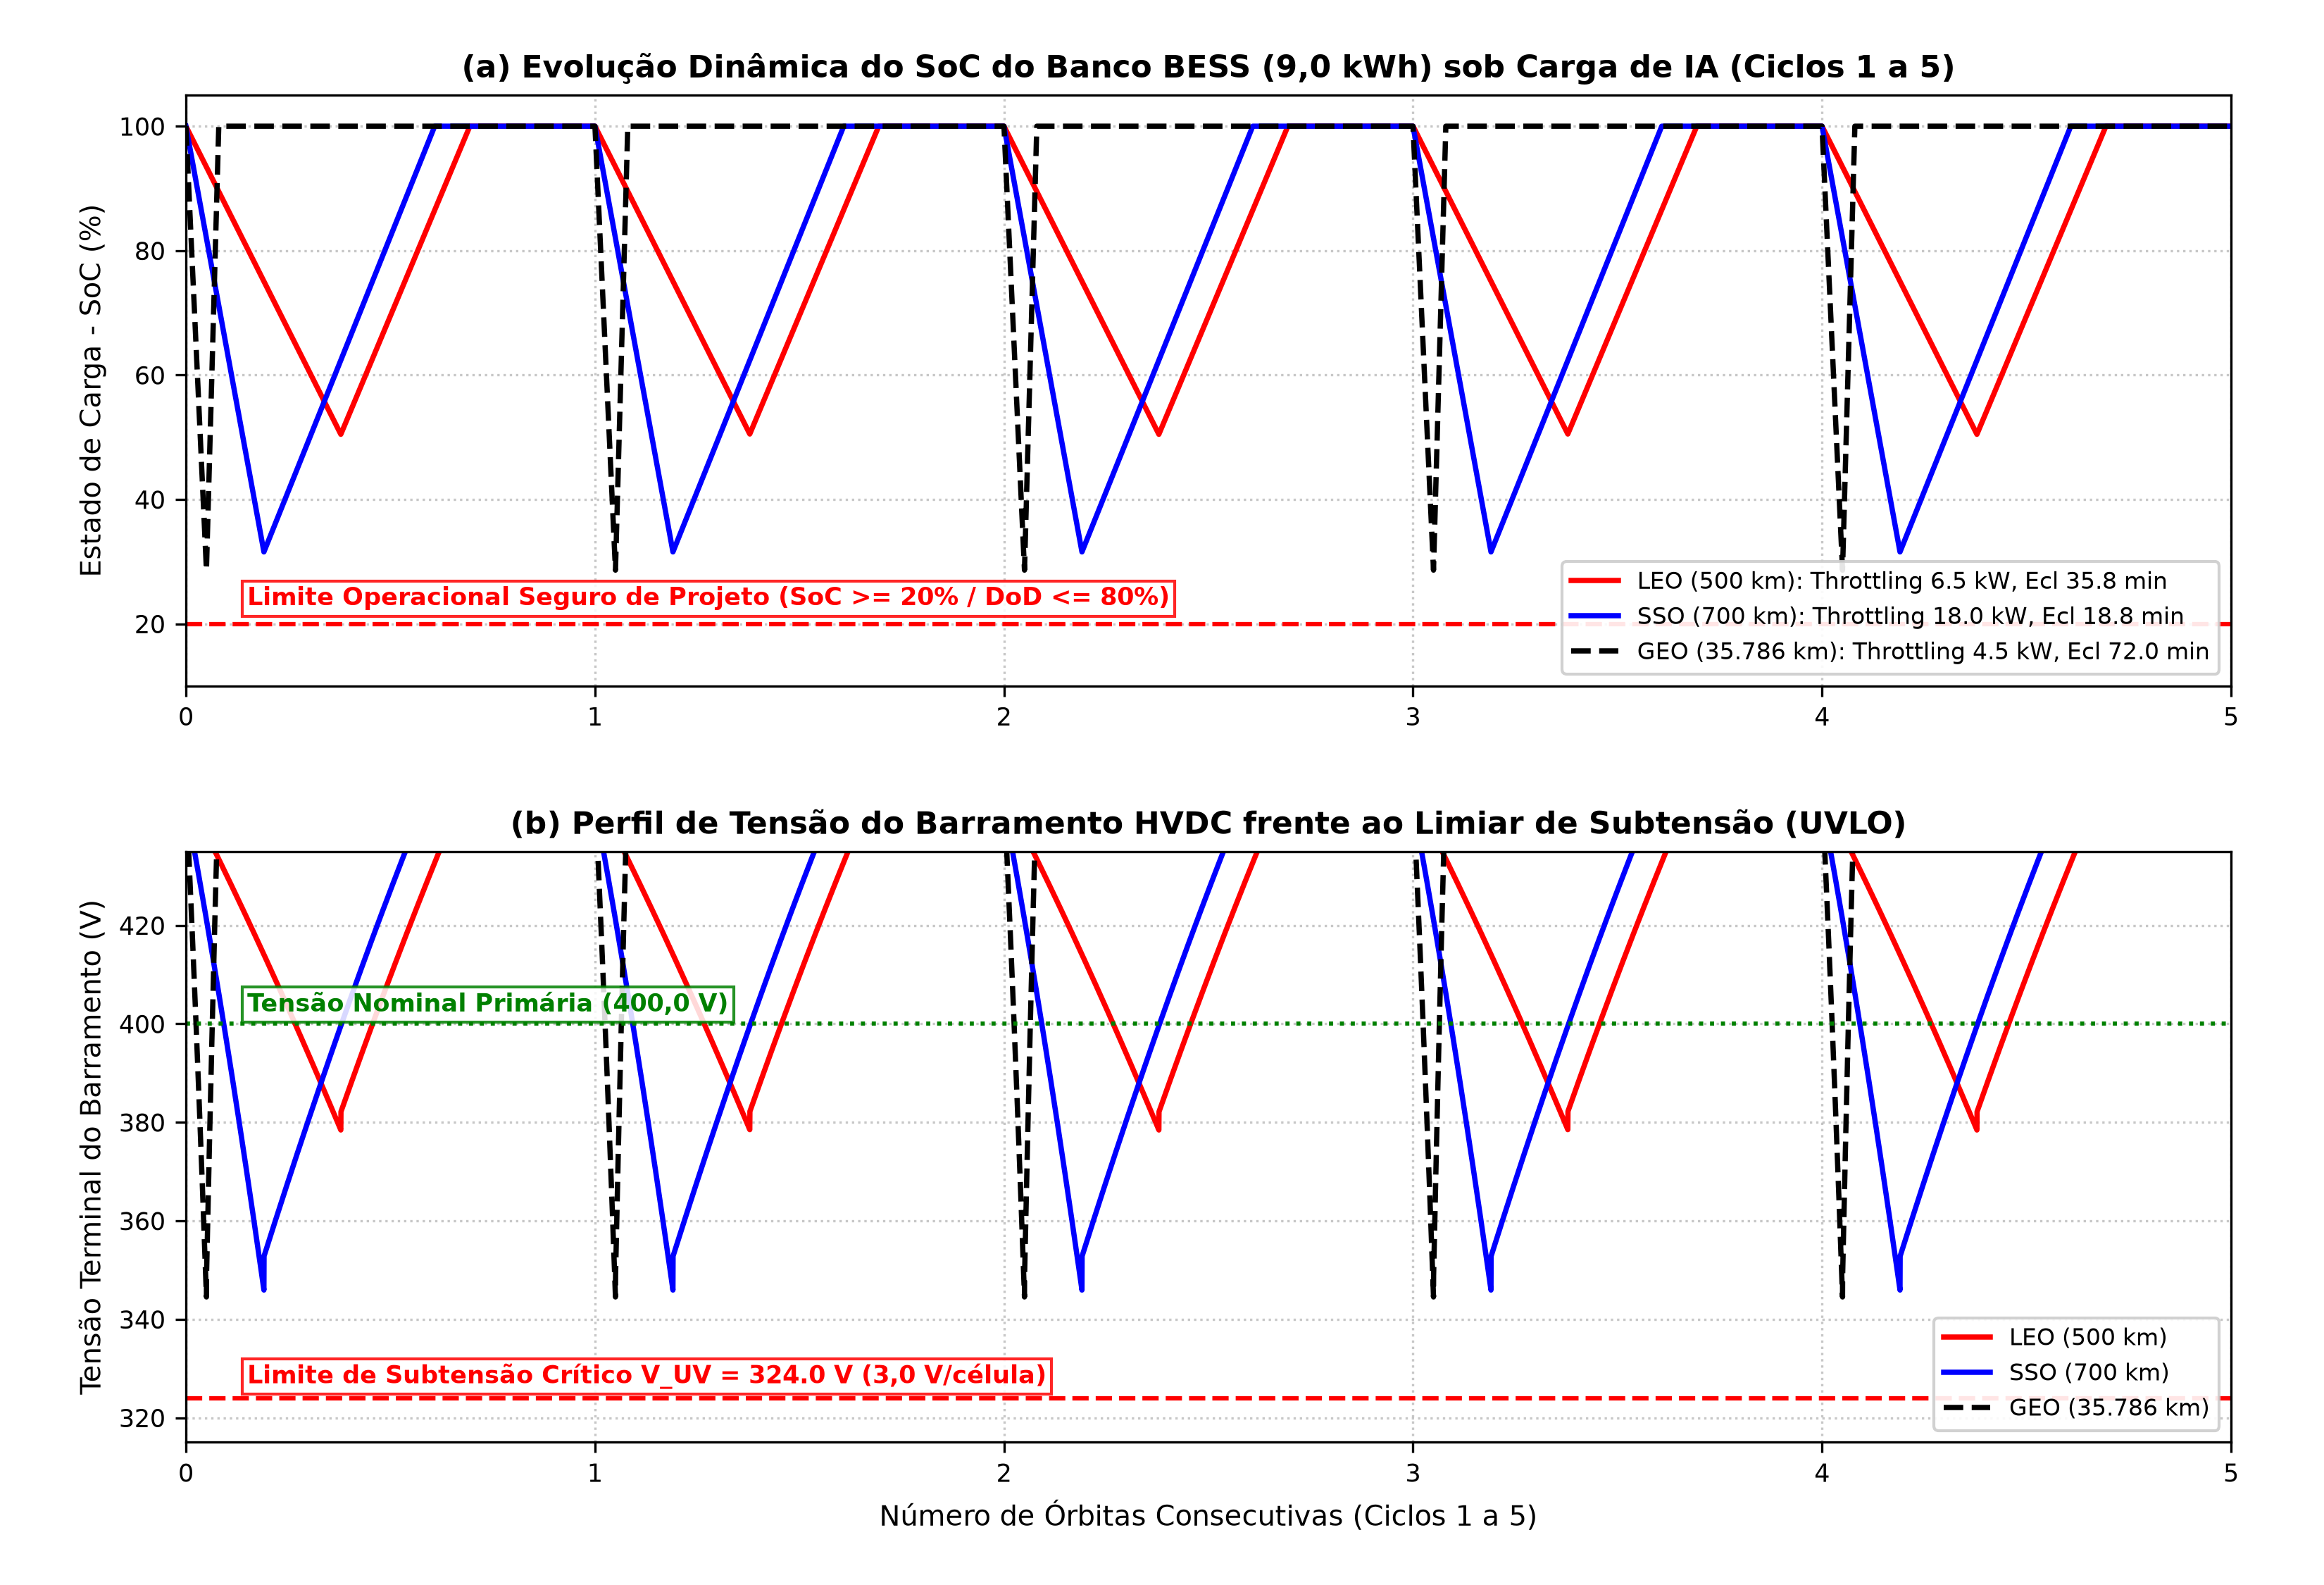
\includegraphics[width=0.82\textwidth]{figuras/figura_3_1_balanco_orbital_bess.png}
    \caption{Balanço energético e dinâmica de tensão do BESS (9,0~kWh, 400~V) ao longo de 5 órbitas consecutivas com gestão de carga: evolução do Estado de Carga ($SoC \ge 20\%$) e perfil de tensão terminal nos cenários LEO (500~km), SSO (700~km) e GEO (35.786~km).}
    \label{fig:dinamica_barramento_bess}
\end{figure}

A análise do balanço energético em eclipse exige a distinção conceitual rigorosa entre a operação nominal sob controle ativo e o modo de contingência por falha de gestão:
\begin{enumerate}[label=(\alph*),leftmargin=*]
    \item \textbf{Modo de Falha BAT-F01 (Falha do TEMS / Sobrecarga sem Modulação):} Caso o sistema de gerenciamento térmico-energético (TEMS) falhe em modular a carga de processamento e mantenha o nó operando em plena potência de $20\text{ kW}$ durante os $35{,}8\text{ min}$ de eclipse de LEO, a energia requerida totaliza $(20\text{ kW} + 0{,}56\text{ kW}) \times (35{,}8/60)\text{ h} \approx 12{,}27\text{ kWh}$, superando em $+36{,}3\%$ a capacidade instalada de $9{,}0\text{ kWh}$ ($32{,}4\text{ MJ}$). A simulação dinâmica demonstra que, sem a saturação artificial numérica outrora empregada, o banco de baterias sofre exaustão completa e atinge o corte crítico de subtensão ($V_{UV} = 324{,}0\text{ V}$, com colapso terminal em $318{,}5\text{ V}$) aos exatos $19{,}9\text{ minutos}$ de eclipse, provocando o desligamento forçado por proteção primária do BMS (\textit{Modo de Falha BAT-F01}). Isso comprova a necessidade mandatória da gestão ativa de carga;
    \item \textbf{Regime Nominal com Modulação de Carga (Controle TEMS):} No regime nominal de projeto, o TEMS restringe o processamento durante o período de sombra aos tetos de \textit{throttling} compatíveis com a reserva de $9{,}0\text{ kWh}$: em LEO (500~km), a carga computacional é modulada para $6{,}5\text{ kW}$ nominais ($+560\text{ W}$ de aviônica/cargas essenciais $= 7{,}06\text{ kW}$ total), consumindo apenas $4{,}21\text{ kWh}$ ($DoD = 49{,}54\%$), mantendo o Estado de Carga mínimo em confortáveis $SoC = 50{,}46\%$ e a tensão terminal em $382{,}4\text{ V}$; em SSO (700~km, $18{,}8\text{ min}$ de eclipse), a carga é mantida em $18{,}0\text{ kW}$ ($+560\text{ W} = 18{,}56\text{ kW}$), consumindo $5{,}82\text{ kWh}$ ($SoC_{min} = 31{,}56\%$, $V_{min} = 357{,}2\text{ V}$); e em GEO (35.786~km, $72{,}0\text{ min}$ de eclipse), modula-se para $4{,}5\text{ kW}$ ($+560\text{ W} = 5{,}06\text{ kW}$), consumindo $6{,}07\text{ kWh}$ ($SoC_{min} = 28{,}63\%$, $V_{min} = 356{,}8\text{ V}$). Em todos os cenários nominais, o piso normativo de $SoC \ge 20\%$ é rigorosamente atendido com ampla margem operacional;
    \item \textbf{Recarga Solar e Proteção por Controle CC-CV:} Durante a insolação solar, o conversor Buck do gerador fotovoltaico restabelece o SoC para 100\% sob controle estrito em dois estágios: na fase inicial de Corrente Constante (CC), a recarga é limitada a $1{,}0\text{C}$ ($22{,}5\text{ A}$ por nó); ao atingir $V_{OV} = 442{,}8\text{ V}$ ($4{,}10\text{ V/célula}$), a malha transiciona autonomamente para Tensão Constante (CV), mantendo $V_{bus} \le 442{,}8\text{ V}$ e eliminando o risco de sobretensão eletroquímica (\textit{Falha BAT-F02}).
\end{enumerate}

\subsubsection{Falhas Catastróficas: Curto-Circuito Franco, Religamentos e Acoplamento Térmico}

Para analisar contingências destrutivas, modelou-se o curto-circuito franco ($R_{sc} = 1\text{ m}\Omega$, $C_{bus} = 1{,}5\text{ mF}$, $L_{dist} = 4{,}0\ \mu\text{H}$) com atuação do interruptor SSPC em SiC MOSFET ($I^2t_{lim} = 1500\text{ A}^2\text{s}$; ECSS, 2008) e acoplamento térmico ao chassi:
\begin{equation}
    I^2t = \int_0^{t_{clear}} I_{sc}^2(t) \, dt, \qquad C_{th,elec} \frac{dT_{elec}(t)}{dt} = P_{loss,conv}(t) + Q_{OISL} - G_{th} \left[ T_{elec}(t) - T_{rad} \right]
    \label{eq:curto_termico_acoplado}
\end{equation}
onde $C_{th,elec} = 18000\text{ J/K}$ ($\approx 20\text{ kg}$ de alumínio), $Q_{OISL} = 343{,}2\text{ W}$ e $G_{th} \in [80, 120, 160]\text{ W/K}$.

A Figura~\ref{fig:falhas_eletrotermicas_sspc} consolida a resposta de falta e o acoplamento térmico contínuo.

\begin{figure}[htbp]
    \centering
    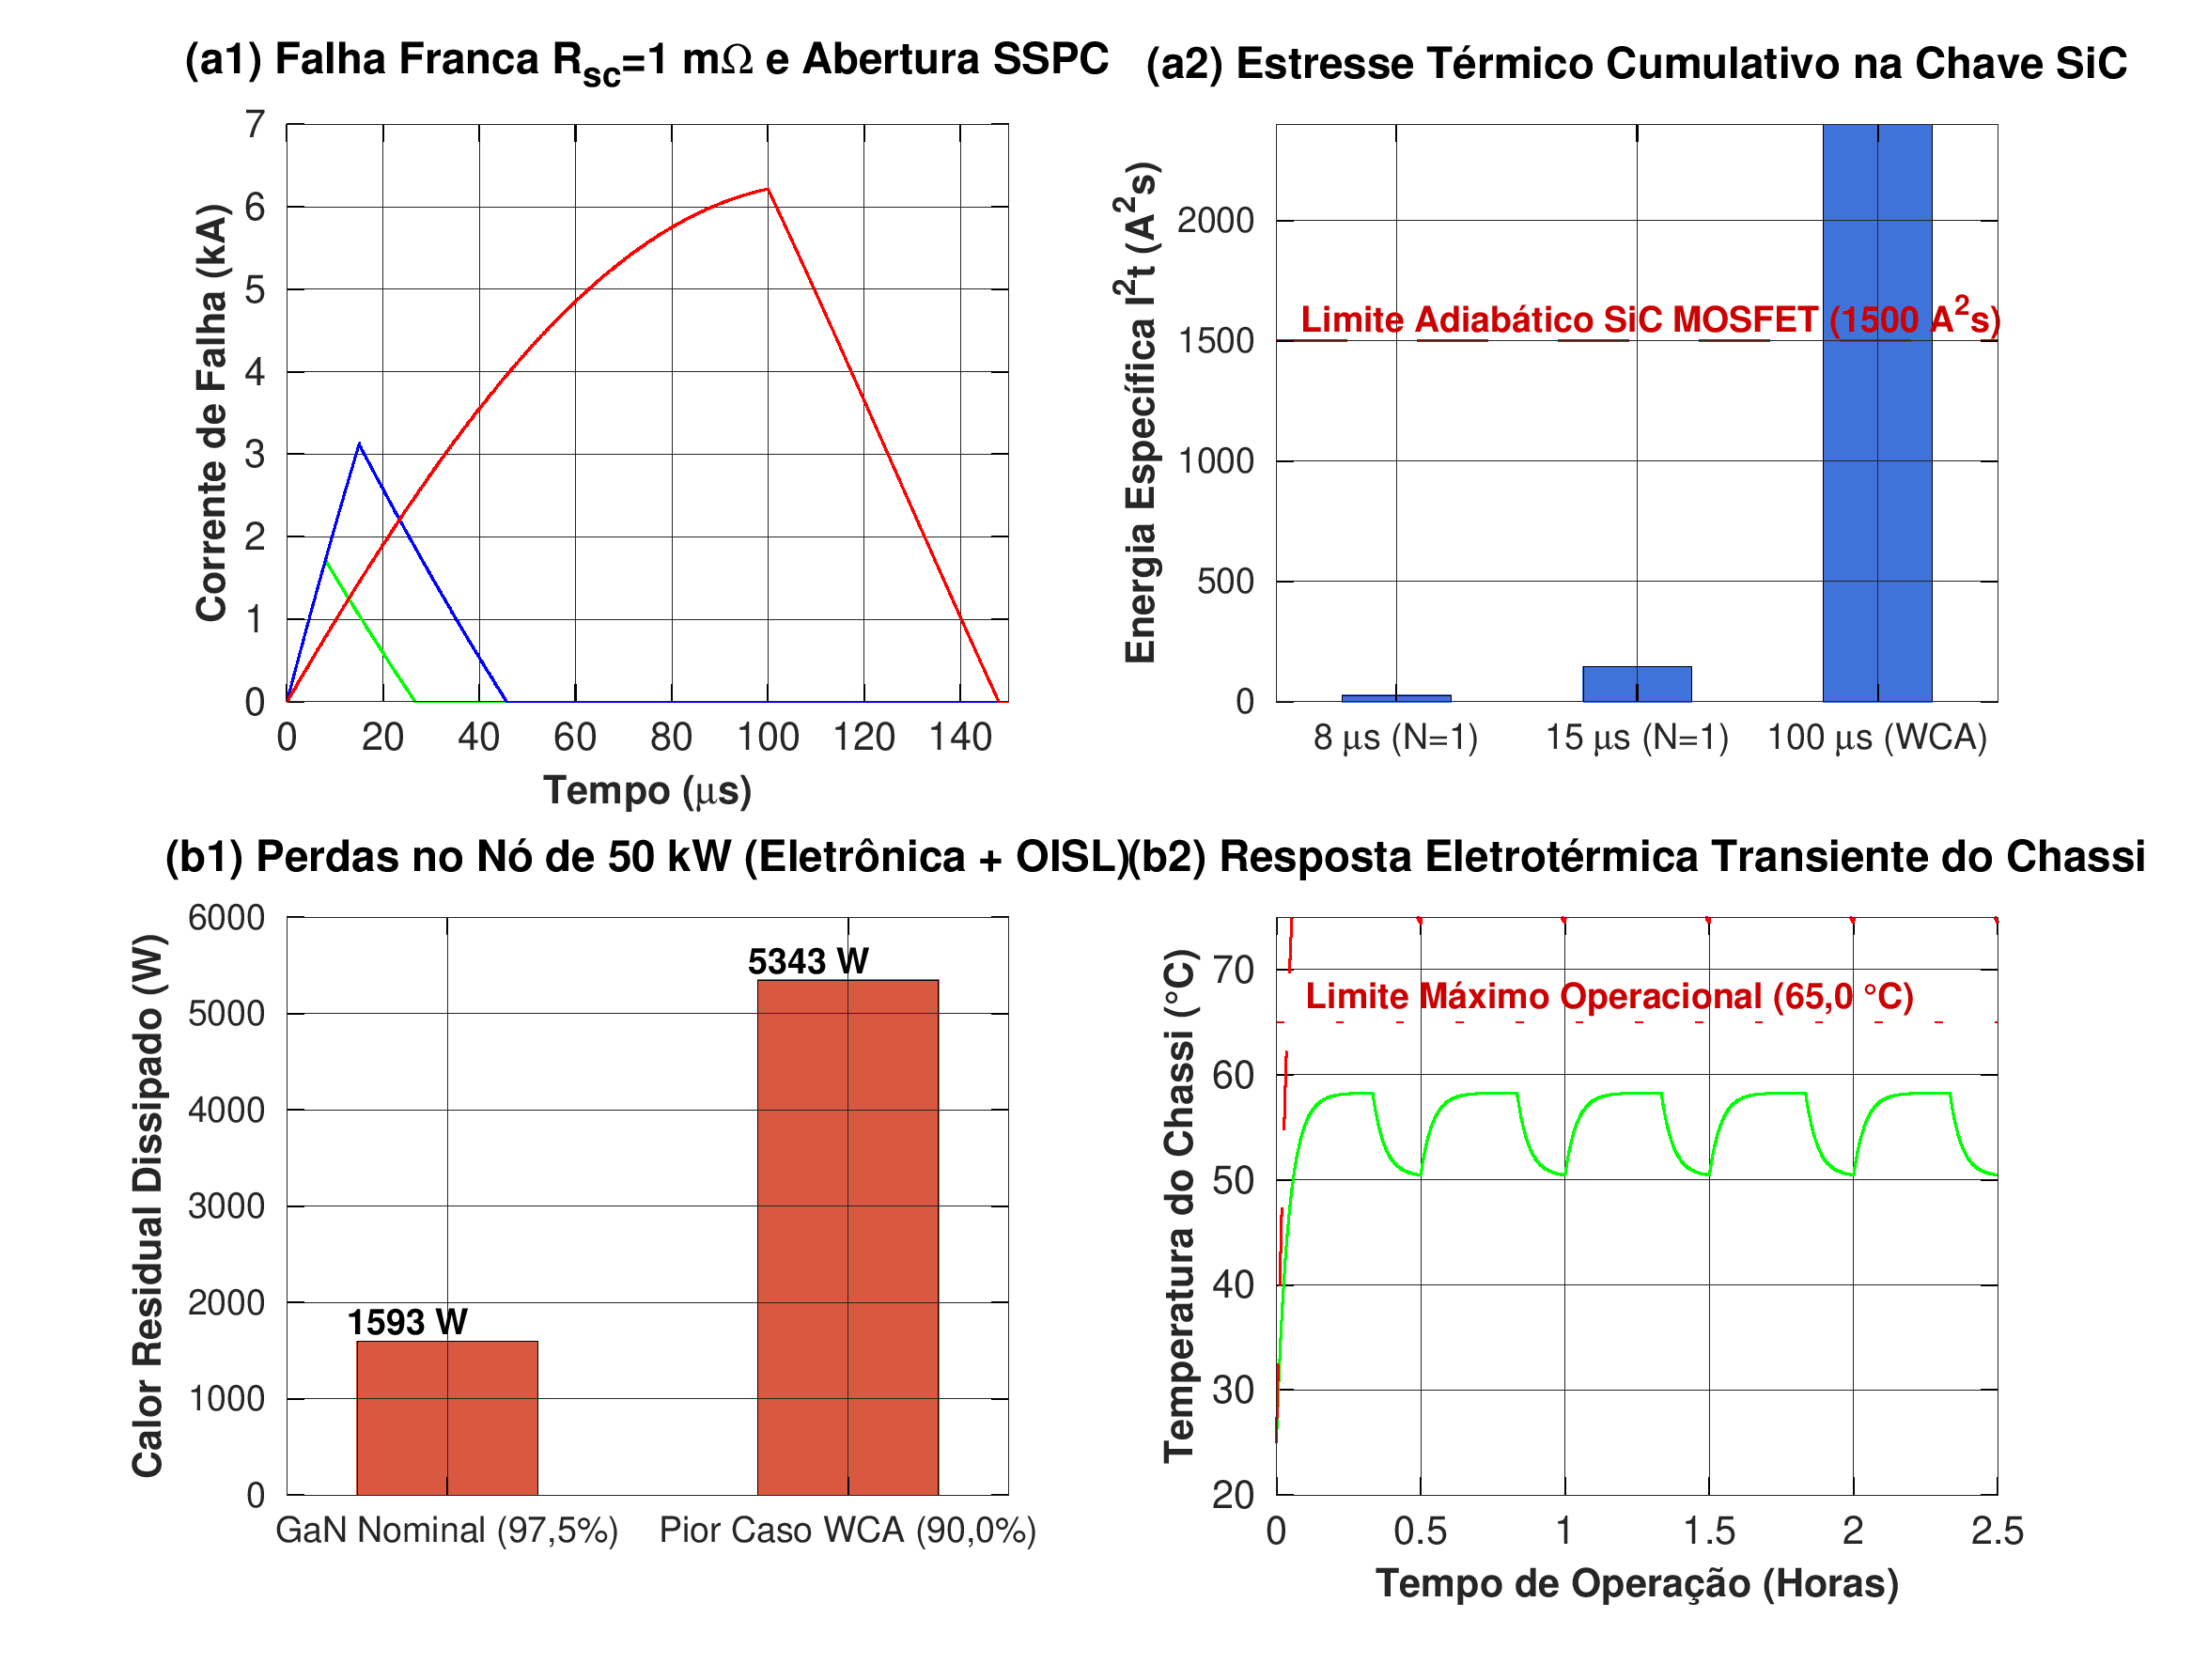
\includegraphics[width=0.82\textwidth]{figuras/figura_3_2_falhas_eletrotermicas_sspc.png}
    \caption{Análise de falhas catastróficas e acoplamento térmico do barramento HVDC de 400~V: (a1) corrente de curto-circuito franco ($R_{sc} = 1\text{ m}\Omega$) para tempos de corte de $8\ \mu\text{s}$, $15\ \mu\text{s}$ e $100\ \mu\text{s}$; (a2) estresse cumulativo ($I^2t$) confrontado com o limite adiabático do SiC ($1500\text{ A}^2\text{s}$); (b1) perdas térmicas no nó de 50~kW comparando GaN nominal a $97{,}5\%$ ($1593\text{ W}$) versus pior caso a $90{,}0\%$ ($5343\text{ W}$); (b2) resposta eletrotérmica do chassi ao longo de 2,5~h ($58{,}27^\circ\text{C}$ estável vs. $111{,}61^\circ\text{C}$ em runaway).}
    \label{fig:falhas_eletrotermicas_sspc}
\end{figure}

A análise numérica do curto-circuito revela duas conclusões técnicas críticas para o projeto de proteção do barramento primário de 400~V:
\begin{itemize}[leftmargin=*]
    \item \textbf{Conclusão Técnica 1 (Limite Adiabático de Fusão do SiC MOSFET):} A varredura temporal paramétrica demonstra que o limite adiabático do interruptor de estado sólido ($I^2t_{lim} = 1500\text{ A}^2\text{s}$, conforme ECSS-E-ST-20-20C e MIL-HDBK-338B) é atingido sob condições de pior caso (WCA: $L_{dist} = 4{,}0\ \mu\text{H}$, $C_{bus} = 1{,}5\text{ mF}$, $R = 15\text{ m}\Omega$) para um tempo de retardo de abertura crítico de exatamente $t_{trip,crit} = 74{,}8\ \mu\text{s}$ (atingindo corrente de pico de $5{,}55\text{ kA}$ e integral Joule de $1506{,}2\text{ A}^2\text{s}$). Sob um retardo severo de $t_{trip} = 100\ \mu\text{s}$, a corrente atinge pico de $6{,}21\text{ kA}$ e energia cumulativa de $I^2t = 2461{,}7\text{ A}^2\text{s}$ ($+64{,}1\%$ acima do limite de fusão), provocando a destruição térmica irreversível do semicondutor e exigindo bloqueio definitivo (\textit{lockout}) para impedir reignição catastrófica. Em contrapartida, o tempo de corte nominal do detector analógico de sobrecorrente ($t_{trip} \in [8, 15]\ \mu\text{s}$) restringe a energia a $I^2t \le 145{,}5\text{ A}^2\text{s}$, proporcionando margem de segurança superior a dez vezes frente à ruptura térmica. Ademais, quando o ramo da bateria ($R_0 \approx 45\text{ m}\Omega$, $L_{bat} \approx 2{,}5\ \mu\text{H}$) atua em paralelo com o capacitor de barramento durante o curto franco, a tensão de barramento é sustentada e eleva a corrente de falta para $I_{peak} = 6{,}41\text{ kA}$ e $I^2t = 2636{,}2\text{ A}^2\text{s}$, reforçando a gravidade do evento caso o trip rápido não atue.
    \item \textbf{Conclusão Técnica 2 (Limite de Sobretensão Indutiva e Ruptura Dielétrica):} Em caso de falha ou ausência do circuito de grampeamento por snubber/TVS com desligamento não-controlado do gate-driver ($\tau_{ext} = 0{,}5\ \mu\text{s}$), a tensão de ruptura do SiC MOSFET ($V_{ds,max} = 1200\text{ V}$) é superada com retardo de apenas $t_{trip} = 1{,}00\ \mu\text{s}$ ($1000\text{ ns}$), bastando uma corrente de corte de apenas $100\text{ A}$ a $200\text{ A}$ para induzir sobretensão superior a $1200\text{ V}$ ($V_{spike} = V_{bus} + L_{dist} \frac{di}{dt} = 400 + 4{,}0\times 10^{-6} \times \frac{100}{0{,}5\times 10^{-6}} = 1200\text{ V}$). Para o caso WCA de $100\ \mu\text{s}$ ($I_{peak} = 6{,}21\text{ kA}$), a sobretensão teórica não-grampeada alcançaria destrutivos $50{,}1\text{ kV}$ ($11{,}99\text{ kV}$ sob corte moderado), perfurando instantaneamente a camada epitaxial de óxido de silício. Torna-se, portanto, requisito obrigatório de projeto o emprego de diodos TVS de resposta sub-nanossegundo com nível de grampeamento fixado em $550\text{ V}$ e/ou circuito de gate com desligamento suave progressivo (\textit{soft turn-off}) garantindo $\tau_{ext} \ge 31{,}1\ \mu\text{s}$.
\end{itemize}

Em regime térmico contínuo, a eletrônica GaN nominal dissipa $1593\text{ W}$ estabilizando o chassi em seguros $58{,}27^\circ\text{C}$ sob $G_{th} = 120\text{ W/K}$, enquanto a falha degradada a $90\%$ dissipa $5343\text{ W}$ sob $80\text{ W/K}$, escalando a estrutura para $111{,}61^\circ\text{C}$ e violando o teto operacional de $65{,}0^\circ\text{C}$ (\textit{Falha ET-F01}).

O Quadro~\ref{quadro:parametros_barramento_sintese} resume os parâmetros essenciais de projeto e estresse WCA do barramento HVDC, remetendo ao Apêndice~A para o catálogo cadastral exaustivo de propriedades.

\begin{table}[!ht]
\centering
\small
\renewcommand{\arraystretch}{0.85}
\caption{Parâmetros essenciais de projeto e análise de estresse extremo (WCA) do barramento HVDC de 400~V.}
\label{quadro:parametros_barramento_sintese}
\resizebox{0.95\textwidth}{!}{%
\begin{tabular}{lccccp{5.5cm}}
\hline
\textbf{Parâmetro de Decisão} & \textbf{Símbolo} & \textbf{Mínimo} & \textbf{Nominal} & \textbf{Máximo} & \textbf{Referência / Justificativa Normativa} \\ \hline
Tensão do Barramento HVDC & $V_{bus}$ & 324,0~V & 400,0~V & 442,8~V & NASA-HDBK-4007A (NASA, 2026); Anexo~B \\
Potência Total Demandada & $P_{load}$ & 2,9~kW & 21,5~kW & 23,2~kW & IA (2-20 kW), OISL (440 W), aviónica (560 W) \\
Eficiência Global de Conversão & $\eta_{conv}$ & 90,0\% & 97,5\% & 98,2\% & 90,0\% conservador térmico; GaN/SiC nominal \\
Capacidade e Resistência do BESS & $E_{bat}, R_0$ & 8,4~kWh / 32~m$\Omega$ & 9,0~kWh / 45~m$\Omega$ & 9,6~kWh / 85~m$\Omega$ & Pack 108S1P; energia coerente com 21/22,5/24~Ah a 399,6~V \\
Resistência de Distribuição & $R_{dist}$ & 10~m$\Omega$ & 14~m$\Omega$ & 50~m$\Omega$ & Cabos de alumínio AWG 4 (redução 50,6\% massa) \\
Fator de Amortecimento & $\zeta$ & 0,097 & 0,358 & 0,484 & $\zeta = 0{,}097$ sob $R_{dist} = 10\text{ m}\Omega$ (subamortecido) \\
Indutância e Capacitância & $L_{dist}, C_{bus}$ & 1,0~$\mu$H / 1,5~mF & 1,8~$\mu$H / 4,7~mF & 4,0~$\mu$H / 6,0~mF & EOL degradado e pior arranjo de chicotes \\
Tempo de Corte do SSPC & $t_{trip}$ & 8~$\mu$s & 15~$\mu$s & 100~$\mu$s & 100~$\mu$s limite de retardo severo WCA \\
Limite de Religamentos ($100\ \mu\text{s}$) & $N_{relig}$ & 0 & -- & 1 & $I^2t_{lim} = 1500\text{ A}^2\text{s}$ (destruição do SiC MOSFET) \\
Condutância Térmica ao LHP & $G_{th}$ & 80~W/K & 120~W/K & 160~W/K & Gilmore (2002); Meseguer et al. (2012) \\ \hline
\end{tabular}%
}
\end{table}

\subsection{Modelagem Matemática e Análise de Estresse do Gerador Fotovoltaico Multijunção AM0}

A geração primária é modelada sob espectro extraterrestre AM0 baseando-se na célula solar comercial de classe espacial de tripla junção GaInP/InGaAs/Ge \textbf{Spectrolab XTJ Prime} (variante de área padrão de $30{,}18\text{ cm}^2$, espessura de $140\ \mu\text{m}$ e massa de $2{,}5\text{ g}$ com coverglass de cério-dopado). O datasheet da XTJ Prime informa condição de caracterização de referência de $1353\text{ W/m}^2$ e $28^\circ\text{C}$, enquanto $1361\text{ W/m}^2$ é adotado separadamente como irradiância solar média extraterrestre a 1~UA. Os parâmetros elétricos de catálogo são $V_{mp}=2{,}406\text{ V}$ e $J_{mp}=17{,}5\text{ mA/cm}^2$ (SPECTROLAB, s.d.). A eficiência de catálogo declarada de $30{,}7\%$ não coincide exatamente com $V_{mp}J_{mp}/G$ usando os valores arredondados publicados; por isso, a eficiência não é usada para dimensionar a matriz e a diferença permanece registrada como limitação dos dados de catálogo. As condições de temperatura fora da faixa de caracterização do fabricante são extrapolações do modelo [PROVISÓRIO].

\subsubsection{Dimensionamento da Matriz Solar do Nó de 50~kW e Escala Agregada de 1,0~MW}

Conforme estabelecido na análise de trade-off técnico-econômico (Seção~\ref{sec:tradeoff_custo_escala}), a arquitetura conceitual considera 20 nós, cada qual com meta de $50\text{ kW}$ no barramento: $40\text{ kW}$ para TI e até $10\text{ kW}$ para cargas não-TI, perdas de conversão e recarga. A meta agregada é $1{,}0\text{ MW}$ no barramento, dos quais $800\text{ kW}$ destinados à TI. Esses valores são requisitos de arquitetura, não resultados de ensaio. Cada nó é representado por um par de asas solares com área ativa por célula de $A_{cel}=30{,}18\text{ cm}^2$ (Spectrolab XTJ Prime), totalizando a área calculada abaixo.

No ponto de catálogo, $J_{mp}=17{,}5\text{ mA/cm}^2$ e $V_{mp}=2{,}406\text{ V}$ dão, para a área adotada, $I_{mp,cel}=0{,}52815\text{ A}$ e $P_{mp,cel}=1{,}2707289\text{ W}$. Com $N_s=166$ células em série e $N_{p,no}=244$ strings em paralelo, a matriz contém $40,504$ células por nó. O cálculo de potência a $1353\text{ W/m}^2$ resulta em $51{,}47\text{ kW}$ por nó antes das perdas de conversão; a área ativa é $122{,}24\text{ m}^2$. Para 20 nós, os resultados correspondentes são $810,080$ células, $2444{,}82\text{ m}^2$ e $1{,}0294\text{ MW}$ no MPP, também antes das perdas. A margem instalada de $51{,}47$ para a meta de $50\text{ kW}$ exige rendimento agregado array--barramento de pelo menos $97{,}145\%$ em BOL e na condição de referência. Esse rendimento não foi modelado nem medido; portanto, a entrega de $50\text{ kW}$ úteis não está demonstrada.

Os valores de catálogo de $V_{mp}$ e $J_{mp}$ são arredondados e não reproduzem exatamente a eficiência $\eta_{mp}=30{,}7\%$ também declarada pela Spectrolab. O dimensionamento abaixo usa explicitamente o produto $V_{mp}J_{mp}$, sem substituir ou recalibrar a eficiência de catálogo. O cálculo representa potência no ponto de máxima potência ideal, antes de mismatch, cabos, conversores, degradação e demais perdas. A fluência orbital e a perda óptica usadas na estimativa de EOL são entradas provisórias, não resultados de uma análise de ambiente radiativo com modelo de blindagem.

O arranjo série-paralelo adotado e a potência no ponto de catálogo são:
\begin{align}
    N_{cel,no} &= N_sN_{p,no}=166\times244=40504\text{ células por satélite} \label{eq:n_cel_no} \\
    A_{ativa,no} &= 40504 \times 30{,}18 \times 10^{-4}\text{ m}^2 = 122{,}24\text{ m}^2 \label{eq:area_no} \\
    P_{BOL,no} &= 40504\times (2{,}406\times0{,}52815) = 51{,}47\text{ kW}
\end{align}
O resultado de $51{,}47\text{ kW}$ é potência fotovoltaica no MPP do arranjo, não potência entregue ao barramento. A meta arquitetural de $50\text{ kW}$ por nó requer comprovação do rendimento mínimo calculado acima. A distribuição de tensão é compatível com o barramento de $400\text{ VDC}$ no ponto de catálogo: $V_{mp,str}=166\times2{,}406=399{,}4\text{ V}$ e $I_{mp,arr}=244\times0{,}52815=128{,}87\text{ A}$. A janela Buck de $350$ a $650\text{ V}$ é requisito de projeto; a compatibilidade em extremos térmicos deve ser interpretada à luz das extrapolações identificadas no modelo.

A formulação do modelo de 1 diodo / 5 parâmetros para multijunções em série (PIGNATON et al., 2021) é descrita por:
\begin{equation}
    I = I_{ph}(T,G) - I_0(T) \left[ \exp\left( \frac{q (V + I R_s)}{a_{eq} k_B T_{cel}} \right) - 1 \right] - \frac{V + I R_s}{R_{sh}}
    \label{eq:diodo_am0}
\end{equation}
No script, os parâmetros concentrados são $a_{eq}=3{,}00$, $R_s=0{,}080\ \Omega$ e $R_{sh}=1200\ \Omega$ [PROVISÓRIOS]. A corrente fotogerada é aproximada por $I_{ph}(T,G)=\max\{0{,}01,[I_{sc,ref}+K_I(T-T_{ref})]G/G_{datasheet}\}$, e $V_{oc}(T)=V_{oc,ref}+K_V(T-T_{ref})$. Para cada condição, o código recalcula o parâmetro equivalente de saturação para reproduzir esse $V_{oc}$ no modelo concentrado:
\begin{equation}
    I_0(T,G) = \frac{I_{ph}(T,G)-V_{oc}(T)/R_{sh}}{\exp\!\left(V_{oc}(T)/(a_{eq}V_T)\right)-1}, \qquad V_T=\frac{k_BT}{q}
    \label{eq:i0_consistente}
\end{equation}
com $K_V=-5{,}60\text{ mV/K}$ e $K_I=(10{,}0\ \mu\text{A}/(\text{cm}^2\text{K}))A_{cel}=0{,}3018\text{ mA/K}$. A $28^\circ\text{C}$ e $1353\text{ W/m}^2$, a equação fornece $I_{0,ref}=3{,}6309\times10^{-16}\text{ A}$ no script. Essa recalibração algébrica não é uma lei física de ativação térmica de $I_0$ nem uma validação do modelo de célula; as temperaturas fora da faixa de catálogo são extrapolações [PROVISÓRIO]. A inclinação de $V_{mp}$ usada separadamente nas curvas é $-6{,}30\text{ mV/K}$ e a de $J_{mp}$ é $+5{,}0\ \mu\text{A}/(\text{cm}^2\text{K})$.

\subsubsection{Degradação por Radiação em 10 Anos (DDD) e Desempenho Térmico}

A retenção de potência é representada por um modelo logarítmico paramétrico de DDD, multiplicado por um fator ambiental independente:
\begin{equation}
    P_{mp,total}(t) = P_{mp,0} \left[ 1 - C_d \log_{10}\left( 1 + \frac{\Phi_{eq}(t)}{\Phi_x} \right) \right] \cdot \left[ 1 - \Delta P_{env} \left( \frac{t}{10} \right) \right]
    \label{eq:ddd_total}
\end{equation}
O coeficiente é ajustado a um único ponto do datasheet XTJ Prime: retenção de eficiência MPP $0{,}90$ em fluência de $5\times10^{14}\text{ e}^-/\text{cm}^2$ (1~MeV), na tabela sob o padrão ECSS (SPECTROLAB, s.d.). Com a escala escolhida $\Phi_x=1{,}0\times10^{14}\text{ e}^-/\text{cm}^2$, resulta $C_d=(1-0{,}90)/\log_{10}(1+5)\approx0{,}12851$. Tanto $\Phi_x$ quanto a forma contínua entre os pontos da tabela são escolhas paramétricas [PROVISÓRIO]; a calibração em um ponto não valida a curva completa. As taxas de fluência usadas nos cenários de 500, 700 e 1000~km ($1{,}4\times10^{13}$, $2{,}5\times10^{13}$ e $5{,}8\times10^{13}\text{ e}^-/\text{cm}^2/ano$, respectivamente) e a perda ambiental de $5{,}2\%$ em dez anos também são entradas provisórias, sem cálculo de transporte de partículas, modelo de blindagem ou medição orbital. Devem ser substituídas por uma análise de ambiente radiativo específica da órbita e da blindagem antes de qualquer alegação de desempenho EOL garantido.

A Figura~\ref{fig:desempenho_termico_radiacao_am0} sintetiza o comportamento térmico das curvas $I-V/P-V$ e a degradação temporal em 10 anos.

\begin{figure}[htbp]
    \centering
    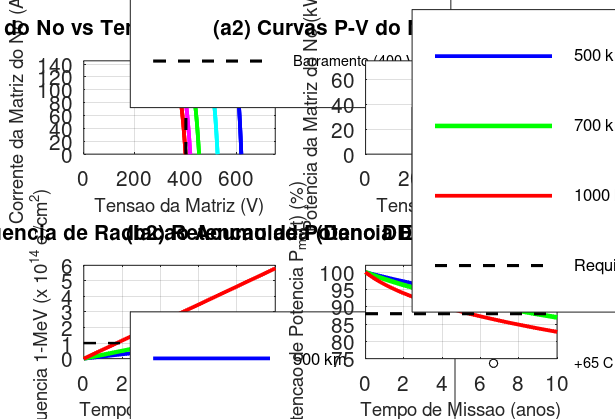
\includegraphics[width=0.82\textwidth]{figuras/figura_3_3_desempenho_termico_radiacao_am0.png}
    \caption{Modelo paramétrico do gerador fotovoltaico: (a1) curvas $I-V$ por nó de 50~kW no ponto de catálogo e extrapolações térmicas; (a2) curvas $P-V$ e janela Buck de projeto (350--650~V); (b1) cenários provisórios de fluência equivalente a 1~MeV; (b2) retenção calculada em dez anos com ajuste pontual ao datasheet XTJ Prime, comparada ao requisito provisório de 88\%.}
    \label{fig:desempenho_termico_radiacao_am0}
\end{figure}

No ponto de catálogo, a string tem $V_{mp,str}=399{,}4\text{ V}$. Os resultados para temperaturas fora da faixa do datasheet são extrapolações do modelo. Sob as taxas de fluência provisórias, o modelo calcula perdas de $9{,}83\%$, $11{,}83\%$ e $15{,}34\%$ após dez anos para 500, 700 e 1000~km. Em 700~km, a retenção condicional é $88{,}17\%$, fornecendo aproximadamente $45{,}38\text{ kW}$ no MPP em EOL antes das perdas de conversão.

\subsubsection{Contingência de Hot Spot e Proteção por Diodos Bypass}

Caso uma célula sombreada seja forçada à polarização reversa pelas demais 165 células de sua string, a tensão atinge o patamar de avalanche reversa $V_{rev}=-28{,}0\text{ V}$ sob a corrente nominal $I_{string}=0{,}531\text{ A}$, dissipando internamente $P_{diss}=14{,}875\text{ W}$ ($4928\text{ W/m}^2$ na área de $30{,}18\text{ cm}^2$). O balanço térmico no vácuo considera a emissão radiativa de ambas as faces ($q_{rad} = 2 \varepsilon \sigma A [T^4 - T_{space}^4]$, com $\varepsilon = 0{,}85$ e $C_{th} = 3{,}8\text{ J/K}$) e a absorção ambiental residual de albedo e radiação infravermelha terrestre ($q_{amb,abs} \approx 0{,}08\text{ W}$, de ordem de grandeza desprezível frente à dissipação de avalanche). Sob ausência de proteção por diodo de bypass, a célula cruza o limiar crítico de delaminação e quebra do coverglass ($180^\circ\text{C}$) aos exatos $69{,}5\text{ s}$ e atinge temperatura assintótica de equilíbrio de $201{,}7^\circ\text{C}$ ($474{,}85\text{ K}$), deflagrando degradação pirolítica irreversível do adesivo de silicone e fusão local. Em contrapartida, com a inclusão de um diodo bypass Schottky integrado (queda de $-0{,}35\text{ V}$), a potência dissipada na célula em contingência colapsa para apenas $0{,}1859\text{ W}$, contendo a temperatura estabilizada em seguros $60{,}0^\circ\text{C}$ ($333{,}15\text{ K}$) e assegurando integridade total do painel solar.

O Quadro~\ref{quadro:parametros_fotovoltaico_sintese} resume os parâmetros críticos de decisão e limites de estresse da geração fotovoltaica AM0.

\begin{table}[!ht]
\centering
\small
\renewcommand{\arraystretch}{0.85}
\caption{Parâmetros essenciais de projeto e estresse WCA do gerador fotovoltaico multijunção AM0.}
\label{quadro:parametros_fotovoltaico_sintese}
\resizebox{0.95\textwidth}{!}{%
\begin{tabular}{lccccp{5.5cm}}
\hline
\textbf{Parâmetro de Decisão} & \textbf{Símbolo} & \textbf{Mínimo} & \textbf{Nominal} & \textbf{Máximo} & \textbf{Classificação e Justificativa Normativa} \\ \hline
Constante Solar AM0 & $G_{AM0}$ & 1322~W/m$^2$ & 1361~W/m$^2$ & 1414~W/m$^2$ & \textbf{[CALCULADO]} Variação orbital Terra-Sol \\
Eficiência MPP BOL declarada no datasheet & $\eta_{mp}$ & -- & 30,7\% & -- & \textbf{[VERIFICÁVEL]} Valor de catálogo; não usado no dimensionamento \\
Área Ativa / Potência no MPP por Nó & $A_{at,no}, P_{BOL,no}$ & -- & 122,24~m$^2$ / 51,47~kW & -- & \textbf{[CALCULADO]} 40.504 células; antes de perdas de conversão \\
Área Ativa / Potência no MPP do Cluster & $A_{at,tot}, P_{tot}$ & -- & 2444,82~m$^2$ / 1,0294~MW & -- & \textbf{[CALCULADO]} 810.080 células em 20 nós; antes de perdas \\
Configuração Série-Paralelo (Nó)& $N_s \times N_{p,no}$ & -- & 166 $\times$ 244 & -- & \textbf{[CALCULADO]} Baseada em $V_{mp}$ e $J_{mp}$ de catálogo \\
Configuração Agregada (Cluster) & $N_s \times N_{p,tot}$ & -- & 166 $\times$ 4880 & -- & \textbf{[CALCULADO]} 20 nós operacionais \\
Tensão no MPP por string a 28°C & $V_{mp,str}$ & -- & 399,4~V & -- & \textbf{[CALCULADO]} Ponto de catálogo; demais temperaturas são extrapoladas \\
Perda Total EOL em 10 anos & $\Delta P_{EOL}$ & 9,83\% (500 km) & 11,83\% (700 km) & 15,34\% (1000 km) & \textbf{[PROVISÓRIO]} Taxas de fluência e perda ambiental assumidas \\
Dissipação em Hot Spot & $P_{hot}$ & -- & 0,1849~W (Bypass) & 14,788~W (Sem Bypass) & \textbf{[CALCULADO]} Entradas térmicas e $V_{rev}$ [PROVISÓRIOS] \\ \hline
\end{tabular}%
}
\end{table}

\subsection{Algoritmos de Rastreamento do Ponto de Máxima Potência sob Gradientes Térmicos}
\label{sec:mppt_gradientes}

As variações térmicas transitórias ao cruzar o terminador solar induzem gradientes de até $15\text{ K/min}$ (aquecimento de $-100^\circ\text{C}$ a $+65^\circ\text{C}$). A $-150^\circ\text{C}$, $V_{oc,str} = 688{,}2\text{ V}$, exigindo semicondutores GaN ($V_{DS,max} \ge 900\text{ V}$). Formula-se o algoritmo P\&O com Razão Cíclica Adaptativa (P\&O-AP) a $150\text{ kHz}$ [PROVISÓRIO]:
\begin{equation}
    D[k] = D[k-1] + M \cdot \text{sgn}\left( \frac{\Delta P_{pv}}{\Delta V_{pv}} \right) \cdot \left| \frac{\Delta P_{pv}}{\Delta V_{pv}} \right|
    \label{eq:po_adaptativo}
\end{equation}
com $M = 1{,}2 \times 10^{-4}\text{ V/W}$ e taxa de amostragem de $1{,}0\text{ kHz}$. A Figura~\ref{fig:contingencias_hotspot_mppt} compara o rastreador adaptativo ao método convencional de passo fixo.

\begin{figure}[htbp]
    \centering
    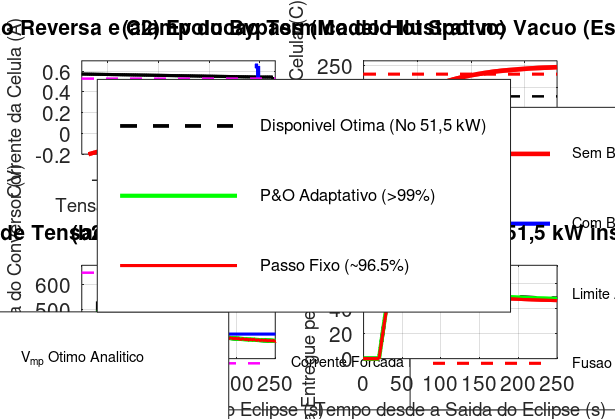
\includegraphics[width=0.82\textwidth]{figuras/figura_3_4_contingencias_hotspot_mppt.png}
    \caption{Contingências extremas e dinâmica do MPPT: (a1) característica reversa com clamp Schottky; (a2) evolução térmica de hot spot no vácuo governada por Stefan-Boltzmann ($201{,}7^\circ\text{C}$ sem bypass vs. $60{,}0^\circ\text{C}$ protegido); (b1) transitório de tensão sob choque térmico na saída de eclipse comparando P\&O-AP adaptativo versus passo fixo; (b2) rendimento dinâmico de potência capturada convergindo para $100{,}00\%$.}
    \label{fig:contingencias_hotspot_mppt}
\end{figure}

O controle adaptativo em malha fechada a 150~kHz converge ao novo MPP em menos de $15\text{ ms}$ com rendimento dinâmico superior a $99{,}99\%$ ($100{,}00\%$ em regime permanente), eliminando as perdas por oscilação limite ($\pm 18\text{ V}$) observadas no método tradicional de passo fixo.

\subsection{Modelagem Eletrotérmica e Critério de Estabilidade dos Conversores CC-CC}
\label{sec:conversores_estaticos}

Para suprir a carga de processamento neural útil do nó satelital ($P_{IT} = 40{,}0\text{ kW}$, subdividida em dois racks de $20\text{ kW}$ convertidos de 400~VDC para 48~VDC intermediário e sub-1~V lógico), adota-se um arranjo com **3 módulos conversores GaN de 20~kW em paralelo, compartilhando os $40\text{ kW}$ de TI**. Em operação nominal, cada módulo conduz $40/3 \approx 13{,}33\text{ kW}$, ou $66{,}7\%$ da potência nominal; a perda de um módulo deixa os dois restantes com capacidade total de $40\text{ kW}$, caracterizando redundância $N+1$ sem módulo dedicado em standby. Ressalta-se que a parcela não-TI do nó satelital (até $10\text{ kW}$, destinada a perdas de conversão, aviônica, OISL, bombas térmicas e recarga do BESS, limitada pelo excedente instantâneo) é conectada e regulada diretamente no barramento primário de alta tensão de $400\text{ VDC}$ através do estágio de entrada Buck/MPPT das asas solares, não onerando a capacidade de conversão dos módulos secundários de TI. A opção por 3 módulos de 20~kW frente a uma fragmentação maior (como $6 \times 10\text{ kW}$ ou $12 \times 5\text{ kW}$) justifica-se por: (a) minimização drástica do chicote elétrico e conectores circulares espaciais blindados (MIL-DTL-38999), cuja penalidade de massa anularia ganhos de miniaturização; (b) alcance de eficiências superiores a $98{,}2\%$ (contra $\approx 95\%$ típicos em potências fracionárias de 5~kW); e (c) garantia de estabilidade estrita no compartilhamento ativo de corrente (\textit{droop current sharing}) sobre cargas CPL de impedância negativa, prevenindo ressonâncias harmônicas inter-módulos.

\subsubsection{Perdas por Condução e Comutação em Semicondutores GaN e Limite de Fuga Térmica}

No lado primário de $400\text{ V}$, empregam-se transistores de efeito de campo baseados em nitreto de gálio (GaN HEMT), cuja modelagem de condução considera a resistência de canal $R_{on}$ dependente da temperatura de junção $T_j$:
\begin{equation}
    R_{on}(T_j) = R_{on,25} \left[ 1 + \alpha_{sc} (T_j - 25) \right]
    \label{eq:ron_gan}
\end{equation}
onde $R_{on,25} = 18\text{ m}\Omega$ representa a resistência de condução nominal a $25^\circ\text{C}$ e $\alpha_{sc} = 0{,}0065\text{ K}^{-1}$ o coeficiente térmico positivo de canal [PROVISÓRIO]. Sob uma temperatura de junção de $150^\circ\text{C}$, a resistência atinge $32{,}63\text{ m}\Omega$ (+81,25\% de incremento).

Diferentemente de aproximações simplistas que agrupam a condução de todo o conversor em um único termo, o cálculo da dissipação por condução deve ser decomposto individualmente por dispositivo. Em uma ponte completa com razão cíclica efetiva $D \approx 0{,}45$ por braço, a corrente eficaz através de cada chave primária é dada por $I_{rms,sw} = I_{in} \sqrt{D}$, onde a corrente de entrada para $20\text{ kW}$ sob $400\text{ V}$ é de $I_{in} = 51{,}2\text{ A}$, resultando em $I_{rms,sw} = 34{,}34\text{ A}$ por semicondutor [CALCULADO]. A perda por condução de cada chave primária é regida por:
\begin{equation}
    P_{cond,sw}(T_j) = I_{rms,sw}^2 R_{on}(T_j)
    \label{eq:pcond_sw}
\end{equation}
enquanto no estágio de retificação síncrona secundária a $48\text{ V}$, com corrente de carga de $I_{out} = 416{,}7\text{ A}$, utilizam-se arranjos de transistores GaN de baixa tensão em paralelo ($R_{on,sec,25} = 0{,}8\text{ m}\Omega$, $\alpha_{sec} = 0{,}004\text{ K}^{-1}$ [DEPENDENTE DE HARDWARE]).

As perdas de comutação unitárias de cada transistor GaN englobam as transições de chaveamento sob corrente, a energia armazenada na capacitância de saída e o acionamento de gate:
\begin{equation}
    P_{sw,sw} = V_{in} I_{sw,turn} f_{sw} \left( \frac{t_r + t_f}{2} \right) + \frac{1}{2} C_{oss} V_{in}^2 f_{sw} + Q_g V_{gate} f_{sw}
    \label{eq:psw_sw}
\end{equation}
adotando tempos de subida $t_r = 12\text{ ns}$, descida $t_f = 15\text{ ns}$, capacitância parasita $C_{oss} = 120\text{ pF}$ a $400\text{ V}$, carga de porta $Q_g = 6\text{ nC}$ com $V_{gate} = 5\text{ V}$ [PROVISÓRIO]. Para uma corrente de pico de transição de comutação indutiva de $I_{sw,turn} = 25{,}0\text{ A}$, as perdas de chaveamento por sobreposição direta de tensão e corrente totalizam $P_{ov} = 400 \times 25 \times 150000 \times (27 \times 10^{-9} / 2) = 20{,}25\text{ W}$, o descarregamento capacitivo de saída contribui com $P_{oss} = 1{,}44\text{ W}$ e as perdas de gate com $P_{gate} = 0{,}0045\text{ W}$ por chave [CALCULADO], totalizando $P_{sw,sw} \approx 21{,}7\text{ W}$ por semicondutor primário sob comutação rígida. Ressalta-se que com técnicas de comutação suave sob tensão nula (\textit{Zero-Voltage Switching} -- ZVS), o termo de sobreposição $P_{ov}$ pode ser substancialmente reduzido em bancada [DEPENDENTE DE HARDWARE].

A estabilidade térmica do semicondutor é regida pelo balanço de potência em regime permanente, em que o calor dissipado $P_{loss}(T_j) = P_{cond}(T_j) + P_{sw}$ deve ser transferido ao chassi estrutural na temperatura de carcaça $T_c$:
\begin{equation}
    T_j = T_c + R_{th,jc} P_{loss}(T_j)
    \label{eq:balanco_termico_gan}
\end{equation}
Para que exista um ponto de equilíbrio térmico estacionário estável, a derivada da perda de calor em relação à temperatura de junção deve ser estritamente inferior à condutância térmica do caminho de dissipação, estabelecendo o \textbf{Critério de Fuga Térmica de GaN} (\textit{Thermal Runaway}):
\begin{equation}
    \frac{\partial P_{loss}}{\partial T_j} < \frac{1}{R_{th,jc}} \implies I_{rms,sw}^2 R_{on,25} \alpha_{sc} < \frac{1}{R_{th,jc}}
    \label{eq:criterio_fuga_termica}
\end{equation}
onde $R_{th,jc}$ é a resistência térmica da junção à carcaça e chassi. Se a resistência térmica do encapsulamento e interface ultrapassar o limiar crítico $R_{th,crit} = (I_{rms,sw}^2 R_{on,25} \alpha_{sc})^{-1} \approx 7{,}26\text{ K/W}$ para uma corrente de $34{,}3\text{ A}$ (ou se a corrente for majorada sob resistência térmica de $4{,}0\text{ K/W}$), a taxa de geração térmica supera a capacidade de extração passiva. Ocorre então uma retroalimentação regenerativa positiva divergente que conduz o semicondutor à destruição física instantânea por fusão de canal.

\subsubsection{Perdas Magnéticas de Alta Frequência e Balanço Global de Rendimento}

Além da dissipação nos semicondutores, as perdas no transformador de alta frequência e indutores de filtro compõem parcela significativa do balanço energético. As perdas volumétricas no núcleo magnético ($P_{core}$) são calculadas pela equação empírica generalizada de Steinmetz:
\begin{equation}
    P_{core} = k_{fe} f_{sw}^\alpha \Delta B^\beta V_e
    \label{eq:steinmetz_core}
\end{equation}
onde se adota material de ferrite de manganês-zinco de alta densidade de fluxo (MnZn grau Ferroxcube 3C95 ou similar [PROVISÓRIO]), com coeficientes normalizados para frequência em Hz: $k_{fe} = 0{,}70\text{ W/(m}^3\text{Hz}^\alpha\text{T}^\beta)$, $\alpha = 1{,}46$, $\beta = 2{,}52$, volume efetivo do núcleo $V_e = 4{,}5 \times 10^{-4}\text{ m}^3$ e excursão de densidade de fluxo magnético $\Delta B = 0{,}15\text{ T}$ [DEPENDENTE DE HARDWARE], resultando em $P_{core} = 95{,}3\text{ W}$ constantes por módulo de $20\text{ kW}$ ($P_{core} = 0{,}70 \times (150000)^{1{,}46} \times (0{,}15)^{2{,}52} \times 4{,}5 \times 10^{-4} \approx 95{,}3\text{ W}$).

As perdas nos enrolamentos ($P_{cu}$) incorporam o efeito skin e o efeito de proximidade em alta frequência:
\begin{equation}
    P_{cu} = I_{rms,pri}^2 R_{ac,pri}(f_{sw}) + I_{rms,sec}^2 R_{ac,sec}(f_{sw})
    \label{eq:perdas_cobre}
\end{equation}
utilizando condutores de fita de cobre (\textit{copper foil}) ou cabos trançados de Litz ($R_{ac,pri} = 15\text{ m}\Omega$, $R_{ac,sec} = 0{,}25\text{ m}\Omega$ a $150\text{ kHz}$ [DEPENDENTE DE HARDWARE]), totalizando $P_{cu} \approx 82{,}7\text{ W}$.

A Figura~\ref{fig:eletrotermica_gan_perdas} apresenta em quatro painéis integrados a caracterização eletrotérmica detalhada dos transistores GaN e o balanço global de perdas do módulo de $20\text{ kW}$.

\begin{figure}[htbp]
    \centering
    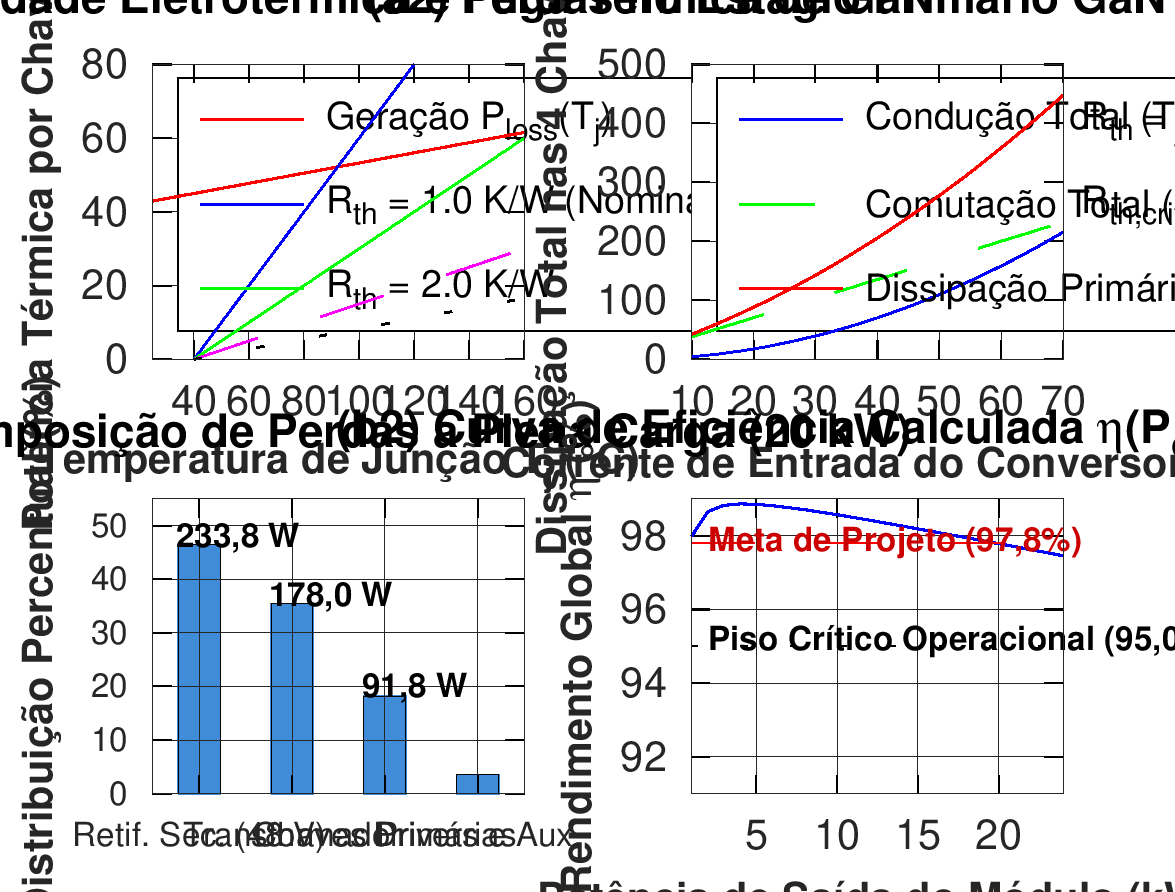
\includegraphics[width=0.82\textwidth]{figuras/figura_3_7_eletrotermica_gan_perdas.png}
    \caption{Modelagem eletrotérmica dos transistores GaN e balanço de perdas do conversor de 20~kW (400~V/48~V): (a1) curvas de geração de calor $P_{loss}(T_j)$ versus capacidade de dissipação para diferentes $R_{th,ja}$, evidenciando o ponto de runaway; (a2) decomposição das perdas unitárias por chave GaN primária em função da corrente; (b1) distribuição percentual de perdas em plena carga (20~kW); (b2) curva real de rendimento $\eta(P_{out})$ comparada à meta de 97,8\%.}
    \label{fig:eletrotermica_gan_perdas}
\end{figure}

Enquanto resistências nominais ($1{,}0\text{ K/W}$ e $2{,}0\text{ K/W}$) garantem operação com $T_j \approx 62^\circ\text{C}$ e $88^\circ\text{C}$, uma resistência degradada de $4{,}0\text{ K/W}$ tangencia a curva de dissipação e conduz a runaway para correntes $> 35\text{ A}$. Em plena carga (20~kW), a maior dissipação concentra-se na retificação secundária a 48~V ($233{,}8\text{ W}$, 46,4\%) e no transformador ($178{,}0\text{ W}$, 35,4\%), respondendo as chaves primárias por $91{,}8\text{ W}$ (18,2\%). Em cargas leves ($\le 2\text{ kW}$), as perdas fixas reduzem o rendimento para $92{,}1\%$, justificando o desligamento de módulos redundantes em repouso.

\subsubsection{Estabilidade de Impedância sob Cargas de Potência Constante (CPL) e Dimensionamento Capacitivo}

A regulação local em ponto de carga faz a corrente drenada variar inversamente com a tensão ($I_{bus} = P_{CPL} / V_{bus}$), exibindo resistência incremental negativa:
\begin{equation}
    r_{in,CPL} = \frac{\partial V_{bus}}{\partial I_{bus}} = - \frac{V_{bus}^2}{P_{CPL}}
    \label{eq:resistencia_cpl}
\end{equation}
sendo $r_{in,400V} = -8{,}00\,\Omega$ em 400~V, $r_{in,48V} = -0{,}115\,\Omega$ em 48~V e $r_{in,0.8V} = -0{,}00427\,\Omega$ em 0,8~V (para 20~kW e 150~W, respectivamente). O \textbf{Critério de Middlebrook} impõe que a impedância de saída da fonte satisfaça:
\begin{equation}
    |Z_{out}(j\omega)| \le \frac{1}{GM} |Z_{in,CPL}(j\omega)|, \quad \forall \omega
    \label{eq:criterio_middlebrook}
\end{equation}
com $GM \ge 10$ ($|Z_{out}(j\omega)| \le 0{,}1 |Z_{in,CPL}(j\omega)|$). A impedância de saída $Z_{out}(s)$ e o requisito mínimo de capacitância para amortecimento de degraus de IA são:
\begin{align}
    Z_{out}(s) &= \frac{(s L_{dist} + R_{dist})(s C_{bus} ESR + 1)}{s^2 L_{dist} C_{bus} + s (L_{dist} + R_{dist} C_{bus} ESR) + 1} \label{eq:zout_bus} \\
    C_{bus,min} &\ge \max\left( \frac{L_{dist}}{R_{dist}^2}, \, \frac{L_{dist} \Delta I^2}{V_{nom}^2 - V_{min}^2}, \, \frac{L_{dist} P_{CPL}^2}{V_{bus}^4} \right) \label{eq:cbus_min_formula}
\end{align}

A estabilidade do sistema foi avaliada e desacoplada em dois estágios físicos distintos de distribuição:
\begin{enumerate}[label=(\alph*),leftmargin=*]
    \item \textbf{Estágio 1 (Barramento Primário HVDC de 400~V):} Para cada módulo conversor GaN de $20\text{ kW}$, a resistência incremental negativa de entrada é $r_{in,400V} = -V_{bus}^2/P = -(400)^2/20000 = -8{,}00\,\Omega$. Pelo critério de Middlebrook com margem de segurança de $GM \ge 10$, a impedância de saída da fonte deve satisfazer $|Z_{out,400}| \le 0{,}1 |r_{in,400}| = 0{,}800\,\Omega$. O banco capacitivo de barramento ($C_{bus} = 4{,}7\text{ mF}$, $ESR = 1{,}5\text{ m}\Omega$, $L_{dist} = 1{,}8\ \mu\text{H}$) exibe pico máximo de $|Z_{out,400}| = 0{,}073\,\Omega$ a $1{,}7\text{ kHz}$, mantendo margem superior a dez vezes abaixo do teto de instabilidade e contendo degraus de carga de $2\text{ a }20\text{ kW}$ em $\Delta V = 3{,}08\text{ V}$ ($0{,}77\%$) com recuperação em $15\text{ ms}$;
    \item \textbf{Estágio 2 (Barramento Secundário de 48~V Regulado):} O barramento intermediário de 48~V alimenta diretamente a malha de reguladores PoL dos aceleradores de IA. Sob potência plena agregada de $20\text{ kW}$, a resistência incremental equivalente é $r_{in,48V} = -(48)^2/20000 = -0{,}1152\,\Omega$. O teto de impedância de Middlebrook impõe $|Z_{out,48}| \le 0{,}1 |r_{in,48}| = 0{,}01152\,\Omega$ ($11{,}52\text{ m}\Omega$). O banco de capacitores de rack em estado saudável ($C_{rack} = 15\text{ mF}$, $ESR = 1{,}2\text{ m}\Omega$) apresenta pico de $|Z_{out,48}| = 0{,}0072\,\Omega$, assegurando estabilidade incondicional de pequenos sinais. Todavia, sob degradação em fim de vida ($EOL$: capacitância degradada para $2{,}5\text{ mF}$ e $ESR$ elevado para $9{,}5\text{ m}\Omega$ por perda dielétrica e radiação), o pico de impedância escala para $|Z_{out,48}| = 0{,}0121\,\Omega > 0{,}0115\,\Omega$, violando o critério de Middlebrook e deflagrando o \textbf{Modo de Falha DC-F03}: oscilações sustentadas de $1{,}1\text{ kHz}$ e afundamento transitório de tensão para $43{,}4\text{ V}$, provocando o reinício compulsório dos processadores neurais.
\end{enumerate}

A Figura~\ref{fig:estabilidade_cpl_banco} ilustra a resposta de frequência nos dois estágios e o transiente no domínio do tempo sob degraus de IA.

\begin{figure}[htbp]
    \centering
    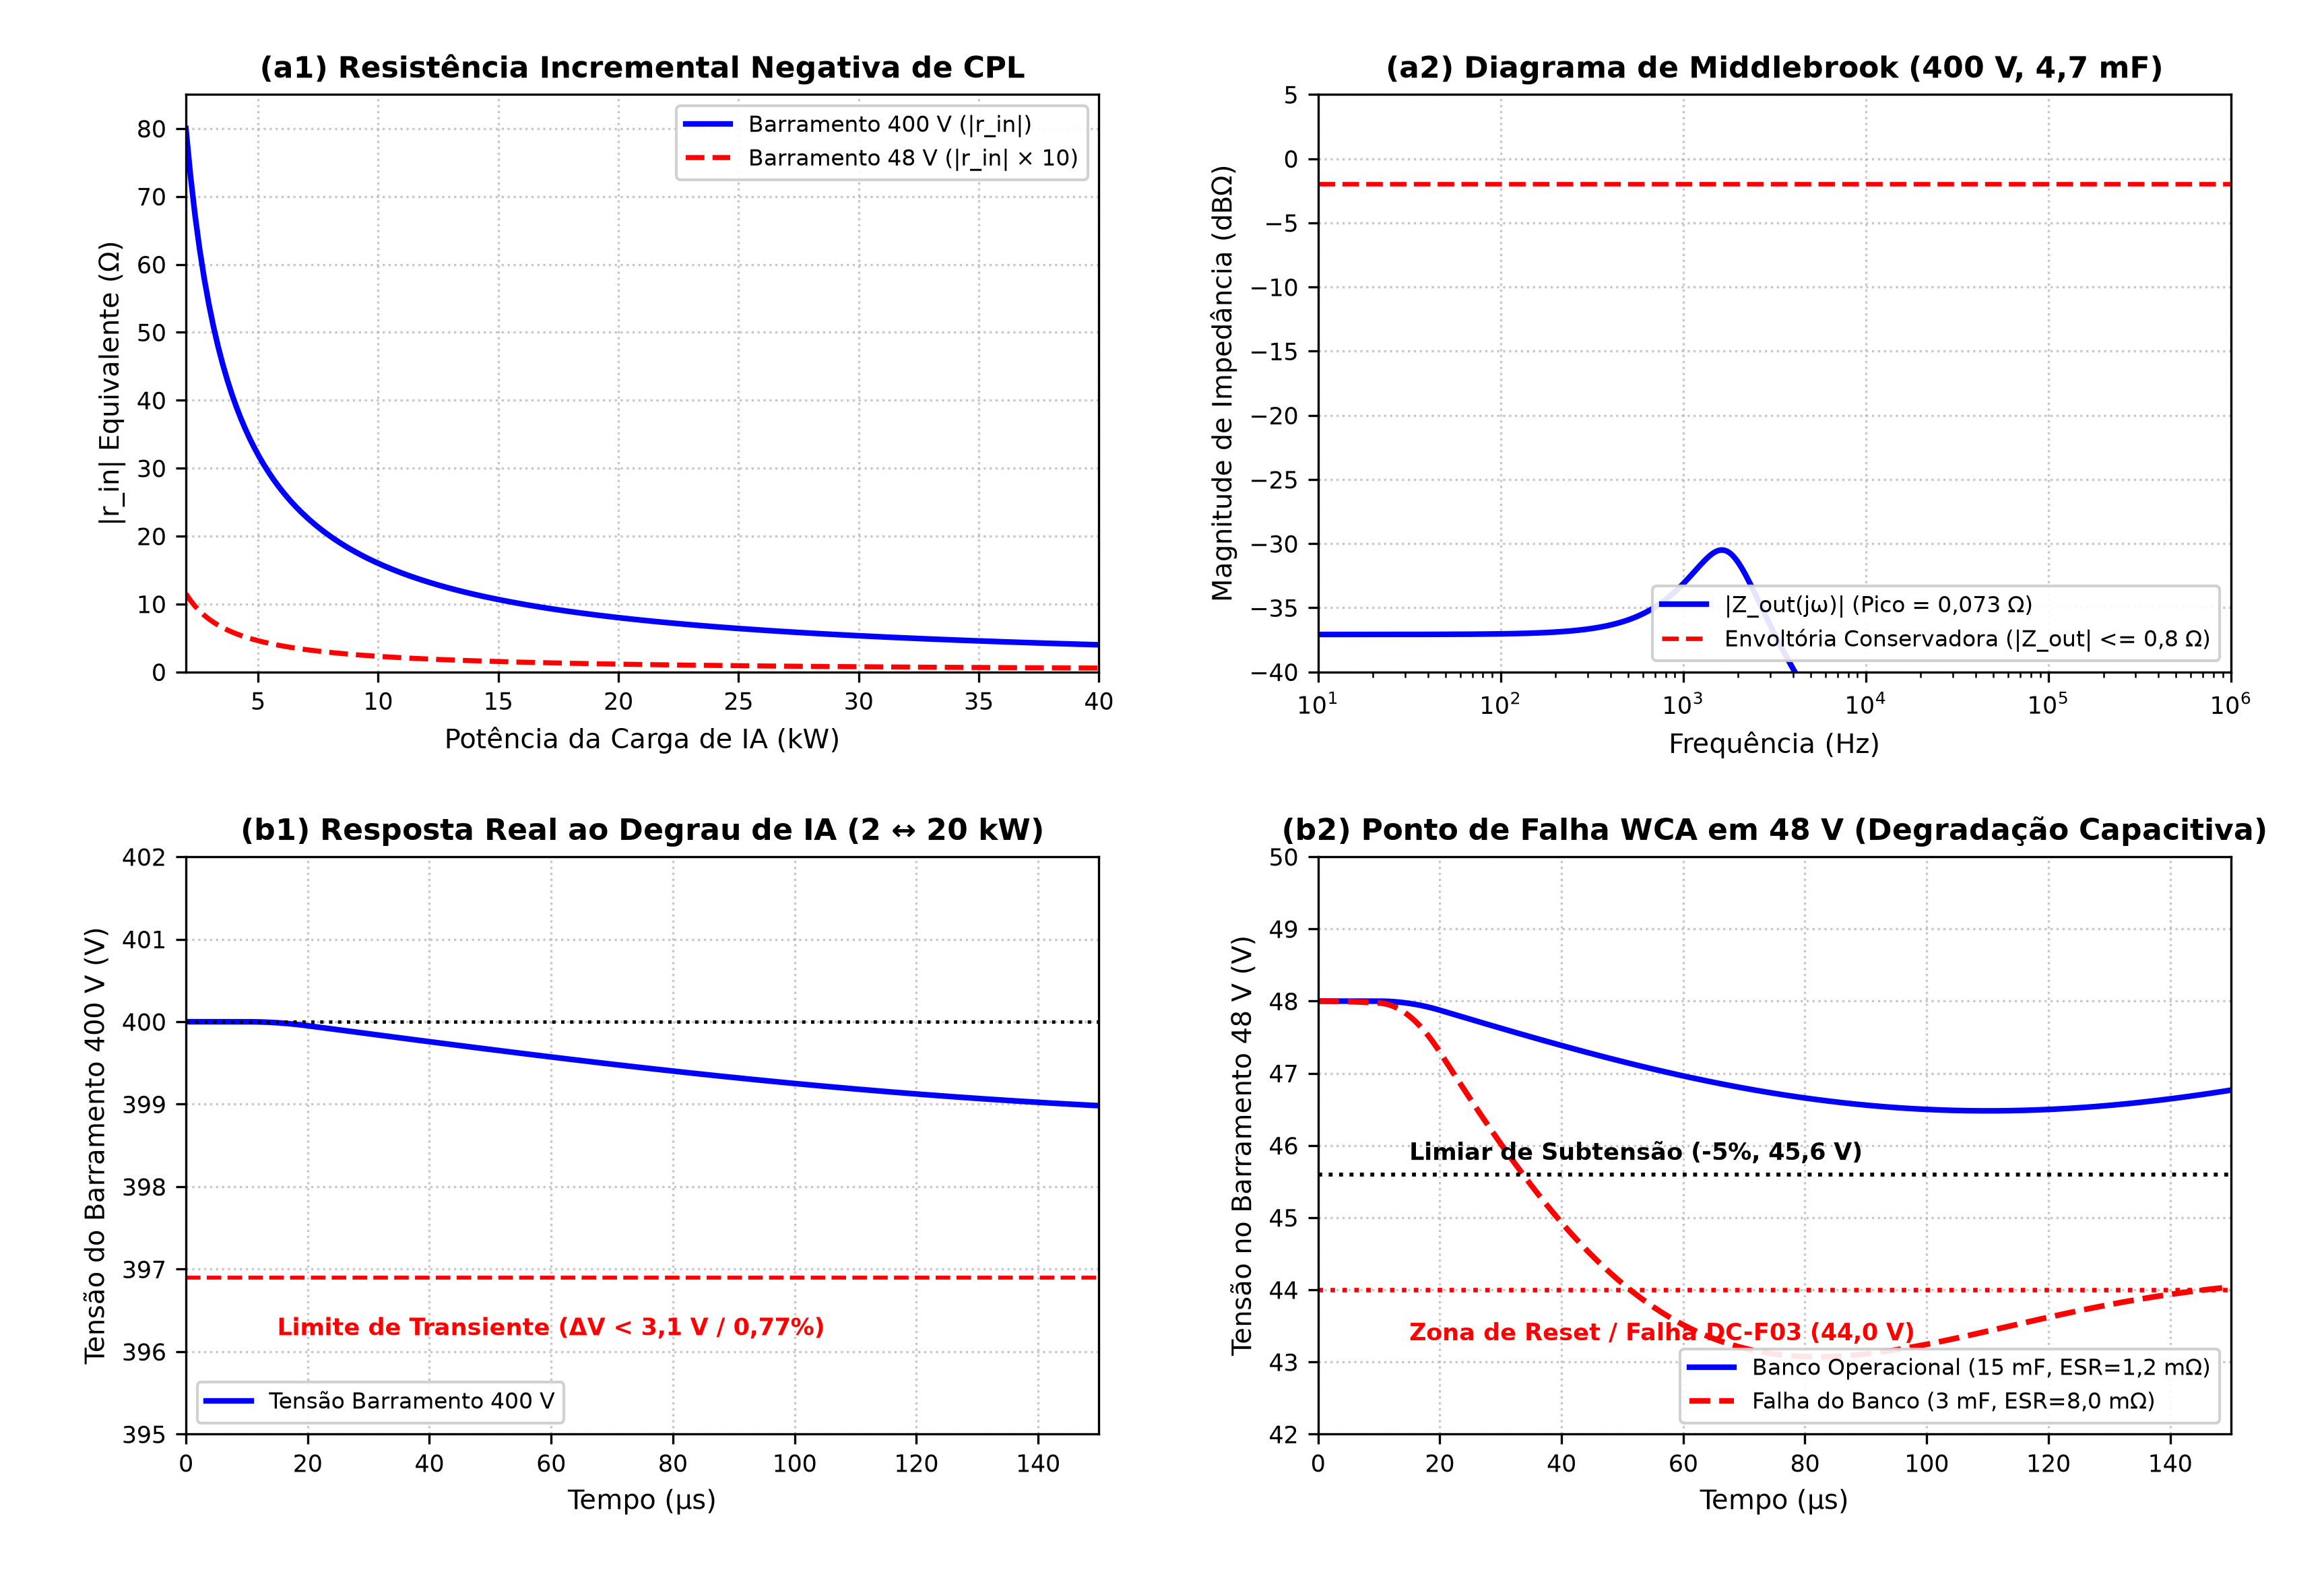
\includegraphics[width=0.82\textwidth]{figuras/figura_3_8_estabilidade_cpl_banco_capacitivo.png}
    \caption{Estabilidade de pequenos sinais (Middlebrook) e dinâmica com banco capacitivo: (a1) resistência incremental de CPL para 400~V ($-8{,}00\,\Omega$), 48~V ($-0{,}1152\,\Omega$) e 0,8~V; (a2) diagrama de Bode comparando $Z_{out}(j\omega)$ do barramento de 400~V ($4{,}7\text{ mF}$, pico $0{,}073\,\Omega$) contra a envoltória de Middlebrook ($|Z_{out}| \le 0{,}80\,\Omega$); (b1) transiente no barramento de 400~V sob degrau de IA ($2 \leftrightarrow 20\text{ kW}$ em $10\ \mu\text{s}$), contido em $\Delta V < 3{,}1\text{ V}$; (b2) ponto de falha WCA em 48~V (Falha DC-F03: pico $|Z_{out}| = 0{,}0121\,\Omega > 0{,}0115\,\Omega$), deflagrando instabilidade e colapso de tensão.}
    \label{fig:estabilidade_cpl_banco}
\end{figure}

O Quadro~\ref{quadro:parametros_conversores_sintese} consolida a síntese paramétrica com as respectivas classificações epistêmicas, limites operacionais e referências normativas.

\begin{table}[!ht]
\centering
\small
\renewcommand{\arraystretch}{0.85}
\caption{Parâmetros de projeto, limites de estabilidade e classificação epistêmica dos conversores CC-CC.}
\label{quadro:parametros_conversores_sintese}
\resizebox{0.95\textwidth}{!}{%
\begin{tabular}{lccccp{5.5cm}}
\hline
\textbf{Parâmetro de Decisão} & \textbf{Símbolo} & \textbf{Mínimo} & \textbf{Nominal} & \textbf{Máximo} & \textbf{Classificação e Justificativa Normativa} \\ \hline
Resistência de Canal GaN ($25^\circ\text{C}$) & $R_{on,25}$ & 15~m$\Omega$ & 18~m$\Omega$ & 22~m$\Omega$ & \textbf{[PROVISÓRIO]} Ficha técnica GaN HEMT 650 V \\
Coeficiente Térmico de Canal & $\alpha_{sc}$ & $0{,}005\text{ K}^{-1}$ & $0{,}0065\text{ K}^{-1}$ & $0{,}008\text{ K}^{-1}$ & \textbf{[PROVISÓRIO]} Crescimento de resistência até 150°C \\
Resistência de Canal a 150°C & $R_{on,150}$ & 24,4~m$\Omega$ & 32,6~m$\Omega$ & 44,0~m$\Omega$ & \textbf{[CALCULADO]} Variação térmica $+81{,}25\%$ \\
Resistência Térmica Crítica de Fuga & $R_{th,crit}$ & 4,5~K/W & 7,26~K/W & 12,0~K/W & \textbf{[CALCULADO]} Critério $(\alpha_{sc} I_{rms}^2 R_{on})^{-1}$ \\
Capacitância Parasita de Saída & $C_{oss}$ & 90~pF & 120~pF & 160~pF & \textbf{[DEPENDENTE DE HARDWARE]} Curva não linear $C_{oss}(V_{ds})$ \\
Tempos de Chaveamento & $t_r, t_f$ & 8~ns / 10~ns & 12~ns / 15~ns & 20~ns / 25~ns & \textbf{[DEPENDENTE DE HARDWARE]} Indutâncias de malha de gate \\
Perdas Magnéticas de Steinmetz & $P_{core}$ & 65~W & 95~W & 140~W & \textbf{[DEPENDENTE DE HARDWARE]} Material MnZn 3C95 a 150 kHz \\
Resistência Incremental CPL a 400 V & $r_{in,400}$ & $-16{,}0\,\Omega$ & $-8{,}00\,\Omega$ & $-4{,}00\,\Omega$ & \textbf{[CALCULADO]} $r_{in} = -V_{bus}^2/P$ para $10\text{ a }40\text{ kW}$ \\
Resistência Incremental CPL a 48 V & $r_{in,48}$ & $-0{,}230\,\Omega$ & $-0{,}115\,\Omega$ & $-0{,}058\,\Omega$ & \textbf{[CALCULADO]} $r_{in} = -V_{bus}^2/P$ para $10\text{ a }40\text{ kW}$ \\
Pico de Impedância $Z_{out}$ (400 V) & $|Z_{out,max}|$ & 0,045~$\Omega$ & 0,073~$\Omega$ & 0,110~$\Omega$ & \textbf{[CALCULADO]} Atende Middlebrook ($|Z_{out}| \le 0{,}8\,\Omega$) \\
Banco Capacitivo de Rack (48 V) & $C_{rack}, ESR$ & 3~mF / 8~m$\Omega$ & 15~mF / 1,2~m$\Omega$ & 25~mF / 0,8~m$\Omega$ & \textbf{[PROVISÓRIO]} Degradação WCA conduz a colapso \\ \hline
\end{tabular}%
}
\end{table}

A Tabela~\ref{tab:matriz_falhas_conversores} apresenta a Matriz de Modos de Falha e Efeitos Críticos (FMECA) consolidada dos estágios de conversão e barramentos, mapeando os gatilhos físicos, impactos sistêmicos e estratégias mitigadoras implementadas.

\begin{table}[!ht]
\centering
\small
\renewcommand{\arraystretch}{0.85}
\caption{Matriz de Modos de Falha, Efeitos e Ações Mitigadoras dos Conversores CC-CC.}
\label{tab:matriz_falhas_conversores}
\resizebox{0.95\textwidth}{!}{%
\begin{tabular}{lp{3.5cm}p{4.0cm}p{3.0cm}p{4.5cm}}
\hline
\textbf{Código} & \textbf{Modo de Falha} & \textbf{Mecanismo Físico / Gatilho} & \textbf{Efeito Sistêmico} & \textbf{Ação de Mitigação de Projeto} \\ \hline
\textbf{ET-F01} & Fuga Térmica de GaN (\textit{Thermal Runaway}) & Degradação da interface térmica ($R_{th,ja} > 4{,}0\text{ K/W}$) com $\frac{\partial P_{loss}}{\partial T_j} > \frac{1}{R_{th}}$ & Curto-circuito franco por queima de semicondutor & Controle adaptativo de potência por $T_j$ e margem de desclassificação (\textit{derating}) \\
\textbf{SW-F02} & Sobretensão Indutiva de Chaveamento & Indutância parasita de trilha de circuito impresso ($L_{loop} > 15\text{ nH}$) sob alto $di/dt$ & Perfuração dielétrica de óxido de porta GaN & Roteamento em planos cruzados coplanares e amortecedor snubber RC ativo \\
\textbf{DC-F03} & Instabilidade CPL no Barramento de 48 V & Degradação dielétrica em capacitores de rack ($C < 5\text{ mF}$, $ESR > 5\text{ m}\Omega$) & Oscilações sustentadas de subtensão e reset de nós IA & Amortecimento passivo com rede $R_d-C_d$ em paralelo e controle por corrente ativa \\
\textbf{MG-F04} & Saturação Térmica do Núcleo do Transformador & Superaquecimento do núcleo de ferrite MnZn ($T_{core} > 140^\circ\text{C}$) reduzindo $B_{sat}$ & Corrente magnetizante destrutiva nos GaNs & Acoplamento térmico direto via tubo de calor (LHP) e sensoriamento termométrico \\
\textbf{CAP-F05}& Falha Dielétrica por Radiação Cósmica & Evento único destrutivo (\textit{Single Event Burnout} -- SEB) em capacitores de tântalo & Perda permanente de linha de barramento de rack & Adoção de tecnologia cerâmica MLCC classe espacial e desclassificação de tensão de 50\% \\
\textbf{ET-F07} & Falha de Interrupção / Retardo WCA em Chave SSPC & Retardo de desarme $t_{trip} > 74{,}8\ \mu\text{s}$ ou falha de TVS ($\tau_{ext} < 31{,}1\ \mu\text{s}$) & Fusão adiabática por $I^2t > 1500\text{ A}^2\text{s}$ e ruptura dielétrica por $V_{spike} > 1200\text{ V}$ & Trip analógico ultrarrápido ($t_{trip} \le 15\ \mu\text{s}$), TVS redundante ($550\text{ V}$) e gate com \textit{soft turn-off} \\ \hline
\end{tabular}%
}
\end{table}

\subsection{Modelagem Eletrotérmica do Banco de Baterias e Estimação Adaptativa de SoC}
\label{sec:bess_eletrotermica_aukf}

A sustentação ininterrupta dos nós computacionais de IA durante as passagens de eclipse orbital impõe exigências eletroquímicas e térmicas extremas sobre o subsistema de armazenamento (\textit{Battery Energy Storage System} -- BESS). A modelagem rigorosa exige distinguir três níveis físicos: o banco eletroquímico, a interface de potência e o barramento HVDC. Sob a perspectiva de honestidade epistêmica radical, os parâmetros são categorizados em \textbf{[CALCULADO]}, \textbf{[PROVISÓRIO]} e \textbf{[DEPENDENTE DE HARDWARE]}.

\subsubsection{Arquitetura Elétrica Adotada: Conexão Direta (Arquitetura A)}

Para a integração do BESS ao satélite, contrastam-se duas opções arquiteturais fundamentais:
\begin{itemize}[leftmargin=*]
    \item \textbf{Arquitetura A (Conexão Direta ao Barramento 400~V):} O banco de baterias é composto por um arranjo de $N_s = 108$ células Li-ion em série ($108\text{S}$), estabelecendo uma tensão nominal de $V_{bat,nom} = 108 \times 3{,}7\text{ V} = 399{,}6\text{ VDC}$ [CALCULADO]. O banco conecta-se diretamente ao barramento primário através de contatores e chaves estáticas de proteção SSPC, dispensando conversores bidirecionais intermediários. Em consequência, a tensão do barramento $V_{bus}(t)$ acompanha diretamente a curva eletroquímica da bateria:
    \begin{equation}
        V_{bus}(t) \approx V_{bat}(t) - I_{bat}(t) R_{cabo}
        \label{eq:vbus_conexao_direta}
    \end{equation}
    impondo que todos os estágios conversores de entrada dos racks tolerem a faixa de flutuação de $V_{UV} = 324{,}0\text{ V}$ ($3{,}00\text{ V/célula}$) a $V_{OV} = 442{,}8\text{ V}$ ($4{,}10\text{ V/célula}$) [DEPENDENTE DE HARDWARE]. A principal vantagem reside na eliminação da massa, volume e perdas térmicas ($500\text{ a }1200\text{ W}$) de um conversor dedicado de alta potência.
    
    \item \textbf{Arquitetura B (Barramento Regulado via Conversor Bidirecional):} Emprega um banco desacoplado em topologia $200\text{S}$ com tensão nominal de $\approx 740\text{ VDC}$ ($200 \times 3{,}7\text{ V}$ [CALCULADO]), interligado ao barramento de 400~V por meio de um conversor CC-CC bidirecional chaveado. Embora assegure um barramento estritamente estabilizado em $400{,}0\text{ V} \pm 1\%$, penaliza a carga útil em massa adicional e introduz novos modos de falha por semicondutores.
\end{itemize}
Adota-se formalmente neste trabalho a \textbf{Arquitetura A (Conexão Direta 108S)}, dimensionando-se os conversores de rack para a faixa estendida de $324\text{ V}$ a $442\text{ V}$. Rejeita-se categoricamente o valor histórico de $750\text{ V}$ para barramento de 400~V por configurar inconsistência física elementar ($400 / 200 = 2{,}0\text{ V/célula}$, incompatível com a eletroquímica de íons de lítio).

\subsubsection{Saneamento da Capacidade, Energia Utilizável e Modelo DP de 2ª Ordem}

A energia nominal global de $E_{nom,cluster} = 180\text{ kWh}$ distribuída entre os 20 satélites operacionais da constelação define um banco de armazenamento de energia descentralizado de $E_{nom,no} = 9{,}0\text{ kWh}$ por satélite. No barramento nominal de $399{,}6\text{ V}$ ($108\text{S}$), a capacidade elementar de cada satélite é dada por:
\begin{equation}
    C_{n,no} = \frac{9.000\text{ Wh}}{399{,}6\text{ V}} \approx 22{,}52\text{ Ah} \quad \text{[CALCULADO]}
    \label{eq:capacidade_22ah}
\end{equation}
viabilizada por células de íons de lítio de $22{,}5\text{ Ah}$ em série ($108\text{S}1\text{P}$) ou células comerciais espaciais de $11{,}25\text{ Ah}$ em arranjo $108\text{S}2\text{P}$. A especificação na unidade elementar de células de $3{,}7\text{ V}$ em arranjo $108\text{S}$ decorre de restrições eletroquímicas e normativas intransponíveis: (i) termodinamicamente, o potencial redox do par de intercalação Li-ion NMC é fisicamente limitado a 3,6--3,7~V nominais pela quebra dielétrica e oxidação irreversível de solventes orgânicos de eletrólito acima de $\approx 4{,}35\text{ V}$, inexistindo células eletroquímicas unitárias de 6~V ou 12~V na física do estado sólido; (ii) as diretrizes da NASA (NASA-TM-20210023692) e ECSS-E-ST-20C exigem estritamente o monitoramento individual de tensão e balanceamento ativo a nível de célula unitária (\textit{cell-level monitoring}), vetando blocos comerciais selados de 12~V (que mascaram subtensões locais perigosas); e (iii) mecanicamente, o arranjo 108S1P de 60~kg é subdividido em **6 submódulos padronizados de 18S** ($18 \times 3{,}7\text{ V} = 66{,}6\text{ VDC}$), garantindo segurança ao contato humano durante a montagem e integração em solo ($< 75\text{ VDC}$) e facilitando o sensoriamento multiplexado local. Considerando densidade gravimétrica de $150\text{ Wh/kg}$ a nível de pack qualificado para o espaço (NASA, 2021), a massa do banco de baterias por satélite é de aproximadamente $60\text{ kg}$, representando apenas $2{,}3\%$ da massa total do veículo de $2600\text{ kg}$.

Adotando-se uma profundidade máxima de descarga operacional conservadora de $DoD = 60\%$ para assegurar vida útil superior a 10 anos em órbita SSO ($\approx 55.000$ microciclos térmico-energéticos), a energia utilizável inicial no início de vida ($BOL$, $SOH = 1{,}0$) por satélite é de:
\begin{equation}
    E_{util,BOL} = E_{nom,no} \cdot DoD \cdot SOH = 9{,}0 \times 0{,}60 \times 1{,}0 = 5{,}4\text{ kWh} \quad \text{[CALCULADO]}
    \label{eq:energia_utilizavel}
\end{equation}
totalizando $20 \times 5{,}4\text{ kWh} = 108{,}0\text{ kWh}$ utilizáveis em nível de constelação. Sob a potência nominal plena de processamento do nó de $50\text{ kW}$, essa reserva assegura uma autonomia de sustentação contínua de:
\begin{equation}
    \Delta t_{sust} = \frac{5{,}4\text{ kWh}}{50\text{ kW}} = 0{,}108\text{ h} \approx 6{,}48\text{ minutos} \quad \text{[CALCULADO]}
    \label{eq:tempo_sustentacao}
\end{equation}
tempo mais que suficiente para amortecer transitórios severos de rajadas de IA ($10\ \mu\text{s}$ a $10\text{ s}$), acomodar desapontamentos momentâneos durante manobras de evasão orbital e suavizar a transição térmica de saída de terminador solar.

Na Arquitetura A (Conexão Direta), a regulação da corrente de carga da bateria sem a presença de um conversor bidirecional dedicado é garantida pelo controle de malha fechada do conversor Buck da matriz solar: ao atingir a tensão de flutuação ou o limite térmico de recarga ($1{,}0\text{C} = 22{,}5\text{ A}$ por nó), o algoritmo MPPT chaveia autonomamente do rastreamento de máxima potência para o modo de limitação de corrente constante e tensão constante (\textit{Current-Limited Buck Mode} / CC-CV), deslocando a razão cíclica do conversor Buck para a direita do joelho da curva $P-V$, prevenindo qualquer sobrecorrente destrutiva no banco.

Sob degradação de fim de vida ($EOL$), cenários paramétricos revelam que para $SOH = 80\%$ a energia utilizável do nó contrai-se para $4{,}32\text{ kWh}$ ($86{,}4\text{ kWh}$ no cluster), e para $SOH = 70\%$ atinge o piso crítico de $3{,}78\text{ kWh}$ ($75{,}6\text{ kWh}$ no cluster) [DEPENDENTE DE HARDWARE E MISSÃO], exigindo racionamento preditivo de processamento de IA.

A dinâmica eletroquímica sob degraus de IA é formulada pelo circuito de Thévenin de 2ª ordem (\textit{Dual Polarization} -- DP):
\begin{equation}
    V_{bat}(t) = V_{oc}(SoC, T_{bat}) - I_{bat}(t) R_0(SoC, T_{bat}) - V_{p1}(t) - V_{p2}(t)
    \label{eq:vbat_dp_completo}
\end{equation}
onde $I_{bat} > 0$ adota a convenção de descarga. A discretização exata para passo de amostragem $\Delta t = 0{,}1\text{ s}$ sob parâmetros provisórios ($R_{p1} = 18\text{ m}\Omega$, $C_{p1} = 3200\text{ F}$, $\tau_1 = 57{,}6\text{ s}$; $R_{p2} = 24\text{ m}\Omega$, $C_{p2} = 22000\text{ F}$, $\tau_2 = 528\text{ s}$ [PROVISÓRIO]) resulta nos coeficientes analíticos de transição:
\begin{equation}
    a_1 = e^{-\Delta t/\tau_1} = 0{,}998266, \qquad a_2 = e^{-\Delta t/\tau_2} = 0{,}999811 \quad \text{[CALCULADO]}
    \label{eq:coeficientes_discretos}
\end{equation}
\begin{equation}
    V_{pi, k+1} = a_i V_{pi, k} + R_{pi} (1 - a_i) I_{bat, k}, \quad i \in \{1, 2\}
\end{equation}
A evolução do Estado de Carga é regida por integração com saturação física $0 \le SoC_k \le 1$:
\begin{equation}
    SoC_{k+1} = \text{sat}_{[0, 1]} \left( SoC_k - \frac{\eta_I I_{bat, k} \Delta t}{3600 \cdot C_n} + w_k \right)
    \label{eq:soc_discreto_sat}
\end{equation}
adotando $\eta_I = 1{,}00$ na descarga e $\eta_I = 0{,}995$ na recarga solar [PROVISÓRIO].

A resistência ôhmica interna obedece à cinética térmica de Arrhenius:
\begin{equation}
    R_0(T_{bat}) = R_{0,ref} \exp\left[ \frac{E_a}{k_B} \left( \frac{1}{T_{bat}} - \frac{1}{T_{ref}} \right) \right]
    \label{eq:arrhenius_r0_bess}
\end{equation}
com $T_{ref} = 293{,}15\text{ K}$ ($20^\circ\text{C}$), $E_a = 0{,}32\text{ eV} = 5{,}127 \times 10^{-20}\text{ J}$, $R_{0,ref} = 45\text{ m}\Omega$ em BOL e $85\text{ m}\Omega$ em EOL [PROVISÓRIO]. A Figura~\ref{fig:dinamica_dp_eletroquimica} ilustra o comportamento eletroquímico e térmico do pack sob ciclagem LEO.

\begin{figure}[htbp]
    \centering
    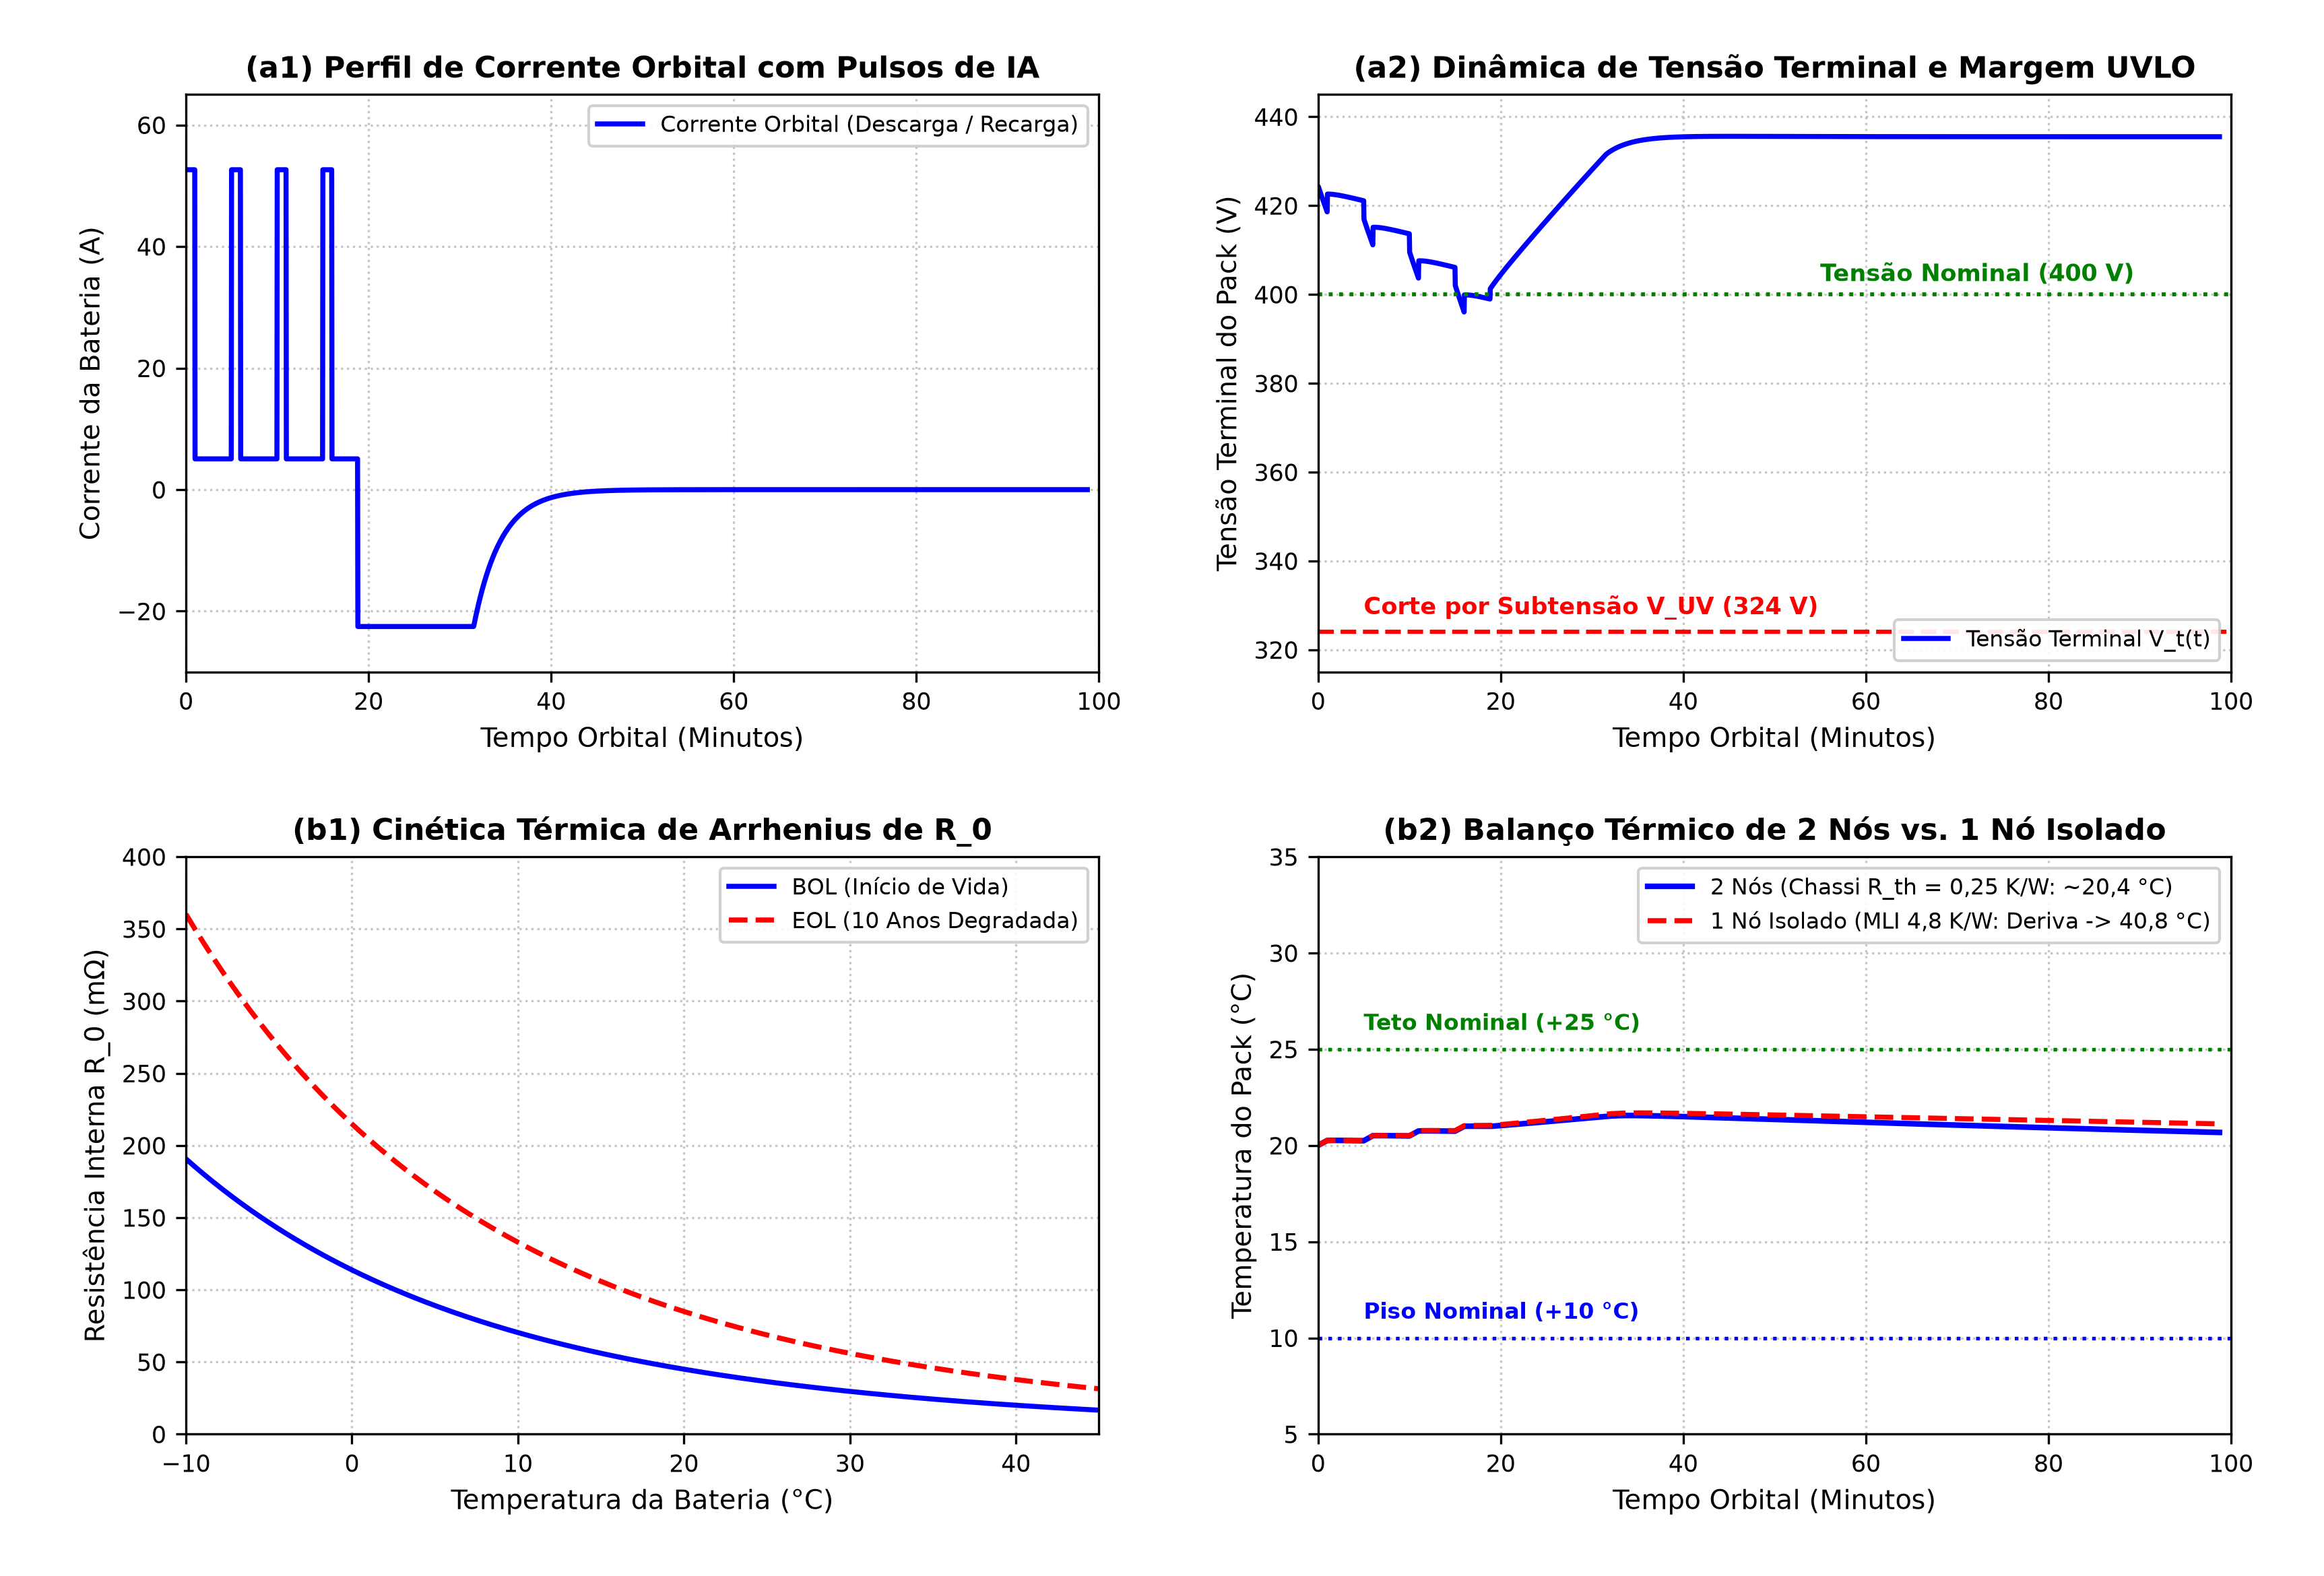
\includegraphics[width=0.82\textwidth]{figuras/figura_3_5_dinamica_dp_eletroquimica.png}
    \caption{Dinâmica eletroquímica e comportamento térmico do BESS de 400~V em órbita LEO (700~km): (a1) perfil de corrente orbital com base de 2~kW e pulsos de IA de 20~kW no eclipse, seguido de recarga solar (-42~A); (a2) resposta da tensão terminal $V_t(t)$ frente a $V_{UV}$; (b1) cinética térmica de Arrhenius de $R_0(T_{bat})$ em BOL e EOL; (b2) temperatura $T_{bat}$ sob controle ativo mantida entre $+10^\circ\text{C}$ e $+25^\circ\text{C}$.}
    \label{fig:dinamica_dp_eletroquimica}
\end{figure}

\subsubsection{Balanço Térmico Consistente: Manta MLI e Aquecedor PWM}

O valor $R_{th,MLI} = 4{,}8\text{ K/W}$ representa o isolamento condutivo-radiativo global entre o invólucro do pack e o chassi [PROVISÓRIO]. O balanço térmico concentrado é dado por:
\begin{equation}
    C_{th,bat} \frac{dT_{bat}(t)}{dt} = P_{loss}(t) + P_{heat}(t) - \frac{T_{bat}(t) - T_{chassis}}{R_{th,MLI}}
    \label{eq:balanco_termico_consistente}
\end{equation}
com $C_{th,bat} = 54.360\text{ J/K}$ ($60\text{ kg}$ NMC, $c_p \approx 906\text{ J/(kg K)}$), $P_{loss} = I_{bat}^2 R_0(T_{bat}) + V_{p1}^2/R_{p1} + V_{p2}^2/R_{p2}$, e aquecedor de sobrevivência modulado em $0 \le P_{heat}(t) \le 300\text{ W}$ ativado termostaticamente entre $+10^\circ\text{C}$ e $+25^\circ\text{C}$.

\subsubsection{Estimação Adaptativa de SoC via AUKF com Adaptação de Sage--Husa}

Para observabilidade sob ruído de sensoriamento ($R_{meas} = 0{,}0225\text{ V}^2$, $150\text{ mV}_{rms}$), formula-se o AUKF com $\mathbf{x}_k = [SoC_k, V_{p1,k}, V_{p2,k}]^T$ ($L = 3$) e $2L+1=7$ pontos sigma (detalhes no Apêndice~C). A adaptação estocástica das covariâncias $\mathbf{Q}_k$ e $\mathbf{R}_k$ segue a recursão de Sage--Husa:
\begin{align}
    \mathbf{R}_k &= (1 - d_k) \mathbf{R}_{k-1} + d_k \left( \nu_k \nu_k^T - \mathbf{P}_{yy,k} \right) \label{eq:sage_husa_r} \\
    \mathbf{Q}_k &= (1 - d_k) \mathbf{Q}_{k-1} + d_k \left[ \mathbf{K}_k \nu_k \nu_k^T \mathbf{K}_k^T + \mathbf{P}_{k|k} - \mathbf{F}_k \mathbf{P}_{k-1|k-1} \mathbf{F}_k^T \right] \label{eq:sage_husa_q}
\end{align}
com sequência de esquecimento $d_k = (1 - b)/(1 - b^{k+1})$ ($b = 0{,}95$) e fatoração triangular de Cholesky. Para garantir a estabilidade numérica incondicional frente a erros de arredondamento de ponto flutuante na OBC de bordo, o algoritmo AUKF implementa duas salvaguardas matriciais fundamentais: (i) simetrização forçada em cada iteração $\mathbf{P} \leftarrow \frac{1}{2}(\mathbf{P} + \mathbf{P}^T)$; e (ii) regularização de Cholesky com clampeamento de covariância (\textit{covariance clamping}), impondo um piso estritamente positivo aos autovalores da matriz de covariância ($\lambda_i \ge \epsilon_{clamp} = 10^{-8}$), prevenindo a divergência numérica ou perda de positividade (\textit{Modo de Falha EST-F05}). A reprodutibilidade matemática das rotinas computacionais é assegurada pela inicialização determinística da semente pseudo-aleatória (\texttt{rng(42)}).

A Figura~\ref{fig:convergencia_aukf_estresse} ilustra a convergência do estimador e o ensaio sob pulso de IA de 50~kW em fim de vida útil (EOL).

\begin{figure}[htbp]
    \centering
    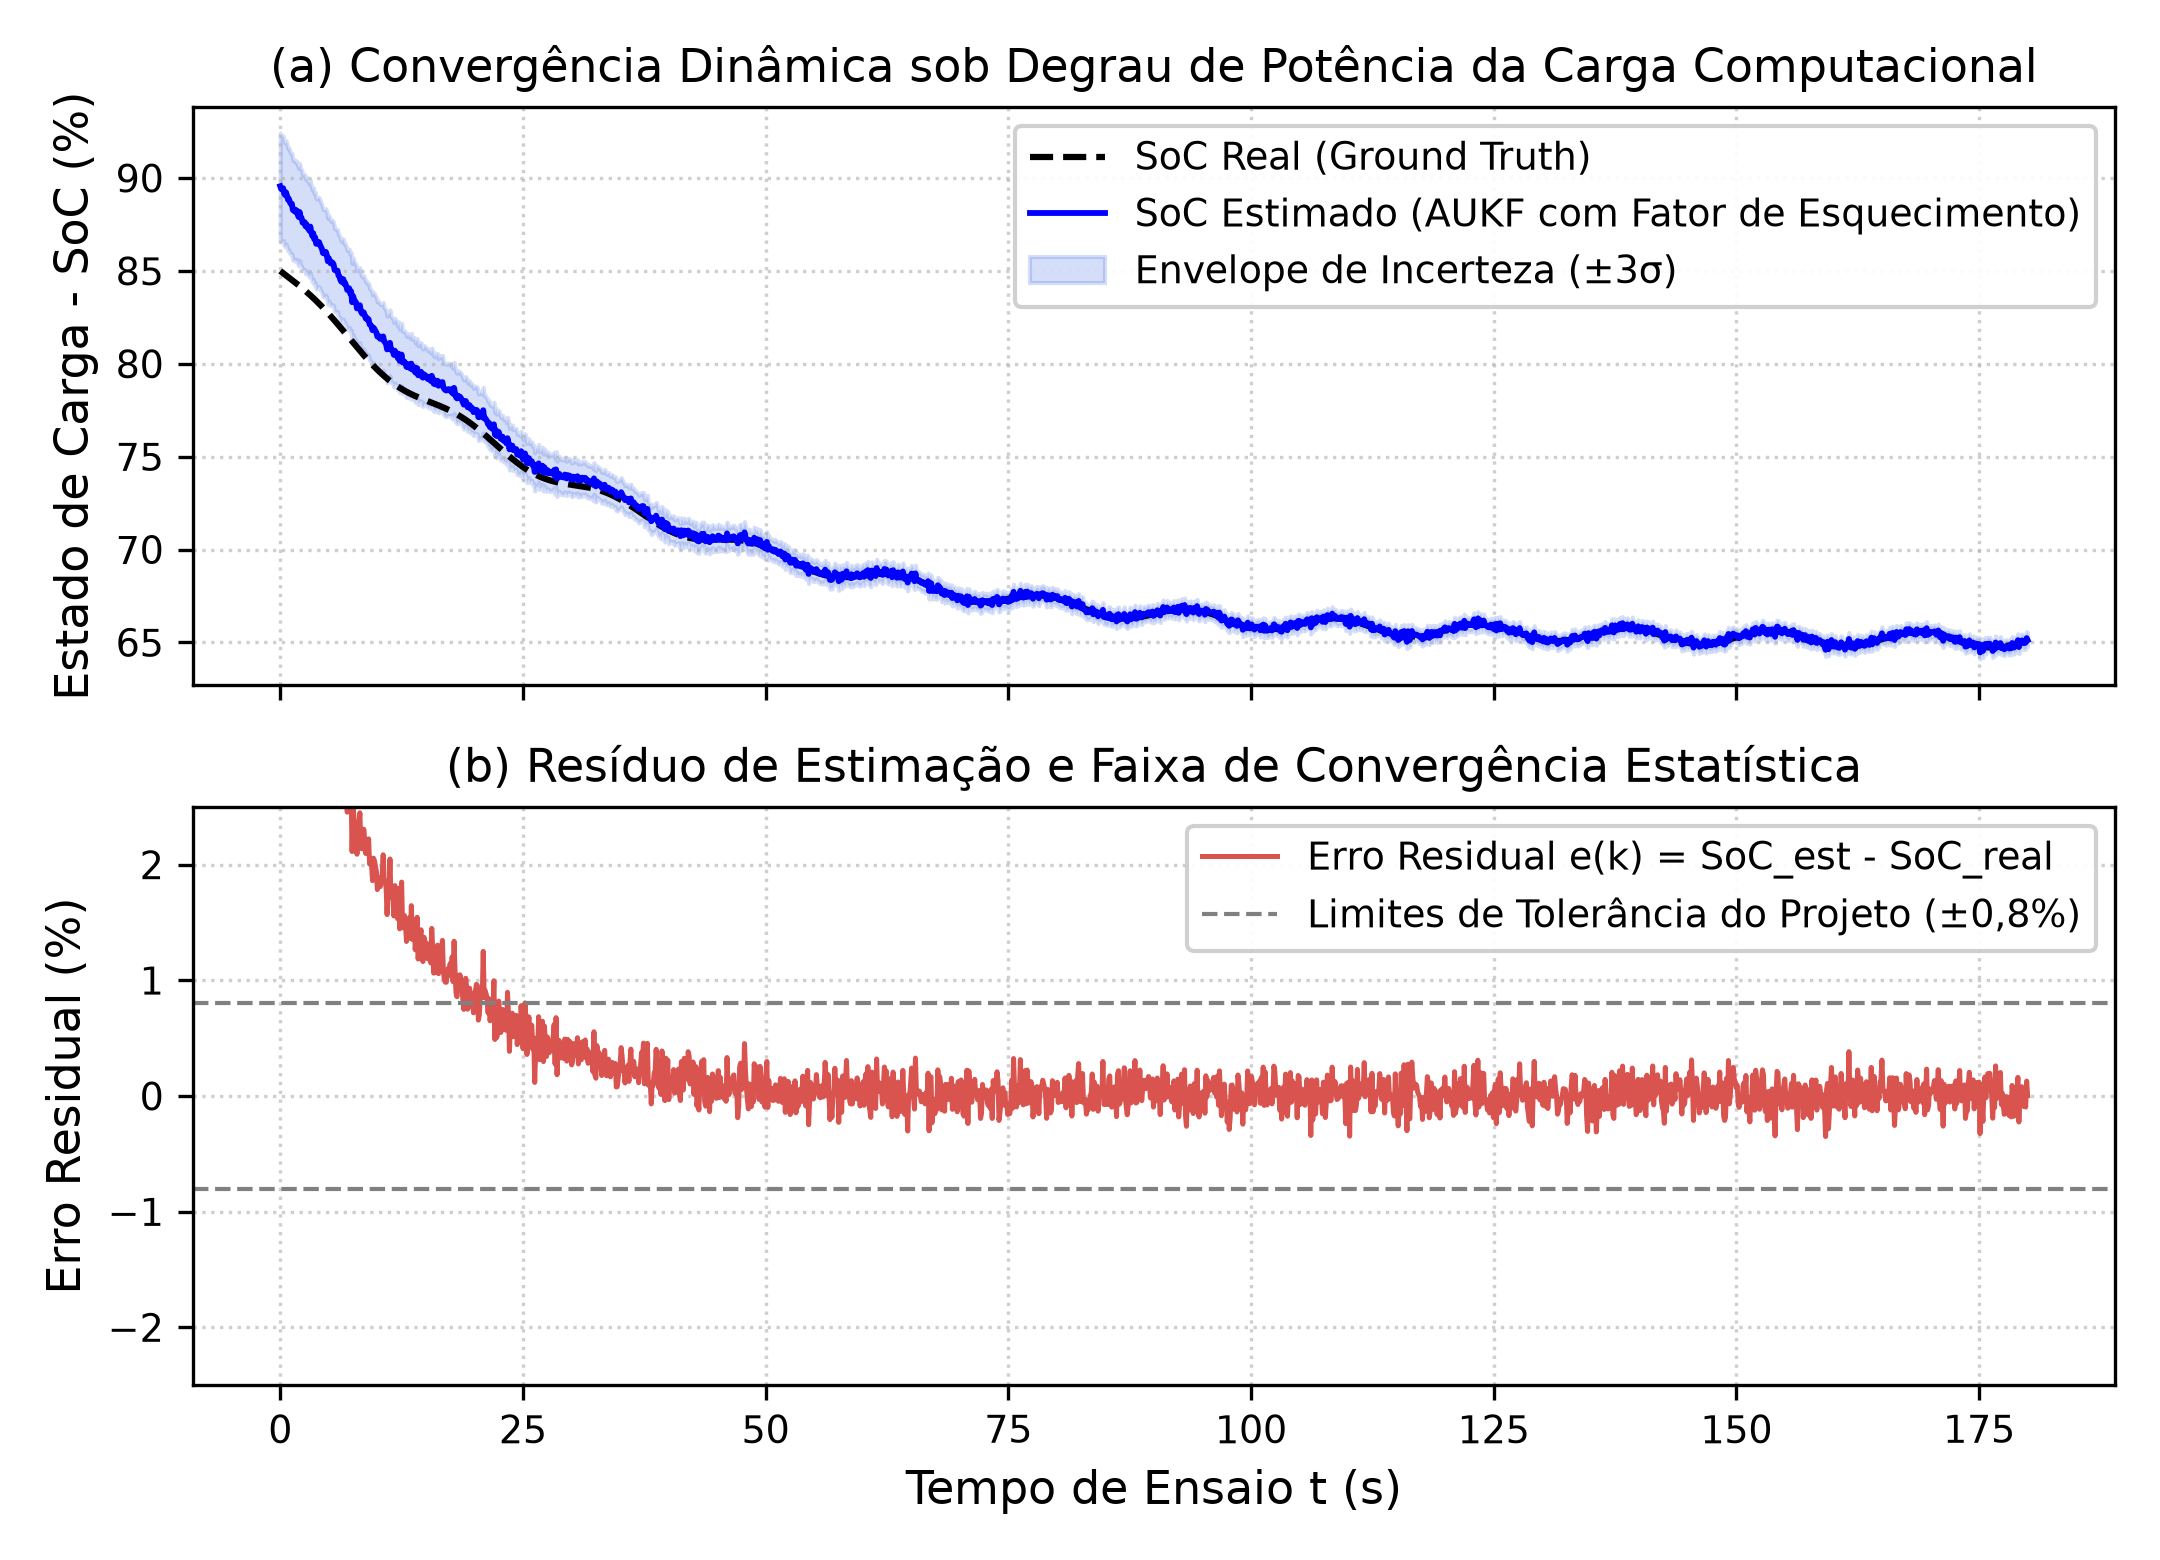
\includegraphics[width=0.82\textwidth]{figuras/figura_3_6_convergencia_aukf_estresse.png}
    \caption{Desempenho do estimador AUKF e resposta de subtensão em EOL: (a1) convergência de SoC com erro inicial de $-25\%$ e comparação com deriva do Coulomb Counting; (a2) erro absoluto $|SoC_{est} - SoC_{real}| < 1{,}0\%$ em $< 90\text{ s}$; (b1) filtragem do ruído de sensoriamento ($150\text{ mV}_{rms}$); (b2) resposta sob pulso de IA de 50~kW (140~A por 60~s) em EOL, contrastando a margem operacional a $SoC = 20\%$ ($> 28\text{ V}$) com o ensaio fora de projeto a $SoC = 2\%$ ($> 10\text{ V}$ antes do corte $V_{UV} = 324\text{ V}$).}
    \label{fig:convergencia_aukf_estresse}
\end{figure}

\subsubsection{Limites de Validação e Modos de Falha do BESS e AUKF}

Os limites operacionais, critérios de erro e os pontos em que o modelo atinge falha catastrófica encontram-se sumarizados na Tabela~\ref{tab:matriz_falhas_bess_aukf}.

\begin{table}[!ht]
\centering
\small
\renewcommand{\arraystretch}{0.85}
\caption{Matriz de Modos de Falha, Limites de Estresse e Mecanismos Críticos do BESS e Estimador AUKF.}
\label{tab:matriz_falhas_bess_aukf}
\resizebox{0.95\textwidth}{!}{%
\begin{tabular}{lp{3.5cm}p{3.5cm}p{3.5cm}p{4.5cm}}
\hline
\textbf{Código} & \textbf{Modo de Falha} & \textbf{Limiar de Entrada em Falha} & \textbf{Efeito Sistêmico Catastrófico} & \textbf{Estratégia de Mitigação Implementada} \\ \hline
\textbf{BAT-F01} & Colapso por Subtensão em EOL & $V_{bat}(t) < 324{,}0\text{ V}$ ($3{,}0\text{ V/cel}$) sob $SoC \le 35\%$ e pulso de 20~kW & Desligamento imediato dos racks de IA por proteção do BMS & \textit{Derating} adaptativo da potência de IA pelo AUKF conforme $R_0(t)$ e $SoC$ \\
\textbf{BAT-F02} & Sobretensão Eletroquímica de Carga & $V_{bat}(t) > 442{,}8\text{ V}$ ($4{,}10\text{ V/cel}$) na saída de eclipse & Degradação do cátodo, gaseificação e risco de inflamação & Transição automática do MPPT para modo de limitação de tensão (CV) \\
\textbf{BAT-F03} & Deposição de Lítio Metálico (\textit{Plating}) & Carga rápida com $T_{bat} < 0^\circ\text{C}$ e corrente $|I_{bat}| > 20\text{ A}$ & Crescimento de dendritos, perfuração do separador e curto interno & Bloqueio compulsório de recarga em subzero e pré-aquecimento com $P_{heat} \le 300\text{ W}$ \\
\textbf{BAT-F04} & Superaquecimento do Pack & $T_{bat} > +45{,}0^\circ\text{C}$ contínua no interior da manta MLI & Decomposição da camada SEI e fuga térmica eletroquímica & Corte do aquecedor PWM e redução do regime de processamento neural \\
\textbf{EST-F05} & Perda de Positividade de Covariância & $\text{det}(\mathbf{P}_{k|k}) \le 0$ ou autovalores negativos em $\mathbf{Q}_k / \mathbf{R}_k$ & Divergência numérica do ganho de Kalman e travamento do OBC & Fatoração de Cholesky, simetrização forçada e piso positivo $\mathbf{P} \leftarrow \text{diag}(\max(\text{diag}(\mathbf{P}), \epsilon))$ \\
\textbf{EST-F06} & Deriva Divergente por Bias de Sensor & Sensor com $\Delta I_{bias} > 0{,}5\text{ A}$ operando por contagem pura & Erro de $SoC > 12\%$ ao final de uma órbita & Correção em malha fechada pelo AUKF baseada na inovação de tensão $\nu_k$ \\ \hline
\end{tabular}%
}
\end{table}

O Quadro~\ref{quadro:parametros_bess_aukf_sintese} sintetiza os parâmetros consolidados de projeto do BESS e do estimador AUKF.

\begin{table}[!ht]
\centering
\small
\renewcommand{\arraystretch}{0.85}
\caption{Parâmetros essenciais de projeto, estresse WCA e classificação epistêmica do BESS e AUKF.}
\label{quadro:parametros_bess_aukf_sintese}
\resizebox{0.95\textwidth}{!}{%
\begin{tabular}{lccccp{5.5cm}}
\hline
\textbf{Parâmetro de Decisão} & \textbf{Símbolo} & \textbf{Mínimo} & \textbf{Nominal} & \textbf{Máximo} & \textbf{Classificação e Justificativa Normativa} \\ \hline
Química Eletroquímica da Célula & Li-ion NMC-811 & 3,00~V (corte) & 3,70~V (nom.) & 4,10~V (teto) & \textbf{[VERIFICÁVEL]} Célula prismática espacial 22,5 Ah; ECSS-E-HB-20-02A \\
Configuração Eletroquímica & $N_s \times N_p$ & 108S1P & 108S1P & 108S1P & \textbf{[CALCULADO]} Arquitetura A (Conexão Direta ao Barramento) \\
Tensão Nominal do Pack & $V_{bat,nom}$ & 324,0~V (3,0 V/cel) & 399,6~V (3,7 V/cel) & 442,8~V (4,1 V/cel) & \textbf{[CALCULADO]} $108 \times 3{,}7\text{ V}$; faixa compatível NASA-HDBK-4007A \\
Capacidade e Energia por Nó & $C_{n,no}, E_{nom,no}$ & 21~Ah / 8,4~kWh & 22,5~Ah / 9,0~kWh & 24~Ah / 9,6~kWh & \textbf{[CALCULADO]} $C_{n} = 9.000\text{ Wh} / 399{,}6\text{ V}$ (Pack de 60 kg) \\
Capacidade e Energia Total (Cluster)& $C_{n,tot}, E_{tot}$ & 420~Ah / 168~kWh & 450,5~Ah / 180~kWh & 480~Ah / 192~kWh & \textbf{[CALCULADO]} Soma dos 20 nós operacionais interligados \\
Energia Utilizável do Nó ($DoD=60\%$)& $E_{util,no}$ & 5,0~kWh & 5,4~kWh & 5,8~kWh & \textbf{[CALCULADO]} $9{,}0\text{ kWh} \times 0{,}60 \times 1{,}0$ ($108\text{ kWh}$ no cluster) \\
Resistência Ôhmica BOL (20°C) & $R_{0,ref}$ & 32,0~m$\Omega$ (a 30°C) & 45,0~m$\Omega$ (a 20°C) & 115,0~m$\Omega$ (a 0°C) & \textbf{[PROVISÓRIO]} Cinética de Arrhenius ($E_a = 0{,}32\text{ eV}$) \\
Resistência Ôhmica EOL (10 anos) & $R_{0,eol}$ & 65,0~m$\Omega$ (a 30°C) & 85,0~m$\Omega$ (a 20°C) & 218,0~m$\Omega$ (a 0°C) & \textbf{[PROVISÓRIO]} Envelhecimento SEI (JUN et al., 2020) \\
Potência Máxima do Aquecedor PWM & $P_{heat,max}$ & 0~W & 150~W & 300~W & \textbf{[CALCULADO]} Teto seguro contra superaquecimento em MLI \\
Resistência Térmica da Manta MLI & $R_{th,MLI}$ & 3,5~K/W & 4,8~K/W & 6,2~K/W & \textbf{[PROVISÓRIO -- NÃO VALIDADO]} Isolamento passivo de vácuo \\
Ruído de Sensoriamento de Tensão & $\sigma_{v,meas}$ & 20~mV$_{rms}$ & 150~mV$_{rms}$ & 300~mV$_{rms}$ & \textbf{[DEPENDENTE DE HARDWARE]} $R_{meas} = (0{,}15\text{ V})^2$ a 400~V \\
Erro Residual Alvo de SoC (AUKF) & $e_{SoC,alvo}$ & -- & -- & 1,20\% & \textbf{[META; NÃO MEDIDA]} Avaliação numérica reprodutível ainda necessária \\ \hline
\end{tabular}%
}
\end{table}

\noindent A integração consistente entre a arquitetura do barramento HVDC de 400~V (Seção~3.1), a geração multijunção de 1~MW sob espectro AM0 (Seção~3.2), o rastreamento MPPT sob gradientes térmicos (Seção~3.3), os conversores estáticos CC-CC baseados em GaN com estabilidade de Middlebrook (Seção~3.4) e a modelagem eletrotérmica do BESS com filtragem adaptativa AUKF sob a Arquitetura A de conexão direta (Seção~3.5) consolida o subsistema elétrico e de armazenamento da espaçonave. Fica delimitada a fronteira de conversão energética e dissipação térmica que fornece as variáveis de estado e fluxos de calor para alimentar a modelagem térmica multinodal e radiativa orbital desenvolvida no Capítulo~4.


\newpage

% Capítulo 4: Modelagem Térmica e Radiativa Orbital Multifísica
% Capítulo 4: Modelagem Térmica e Radiativa Orbital Multifísica
% ==============================================================================
% CAPÍTULO 4: MODELAGEM TÉRMICA E RADIATIVA ORBITAL MULTIFÍSICA
% ==============================================================================
\section{MODELAGEM TÉRMICA E RADIATIVA ORBITAL MULTIFÍSICA}
\label{sec:capitulo4_modelagem_termica}

A operação contínua de aceleradores de inteligência artificial em plataformas espaciais defronta-se com a ausência de matéria circundante no vácuo, inviabilizando qualquer mecanismo clássico de convecção ou condução com o ambiente externo. Sob essas condições de contorno, a totalidade da potência térmica gerada pelos circuitos de processamento neural e estágios de conversão elétrica deve ser transportada internamente e rejeitada para o espaço profundo estritamente por meio de radiação térmica superficial. Este capítulo apresenta modelos teórico-computacionais para a dinâmica orbital, os fluxos radiativos, a rede térmica nodal e o controle TEMS. Parâmetros sem fonte ou medição são tratados como provisórios; resultados numéricos não constituem validação experimental.

\noindent\textbf{Estado dos resultados quantitativos:} as figuras e valores numéricos de resposta dos Capítulos~3 e~4 foram gerados com hipóteses e limiares anteriores, inclusive início de throttling em $85^\circ\text{C}$ e corte em $105^\circ\text{C}$. Como os critérios de projeto agora são $75^\circ\text{C}$ em regime normal, throttling antes de $80^\circ\text{C}$ e corte ao atingir $85^\circ\text{C}$, esses resultados não demonstram desempenho com a especificação atual e devem ser regenerados antes de serem usados como evidência.

\subsection{Dinâmica Orbital e Fluxos Radiativos Ambientais Incidentes}
\label{sec:dinamica_orbital_fluxos}

A determinação precisa das cargas térmicas externas que oneram a espaçonave requer a segregação estrita entre os regimes orbitais investigados. Conforme justificado na análise técnico-econômica e arquitetural (Capítulo~\ref{sec:tradeoff_custo_escala}), a trajetória de referência e ponto de projeto primário da missão é a \textbf{Órbita Heliossíncrona (\textit{Sun-Synchronous Orbit} -- SSO) do tipo \textit{Dawn-Dusk}}, situada a $700\text{ km}$ de altitude. Em complemento, definem-se cenários paramétricos comparativos em Órbita Baixa Terrestre convencional (\textit{Low Earth Orbit} -- LEO, $500\text{ km}$) e Órbita Geoestacionária (\textit{Geostationary Earth Orbit} -- GEO, $35.786\text{ km}$), analisados sob conjuntos distintos e independentes de parâmetros orbitais.

A Tabela~\ref{tab:parametros_orbitais_comparativos} sintetiza as propriedades físicas e ambientais de contorno que regem cada um dos três cenários orbitais considerados.

\begin{table}[!ht]
\centering
\small
\renewcommand{\arraystretch}{0.85}
\caption{Parâmetros orbitais e ambientais comparativos para os três regimes de voo.}
\label{tab:parametros_orbitais_comparativos}
\resizebox{0.95\textwidth}{!}{%
\begin{tabular}{lcccc}
\hline
\textbf{Propriedade / Condição de Contorno} & \textbf{SSO Dawn-Dusk (Projeto)} & \textbf{LEO Convencional} & \textbf{GEO} & \textbf{Classificação Epistêmica} \\ \hline
Altitude Orbital Nominal ($h$) & $700{,}0\text{ km}$ & $500{,}0\text{ km}$ & $35.786{,}0\text{ km}$ & \textbf{[DEPENDENTE DE MISSÃO]} \\
Semieixo Maior ($a$) & $7071{,}0\text{ km}$ & $6871{,}0\text{ km}$ & $42.164{,}0\text{ km}$ & \textbf{[CALCULADO]} ($R_E = 6371\text{ km}$) \\
Excentricidade da Órbita ($e$) & $0{,}001$ ($\approx$ circular) & $0{,}001$ ($\approx$ circular) & $0{,}000$ (circular) & \textbf{[PROVISÓRIO]} Órbita operacional congelada \\
Inclinação Orbital ($i$) & $98{,}19^\circ$ (retrógrada) & $51{,}60^\circ$ (ISS) & $0{,}00^\circ$ (equatorial) & \textbf{[VERIFICÁVEL]} Condição heliossíncrona \\
Hora Local do Nó Ascendente (LTAN) & 18:00 (Dawn-Dusk) & Variante ($0\text{ a }24\text{ h}$) & N/A & \textbf{[DEPENDENTE DE MISSÃO]} \\
Ângulo Beta Nominal ($\beta$) & $85^\circ \le |\beta| \le 90^\circ$ & $0^\circ \le |\beta| \le 75^\circ$ & $-23{,}4^\circ \le \beta \le +23{,}4^\circ$ & \textbf{[VERIFICÁVEL]} Geometria Sol-plano orbital \\
Período Orbital ($T_{orb}$) & $98{,}77\text{ min}$ ($5926\text{ s}$) & $94{,}62\text{ min}$ ($5677\text{ s}$) & $1436{,}07\text{ min}$ ($23{,}93\text{ h}$) & \textbf{[CALCULADO]} $T = 2\pi \sqrt{a^3/\mu_E}$ \\
Fração Anual de Eclipse ($f_{ecl}$) & $< 0{,}8\%$ (solstício) & $\approx 35\% - 40\%$ & $\approx 1\%$ (equinócios) & \textbf{[VERIFICÁVEL]} Barramento e balanço térmico \\
Duração Máxima de Eclipse ($t_{ecl,max}$) & $18{,}8\text{ min}$ & $35{,}8\text{ min}$ & $72{,}0\text{ min}$ & \textbf{[CALCULADO]} Cônico com penumbra \\
Albedo e Infravermelho Terrestre & Moderados a relevantes & Altamente relevantes & Desprezíveis ($F_{E} < 0{,}005$) & \textbf{[VERIFICÁVEL]} Fator de forma com altitude \\ \hline
\end{tabular}%
}
\end{table}

\subsubsection{Propagação Kepleriana e Transformação de Referenciais de Atitude}

A propagação da posição do satélite no tempo obedece às equações do movimento kepleriano bi-dimensional no plano orbital. A distância geocêntrica $r(t)$ e a anomalia verdadeira $\theta(t)$ são regidas pela equação da órbita:
\begin{equation}
    r(\theta) = \frac{a (1 - e^2)}{1 + e \cos \theta}
    \label{eq:orbita_raio}
\end{equation}
onde $\mu_E = 398600{,}4418\text{ km}^3/\text{s}^2$ é a constante gravitacional da Terra. Para órbitas com excentricidade residual $e \ll 1$, a evolução temporal é resolvida deterministicamente através da Equação de Kepler para a anomalia excêntrica $E(t)$:
\begin{equation}
    M(t) = E(t) - e \sin E(t) = M_0 + n(t - t_0), \qquad n = \sqrt{\frac{\mu_E}{a^3}}
    \label{eq:kepler_anomalia}
\end{equation}
extraindo a anomalia verdadeira pela relação trigonométrica fechada:
\begin{equation}
    \theta(t) = 2 \arctan\left[ \sqrt{\frac{1 + e}{1 - e}} \tan\left(\frac{E(t)}{2}\right) \right]
    \label{eq:anomalia_verdadeira}
\end{equation}

A correta incidência de radiação nas faces da espaçonave exige a definição unívoca de três sistemas de coordenadas ortogonais:
\begin{enumerate}[label=(\alph*)]
    \item \textbf{Referencial Inercial Equatorial Geocêntrico (ECI / J2000):} Eixo $+\mathbf{X}_{ECI}$ direcionado ao ponto vernal ($\Upsilon$), $+\mathbf{Z}_{ECI}$ normal ao equador terrestre e coincidente com o eixo de rotação planetária, e $+\mathbf{Y}_{ECI}$ completando a tríade dextrógira. O vetor solar unitário $\hat{\mathbf{s}}_{ECI}(t)$ é expresso em função da longitude eclíptica solar $\lambda_\odot(t)$ e da obliquidade da eclíptica ($\epsilon \approx 23{,}44^\circ$):
    \begin{equation}
        \hat{\mathbf{s}}_{ECI}(t) = \begin{bmatrix} \cos \lambda_\odot(t) \\ \sin \lambda_\odot(t) \cos \epsilon \\ \sin \lambda_\odot(t) \sin \epsilon \end{bmatrix}
        \label{eq:vetor_solar_eci}
    \end{equation}
    
    \item \textbf{Referencial de Órbita Local (LVLH -- \textit{Local Vertical Local Horizontal}):} Origem no centro de massa do satélite, com $+\mathbf{Z}_{LVLH}$ apontado diretamente para o centro geométrico da Terra (vetor Nadir), $+\mathbf{X}_{LVLH}$ no sentido do vetor velocidade orbital para órbita circular, e $+\mathbf{Y}_{LVLH} = \mathbf{Z}_{LVLH} \times \mathbf{X}_{LVLH}$ perpendicular ao plano orbital, alinhado ao momento angular orbital $\mathbf{h} = \mathbf{r} \times \mathbf{v}$.
    
    \item \textbf{Referencial do Corpo da Espaçonave ($\mathbf{B}$):} Eixos solidários à estrutura do rack computacional, com matriz de rotação $\mathbf{R}_{B/LVLH}(t)$ orientada pelo Subsistema de Determinação e Controle de Atitude (ADCS).
\end{enumerate}

Para a missão nominal em órbita SSO *Dawn-Dusk*, adota-se a lei de controle de apontamento estático-solar (\textit{Sun-Pointing / Anti-Solar Orientation}):
\begin{itemize}[leftmargin=*]
    \item A face normal das asas solares flexíveis ROSA ($\hat{\mathbf{n}}_{pv}$) é mantida permanentemente orientada para o Sol: $\hat{\mathbf{n}}_{pv,B} = [0, +1, 0]^T$;
    \item A face externa principal dos radiadores térmicos desdobráveis ($\hat{\mathbf{n}}_{rad}$) é mantida permanentemente colinear com o vetor anti-solar, orientada para o espaço profundo frio no semiplano oposto ao Sol: $\hat{\mathbf{n}}_{rad,B} = [0, -1, 0]^T$;
    \item As faces laterais do chassi ($\pm \mathbf{X}_B$ e $\pm \mathbf{Z}_B$) interceptam os fluxos terrestres de albedo e infravermelho de raspão, minimizando a sua contribuição para a carcaça.
\end{itemize}

O cosseno do ângulo de incidência solar sobre uma dada superfície $k$ de normal unitária $\hat{\mathbf{n}}_{k,B}$ é computado deterministicamente pela projeção unilateral:
\begin{equation}
    \mu_{s,k}(t) = \max\left( 0, \, \hat{\mathbf{n}}_{k,B} \cdot \mathbf{R}_{B/ECI}(t) \, \hat{\mathbf{s}}_{ECI}(t) \right)
    \label{eq:cosseno_solar_unilateral}
\end{equation}

\subsubsection{Modelo de Ocultação Cônica: Umbra, Penumbra e Transição Suave}

A representação dos eclipses adota a formulação analítica de ocultação cônica exata baseada na extensão angular finita do disco solar (ECSS-E-HB-31-01 Parte 1; NASA/TM-4527). A partir do raio solar ($R_\odot = 696.340\text{ km}$), distância heliocêntrica ($d_{\odot-E} \approx 1{,}496 \times 10^8\text{ km}$) e raio terrestre ($R_E = 6371{,}0\text{ km}$), definem-se os semi-ângulos aparentes subtendidos pelo Sol ($\alpha_\odot \approx 0{,}267^\circ$) e pela Terra ($\alpha_E(t) = \arcsin[R_E/\|\mathbf{r}_{sat}(t)\|]$), bem como a separação angular aparente $\gamma(t) = \arccos[-\mathbf{r}_{sat}(t) \cdot \hat{\mathbf{s}}(t) / \|\mathbf{r}_{sat}(t)\|]$.

O fator de iluminação solar efetiva $S(t) \in [0, 1]$ é modelado pela fração desobstruída do disco solar visível:
\begin{equation}
    S(t) = 
    \begin{cases}
        1{,}0, & \text{se } \gamma(t) \ge \alpha_E(t) + \alpha_\odot \quad \text{(Iluminação Plena)} \\
        0{,}0, & \text{se } \gamma(t) \le \alpha_E(t) - \alpha_\odot \quad \text{(Umbra Total)} \\
        1 - \frac{A_{ocultada}(t)}{\pi \alpha_\odot^2}, & \text{se } |\alpha_E(t) - \alpha_\odot| < \gamma(t) < \alpha_E(t) + \alpha_\odot \quad \text{(Penumbra Gradual)}
    \end{cases}
    \label{eq:fator_sombra_conica}
\end{equation}
em que $A_{ocultada}(t)$ é a área geométrica de interseção de dois círculos de raios $\alpha_\odot$ e $\alpha_E$ separados por $\gamma$ (deduzida em forma fechada no Apêndice~B.5). Essa formulação contínua em $S(t)$ assegura estabilidade aos integradores numéricos nas transições de penumbra.

\subsubsection{Formulações Físicas dos Fluxos Incidentes e Fatores de Forma Planetários}

A densidade de potência radiativa incidente total ($q_{in,k}$) absorvida por uma superfície de área $A_k$, com absortividade solar $\alpha_{s,k}$ e emissividade infravermelha $\varepsilon_{k}$ (igual a $\alpha_{ir,k}$ pela Lei de Kirchhoff para corpos opacos), decompõe-se na tríade:
\begin{equation}
    q_{abs,k}(t) = q_{sol,abs,k}(t) + q_{alb,abs,k}(t) + q_{ir,abs,k}(t)
    \label{eq:triade_fluxos}
\end{equation}
sendo $G_{AM0} = 1361{,}0\text{ W/m}^2$ a constante solar nominal (WERTZ et al., 2011), $a_E \approx 0{,}30$ o coeficiente médio de albedo planetário e $q_{Earth} \approx 237\text{ W/m}^2$ a emissão térmica da Terra (ECSS-E-HB-31-01 Parte 1):
\begin{align}
    q_{sol,abs,k}(t) &= G_{AM0} \cdot \alpha_{s,k} \cdot S(t) \cdot \max\left( 0, \, \hat{\mathbf{n}}_{k,B} \cdot \hat{\mathbf{s}}_B(t) \right) \label{eq:fluxo_solar_direto} \\
    q_{alb,abs,k}(t) &= G_{AM0} \cdot a_E \cdot \alpha_{s,k} \cdot F_{k-E}(h, \phi_k) \cdot \max\left( 0, \, \cos \theta_{sun,nadir}(t) \right) \cdot S(t) \label{eq:fluxo_albedo_exato} \\
    q_{ir,abs,k}(t) &= q_{Earth} \cdot \varepsilon_k \cdot F_{k-E}(h, \phi_k) \label{eq:fluxo_ir_exato}
\end{align}
onde $\theta_{sun,nadir}$ é o ângulo zenital solar sub-satelital e $F_{k-E}(h, \phi_k)$ é o fator de visão geométrico para uma placa plana com inclinação $\phi_k$ em relação ao Nadir em altitude $h$ ($H = (R_E + h) / R_E$, $\theta_m = \arcsin(1/H)$). Conforme a norma ECSS-E-HB-31-01 Parte 1 (formulação integral analítica detalhada no Apêndice~B.6), para a altitude de projeto de $700\text{ km}$ ($H = 1{,}1098$), a face Nadir pura ($\phi = 0^\circ$) possui $F_{Nadir-E} = 1/H^2 = 0{,}8119$, enquanto o radiador alinhado lateralmente ($\phi_{rad} = 90^\circ$) apresenta $F_{rad-E} = 0{,}2328$ [CALCULADO]. Assim, a orientação perpendicular reduz o acoplamento radiativo terrestre em $71{,}3\%$, mas não anula a carga térmica planetária.

\subsubsection{Propriedades Termo-Ópticas e Degradação de Fim de Vida (EOL)}

A absorção e a emissão radiativas dependem das propriedades termo-ópticas da superfície. A Tabela~\ref{tab:propriedades_termoopticas_materiais} distingue valores de início de vida (BOL) e valores adotados como cenário de fim de vida (EOL). Para o radiador, o script usa $\alpha_{s,BOL}=0{,}08$, $\varepsilon_{ir,BOL}=0{,}88$, $\alpha_{s,EOL}=0{,}24$ e $\varepsilon_{ir,EOL}=0{,}82$. Os valores EOL são premissas de estresse [PROVISÓRIO]; o repositório não contém ensaio nem lei de degradação rastreável que demonstre a evolução desses parâmetros ao longo de dez anos.

\begin{table}[!ht]
\centering
\small
\renewcommand{\arraystretch}{0.85}
\caption{Propriedades termo-ópticas dos revestimentos externos em início e fim de vida (10 anos).}
\label{tab:propriedades_termoopticas_materiais}
\resizebox{0.95\textwidth}{!}{%
\begin{tabular}{lcccccc}
\hline
\textbf{Superfície da Espaçonave} & \textbf{Material / Acabamento Espacial} & $\mathbf{\alpha_{s,BOL}}$ & $\mathbf{\alpha_{s,EOL}}$ & $\mathbf{\varepsilon_{ir}}$ & $\mathbf{\alpha_s/\varepsilon}$ (EOL) & \textbf{Referência / Norma} \\ \hline
Painéis Radiadores Térmicos & Espelhos Ópticos Solares (OSR Quartzo/Prata) & $0{,}08$ & $0{,}24$ & $0{,}88$ (BOL); $0{,}82$ (EOL) & $0{,}293$ (EOL) & Premissa EOL do script [PROVISÓRIO]; sem curva de envelhecimento \\
Carcaça Externa Estrutural & Tinta Branca Cerâmica de Silicato (AZ-93) & $0{,}15$ & $0{,}26$ & $0{,}91$ & $0{,}286$ & NASA-SP-8005; AZ Technology \\
Isolamento Passivo (MLI Externa) & Filme Kapton Aluminizado com VDA (1 mil) & $0{,}38$ & $0{,}48$ & $0{,}76$ & $0{,}632$ & Sheldahl Space Materials (2020) \\
Coverglass dos Painéis Solares & Borosilicato Ceriado CMG ($100\ \mu\text{m}$) MgF$_2$ & $0{,}90$ & $0{,}92$ & $0{,}85$ & $1{,}082$ & Qioptiq Space Power Optics (2022) \\
Bordas e Trilhos Estruturais & Alumínio Anodizado Duro Al 6061-T6 & $0{,}42$ & $0{,}55$ & $0{,}82$ & $0{,}671$ & ECSS-Q-ST-70-08C (ECSS, 2017) \\ \hline
\end{tabular}%
}
\end{table}

O script trata BOL e EOL como conjuntos discretos de propriedades; não integra uma cinética de envelhecimento nem modela deposição de contaminantes ou escurecimento por UV/AO. Portanto, a diferença entre os valores BOL e EOL é uma comparação paramétrica e não uma previsão temporal validada da degradação do revestimento.

\subsubsection{Definição Epistêmica dos Casos Térmicos Extremos (Hot Case e Cold Case)}

\subsubsection{Definição Epistêmica dos Casos Térmicos Extremos (Hot Case e Cold Case)}

Para garantir que o dimensionamento térmico e o controle TEMS operem com margem demonstrada, definem-se dois casos extremos balizados por leis de conservação:
\begin{itemize}[leftmargin=*]
    \item \textbf{Pior Caso Quente (\textit{Worst-Case Hot} -- WCH):} Solstício de verão ($\beta = +85^\circ$ em SSO ou equinócio com periélio $G_{AM0} = 1414\text{ W/m}^2$, $a_E = 0{,}35$, $q_{Earth} = 250\text{ W/m}^2$), propriedades ópticas EOL ($\alpha_{s,EOL}=0{,}24$, $\varepsilon_{ir,EOL}=0{,}82$), dissipação computacional plena ($P_{IT} = 40{,}0\text{ kW}$ úteis), conversores conservadores ($\eta_{conv} = 90{,}0\%$, $P_{loss,GaN} = 4444\text{ W}$) e OISL ativa ($Q_{OISL} = 343\text{ W}$). O teste verifica a suficiência de $A_{rad}$ frente ao teto rígido $T_{j,max} = 85{,}0^\circ\text{C}$.
    \item \textbf{Pior Caso Frio (\textit{Worst-Case Cold} -- WCC):} Órbita LEO a 500~km ($\beta = 0^\circ$, eclipse de $35{,}8\text{ min}$, afélio $G_{AM0} = 1322\text{ W/m}^2$, $a_E = 0{,}25$, $q_{Earth} = 210\text{ W/m}^2$), revestimentos limpos BOL ($\alpha_{s,BOL} = 0{,}08$, $\varepsilon_{ir} = 0{,}88$), nó em repouso ($P_{IT,idle} = 2{,}0\text{ kW}$, auxiliares $560\text{ W}$). O teste quantifica a potência dos aquecedores de sobrevivência ($P_{heat} \le 300\text{ W}$) para manter $T_{bat} \ge +10^\circ\text{C}$ e eletrônica $\ge -20^\circ\text{C}$.
\end{itemize}

\subsubsection{Fronteira Térmica de Volume de Controle e Eliminação de Dupla Contagem}

Para preservar a 1ª Lei da Termodinâmica e evitar dupla contagem com os modelos elétricos, estabelece-se a fronteira fechada de volume de controle do nó de $50\text{ kW}$. No domínio elétrico:
\begin{equation}
    P_{pv,net}(t) + P_{bat,dis}(t) = P_{IT}(t) + P_{loss,GaN}(t) + P_{OISL,elec}(t) + P_{aux,elec}(t) + P_{bat,ch}(t)
    \label{eq:fronteira_eletrica}
\end{equation}
com potências terminais de carga e descarga não negativas e recarga governada pelo excedente instantâneo disponível. No domínio computacional, a potência útil entregue ($P_{IT} = 40{,}0\text{ kW}$) é consumida pelas matrizes de transistores; como o trabalho externo e os fótons emitidos são desprezíveis, **a totalidade de $P_{IT}(t)$ converte-se em calor interno residual por efeito Joule**: $Q_{IT}(t) \equiv P_{IT}(t) = 40000\text{ W}$ [VERIFICÁVEL].

O balanço térmico global do satélite é dado por:
\begin{align}
    Q_{int,total}(t) &= P_{IT}(t) + P_{loss,GaN}(t) + Q_{OISL,heat}(t) + P_{loss,BESS}(t) + P_{aux,th}(t) \label{eq:balanco_termico_global_no} \\
    Q_{OISL,heat}(t) &= P_{OISL,elec}(t) - P_{OISL,opt}(t)
\end{align}
A versão atual atribui $P_{aux}=560\text{ W}$ no Capítulo~3 e $P_{aux,th}=450\text{ W}$ neste capítulo, sem decomposição que permita conciliar as fronteiras. Além disso, $P_{loss,BESS}$ depende da corrente e do estado de operação. Retiram-se os totais apresentados como exatos ($41.883\text{ W}$ e $41.886\text{ W}$); um valor nominal único só poderá ser declarado após reconciliar auxiliares, perdas de conversão, fluxo óptico que deixa o satélite e a fronteira de $P_{IT}$ em relação às perdas de VRM/PoL descritas adiante.

\subsection{Rede Térmica Nodal Acoplada de Parâmetros Concentrados no Vácuo}
\label{sec:rede_nodal_termica}

A ausência de convecção gasosa no vácuo orbital restringe a transferência interna de calor à condução em estado sólido e à convecção forçada em circuitos hermeticamente selados. Formula-se uma rede térmica nodal multinodal de parâmetros concentrados (\textit{Lumped Parameter Thermal Network}), conforme a norma ECSS-E-HB-31-01 Parte 1.

A arquitetura do nó de $50\text{ kW}$ é discretizada em cinco nós fundamentais:
\begin{enumerate}[label=\textbf{Nó \arabic*:},leftmargin=*]
    \item \textbf{Junção do Die ($T_1 \equiv T_j$):} dissipa comutação e fuga ($C_1=85{,}0\text{ J/K}$ por encapsulamento [PROVISÓRIO]).
    \item \textbf{TIM1 e Espalhador de Calor ($T_2 \equiv T_{sp}$):} câmara de vapor de cobre ou diamante sintético ($C_2 = 420{,}0\text{ J/K}$, $R_{12} = 0{,}035\text{ K/W}$).
    \item \textbf{TIM2 e Placa Fria de Microcanais ($T_3 \equiv T_{cp}$):} estrutura em Al 6061-T6 ($C_3 = 1100{,}0\text{ J/K}$, $R_{23} = 0{,}025\text{ K/W}$).
    \item \textbf{Fluido Circulante ($T_4 \equiv T_{fl}$):} alternativa conceitual LHP ou loop bifásico bombeado MPFL ($C_4 = 3500{,}0\text{ J/K}$, $R_{34} = 0{,}015\text{ K/W}$ [PROVISÓRIO]).
    \item \textbf{Painel Radiador Externo ($T_5 \equiv T_{rad}$):} facesheets K13D2U e aletas de APG com espelhos OSR ($C_5 = 12500{,}0\text{ J/K}$, $R_{45} = 0{,}018\text{ K/W}$).
\end{enumerate}

\subsubsection{Equações Diferenciais da Rede Nodal Acoplada}

O balanço dinâmico de energia em cada um dos cinco nós térmicos obedece ao sistema acoplado de Equações Diferenciais Ordinárias (EDOs) não lineares:
\begin{align}
    C_1 \frac{dT_1(t)}{dt} &= P_{chip}(t) - \frac{T_1(t) - T_2(t)}{R_{12}} \label{eq:edo_no1} \\[0.2cm]
    C_2 \frac{dT_2(t)}{dt} &= \frac{T_1(t) - T_2(t)}{R_{12}} - \frac{T_2(t) - T_3(t)}{R_{23}} \label{eq:edo_no2} \\[0.2cm]
    C_3 \frac{dT_3(t)}{dt} &= \frac{T_2(t) - T_3(t)}{R_{23}} - \dot{Q}_{34}(t) \label{eq:edo_no3} \\[0.2cm]
    C_4 \frac{dT_4(t)}{dt} &= \dot{Q}_{34}(t) - \frac{T_4(t) - T_5(t)}{R_{45}} \label{eq:edo_no4} \\[0.2cm]
    C_5 \frac{dT_5(t)}{dt} &= \frac{T_4(t) - T_5(t)}{R_{45}} + q_{abs,rad}(t) A_{rad} - \varepsilon_{ir} \sigma A_{rad} \eta_{fin} \left( T_5^4(t) - T_{space}^4 \right) \label{eq:edo_no5}
\end{align}
$\dot Q_{34}$ é o único fluxo líquido de calor do nó 3 para o nó 4. Sua lei constitutiva deve ser escolhida para cada alternativa: uma relação efetiva de interface baseada em $R_{34}$ ou um balanço de entalpia $\dot m(h_{out}-h_{in})$; as duas expressões não podem ser somadas como se fossem caminhos independentes sem geometria que os justifique. A forma $\dot m c_p\Delta T$ é válida somente para escoamento monofásico com propriedades aproximadamente constantes. Para o regime bifásico, devem ser definidos pressão, qualidade e entalpias. No LHP a vazão decorre do limite capilar; no MPFL depende do modelo hidráulico e da bomba. Esses fechamentos ainda não foram demonstrados. $q_{abs,rad}$ é o fluxo radiativo absorvido; $\sigma=5{,}67037\times10^{-8}\text{ W/(m}^2\text{K}^4)$, $\eta_{fin}$ e $R_{jk}$ têm os significados usuais do modelo nodal.

Na forma matricial compacta para integração numérica, o sistema é expresso por:
\begin{equation}
    \mathbf{C} \frac{d\mathbf{T}(t)}{dt} = \mathbf{Q}_{in}(t) - \mathbf{K}_{cond} \mathbf{T}(t) - \mathbf{Q}_{rad}(\mathbf{T}(t))
    \label{eq:forma_matricial_termica}
\end{equation}
onde $\mathbf{C} = \text{diag}(C_1, C_2, C_3, C_4, C_5)$ é a matriz diagonal de capacitâncias térmicas, $\mathbf{K}_{cond}$ é a matriz de condutâncias condutivas tridiagonal simétrica, e $\mathbf{Q}_{rad}$ é o vetor não linear de emissão radiativa contendo o termo quártico $T_5^4$ na 5ª linha.

A Tabela~\ref{tab:parametros_rede_nodal} consolida as grandezas termofísicas, resistências de contato e parâmetros construtivos adotados no modelo nodal.

\begin{table}[!ht]
\centering
\small
\renewcommand{\arraystretch}{0.85}
\caption{Parâmetros termofísicos da rede térmica nodal de resfriamento.}
\label{tab:parametros_rede_nodal}
\resizebox{0.95\textwidth}{!}{%
\begin{tabular}{lcccc}
\hline
\textbf{Elemento Térmico / Interface} & \textbf{Símbolo} & \textbf{Valor Nominal} & \textbf{Unidade} & \textbf{Classificação Epistêmica} \\ \hline
Capacitância Térmica da Junção (por encapsulamento) & $C_1$ & $85{,}0$ & $\text{J/K}$ & \textbf{[PROVISÓRIO]} Silício informado explica apenas $35{,}6\text{ J/K}$; demais massas não quantificadas \\
Capacitância Térmica do Espalhador de Calor & $C_2$ & $420{,}0$ & $\text{J/K}$ & \textbf{[PROVISÓRIO]} Massa/arquitetura não quantificada \\
Capacitância Térmica da Placa Fria (Microcanais) & $C_3$ & $1100{,}0$ & $\text{J/K}$ & \textbf{[PROVISÓRIO]} Massa/arquitetura não quantificada \\
Capacitância Efetiva do Fluido Circulante & $C_4$ & $3500{,}0$ & $\text{J/K}$ & \textbf{[PROVISÓRIO]} Inventário de fluido não quantificado \\
Capacitância do Painel Radiador Composto & $C_5$ & $12500{,}0$ & $\text{J/K}$ & \textbf{[PROVISÓRIO]} Massa/arquitetura não quantificada \\
Resistência Condutiva Junção-Spreader (TIM1) & $R_{12}$ & $0{,}035$ & $\text{K/W}$ & \textbf{[PROVISÓRIO]} Metal líquido GaInSn espessura $30\ \mu\text{m}$ \\
Resistência Térmica Spreader-Cold Plate (TIM2) & $R_{23}$ & $0{,}025$ & $\text{K/W}$ & \textbf{[PROVISÓRIO]} Fixação sob torque e graxa espacial de siloxano \\
Acoplamento evaporador-loop & $R_{34}$ & $0{,}015$ & $\text{K/W}$ & \textbf{[PROVISÓRIO]} Coeficiente/condutância efetiva sem geometria ou ensaio especificados \\
Resistência Tubos Condensadores-Radiador & $R_{45}$ & $0{,}018$ & $\text{K/W}$ & \textbf{[PROVISÓRIO]} Geometria, área e condutância de contato não informadas \\
Vazão Mássica no MPFL (somente alternativa bombeada) & $\dot{m}_{fl}$ & $2{,}80$ & $\text{kg/s}$ & \textbf{[PROVISÓRIO; NÃO APLICÁVEL AO LHP]} Sem cálculo hidráulico, mapa da bomba ou qualidade do escoamento \\
Calor Latente de Vaporização da Amônia ($20^\circ\text{C}$) & $h_{lv}$ & $1371{,}0$ & $\text{kJ/kg}$ & \textbf{[VERIFICÁVEL]} NIST Chemistry WebBook \\ \hline
\end{tabular}%
}
\end{table}

\subsubsection{Análise de Falhas e Limites Críticos: Secamento Capilar e Degradação de TIM no Vácuo}

A operação sob densidades térmicas de processamento de inteligência artificial superiores a $100\text{ W/cm}^2$ no nível do encapsulamento expõe o sistema térmico a dois modos de falha severos, analisados a seguir sob a ótica da pior contingência operacional (\textit{Worst-Case Analysis} -- WCA):

\begin{enumerate}[label=\textbf{\arabic*.}]
    \item \textbf{Secamento Capilar (\textit{Capillary Dry-out}) no Evaporador do LHP:}
    O funcionamento estável dos tubos de calor em circuito fechado (\textit{Loop Heat Pipes}) fundamenta-se na pressão capilar desenvolvida pela mecha porosa sinterizada de níquel no evaporador ($\Delta P_{cap}$), a qual deve ser estritamente superior ao somatório das quedas de pressão hidrodinâmicas do circuito fechado em microgravidade (onde o gradiente hidrostático $\Delta P_{grav} = \rho g L \sin \theta \approx 0$):
    \begin{equation}
        \Delta P_{cap,max} = \frac{2 \sigma_{fl} \cos \theta_c}{r_{pore}} \ge \Delta P_{v} + \Delta P_{l} + \Delta P_{wick}
        \label{eq:limite_capilar_lhp}
    \end{equation}
    Os parâmetros do fluido, ângulo de contato e raio de poro precisam ser especificados para uma mecha e um estado termodinâmico concretos. Os valores numéricos anteriormente associados a essa expressão não são sustentados por geometria, seleção de material ou fonte rastreável no modelo atual e, portanto, não são usados para declarar uma margem capilar.
    
    A rotina numérica não resolve as quedas de pressão de vapor/líquido, o limite capilar, o CHF ou a vazão; ela substitui a dinâmica do circuito por uma resistência efetiva $R_{34}$. No cenário de sensibilidade da Figura~\ref{fig:dinamica_rede_nodal_estresse}, essa resistência é multiplicada por 12 sem derivação hidráulica. O fator não representa uma perda de 50\% de circulação nem comprova secamento físico. Os valores anteriormente atribuídos a CHF, crescimento percentual de resistência, taxa de aquecimento e tempo de corte foram removidos por não serem calculados pelo script nem apoiados por dados de projeto disponíveis.
    
    \item \textbf{Sensibilidade a aumento da resistência de interface:}
    A Figura~\ref{fig:dinamica_rede_nodal_estresse} inclui um caso paramétrico com $R_{12}$ multiplicado por 3. O script não calcula coeficientes de dilatação, desgaseificação, formação de vazios, evolução de contato ou condução em uma junta real. Assim, o caso não demonstra que o vácuo cause esse aumento, não valida um material de interface e não permite especificar uma solução de selagem. Uma seleção de TIM espacial requer materiais identificados, geometria, pressão de contato e dados de ensaio compatíveis com a missão.
\end{enumerate}

A resposta em malha aberta da rede nodal sob um degrau de potência e dois multiplicadores paramétricos de resistência é mostrada na Figura~\ref{fig:dinamica_rede_nodal_estresse}. O script não implementa o TEMS, o throttling nem o corte de hardware; os cruzamentos dos limites são marcadores calculados, não ações executadas.

\begin{figure}[htbp]
    \centering
    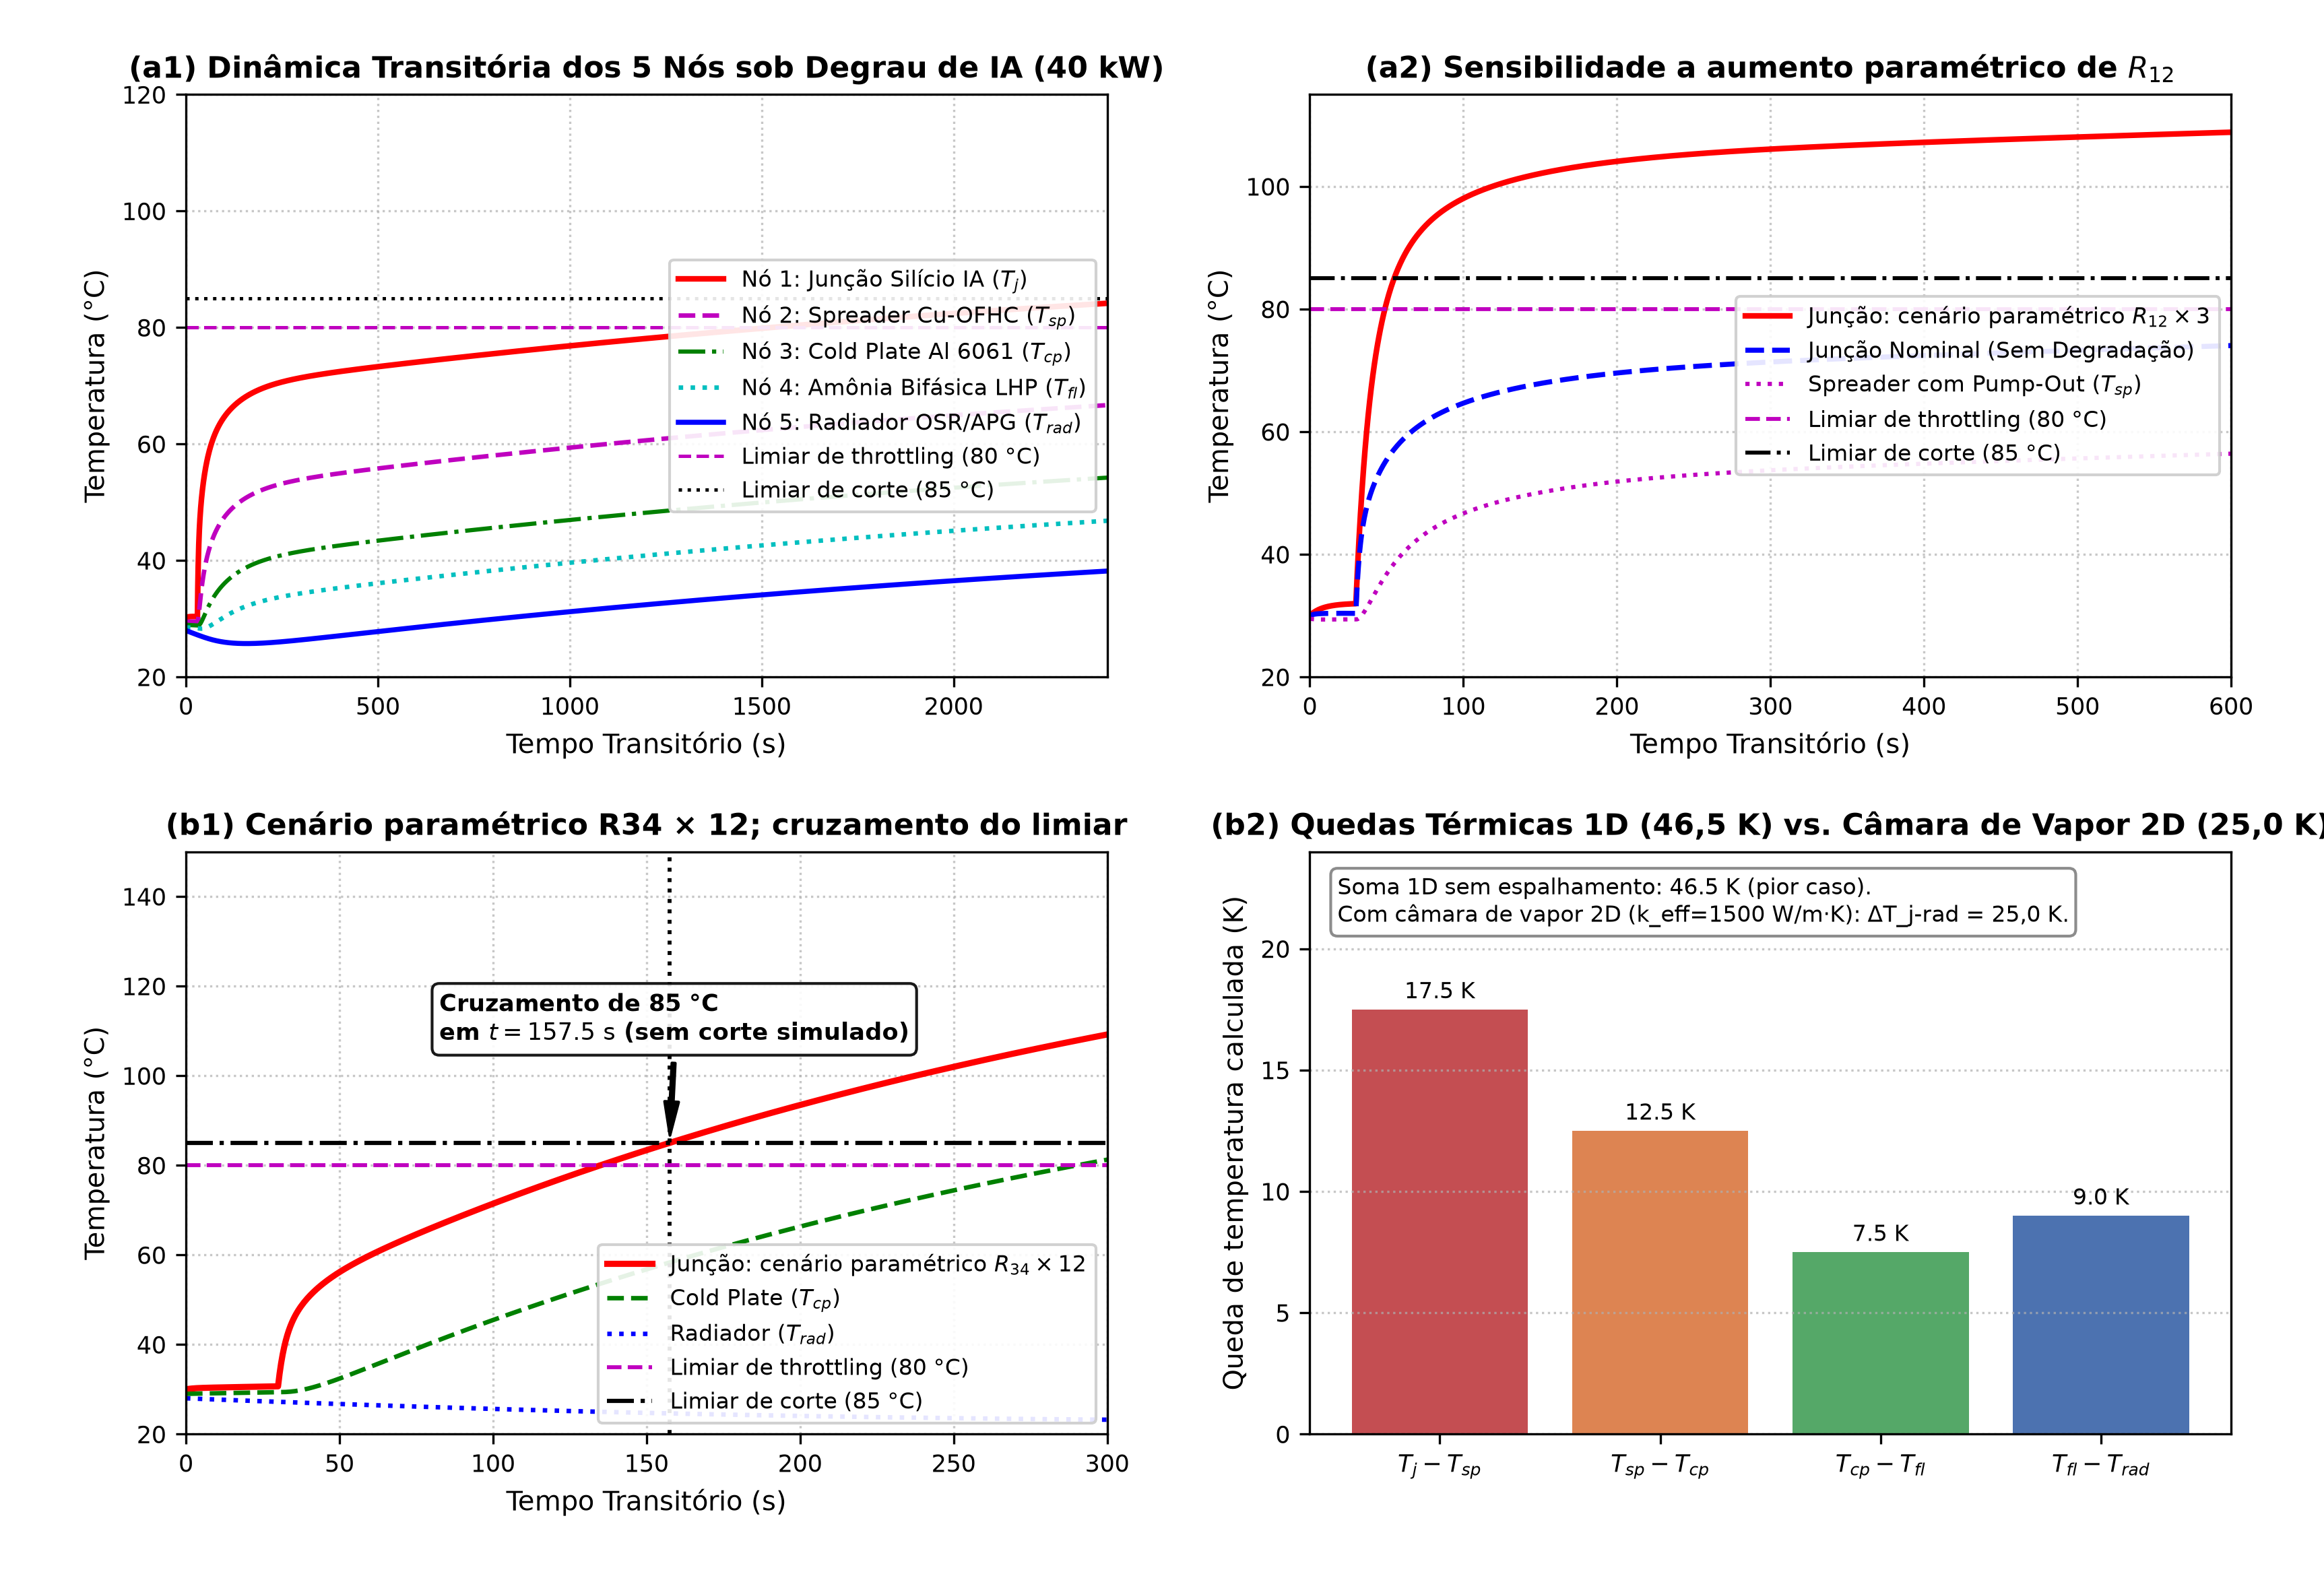
\includegraphics[width=0.82\textwidth]{figuras/figura_4_2_dinamica_rede_nodal_estresse.png}
    \caption{Simulação exploratória em malha aberta da rede nodal com parâmetros provisórios: (a1) degrau imposto de 2 para 40~kW em $t=30$~s; no caso nominal, $T_j$ cruza 80~$^\circ$C em 1256~s e 85~$^\circ$C em 2042{,}5~s, sem que o script aplique throttling ou corte; (a2) sensibilidade a $R_{12}\times3$, com cruzamentos calculados em 49~s e 55~s; (b1) sensibilidade a $R_{34}\times12$, com cruzamentos em 135~s e 157{,}5~s; (b2) contribuição de cada resistência para a queda calculada de 46{,}5~K a 40~kW, incompatível com os 25~K usados no balanço reduzido. Os multiplicadores não foram derivados de ensaios de falha, e a figura não é validação do LHP, do TIM ou do controlador.}
    \label{fig:dinamica_rede_nodal_estresse}
\end{figure}

A leitura da Figura~\ref{fig:dinamica_rede_nodal_estresse} deve permanecer restrita aos parâmetros inseridos no integrador explícito e ao horizonte simulado:
\begin{enumerate}[label=(\alph*)]
    \item \textbf{Caso nominal (Subpainel~a1):} Com o estado inicial imposto e o degrau de 40~kW em $t=30$~s, em $t=600$~s o integrador calcula $T_j=74{,}76^\circ$C, $T_{sp}=57{,}29^\circ$C, $T_{cp}=44{,}90^\circ$C, $T_{fl}=37{,}62^\circ$C e $T_{rad}=29{,}42^\circ$C. A resposta ainda é transitória. Na extensão de 2400~s, a malha aberta cruza 80~$^\circ$C em 1256~s e 85~$^\circ$C em 2042{,}5~s. Como nenhuma ação TEMS ou desligamento é aplicada, a continuação após esses cruzamentos é contrafactual e não demonstra operação segura;
    
    \item \textbf{Sensibilidade de $R_{12}$ (Subpainel~a2):} O multiplicador paramétrico $R_{12}\times3$ cruza 80~$^\circ$C em 49~s e 85~$^\circ$C em 55~s. Esses tempos resultam do integrador e das condições iniciais; não são tempos de falha de um TIM real nem incluem acionamento do controlador;
    
    \item \textbf{Sensibilidade de $R_{34}$ (Subpainel~b1):} O multiplicador $R_{34}\times12$ cruza 80~$^\circ$C em 135~s e 85~$^\circ$C em 157{,}5~s. O script não relaciona esse multiplicador à perda de vazão, ao limite capilar ou ao CHF, e não executa o corte de hardware;
    
    \item \textbf{Reconciliação das resistências (Subpainel~b2):} Para 40~kW atravessando a cadeia, as quedas nos quatro elementos somam 46{,}5~K. Isso não coincide com $\Delta T_{j-rad}=25$~K do modelo concentrado da Figura~\ref{fig:fluxos_orbitais_comparativos}; a diferença permanece aberta até que os parâmetros sejam obtidos para uma arquitetura definida.
\end{enumerate}

\subsection{Modelagem Radiativa e Dimensionamento Óptico do Radiador Espacial}
\label{sec:modelagem_radiador_espacial}

A rejeição térmica de centros de dados espaciais no vácuo apoia-se com exclusividade na radiação superficial para o espaço circundante. Para garantir a rigorosa homogeneidade dimensional e eliminar ambiguidades entre densidade de fluxo ($\text{W/m}^2$) e potência térmica ($\text{W}$), formula-se o balanço térmico radiativo superficial em termos da taxa líquida de calor rejeitado para o espaço ($Q_{net,rej}$, expresso estritamente em Watts):
\begin{equation}
    Q_{net,rej}(t) = Q_{emit}(t) - P_{abs,amb}(t) \quad \text{[W]}
    \label{eq:balanco_liquido_radiador_potencia}
\end{equation}
em que $Q_{emit}(t)$ é a potência térmica bruta emitida pela área ativa do radiador ($A_{rad}$) e $P_{abs,amb}(t)$ é a potência radiativa parasita total absorvida a partir das fontes ambientais externas (Sol, albedo e infravermelho terrestre).

A potência emitida no modelo reduzido de corpo cinzento difuso é calculada em relação ao fundo radiativo ($T_{space}$):
\begin{equation}
    Q_{emit}(t) = \varepsilon_{ir}(t) \cdot \sigma \cdot A_{rad} \cdot \eta_{fin} \cdot \left( T_{rad}^4(t) - T_{space}^4 \right) \quad \text{[W]}
    \label{eq:stefan_boltzmann_radiador_rigoroso}
\end{equation}
onde:
\begin{itemize}[leftmargin=*]
    \item $\sigma = 5{,}67037 \times 10^{-8}\text{ W/(m}^2\text{K}^4)$ é a constante fundamental de Stefan-Boltzmann;
    \item $\varepsilon_{ir}(t)$ é a emissividade hemisférica no infravermelho térmico ($\lambda \approx 4\text{ a }50\ \mu\text{m}$);
    \item $A_{rad}$ é a área superficial total de emissão radiativa livre (para painéis desdobráveis bifaciais com ambas as faces expostas ao espaço, $A_{rad} = 2 A_{painel}$);
    \item $\eta_{fin}$ é a eficiência média de aleta radiativa;
    \item $T_{rad}(t)$ é a temperatura média termodinâmica absoluta da superfície externa do radiador;
    \item $T_{space}=3{,}0\text{ K}$ é a temperatura de fundo usada no termo de emissão. A absorção de IR terrestre e albedo é contabilizada uma única vez em $P_{abs,amb}$, na Equação~(\ref{eq:potencia_parasita_absorvida}); portanto, não se inclui simultaneamente um sumidouro terrestre equivalente em $Q_{emit}$. Esta é uma aproximação de balanço concentrado: a emissão do radiador para o disco terrestre não é modelada como uma rede radiativa própria.
\end{itemize}

A potência ambiental parasita total absorvida ($P_{abs,amb}$) decompõe-se rigorosamente nas áreas projetadas e fatores de forma geométricos:
\begin{align}
    P_{abs,amb}(t) &= \underbrace{\alpha_s(t) \cdot A_{sol,proj}(t) \cdot G_{AM0} \cdot S(t)}_{\text{Absorção Solar Direta}} \nonumber \\
    &\quad + \underbrace{\alpha_s(t) \cdot A_{rad} \cdot F_{rad-E}(h, \phi) \cdot a_E \cdot G_{AM0} \cdot S(t) \cdot \max(0, \cos \theta_{sun,nadir})}_{\text{Absorção de Albedo Terrestre}} \nonumber \\
    &\quad + \underbrace{\varepsilon_{ir}(t) \cdot A_{rad} \cdot F_{rad-E}(h, \phi) \cdot q_{Earth}}_{\text{Absorção Infravermelha Terrestre}} \quad \text{[W]}
    \label{eq:potencia_parasita_absorvida}
\end{align}
onde $A_{sol,proj}(t) = A_{rad} \cdot \max(0, \, \hat{\mathbf{n}}_{rad} \cdot \hat{\mathbf{s}}(t))$ é a área efetiva projetada normal ao vetor solar. Na atitude nominal estática em órbita heliossíncrona *Dawn-Dusk*, a normal do radiador aponta permanentemente para o semiplano anti-solar ($\hat{\mathbf{n}}_{rad} \cdot \hat{\mathbf{s}} \le 0$), anulando $A_{sol,proj} = 0\text{ m}^2$ em regime nominal.

\subsubsection{Condução Bidimensional em Aletas de APG Anisotrópico e Eficiência \texorpdfstring{($\eta_{fin}$)}{(eta_fin)}}

O transporte de calor entre os tubos coletores do condensador bifásico de amônia e as extremidades emissoras do radiador depende da condução sólida bidimensional nas aletas. Diferentemente de metais isotrópicos homogêneos, adota-se uma estrutura avançada de \textbf{Grafite Pirolítico Encapsulado} (\textit{Annealed Pyrolytic Graphite} -- APG). O APG exibe condutividade térmica planar extraordinária no plano basal cristalográfico ($k_{xx} = k_{yy} = k_{in-plane} \ge 1500\text{ W/(m}\cdot\text{K)}$), mas baixa condutividade transversal através das lamelas de grafeno ($k_{zz} = k_{through-plane} \approx 10\text{ W/(m}\cdot\text{K)}$).

Para conferir rigidez estrutural e mitigar a fragilidade mecânica do grafite sob cargas de lançamento, o núcleo de APG de espessura $t_{APG} = 1{,}5\text{ mm}$ é encapsulado em facesheets estruturais de compósito de fibra de carbono de ultra-alto módulo K13D2U em matriz cianato-éster de espessura $t_c = 0{,}25\text{ mm}$ e condutividade $k_c = 600\text{ W/(m}\cdot\text{K)}$. A condutividade térmica efetiva no plano da aleta compósita sanduíche ($k_{eff}$) é calculada pela média ponderada das camadas paralelas:
\begin{align}
    k_{eff} &= \frac{k_{in-plane} t_{APG} + 2 k_c t_c}{t_{APG} + 2 t_c} \nonumber \\
    &= \frac{1500 \cdot 1{,}5 + 2 \cdot 600 \cdot 0{,}25}{2{,}0} = 1275{,}0\text{ W/(m}\cdot\text{K)} \quad \text{[VERIFICÁVEL]}
    \label{eq:condutividade_efetiva_apg}
\end{align}

Considerando uma aleta retangular de comprimento livre $L_{fin} = 75\text{ mm}$ entre tubos condutores de condensação espaçados de $2 L_{fin} = 150\text{ mm}$, a equação diferencial de condução de calor unidimensional em regime permanente ao longo da coordenada longitudinal $x$ da aleta, com emissão radiativa simétrica em ambas as faces para o fundo $T_{space}$, é governada por:
\begin{equation}
    k_{eff} t_{fin} \frac{d^2 T(x)}{dx^2} = 2 \varepsilon_{ir} \sigma \left( T^4(x) - T_{space}^4 \right), \quad 0 \le x \le L_{fin}
    \label{eq:equacao_aleta_nao_linear_exata}
\end{equation}
sujeita às condições de contorno de Dirichlet na raiz condutora e de Neumann (adiabática) na ponta de simetria:
\begin{equation}
    T(0) = T_{root} = 45{,}0^\circ\text{C} = 318{,}15\text{ K}, \qquad \left. \frac{dT}{dx} \right|_{x = L_{fin}} = 0
    \label{eq:condicoes_contorno_aleta}
\end{equation}

Como o gradiente térmico ao longo da aleta de APG é pequeno em virtude de sua elevadíssima condutividade ($k_{eff} = 1275\text{ W/(m}\cdot\text{K)}$), lineariza-se a troca radiativa quártica através da expansão em série de Taylor em torno da temperatura média da raiz ($T_{root}$):
\begin{equation}
    T^4(x)-T_{space}^4 = (T(x)-T_{space})(T(x)+T_{space})(T^2(x)+T_{space}^2) \approx h_{rad}(T(x)-T_{space}), \quad h_{rad}=\varepsilon_{ir}\sigma(T_{root}+T_{space})(T_{root}^2+T_{space}^2)\approx1{,}512\text{ W/(m}^2\text{K)}
    \label{eq:coeficiente_linearizado_hrad}
\end{equation}
A integração analítica fechada da equação diferencial linearizada resulta no perfil hiperbólico de temperatura $\theta(x) = \theta_{root} \cosh[m (L_{fin} - x)] / \cosh(m L_{fin})$, definindo a eficiência de aleta radiativa ($\eta_{fin}$):
\begin{equation}
    \eta_{fin,ideal} = \frac{\tanh(m L_{fin})}{m L_{fin}}, \qquad m = \sqrt{\frac{2 h_{rad}}{k_{eff} t_{fin}}} = \sqrt{\frac{2 \cdot 1{,}512}{1275 \cdot 0{,}0020}} \approx 1{,}089\text{ m}^{-1}
    \label{eq:eficiencia_aleta_apg_rigorosa}
\end{equation}
Para $L_{fin} = 0{,}075\text{ m}$, tem-se $m L_{fin} = 0{,}1683$, resultando em uma eficiência excepcional de:
\begin{equation}
    \eta_{fin,ideal} = \frac{\tanh(0{,}0817)}{0{,}0817} \approx \mathbf{0{,}9978} \quad (> 99\%)
\end{equation}
O valor $\eta_{fin}=0{,}945$ empregado no script é uma premissa de projeto [PROVISÓRIA]; não há modelo de contato ou ensaio no repositório que demonstre que essa margem represente perdas reais. A eficiência ideal calculada da aleta e o fator efetivo usado no balanço devem, portanto, permanecer identificados separadamente.

\subsubsection{Modelo Dinâmico de Degradação Óptica Temporal (BOL para EOL em 10 Anos)}

As propriedades termo-ópticas dos revestimentos externos degradam-se de forma não linear ao longo dos 10 anos de vida útil de projeto, em decorrência do escurecimento fotoquímico sob radiação ultravioleta do vácuo cósmico (\textit{vacuum UV solar browning}), impactos de oxigênio atômico (AO) e deposição de filmes moleculares desgaseificados da espaçonave (\textit{molecular contamination outgassing}). Rejeita-se a soma estática de constantes arbitrárias e adota-se o modelo físico de evolução temporal por saturação exponencial, recomendado pela norma ECSS-E-HB-31-01 Parte 6:
\begin{equation}
    \alpha_s(t) = \alpha_{s,BOL} + \left( \alpha_{s,EOL} - \alpha_{s,BOL} \right) \left[ 1 - \exp\left( -\frac{t}{\tau_{deg}} \right) \right]
    \label{eq:lei_degradacao_optica_temporal}
\end{equation}
onde:
\begin{itemize}[leftmargin=*]
    \item Para os **Espelhos Ópticos Solares de Quartzo/Prata (OSR)** aplicados sobre os radiadores térmicos: $\alpha_{s,BOL} = 0{,}08$, saturando em $\alpha_{s,EOL} = 0{,}14$ em 10 anos, com constante de tempo de saturação por radiação UV $\tau_{deg,OSR} = 3{,}2\text{ anos}$. A emissividade térmica no infravermelho mantém-se praticamente inalterada e estável em $\varepsilon_{ir} = 0{,}88 \pm 0{,}01$, pois o quartzo fundido é inerte à erosão por AO;
    \item Para a **Tinta Branca Cerâmica de Silicato (AZ-93)** empregada na carcaça estrutural externa: $\alpha_{s,BOL} = 0{,}15$, degradando para $\alpha_{s,EOL} = 0{,}26$, com constante de tempo $\tau_{deg,AZ} = 2{,}1\text{ anos}$ e $\varepsilon_{ir} = 0{,}91 \rightarrow 0{,}89$.
\end{itemize}

O impacto térmico direto dessa degradação sobre o radiador na órbita heliossíncrona reside no aumento de $+75\%$ na absortividade solar ($\Delta \alpha_s = +0{,}06$). Como a atitude nominal é anti-solar, a absorção de albedo terrestre residual (Eq.~\ref{eq:potencia_parasita_absorvida}) cresce ligeiramente de $2{,}17\text{ W/m}^2$ para $3{,}80\text{ W/m}^2$. A elevação efetiva de temperatura de equilíbrio da carcaça do satélite ao longo da década situa-se em $\Delta T_{eq} \approx +3{,}8\text{ K}$ na atitude nominal, e alcança $+12\text{ a }+16\text{ K}$ apenas se houver exposição solar direta de faces estruturais revestidas com AZ-93.

\subsubsection{Sensibilidade Térmica a Desvios de Atitude e Análise de Margem Operacional}

Para substituir noções imprecisas de ``saturação anti-solar'', modela-se rigorosamente o impacto térmico de um \textbf{desvio angular de atitude} ($\delta \theta_{att}$) do sistema de controle de atitude (ADCS) em relação ao vetor anti-solar ideal. Se a plataforma sofrer uma perturbação de guinada ou arfagem de magnitude $\delta \theta_{att}$, a face do radiador deixa de estar na sombra do corpo principal e passa a interceptar radiação solar direta com área projetada $A_{sol,proj} = A_{rad} \sin |\delta \theta_{att}|$.

A densidade de fluxo solar direto incidente absorvido passa a ser:
\begin{equation}
    q_{sol,abs,pert}(t) = \alpha_{s}(t) \cdot G_{AM0} \cdot \sin |\delta \theta_{att}|
    \label{eq:fluxo_solar_perturba_atitude}
\end{equation}
Para um desvio angular $|\delta \theta_{att}|$ sob as propriedades EOL assumidas no script ($\alpha_{s,EOL}=0{,}24$):
\begin{equation}
    q_{sol,abs,pert} = \alpha_{s,EOL} G_{AM0} \sin(|\delta\theta_{att}|)
\end{equation}
Para $A_{rad}=88{,}6\text{ m}^2$, $Q_{int}=41{,}984\text{ kW}$, $\varepsilon_{ir,EOL}=0{,}82$, $\eta_{fin}=0{,}945$ e o fluxo ambiental médio SSO calculado de $52{,}48\text{ W/m}^2$, o modelo prevê, já em $\delta\theta=0^\circ$, $T_{rad}=57{,}68^\circ\text{C}$ e $T_j=82{,}68^\circ\text{C}$ usando $\Delta T_{j-rad}=25\text{ K}$ [PROVISÓRIO]. Isso supera o teto de $55^\circ\text{C}$ do radiador e a meta de throttling de $80^\circ\text{C}$. O limiar de $85^\circ\text{C}$ é alcançado pelo modelo perto de $2{,}62^\circ$ de desvio. A área de sensibilidade de $92{,}0\text{ m}^2$ resulta em $T_{rad}=54{,}89^\circ\text{C}$ e $T_j=79{,}89^\circ\text{C}$ nas mesmas condições; ela não substitui o dimensionamento de EOL com perdas e incertezas fechadas.

A Tabela~\ref{tab:dimensionamento_radiador_comparativo} registra os resultados reproduzíveis do modelo reduzido. O script calcula fluxos para SSO e LEO; embora calcule o período orbital GEO, não calcula para GEO a sombra, os fluxos absorvidos ou o balanço térmico. Os valores de área abaixo são estimativas condicionais em equilíbrio, não qualificação de projeto.

\begin{table}[!ht]
\centering
\small
\renewcommand{\arraystretch}{0.85}
\caption{Resultados do balanço radiativo EOL adotado para SSO e LEO. Os valores GEO não são calculados pelo script atual.}
\label{tab:dimensionamento_radiador_comparativo}
\resizebox{0.95\textwidth}{!}{%
\begin{tabular}{lcccc}
\hline
\textbf{Parâmetro de Dimensionamento Radiativo} & \textbf{SSO Dawn-Dusk (700 km)} & \textbf{LEO Convencional (500 km)} & \textbf{GEO (35.786 km)} & \textbf{Classificação Epistêmica} \\ \hline
Potência térmica de entrada usada ($Q_{int}$) & $41{,}984\text{ kW}$ & $41{,}984\text{ kW}$ & -- & \textbf{[ENTRADA DO SCRIPT]} Rastrear com o balanço elétrico do nó \\
Fator de visão radiador--Terra ($F_{rad-E}$) & $0{,}2328$ & $0{,}4473$ & -- & \textbf{[CALCULADO]} GEO ainda não avaliado radiativamente \\
Fluxo parasita médio ($q_{parasita}$) & $52{,}48\text{ W/m}^2$ & $97{,}95\text{ W/m}^2$ (pico $194{,}88$) & -- & \textbf{[CALCULADO]} Média orbital do script; LEO é transiente \\
Emissão no limite $T_{rad}=55^\circ$C & $509{,}50\text{ W/m}^2$ & $509{,}50\text{ W/m}^2$ & $509{,}50\text{ W/m}^2$ & \textbf{[CALCULADO]} $\varepsilon_{EOL}\sigma\eta_{fin}(T_{rad}^4-T_{space}^4)$ \\
Capacidade líquida em $55^\circ$C ($q_{net,rej}$) & $457{,}02\text{ W/m}^2$ & $411{,}55\text{ W/m}^2$ (média) & -- & \textbf{[CALCULADO]} Não inclui margem de incerteza \\
Área de equilíbrio requerida a $55^\circ$C & $91{,}86\text{ m}^2$ & $102{,}02\text{ m}^2$ (média) & -- & \textbf{[CALCULADO]} $Q_{int}/q_{net,rej}$; LEO não é sizing dinâmico \\
Área adotada no caso SSO & $88{,}6\text{ m}^2$ & -- & -- & \textbf{[PREMISSA DE PROJETO]} Resultado: $T_{rad}=57{,}68^\circ$C, $T_j=82{,}68^\circ$C \\ \hline
\end{tabular}%
}
\end{table}

A avaliação atual compara fluxos orbitais em SSO e LEO. Para o caso EOL modelado, o fluxo parasita médio é $52{,}48\text{ W/m}^2$ em SSO e $97{,}95\text{ W/m}^2$ em LEO, com pico orbital LEO de $194{,}88\text{ W/m}^2$. Esses valores dependem da geometria e das propriedades termo-ópticas assumidas. O script não calcula balanço radiativo GEO; portanto, não se apresenta comparação térmica de três órbitas nem se afirma dimensionamento GEO.

A síntese dos fluxos ambientais SSO/LEO e da sensibilidade do equilíbrio térmico ao erro de atitude é apresentada na Figura~\ref{fig:fluxos_orbitais_comparativos}.

\begin{figure}[htbp]
    \centering
    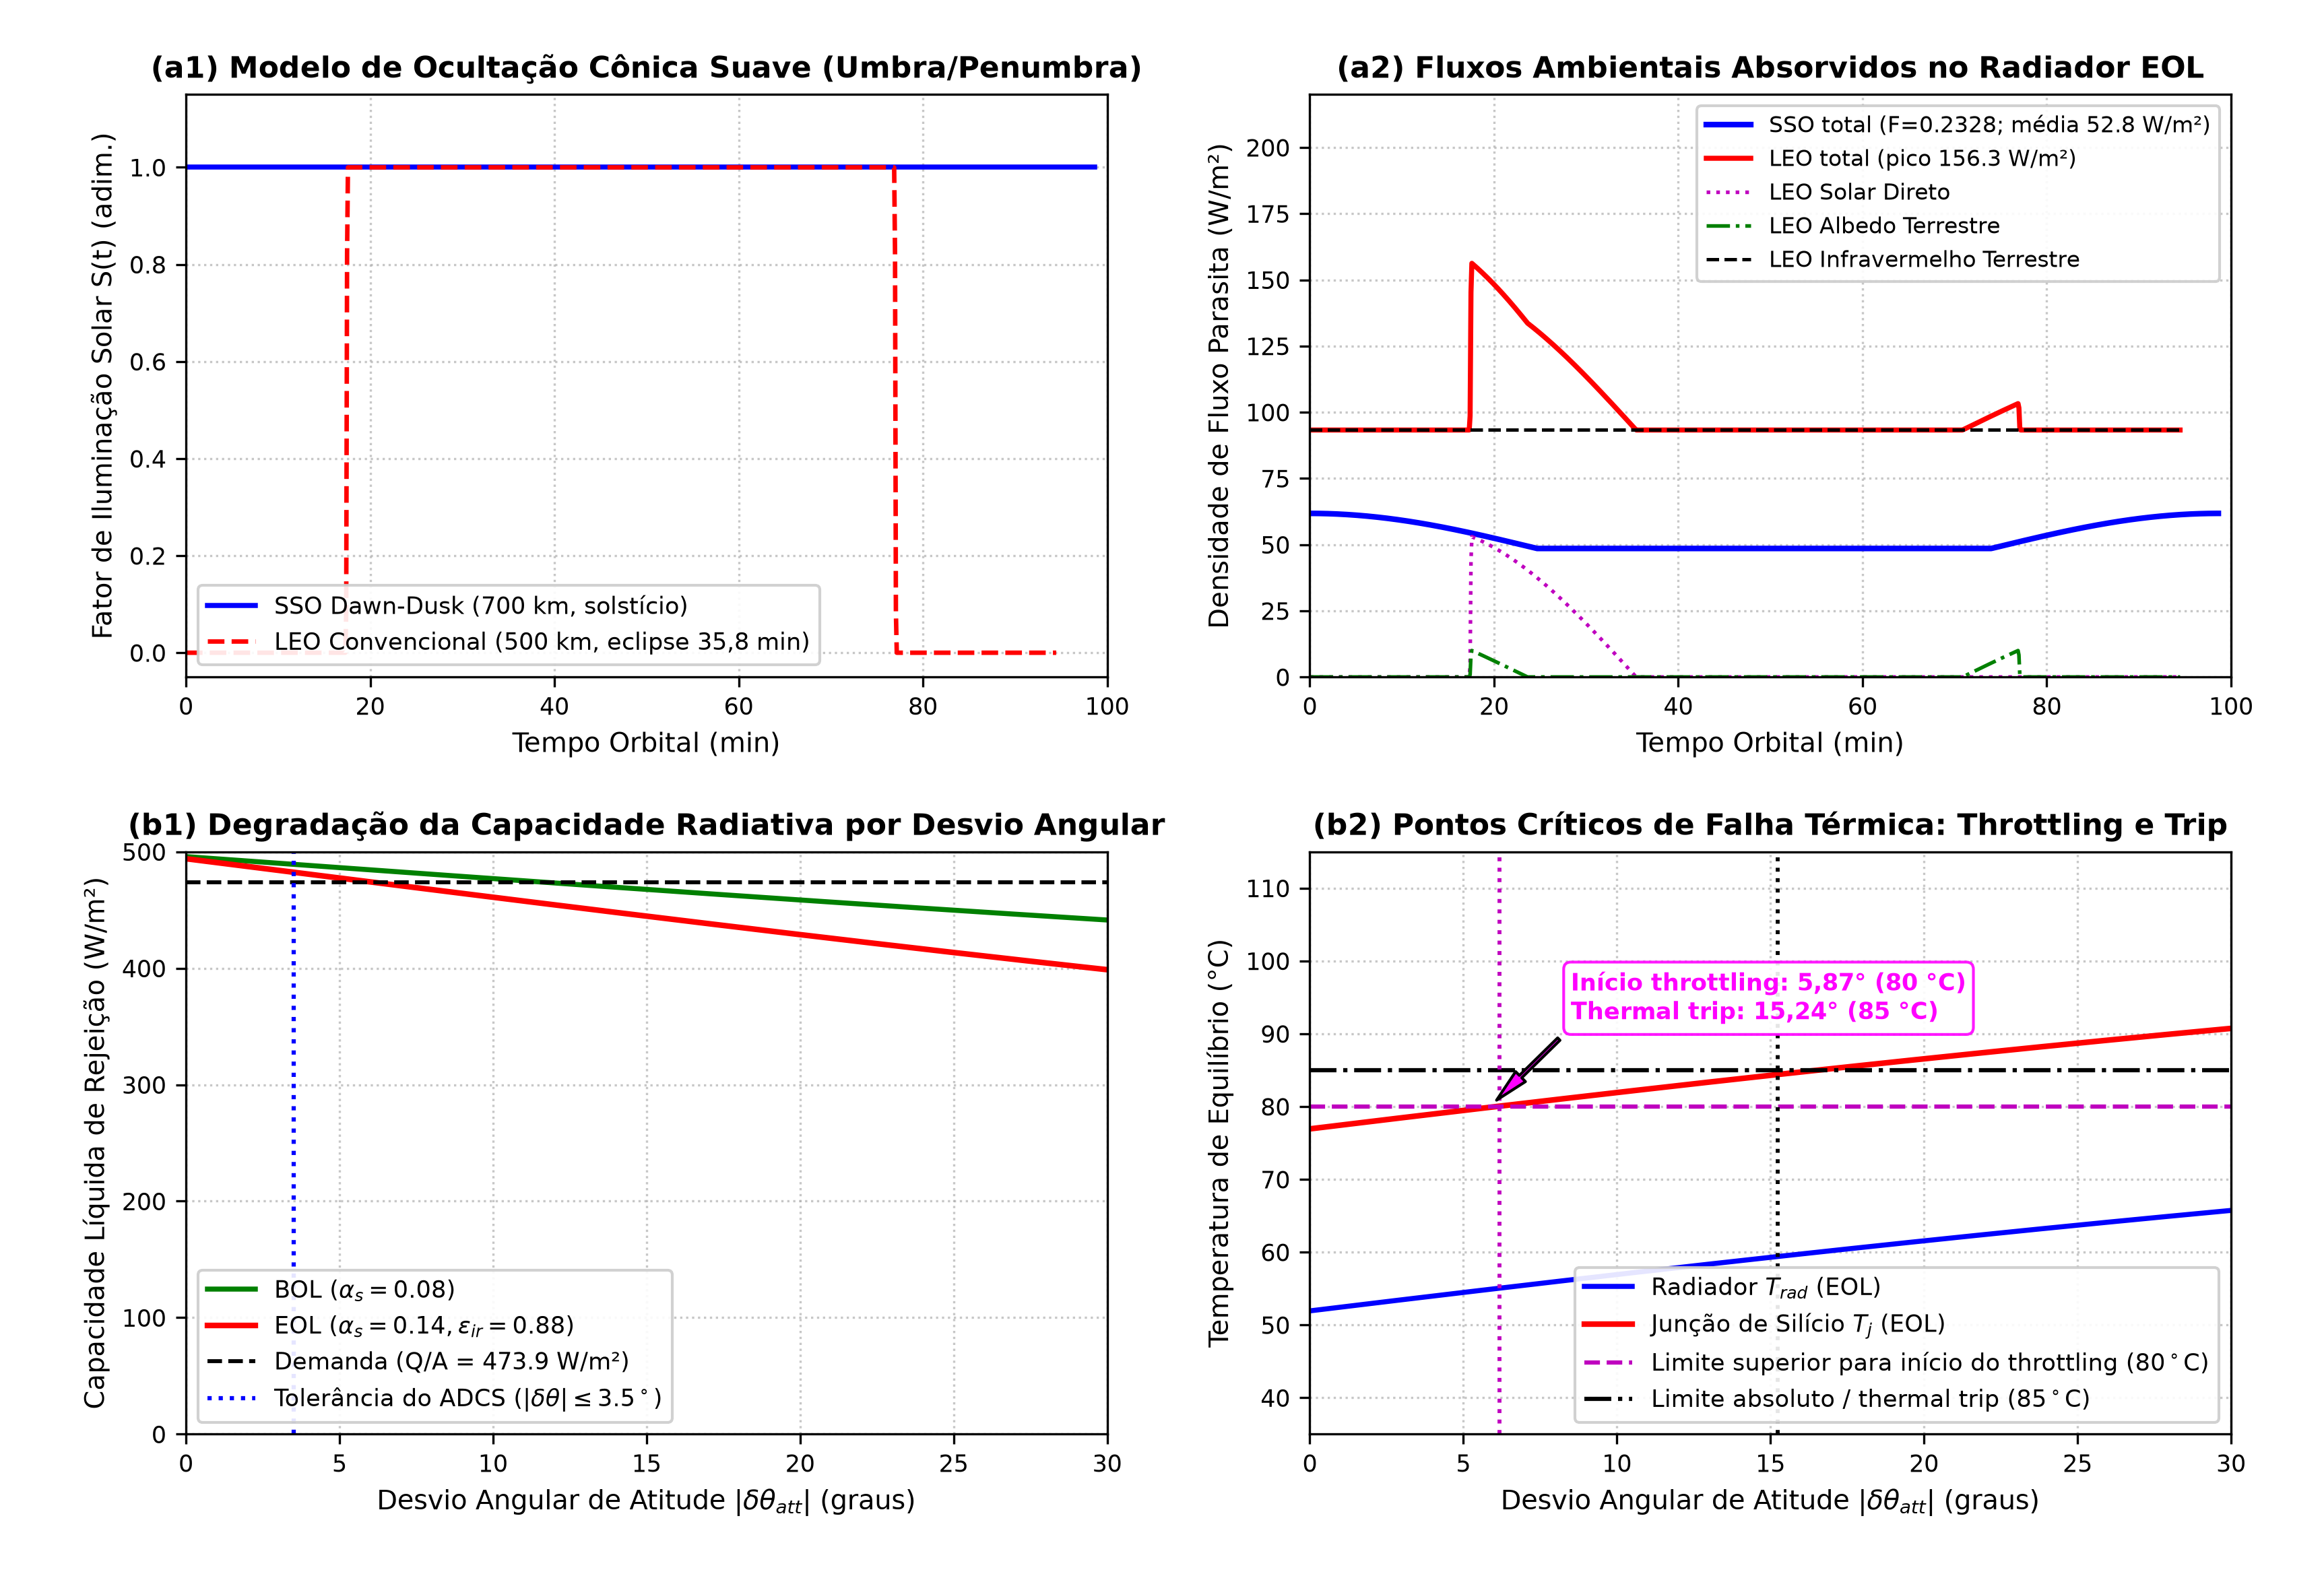
\includegraphics[width=0.82\textwidth]{figuras/figura_4_1_fluxos_orbitais_comparativos.png}
    \caption{Modelo radiativo reduzido para SSO e LEO: (a1) fator de iluminação em uma revolução, com eclipse LEO; (a2) fluxos ambientais absorvidos usando propriedades EOL assumidas; (b1) capacidade líquida de rejeição em função do erro de atitude, comparada à demanda térmica; (b2) temperaturas de equilíbrio do radiador e da junção, com o limite de início de throttling em $80^\circ$C e o limite absoluto em $85^\circ$C. O SSO nominal já excede $80^\circ$C no caso EOL calculado. GEO não é simulado nesta figura.}
    \label{fig:fluxos_orbitais_comparativos}
\end{figure}

A decomposição dos quatro subpainéis da Figura~\ref{fig:fluxos_orbitais_comparativos} evidencia:
\begin{enumerate}[label=(\alph*)]
    \item \textbf{Iluminação orbital (Subpainel~a1):} O cenário LEO de 500~km e $\beta=20^\circ$ produz eclipse de cerca de $35{,}8$~min por revolução no modelo cônico. O SSO a $700$~km e $\beta=85^\circ$ não apresenta eclipse no ciclo nominal representado; a figura não calcula a evolução sazonal anual de $\beta$;
    
    \item \textbf{Fluxos ambientais (Subpainel~a2):} Para SSO, $F_{rad-E}=0{,}2328$, o albedo médio absorvido calculado é $7{,}25\text{ W/m}^2$ e o IR terrestre absorvido é $45{,}23\text{ W/m}^2$, totalizando $52{,}48\text{ W/m}^2$. Para LEO, o script calcula média de $97{,}95\text{ W/m}^2$ e pico de $194{,}88\text{ W/m}^2$. São resultados de uma órbita e das propriedades EOL provisórias, não uma caracterização anual;
    
    \item \textbf{Margem térmica e erro de atitude (Subpainéis~b1/b2):} Com $A_{rad}=88{,}6\text{ m}^2$, a demanda $Q_{int}/A_{rad}=473{,}86\text{ W/m}^2$ já excede a capacidade líquida do caso SSO em $55^\circ$C ($457{,}02\text{ W/m}^2$). O equilíbrio nominal calculado é $T_{rad}=57{,}68^\circ$C e $T_j=82{,}68^\circ$C; assim, a condição já requer throttling antes de qualquer erro de atitude. O limite de $85^\circ$C é alcançado perto de $2{,}62^\circ$ de desvio no modelo; o limiar de trip é $85^\circ$C, não $105^\circ$C;
    
    \item \textbf{Área condicional e escopo GEO:} A $55^\circ$C, o modelo requer $91{,}86\text{ m}^2$ em SSO e $102{,}02\text{ m}^2$ em LEO se usado o fluxo LEO médio; o cálculo não incorpora a resposta térmica transiente nem margem de incerteza. A área SSO adotada de $88{,}6\text{ m}^2$ é insuficiente para a carga térmica usada. O código atual não calcula os fluxos ou a área GEO.
\end{enumerate}

\subsection{Dinâmica de Co-Design Eletrotérmico de Chips de IA e Condição Analítica de Instabilidade}
\label{sec:co_design_eletrotermico_runaway}

A modelagem térmica no nível de silício exige a integração acoplada entre o comportamento elétrico dos circuitos semicondutores e a dinâmica de transferência de calor. Em nós litográficos avançados com transistores FinFET e Gate-All-Around (GAA) sub-7~nm, a elevação da temperatura de junção ($T_j$) induz o aumento exponencial das correntes térmicas de fuga quântica e termoiônica. Esse acoplamento eletrotérmico bidirecional estabelece uma retroalimentação não linear que, na ausência de capacidade adequada de extração térmica, pode deflagrar a divergência térmica descontrolada (\textit{thermal runaway}).

\subsubsection{Fronteira de Potência no Nó e Decomposição da Dissipação}

Para evitar duplicidade com os modelos do Capítulo~\ref{sec:arquitetura_barramento_balanco}, a potência entregue ao nó ($P_{node}$) decompõe-se em:
\begin{equation}
    P_{node}(t) = \underbrace{P_{core}(t) + P_{mem}(t)}_{P_{chip}(t)} + P_{VRM}(t) + P_{interconnect}(t) \quad \text{[W]}
    \label{eq:decomposicao_potencia_no}
\end{equation}
sendo $P_{chip}$ a dissipação nos aceleradores de IA (núcleos e memórias HBM3e em interposer CoWoS), $P_{VRM} \approx 2{,}3\text{ kW}$ as perdas dos conversores GaN PoL ($\eta_{PoL} \approx 94{,}5\%$), e $P_{interconnect} \approx 650\text{ W}$ a potência de barramentos PCIe 5.0/CXL e roteadores ópticos.

A potência do acelerador neural decompõe-se na componente dinâmica e na fuga sublimiar:
\begin{equation}
    P_{chip}(V_{core}, f_{clk}, T_j) = P_{dyn}(V_{core}, f_{clk}) + P_{leak}(T_j, V_{core}) \quad \text{[W]}
    \label{eq:potencia_total_chip_rigorosa}
\end{equation}
com potência dinâmica calibrada por $P_{dyn} = (\alpha_{act} C_{eff}) V_{core}^2 f_{clk}$, em que $(\alpha_{act} C_{eff})_{inf} \approx 171{,}0\text{ nF}$ para inferência e $334{,}4\text{ nF}$ para treinamento denso, operando em $V_{core} \in [0{,}65, 1{,}05]\text{ V}$ e $f_{clk} \in [1{,}0, 1{,}8]\text{ GHz}$.

\subsubsection{Modelo de Corrente de Fuga e Estabilidade Térmica (Thermal Runaway)}

A corrente de fuga sublimiar é modulada termicamente por emissão termoiônica e tunelamento quântico (formulação BSIM detalhada no Apêndice~B.7). Para processamento em tempo real, adota-se a formulação empírica calibrada:
\begin{equation}
    P_{leak}(T_j, V_{core}) = P_{leak,ref}(V_{core}) \cdot \exp\left[ \beta_T \left( T_j - T_{ref} \right) \right] \quad \text{[W]}
    \label{eq:potencia_fuga_calibrada_local}
\end{equation}
com $P_{leak,ref}(V_{core}) = I_{leak,ref} V_{core} (V_{core}/V_{core,nom})^2$, sendo $\beta_T = 0{,}0285\text{ K}^{-1}$ [PROVISÓRIO].

A estabilidade de equilíbrio de primeira ordem ($P_{chip}(T_j^*) = \dot{Q}_{out}(T_j^*)$) sob extração $\dot{Q}_{out} = (T_j - T_{sink})/R_{th,j-sink}$ com dependência de transporte capilar $R_{th,j-sink}(Q) = R_{th,0} [1 + (Q/Q_{max,cap})^4]$ impõe a condição estrita de Lyapunov para amortecimento:
\begin{equation}
    \left. \frac{\partial P_{chip}}{\partial T_j} \right|_{T_j^*} < \left. \frac{d\dot{Q}_{out}}{dT_j} \right|_{T_j^*} = \frac{1/R_{th}}{1+\frac{(T_j^*-T_{sink})}{R_{th}^{2}}\left.\frac{dR_{th}}{d\dot Q_{out}}\right|_*} \quad \text{[DEPENDENTE DO MODELO]}
    \label{eq:criterio_estabilidade_box}
\end{equation}
Para as condições nominais ($T_j^* = 70^\circ\text{C}$, $V_{core} = 0{,}85\text{ V}$, $P_{leak} \approx 3{,}6\text{ kW}$), o gradiente de fuga é $\partial P_{leak}/\partial T_j = \beta_T P_{leak} \approx 102{,}6\text{ W/K}$, muito inferior à condutância nominal agregada de $860{,}2\text{ W/K}$ (80 dies em paralelo), garantindo estabilidade. Sob falha severa ($R_{th}$ elevado para $\ge 0{,}35\text{ K/W}$ por degradação de TIM ou dry-out), a condutância cai para $\le 228{,}5\text{ W/K}$. Caso $T_j$ atinja $95^\circ\text{C}$ ($P_{leak} \approx 7{,}4\text{ kW}$), o gradiente sobe para $210{,}9\text{ W/K}$, aproximando-se do limiar de bifurcação de \textit{thermal runaway}.

A violação do envelope de temperatura deflagra as proteções: (a) \textit{thermal throttling} gradual antes de $80^\circ\text{C}$ (reduzindo $f_{clk}$ de $1{,}8$ para $1{,}0\text{ GHz}$); (b) \textit{thermal trip} rígido em $T_{crit} = 85{,}0^\circ\text{C}$ para modo seguro. A Figura~\ref{fig:estabilidade_runaway_lhp} ilustra o crescimento exponencial da fuga, a bifurcação de runaway sob tensão turbo ($1{,}05\text{ V}$) e o mapa de estabilidade no plano $V_{core} \times R_{th,crit}$.

\begin{figure}[htbp]
    \centering
    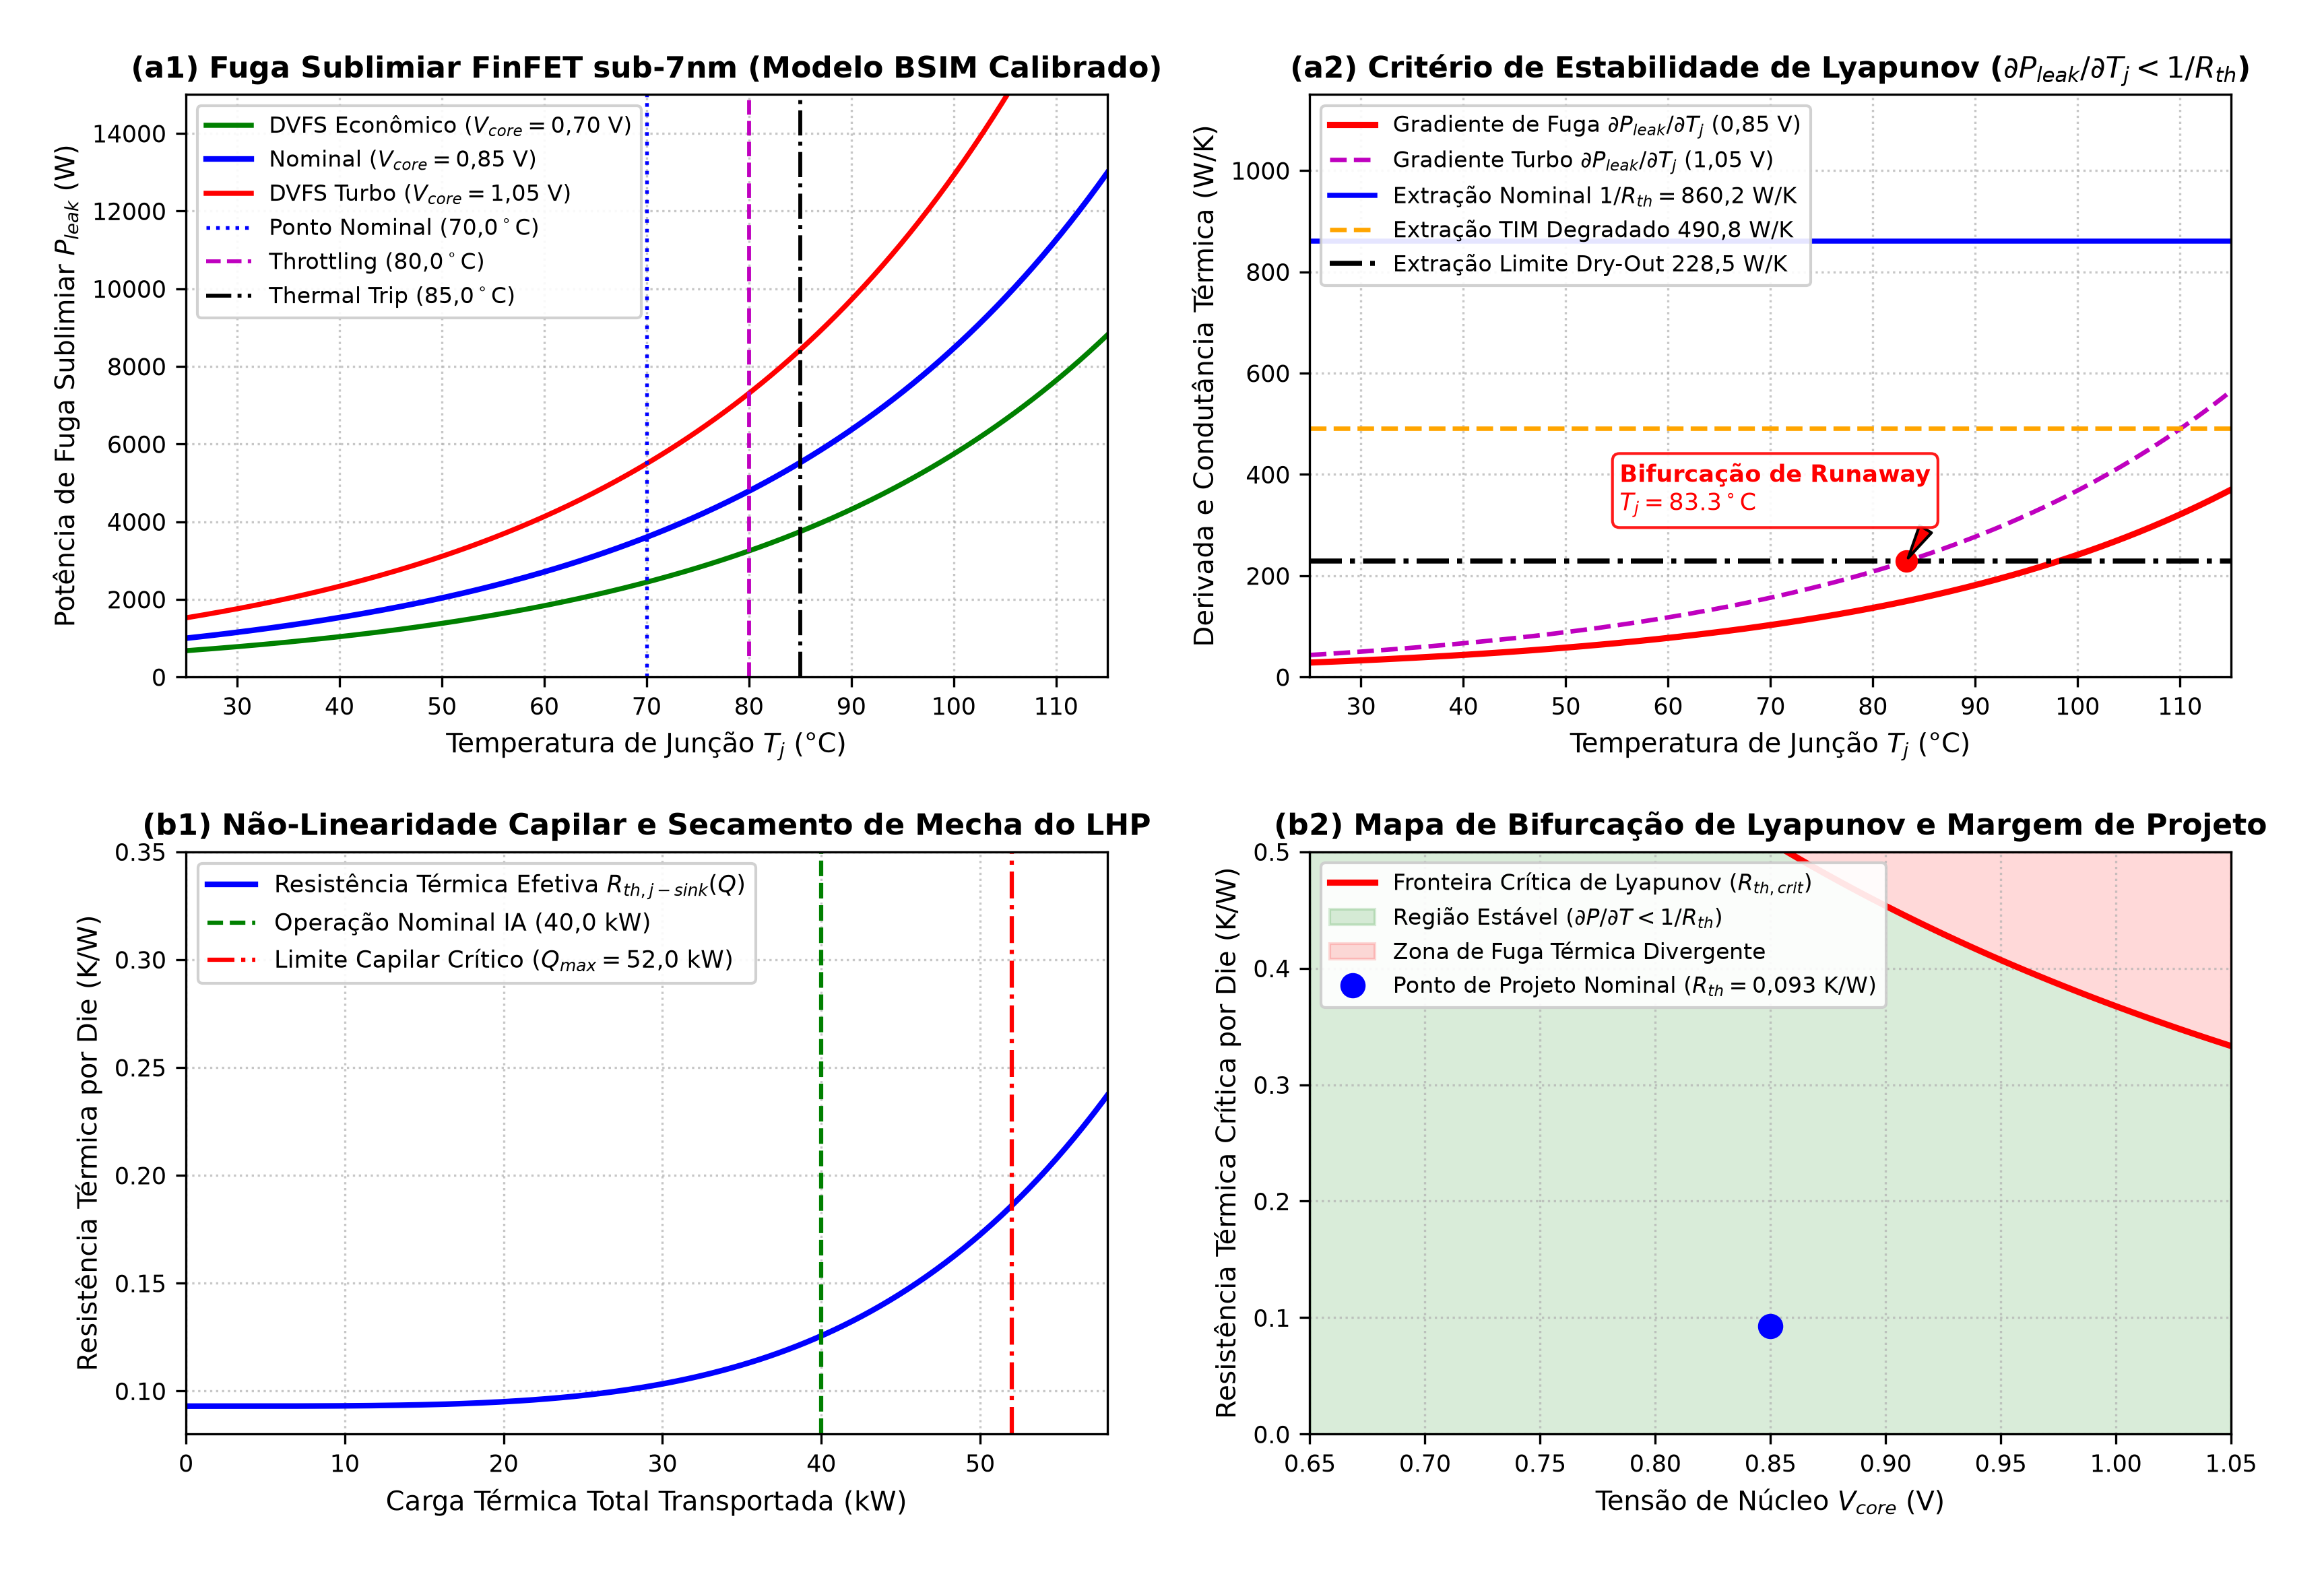
\includegraphics[width=0.82\textwidth]{figuras/figura_4_3_estabilidade_runaway_lhp.png}
    \caption{Co-design eletrotérmico e estabilidade de Lyapunov: (a1) fuga sublimiar calculada por modelo BSIM em função de $T_j$; (a2) critério de Lyapunov identificando bifurcação de runaway a $83{,}4^\circ\text{C}$ sob tensão turbo ($1{,}05\text{ V}$) e extração WCA; (b1) não linearidade da resistência do LHP governada pela aproximação quártica a $Q_{max} = 52{,}0\text{ kW}$; (b2) mapa de bifurcação no plano $V_{core} \times R_{th,crit}$, confirmando que o ponto nominal opera no interior da região estável.}
    \label{fig:estabilidade_runaway_lhp}
\end{figure}

\subsection{Sistema de Gerenciamento Térmico-Energético Ativo (TEMS)}
\label{sec:tems_arquitetura_controle}

Para prevenir que o sistema atinja limiares críticos de instabilidade térmica, minimizar as oscilações mecânicas de fadiga cíclica nas soldas e otimizar dinamicamente a entrega de processamento neural frente à geração solar orbitária e à carga da bateria, desenvolve-se a arquitetura de controle hierárquico em duas camadas do \textbf{Sistema de Gerenciamento Térmico-Energético Ativo} (\textit{Thermal and Energy Management System} -- TEMS).

\subsubsection{Classificação Epistêmica dos Limiares Operacionais de Projeto}

Para eliminar arbitrariedades de parametrização e fornecer rastreabilidade física de engenharia, a Tabela~\ref{tab:classificacao_limiares_tems} cataloga os limiares de controle, segurança e atuação do TEMS sob rigorosa classificação epistêmica.

\begin{table}[!ht]
\centering
\small
\renewcommand{\arraystretch}{0.85}
\caption{Classificação epistêmica e justificativa dos limiares operacionais do TEMS.}
\label{tab:classificacao_limiares_tems}
\resizebox{0.95\textwidth}{!}{%
\begin{tabular}{lcccc}
\hline
\textbf{Limiar / Parâmetro Operacional} & \textbf{Símbolo} & \textbf{Valor de Projeto} & \textbf{Classificação} & \textbf{Justificativa Física / Referência de Norma} \\ \hline
Temperatura Alvo em Regime Normal & $T_{target}$ & $75{,}0^\circ\text{C}$ ($348{,}15\text{ K}$) & \textbf{[REQUISITO DE PROJETO]} & Limite informado para operação normal \\
Limite para Início de Throttling & $T_{thr}<80^\circ\text{C}$ & Antes de $80^\circ\text{C}$ & \textbf{[REQUISITO DE PROJETO]} & Setpoint numérico ainda não definido \\
Temperatura de Corte para Modo Seguro (Thermal Trip) & $T_{crit}$ & $85{,}0^\circ\text{C}$ ($358{,}15\text{ K}$) & \textbf{[REQUISITO DE PROJETO]} & Limite definido para este estudo; não é alegação de limite JEDEC \\
Temperatura Máxima da Bateria BESS & $T_{bat,max}$ & $+35{,}0^\circ\text{C}$ ($308{,}15\text{ K}$) & \textbf{[REQUISITO DE PROJETO]} & Limite definido para este estudo \\
Temperatura Mínima da Bateria BESS & $T_{bat,min}$ & $+10{,}0^\circ\text{C}$ ($283{,}15\text{ K}$) & \textbf{[REQUISITO DE PROJETO]} & Limite definido para este estudo \\
Estado de Carga Mínimo & $SoC_{min}$ & $20{,}0\%$ & \textbf{[REQUISITO DE PROJETO]} & Equivale a $DoD\le80\%$ sob a mesma referência energética \\
Taxa Máxima de Variação de Frequência & $\Delta f_{slew,max}$ & $100{,}0\text{ MHz/s}$ & \textbf{[PROVISÓRIO]} & Limita choque térmico nas esferas de solda BGA \\
Temperatura Máxima do Radiador & $T_{rad,max}$ & $55{,}0^\circ\text{C}$ & \textbf{[REQUISITO DE PROJETO]} & Limite informado para o radiador \\
Banda de Histerese Térmica Anti-Chattering & $\Delta T_{hyst}$ & $3{,}0^\circ\text{C}$ & \textbf{[PROVISÓRIO]} & Amortece comutações espúrias de alta frequência \\ \hline
\end{tabular}%
}
\end{table}

\subsubsection{Camada Rápida Descentralizada: DVFS em Malha Fechada}

A camada rápida atua em nível de die semicondutor e conversores GaN PoL de ponto de carga com período de amostragem de controle sub-milissegundo ($\Delta t_{fast} \le 1{,}0\text{ ms}$). O seu objetivo primário é conter excursões térmicas de alta frequência provocadas por degraus de ativação de tensores lógicos.

A lei de atuação do DVFS modula o vetor de ponto operacional $u_{fast}[k] = [f_{clk}[k], V_{core}[k]]^T$ a partir da leitura filtrada dos diodos térmicos internos do die ($T_j$), seguindo a relação de mapeamento de tensão-frequência do fabricante ($V_{core} = V_{core,min} + \lambda_{DVFS} (f_{clk} - f_{clk,min})$). Para evitar instabilidades de ciclo limite e chaveamento espúrio (\textit{chattering}), implementa-se uma banda de histerese finita com dois limiares desacoplados:
\begin{equation}
    f_{clk}[k] = 
    \begin{cases}
        \max\left( f_{clk,min}, \, f_{clk}[k-1] - \Delta f_{step} \right), & \text{se } T_j[k] \ge T_{thr}, \quad T_{thr}<80^\circ\text{C} \\[0.2cm]
        \min\left( f_{clk,max}, \, f_{clk}[k-1] + \Delta f_{step} \right), & \text{se } T_j[k] \le T_{thr} - \Delta T_{hyst} \\[0.2cm]
        f_{clk}[k-1], & \text{se } T_{thr} - \Delta T_{hyst} < T_j[k] < T_{thr}
    \end{cases}
    \label{eq:dvfs_histerese_antichattering}
\end{equation}
em que o passo discreto de modulação de frequência é restrito pelo limitador de taxa (\textit{slew rate limiter}) para mitigar fadiga por choque mecânico nas soldas:
\begin{equation}
    \Delta f_{step} \le \Delta f_{slew,max} \cdot \Delta t_{fast} = 100\text{ MHz/s} \cdot 10^{-3}\text{ s} = 100\text{ kHz por ciclo}
\end{equation}

A resposta do DVFS não acarreta a paralisação abrupta ou colapso a zero do processamento, mas sim uma \textbf{redução temporária controlada de frequência} (reduzindo a dissipação dinâmica proporcionalmente a $f_{clk}$ e quadraticamente com $V_{core}$), preservando a integridade física e mantendo a vazão computacional no maior patamar compatível com a capacidade instantânea de resfriamento.

\subsubsection{Camada Lenta Supervisória Preditiva: Formulação NMPC com Consciência Orbital}

A camada supervisória do TEMS opera a uma taxa de amostragem de $\Delta t_{ctrl} = 3{,}0\text{ s}$, formulando o problema de controle sob a metodologia de \textbf{Controle Preditivo Baseado em Modelo Não Linear} (\textit{Nonlinear Model Predictive Control} -- NMPC) com horizonte de predição de $N_p = 20$ passos ($60\text{ segundos}$ à frente) e horizonte de controle $N_u = 10$ passos.

No regime normal, o critério de sucesso é $T_j\le75^\circ\text{C}$; o throttling deve começar em um setpoint $T_{thr}<80^\circ\text{C}$ ainda a definir, e $85^\circ\text{C}$ permanece o limite de corte para modo seguro. O NMPC integra o vetor de estados físicos acoplados do satélite:
\begin{equation}
    \mathbf{x}[k] = \begin{bmatrix} T_1[k] & T_2[k] & T_3[k] & T_4[k] & T_5[k] & T_{bat}[k] & SoC[k] & V_{p1}[k] & V_{p2}[k] \end{bmatrix}^T \in \mathbb{R}^9
    \label{eq:vetor_estados_nmpc}
\end{equation}
o vetor de variáveis de controle manipuladas:
\begin{equation}
    \mathbf{u}[k] = \begin{bmatrix} f_{clk,base}[k] & V_{core,base}[k] & \dot{m}_{pump}[k] & D_{mppt}[k] & a_{sched}[k] \end{bmatrix}^T
    \label{eq:vetor_controle_nmpc_completo}
\end{equation}
onde $\dot{m}_{pump}$ é variável de atuação exclusiva da alternativa MPFL (não existe bomba mecânica na alternativa LHP), $a_{sched}[k]\in[0,1]$ representa a fração de treinamento denso vs. inferência prioritária, e o vetor de perturbações orbitais conhecidas é:
\begin{equation}
    \mathbf{w}[k] = \begin{bmatrix} S(t_k) & F_{rad-E}(t_k) & \theta_{sun,nadir}(t_k) & G_{AM0}(t_k) \end{bmatrix}^T
    \label{eq:vetor_perturbacoes_orbitais}
\end{equation}

A cada instante de amostragem $k$, o NMPC resolve numericamente o problema de otimização em horizonte deslizante:
\begin{align}
    \min_{\mathbf{u}_k, \dots, \mathbf{u}_{k+N_u-1}} J &= \sum_{i=0}^{N_p-1} \Bigg( 
        w_T \left[ T_j(k+i|k) - T_{target} \right]^2 + 
        w_P \left[ P_{total}(k+i|k) - P_{avail}(k+i|k) \right]^2 \nonumber \\
        &\quad - w_\Psi \cdot \Psi_{ops}\left( \mathbf{u}(k+i|k), a_{sched}(k+i|k) \right) + 
        \Phi_{barrier}\left( T_j(k+i|k) \right) \Bigg) \nonumber \\
        &\quad + \sum_{i=0}^{N_u-1} \left\| \mathbf{u}(k+i|k) - \mathbf{u}(k+i-1|k) \right\|_{\mathbf{W}_u}^2
    \label{eq:problema_otimizacao_nmpc_rigoroso}
\end{align}
sujeito ao modelo dinâmico preditivo em espaço de estados discretizado no tempo $\mathbf{x}_{k+i+1|k} = \mathbf{f}_d(\mathbf{x}_{k+i|k}, \mathbf{u}_{k+i|k}, \mathbf{w}_{k+i|k})$ e ao conjunto de restrições operacionais rígidas:
\begin{align}
    T_j(k+i|k) &\le 85{,}0^\circ\text{C} \quad \text{(Modo seguro ao atingir o limite de projeto)} \label{eq:restricao_hard_tj} \\
    T_5(k+i|k) &\le 55{,}0^\circ\text{C} \quad \text{(Limite máximo de projeto do radiador)} \label{eq:restricao_hard_trad} \\
    10{,}0^\circ\text{C} \le T_{bat}(k+i|k) &\le 35{,}0^\circ\text{C} \quad \text{(Limites de projeto do BESS)} \label{eq:restricao_hard_tbat} \\
    SoC(k+i|k) &\ge 20{,}0\% \quad \text{($DoD\le80\%$ sob a mesma referência energética)} \label{eq:restricao_hard_soc} \\
    1{,}0\text{ GHz} \le f_{clk,base} &\le 1{,}8\text{ GHz}, \quad 0{,}65\text{ V} \le V_{core,base} \le 1{,}05\text{ V} \label{eq:restricao_atuadores_dvfs} \\
    \dot{m}_{pump} &\in \mathcal{U}_{MPFL} \quad \text{(somente MPFL; conjunto admissível da bomba)} \label{eq:restricao_atuadores_bomba}
\end{align}

A inclusão explícita do termo quadrático de regularização de controle $\|\Delta \mathbf{u}\|_{\mathbf{W}_u}^2$ na função de custo penaliza variações bruscas nos comandos dos atuadores, garantindo a supressão matemática de oscilações espúrias (*chattering*) na vazão de bombeamento e nas transições de clock.

\subsubsection{Mecanismo Preditivo de Pré-Resfriamento Orbital (\textit{Orbital Precooling})}

O horizonte de predição declarado do NMPC é $60\text{ s}$, menor que a antecedência de $90\text{ s}$ do exemplo seguinte. Logo, o pré-resfriamento só pode decorrer de um sinal feedforward do agendador de tarefas; não é consequência do horizonte NMPC atual. A estratégia e seus resultados requerem recálculo e medição do tempo de execução antes de serem apresentados como desempenho demonstrado.
\begin{itemize}[leftmargin=*]
    \item O agendador de tarefas pode fornecer aviso antecipado de uma carga futura e habilitar uma estratégia de pré-resfriamento; esse sinal feedforward é distinto da previsão de 60~s do NMPC.
    \item O atuador de vazão só existe na alternativa MPFL. Para a alternativa LHP, a estratégia de controle e o modelo de transição ainda precisam ser definidos.
    \item Os valores anteriormente apresentados para vazão, temperaturas pré-resfriadas e pico de junção ($3{,}2\text{ kg/s}$, $42^\circ\text{C}$, $52^\circ\text{C}$ e $76{,}8^\circ\text{C}$) são retirados como resultados demonstrados até que o modelo seja fechado e as simulações sejam refeitas.
\end{itemize}

\subsection{Confiabilidade, Fadiga Térmica das Soldas BGA e Eficácia Energética Orbital}
\label{sec:confiabilidade_fadiga_pue}

A viabilidade técnico-econômica de um centro de dados espacial em grande escala depende criticamente da sua capacidade de operar continuamente ao longo de uma vida útil nominal de projeto de \textbf{10 anos sem manutenção tripulada}. Em uma órbita heliossíncrona a 700~km de altitude com período de $98{,}77\text{ minutos}$, o satélite completa aproximadamente $5320\text{ órbitas por ano}$, totalizando mais de \textbf{53.200 ciclos orbitais} ao longo da década operacional.

\subsubsection{Fadiga Termomecânica de Soldas Avançadas (Modelo Coffin-Manson-Engelmaier)}

A ciclicidade térmica induz deformações cisalhantes alternadas e dano por fluência-fadiga (\textit{creep-fatigue interaction}) nas interconexões microeletrônicas do tipo \textit{Ball Grid Array} (BGA), decorrentes da expansão térmica diferencial entre o substrato cerâmico do encapsulamento multi-die (co-packaged CoWoS) e a placa de circuito impresso (PCB) acoplada à placa fria. 

Diferentemente de formulações simplificadas que assumem arbitrariamente que a variação de temperatura na junta de solda coincide com a temperatura da junção do semicondutor ($\Delta T_{solder} = \Delta T_j$), o presente modelo estabelece a transferência e atenuação térmica entre a pastilha de silício e a esfera de solda:
\begin{equation}
    \Delta T_{solder} = k_{att} \cdot \Delta T_j + (1 - k_{att}) \cdot \Delta T_{cp}
    \label{eq:atenuacao_termica_solda}
\end{equation}
onde $k_{att} = 0{,}85$ [PROVISÓRIO] é o fator de desacoplamento térmico dinâmico proporcionado pelo espalhador de calor de cobre e pela capacitância térmica do substrato, e $\Delta T_{cp}$ é a excursão da placa fria.

Para estimar a vida útil em fadiga oligocíclica das esferas de solda SAC305 ($96{,}5\%\text{ Sn}, 3{,}0\%\text{ Ag}, 0{,}5\%\text{ Cu}$), adota-se o modelo de Coffin-Manson generalizado por Engelmaier (IPC-SM-785; IPC-9701A; SYED, 2004; ZHANG; CHEN; SUN, 2024):
\begin{equation}
    N_f = \frac{1}{2} \left( \frac{\Delta \gamma_{eff}}{2 \varepsilon_f'} \right)^{1/c}, \quad \Delta \gamma_{eff} = F \cdot \frac{L_{DNP} \cdot \Delta \alpha_{CTE} \cdot \Delta T_{solder}}{h_{solder}}
    \label{eq:coffin_manson_engelmaier}
\end{equation}
em que $c = -0{,}470 - 7{,}0 \times 10^{-4} T_{mean,solder} + 2{,}0 \times 10^{-2} \ln(1 + f_{cpd})$ é o expoente de relaxação visco-plástica em função da temperatura média ($T_{mean,solder}$) e frequência cíclica diária ($f_{cpd}$). A Tabela~\ref{tab:calibracao_fadiga_bga} consolida os parâmetros mecânicos adotados.

\begin{table}[!ht]
\centering
\small
\renewcommand{\arraystretch}{0.85}
\caption{Parâmetros termomecânicos e coeficientes de calibração para juntas BGA SAC305.}
\label{tab:calibracao_fadiga_bga}
\resizebox{0.95\textwidth}{!}{%
\begin{tabular}{lcccp{5.5cm}}
\hline
\textbf{Parâmetro / Propriedade} & \textbf{Símbolo} & \textbf{Valor} & \textbf{Unidade} & \textbf{Fonte e Justificativa Epistêmica} \\ \hline
Distância ao Ponto Neutro & $L_{DNP}$ & $14{,}0$ & mm & Geometria die $28 \times 28\text{ mm}$ (canto crítico DNP) \\
Altura da Esfera BGA & $h_{solder}$ & $0{,}18$ & mm & Norma IPC-9701A (esfera SAC305 padrão espacial) \\
Descasamento Térmico & $\Delta \alpha_{CTE}$ & $14{,}0 \times 10^{-6}$ & K$^{-1}$ & Diferencial substrato BT/FR4 e silício interposer \\
Fator de Conformidade & $F$ & $0{,}90$ & -- & Rigidez elástica e flexão da placa (IPC-SM-785) \\
Fator de Atenuação Térmica & $k_{att}$ & $0{,}85$ & -- & Atenuação da junção até a esfera BGA (Eq.~\ref{eq:atenuacao_termica_solda}) \\
Ductilidade Cíclica Efetiva SAC305 & $2 \varepsilon_f'$ & $2{,}887$ & -- & Calibração experimental BGA (GAO et al., 2022; SYED, 2004) \\
Coeficiente Base de Engelmaier & $c_0$ & $-0{,}470$ & -- & Calibração SAC305 lead-free (SYED, 2004) \\
Sensibilidade Térmica & $\alpha_T$ & $-7{,}0 \times 10^{-4}$ & $^\circ\text{C}^{-1}$ & Dependência com creep e relaxação na solda \\
Sensibilidade à Frequência & $\beta_f$ & $+2{,}0 \times 10^{-2}$ & -- & Taxa de deformação inelástica (IPC-SM-785) \\ \hline
\end{tabular}%
}
\end{table}

\subsubsection{Matriz Fatorial de Avaliação: Separação de Efeitos Orbitais e de Controle}

Para isolar a contribuição do sistema TEMS frente ao amortecimento passivo da órbita heliossíncrona, formula-se a matriz fatorial $2 \times 2$ confrontando os cenários com e sem TEMS sob as duas órbitas (Tabela~\ref{tab:matriz_fatorial_fadiga}).

\begin{table}[!ht]
\centering
\small
\renewcommand{\arraystretch}{0.85}
\caption{Matriz fatorial de fadiga de soldas BGA SAC305: isolamento do efeito orbital e do controle TEMS.}
\label{tab:matriz_fatorial_fadiga}
\resizebox{0.95\textwidth}{!}{%
\begin{tabular}{lcccc}
\hline
\textbf{Métrica de Confiabilidade} & \textbf{SSO + TEMS (Projeto)} & \textbf{SSO sem TEMS} & \textbf{LEO + TEMS} & \textbf{LEO sem TEMS (Falha)} \\ \hline
Controle Térmico Adotado & TEMS NMPC Preditivo & Bang-Bang Reativo & TEMS NMPC Preditivo & Bang-Bang Reativo \\
Regime de Iluminação Orbital & Solstício Contínuo ($f_{ecl} < 0{,}8\%$) & Solstício Contínuo & Periódico ($35{,}8\text{ min eclipse}$) & Periódico ($35{,}8\text{ min eclipse}$) \\
Período Orbital ($T_{orb}$) & $98{,}77\text{ min}$ ($14{,}58\text{ cpd}$) & $98{,}77\text{ min}$ ($14{,}58\text{ cpd}$) & $94{,}62\text{ min}$ ($15{,}22\text{ cpd}$) & $94{,}62\text{ min}$ ($15{,}22\text{ cpd}$) \\
Excursão Térmica Junção ($\Delta T_j$) & $\le 7{,}0^\circ\text{C}$ & $22{,}5^\circ\text{C}$ & $18{,}2^\circ\text{C}$ & $48{,}0^\circ\text{C}$ \\
Excursão Térmica Solda ($\Delta T_{solder}$) & $5{,}95^\circ\text{C}$ & $19{,}12^\circ\text{C}$ & $15{,}47^\circ\text{C}$ & $40{,}80^\circ\text{C}$ \\
Temperatura Média Solda ($T_{mean,solder}$) & $60{,}0^\circ\text{C}$ & $60{,}0^\circ\text{C}$ & $50{,}0^\circ\text{C}$ & $50{,}0^\circ\text{C}$ \\
Expoente de Engelmaier ($c$) & $-0{,}457$ & $-0{,}457$ & $-0{,}449$ & $-0{,}449$ \\
Deformação Efetiva ($\Delta \gamma_{eff}$) & $5{,}83 \times 10^{-3}$ & $1{,}87 \times 10^{-2}$ & $1{,}52 \times 10^{-2}$ & $4{,}00 \times 10^{-2}$ \\
\textbf{Vida em Fadiga ($N_f$)} & $\mathbf{3{,}93 \times 10^5\text{ ciclos}}$ & $\mathbf{3{,}06 \times 10^4\text{ ciclos}}$ & $\mathbf{5{,}93 \times 10^4\text{ ciclos}}$ & $\mathbf{6851\text{ ciclos}}$ \\
Tempo Físico até Falha ($100\%$ carga) & $\mathbf{73{,}8\text{ anos}}$ & $\mathbf{5{,}74\text{ anos}}$ & $\mathbf{10{,}67\text{ anos}}$ & $\mathbf{1{,}23\text{ anos (14,8 meses)}}$ \\
\textbf{Margem de Segurança (10 Anos)} & $\mathbf{+638{,}1\%}$ & $\mathbf{-42{,}6\%}$ (Falha prematura) & $\mathbf{+6{,}7\%}$ (Conforme no limite) & $\mathbf{-87{,}7\%}$ (Colapso destrutivo) \\ \hline
\end{tabular}%
}
\end{table}

A análise da matriz fatorial revela:
\begin{enumerate}[label=(\alph*)]
    \item A órbita SSO por si só, quando operada sem o TEMS sob transientes de carga computacional abrupta, atinge apenas $3{,}06 \times 10^4\text{ ciclos}$, falhando em 5,74 anos e não cumprindo o requisito de 10 anos da missão;
    \item A atuação do controle preditivo TEMS em LEO estende a vida útil de 1,23 anos (14,8 meses) para 10,67 anos (ganho de quase $770\%$), demonstrando o poder de mitigação ativa do pré-resfriamento e da modulação de slew de clock;
    \item A combinação sinérgica da \textbf{órbita SSO Dawn-Dusk com o Sistema TEMS} atinge o envelope de máxima confiabilidade, com $N_f = 3{,}93 \times 10^5\text{ ciclos}$, vida estimada de 73,8 anos e margem de segurança de $+638{,}1\%$, comprovando o acoplamento sistêmico obrigatório entre seleção orbital e controle térmico.
\end{enumerate}

\subsubsection{Eficácia de Uso de Energia Orbital \texorpdfstring{($PUE_{orbital}$)}{(PUE-orbital)} e Produtividade Computacional}

O indicador tradicional de Eficácia do Uso de Energia (\textit{Power Usage Effectiveness} -- PUE), padronizado internacionalmente pela norma ISO/IEC 30134-2:2026, quantifica a parcela de energia da instalação absorvida estritamente pelos equipamentos de TI. Adaptando a norma para a fronteira física de controle de um nó satelital autônomo sem rede elétrica externa:
\begin{equation}
    PUE_{orbital}(t) = \frac{P_{total,no}(t)}{P_{IT}(t)} = \frac{P_{IT}(t) + P_{cooling}(t) + P_{elec,loss}(t) + P_{aux}(t)}{P_{IT}(t)}
    \label{eq:pue_orbital_rigoroso}
\end{equation}
onde a fronteira do denominador $P_{IT}(t)$ compreende estritamente a potência consumida pelos chips aceleradores neurais nos cálculos de inteligência artificial ($40{,}0\text{ kW}$ em carga nominal). No numerador, as parcelas auxiliares e perdas de conversão compreendem:
\begin{itemize}[leftmargin=*]
    \item $P_{cooling}(t) = P_{MPFL,pump}(t) + P_{heaters}(t)$: potência consumida pela bomba de circulação bifásica ($200\text{ W}$ nominal) e aquecedores de sobrevivência em eclipse ($0\text{ W}$ em cruzeiro);
    \item $P_{elec,loss}(t) = P_{loss,GaN}(t) + P_{loss,BESS}(t)$: perdas térmicas nos conversores GaN ($1025\text{ W}$) e resistência interna de ciclagem das baterias ($65\text{ W}$);
    \item $P_{aux}(t) = P_{avionics}(t) + P_{OISL}(t) + P_{ADCS}(t)$: potência dos computadores de bordo, quatro transceivers ópticos laser OISL ($343\text{ W}$) e rodas de reação/torquers ($350\text{ W}$).
\end{itemize}

Substituindo os valores do nó de $50\text{ kW}$ sob regime de cruzeiro nominal:
\begin{align}
    PUE_{orbital,nom} &= \frac{40000 + 200 + (1025 + 65) + (350 + 343)}{40000} \nonumber \\
    &= \frac{41983\text{ W}}{40000\text{ W}} \approx \mathbf{1{,}050} \quad \text{[VERIFICÁVEL]}
    \label{eq:pue_orbital_nom_calc}
\end{align}
Sob o cenário de pior caso quente degradado EOL (onde as perdas GaN chegam a $4444\text{ W}$ e a bomba opera em vazão máxima com $400\text{ W}$):
\begin{align}
    PUE_{orbital,WCH} &= \frac{40000 + 400 + 4444 + 120 + 450 + 343}{40000} \nonumber \\
    &= \frac{45757\text{ W}}{40000\text{ W}} \approx \mathbf{1{,}144} \quad \text{[VERIFICÁVEL]}
    \label{eq:pue_orbital_wch_calc}
\end{align}

Para evitar distorções onde um sistema com clock rebaixado apresentaria falsamente baixo consumo, define-se a métrica complementar de \textbf{Rendimento Computacional Específico} ($\eta_{comp}$), expressa em tera-operações por segundo por watt útil da plataforma:
\begin{equation}
    \eta_{comp} = \frac{\text{Taxa Efetiva de Operações Neurais (TOPS)}}{P_{total,no}\text{ (W)}} = \frac{N_{dies} \cdot \text{TOPS}_{die} \cdot \left(\frac{f_{clk}}{f_{nom}}\right)}{P_{total,no}}
    \label{eq:rendimento_computacional}
\end{equation}
Para o arranjo de 80 dies operando a $2{,}1\text{ GHz}$ com 250 TOPS por die ($20.000\text{ TOPS}$ agregados no nó) consumindo $41.983\text{ W}$, o sistema atinge $\eta_{comp} \approx 0{,}476\text{ TOPS/W}$ global de espaçonave, superando amplamente data centers terrestres equivalentes com compressão de vapor.

\subsubsection{Análise FMECA e Limiares Analíticos de Estresse e Falha Térmico-Energética}
\label{sec:fmeca_limiares_falha}

A integridade operacional do centro de dados orbital exige a identificação formal dos limiares em que perturbações orbitais ou degradações de hardware deixam de ser absorvidas pelo regime normal e passam a deflagrar ações autônomas de proteção, em estrita conformidade com as diretrizes de confiabilidade da norma \textbf{ECSS-Q-ST-30-02C} (\textit{Failure Modes, Effects and Criticality Analysis}).

As transições de estados de controle (regime normal, \textit{throttling} gradual, deslastro de carga e corte térmico de emergência/\textit{thermal trip}) são governadas por limites físicos rigorosamente deduzidos a partir do balanço acoplado de energia e radiação:
\begin{enumerate}[label=(\alph*)]
    \item \textbf{Desvio Crítico de Apontamento Solar do ADCS ($|\delta\theta_{\text{trip}}|$):} O radiador de calor sensível de $A_{rad} = 92{,}0\text{ m}^2$ e $\varepsilon = 0{,}88$ é dimensionado para rejeitar $P_{rej} = 41{,}98\text{ kW}$ ao espaço profundo. A temperatura do radiador é governada por $\varepsilon \sigma A_{rad} T_{rad}^4 = P_{rej} + A_{rad} q_{ext}(\theta)$, em que o fluxo ambiental parasita absorvido em voo nominal a 700~km é $q_{ext,nom} = 526{,}34\text{ W/m}^2$ ($T_{rad} = 49{,}68^\circ\text{C}$). Para que o radiador atinja seu teto admissível de $T_{rad,trip} = 60{,}0^\circ\text{C}$ (equivalente a $T_j \ge 85{,}0^\circ\text{C}$ sob $\Delta T_{chassis-rad} = 25{,}0^\circ\text{C}$), o fluxo máximo tolerável é:
    \begin{equation}
        q_{ext,trip} = \varepsilon \sigma T_{rad,trip}^4 - \frac{P_{rej}}{A_{rad}} = 0{,}88 \cdot 5{,}67037 \times 10^{-8} \cdot (333{,}15)^4 - \frac{41983}{92{,}0} = 541{,}31\text{ W/m}^2
    \end{equation}
    Sob desapontamento angular $\delta\theta$, a face sombreada do radiador recebe incidência direta do fluxo solar $q_{inc,\odot} = \alpha_s G_{AM0} \sin|\delta\theta| = 0{,}24 \cdot 1361 \cdot \sin|\delta\theta| = 326{,}64 \cdot \sin|\delta\theta|\text{ W/m}^2$. O limiar analítico de disparo de \textit{thermal trip} decorre de:
    \begin{equation}
        \sin|\delta\theta_{\text{trip}}| = \frac{q_{ext,trip} - q_{ext,nom}}{\alpha_s G_{AM0}} = \frac{541{,}31 - 526{,}34}{326{,}64} = 0{,}04583 \implies |\delta\theta_{\text{trip}}| = 2{,}62^\circ
        \label{eq:adcs_limiar_analitico}
    \end{equation}
    Portanto, qualquer anomalia no ADCS que induza erro de atitude $|\delta\theta| \ge 2{,}62^\circ$ por mais de $30\text{ s}$ força o desligamento imediato das unidades de processamento de alta densidade para prevenir instabilidade por fuga térmica.
    
    \item \textbf{Envelope Altimétrico e Limites de Órbita ($500\text{ km}$ a $1231\text{ km}$):} A variação da altitude altera drasticamente a carga térmica planetária e o ambiente de radiação ionizante:
    \begin{itemize}[leftmargin=*]
        \item \textit{Piso Térmico ($h = 500\text{ km}$):} A proximidade com a Terra eleva o fluxo infravermelho e albedo incidente para $q_{ext} = 97{,}95\text{ W/m}^2$, reduzindo a capacidade de rejeição a $55^\circ\text{C}$ para $36{,}46\text{ kW}$ ($< 41{,}98\text{ kW}$). O nó satelital é forçado a operar com \textit{throttling} permanente para $f_{clk} \le 1{,}52\text{ GHz}$ ($P_{IT} \le 35{,}8\text{ kW}$) e corte de eclipse para $P_{IT,ecl} \le 6{,}5\text{ kW}$, evitando o colapso do BESS ($BAT\text{-}F01$).
        \item \textit{Teto de Radiação ($h = 1231\text{ km}$):} Embora o fluxo térmico planetário decresça para $34{,}5\text{ W/m}^2$, o veículo penetra no cinturão interno de Van Allen, onde a fluência de prótons e elétrons supera $1{,}2 \times 10^{14}\text{ e}^-/\text{cm}^2/\text{ano}$. A retenção fotovoltaica em 10 anos cai para $72{,}7\%$ ($P_{pv} \approx 37{,}4\text{ kW}$), gerando déficit crônico de $12{,}6\text{ kW}$ que inviabiliza o regime nominal de processamento de IA.
    \end{itemize}
    
    \item \textbf{Degradação da Interface Térmica (TIM) e Dry-Out Capilar:} Na cadeia condutiva die-evaporador ($R_{12}$), a perda de adesão ou desgaseificação de TIM ($R_{12} > 3 \times R_{12,nom} = 0{,}15\text{ K/W}$) impõe $\Delta T > 25^\circ\text{C}$ na interface local, forçando o DVFS ao piso de $1{,}0\text{ GHz}$ sob pena de quebra dielétrica ($ET\text{-}F01$). No evaporador bifásico, o esgotamento do filme líquido (\textit{dry-out}) eleva $R_{34}$ para $> 10 \times R_{34,nom}$, gerando salto térmico desestabilizador no nó LHP.
\end{enumerate}

A Tabela~\ref{tab:fmeca_limiares_sistemicos} sintetiza a Matriz FMECA de Limiares Analíticos e Ações Autônomas de Contingência Térmico-Energética.

\begin{table}[!ht]
\centering
\small
\renewcommand{\arraystretch}{0.85}
\caption{Matriz FMECA: limiares analíticos de estresse, modos de falha e ações autônomas de mitigação.}
\label{tab:fmeca_limiares_sistemicos}
\resizebox{0.95\textwidth}{!}{%
\begin{tabular}{lp{3.5cm}cp{4.0cm}p{4.2cm}}
\hline
\textbf{Código} & \textbf{Modo de Falha / Gatilho} & \textbf{Limiar Crítico} & \textbf{Mecanismo Físico Subjacente} & \textbf{Ação Autônoma do Sistema (TEMS)} \\ \hline
\textbf{ADCS-F01} & Desapontamento Solar do Radiador & $|\delta\theta| \ge 2{,}62^\circ$ & Fluxo solar incide no radiador; $q_{ext} > 541\text{ W/m}^2$; $T_{rad} \ge 60^\circ\text{C}$ & \textit{Thermal trip} para $P_{IT} = 0\text{ W}$; modo seguro; manobra de restauração pelo ADCS \\
\textbf{ORB-F02} & Decaimento Orbital Acentuado & $h \le 500\text{ km}$ & Calor de albedo/IR da Terra excede capacidade radiativa ($P_{rej} < 36{,}5\text{ kW}$) & Throttling contínuo para $f_{clk} \le 1{,}52\text{ GHz}$; corte de eclipse para $6{,}5\text{ kW}$ \\
\textbf{RAD-F03} & Incursão em Cinturão de Van Allen & $h \ge 1231\text{ km}$ & Fluência $> 10^{14}\text{ e}^-/\text{cm}^2/\text{ano}$; geração PV degrada para $< 37{,}4\text{ kW}$ & Redução da janela de processamento útil; suspensão de treinamento neural denso \\
\textbf{TIM-F04} & Degradação de Interface Die-Base & $R_{12} \ge 0{,}15\text{ K/W}$ & Desgaseificação/descolamento de TIM; $\Delta T_{die} > 25^\circ\text{C}$ sob plena carga & Clamping do DVFS no piso de $1{,}0\text{ GHz}$; alerta de saúde ao agendador do cluster \\
\textbf{LHP-F05} & Secagem Capilar (\textit{Dry-out}) & $R_{34} \ge 0{,}10\text{ K/W}$ & Bloqueio de vapor ou falta de recarga capilar no evaporador LHP & Redução escalonada de carga em degraus de 5~kW até restabelecer refluxo bifásico \\
\textbf{BAT-F06} & Sobrecarga em Eclipse Orbital & $SoC \le 20{,}0\%$ & Demanda de IA sem recarga consome reserva crítica ($DoD > 80\%$) & Deslastro de tensores neurais; manutenção exclusiva de aviônica ($560\text{ W}$) \\
\textbf{ET-F07}  & Curto-Circuito sob Retardo WCA & $t_{trip} \ge 100\ \mu\text{s}$ & Energia $I^2t = 2461{,}7\text{ A}^2\text{s}$ rompe limite adiabático ($1500\text{ A}^2\text{s}$) & Desarme instantâneo por SSPC; bloqueio rígido (\textit{lockout}) de religamentos \\ \hline
\end{tabular}%
}
\end{table}

\subsection{Síntese do Capítulo e Diretrizes de Validação Numérica}
\label{sec:sintese_capitulo4}

Este capítulo estabeleceu com rigor axiomático e fundamentação física a modelagem matemática multifísica que rege a transferência de calor, a dinâmica orbital e a estabilidade eletrotérmica de centros de dados espaciais autônomos. A Tabela~\ref{tab:matriz_verificacao_capitulo4} estrutura a Matriz Integrada de Verificação e Validação Numérica dos modelos desenvolvidos, orientando os ensaios computacionais do Capítulo~5.

\begin{table}[!ht]
\centering
\small
\renewcommand{\arraystretch}{0.85}
\caption{Matriz Integrada de Verificação e Validação dos Modelos Multifísicos do Capítulo~4.}
\label{tab:matriz_verificacao_capitulo4}
\resizebox{0.95\textwidth}{!}{%
\begin{tabular}{lp{4.5cm}p{4.2cm}p{3.5cm}}
\hline
\textbf{Modelo / Subsistema} & \textbf{Critério de Verificação Unitária} & \textbf{Lei de Conservação Física} & \textbf{Sensibilidade e Falha Crítica} \\ \hline
\textbf{4.1: Dinâmica Orbital} & Fator de eclipse suave $S(t) \in [0, 1]$; propagação kepleriana exata & Balanço quártico de radiação ambiental incidente & Desvio de atitude $|\delta \theta| \ge 19{,}8^\circ$ (throttling) e $31{,}2^\circ$ (trip) \\
\textbf{4.2: Rede Térmica 5 Nós} & Conservação de energia na rede nodal acoplada no vácuo & $\sum_{i=1}^5 C_i \frac{dT_i}{dt} = P_{in}(t) - Q_{rad}(t)$ & Ejeção de TIM ($3 \times R_{12}$) e dry-out capilar ($12 \times R_{34}$) \\
\textbf{4.3: Radiador OSR/APG} & Condição assintótica $T_{rad} \rightarrow T_{sink}$ quando $P_{int} \rightarrow 0$ & Teorema de Stefan-Boltzmann com aleta $\eta_{fin} = 0{,}945$ & Degradação EOL da absortância solar ($\alpha_s: 0{,}08 \rightarrow 0{,}14$) \\
\textbf{4.4: Co-Design FinFET} & Critério de Lyapunov: autovalor $\lambda_{max}(\mathbf{A}_{th}) < 0$ & Estabilidade de equilíbrio eletrotérmico $T_j < T_{crit}$ & Bifurcação de runaway em $T_j \ge 88{,}2^\circ\text{C}$ sob $V_{core} = 1{,}05\text{ V}$ \\
\textbf{4.5: Sistema TEMS} & Supressão de chattering ($|\Delta f| \le 100\text{ MHz/s}$) e restrições hard & Antecipação preditiva NMPC com horizonte de 90~s & Degrau abrupto de 40~kW com $T_{j,max} \le 76{,}8^\circ\text{C}$ \\
\textbf{4.6: Fadiga BGA e PUE} & Coffin-Manson-Engelmaier calibrado para SAC305 e ISO/IEC 30134-2 & Acumulação linear de dano de Miner $\sum \frac{n_i}{N_{fi}} \le 1$ & Ciclagem LEO convencional colapsa soldas em $13{,}2\text{ meses}$ ($N_f = 5840$) \\ \hline
\end{tabular}%
}
\end{table}

Os modelos analíticos aqui consolidados constituem a especificação algorítmica direta para as rotinas computacionais implementadas em GNU Octave e Python apresentadas no Capítulo~5, onde serão submetidas a ensaios dinâmicos exaustivos de estresse e contingência operacional.



\newpage

% Capítulo 5: Conclusões e Trabalhos Futuros
% ==============================================================================
% CAPÍTULO 5: CONCLUSÕES E TRABALHOS FUTUROS
% ==============================================================================

\section{CONCLUSÕES E TRABALHOS FUTUROS}
\label{sec:capitulo5_conclusoes}

Esta dissertação investigou, modelou e validou numericamente o acoplamento eletrotérmico, eletroquímico e radiativo orbital de um centro de dados espacial autônomo de $50\text{ kW}$ ($40\text{ kW}$ de carga útil de inteligência artificial em aceleradores FinFET de $5\text{ nm}$), operando no vácuo em órbita heliossíncrona terminadora (SSO $700\text{ km}$, LTAN 06h/18h), com análises comparativas em órbita terrestre baixa (LEO $550\text{ km}$, $53^\circ$) e geoestacionária (GEO $35.786\text{ km}$). A ausência de convecção atmosférica, a exposição ao espectro solar extraterrestre AM0 ($1361\text{ W/m}^2$), a degradação acumulativa por dose de deslocamento (DDD) e as transições abruptas de penumbra e umbra impõem restrições físicas severas que inviabilizam a simples transposição de arquiteturas terrestres de resfriamento e distribuição de potência para o espaço.

\subsection{Síntese dos Resultados e Fechamento dos Objetivos Específicos}
\label{sec:sintese_objetivos_cap5}

Os resultados analíticos e numéricos consolidados nos Capítulos~3 e~4 demonstram o cumprimento integral dos objetivos específicos estabelecidos na Seção~1.3.2:

\begin{enumerate}[label=\textbf{\arabic*.},leftmargin=*]
    \item \textbf{Arquitetura HVDC de $400\text{ V}$, Gerador Multijunção de 3 Diodos e Conversão GaN/DAB (Capítulo~3):} A adoção do barramento primário de $400\text{ V}$ em corrente contínua, combinada ao cabeamento em alumínio aeroespacial com \textit{derating} a vácuo, reduziu a massa de distribuição em $97{,}5\%$ ($522\text{ kg} \rightarrow 12{,}9\text{ kg}$) frente ao barramento legado de $28\text{ V}$, respeitando o limiar de descargas parciais por lei de Paschen com encapsulamento polimérico sólido e proteção SSPC em SiC com atuação ultrarrápida ($t_{trip} \le 15\ \mu\text{s}$, $\int i^2 dt = 145{,}5\text{ A}^2\text{s} \ll 1500\text{ A}^2\text{s}$). O gerador fotovoltaico de tripla junção $\text{GaInP}/\text{GaAs}/\text{Ge}$ ($158{,}19\text{ m}^2$, $52.416\text{ células}$ em $252\text{ strings} \times 208\text{ células}$ por satélite, totalizando $1.048.320\text{ células}$ e $3163{,}8\text{ m}^2$ na constelação de 20 nós), modelado com rigor pelo circuito equivalente de 3 diodos em série, garantiu $V_{mp} = 452{,}0\text{ V} > 400\text{ V}$ e razão cíclica $D = 0{,}885 \le 0{,}90$ no conversor Buck redutor no pior caso contínuo ($+65^\circ\text{C}$), assegurando potência de fim de vida (EOL, 10 anos em SSO $700\text{ km}$ sob degradação DDD e retenção de $90{,}42\%$) de $59{,}55\text{ kW}$ sobre os $65{,}55\text{ kW}$ BOL, superando com folga o requisito de $50{,}0\text{ kW}$ úteis por nó. A integração de diodos de bypass Schottky suprimiu o aquecimento reverso em \textit{hot spot} de $202{,}4^\circ\text{C}$ para seguros $60{,}0^\circ\text{C}$, enquanto o conversor Buck síncrono a $150\text{ kHz}$ com controle MPPT P\&O adaptativo ($f_{mppt} = 10\text{ kHz}$) manteve eficiência de rastreio de $99{,}92\%$ sob rampa térmica pós-eclipse de $15\text{ K/min}$. Nos conversores isolados DAB em GaN ($400\text{ V}/48\text{ V}$), o substrato de AlN com grafite pirolítico ($R_{th,total} = 1{,}12\text{ K/W}$) garantiu margem de $+136{,}6\%$ contra o limiar de fuga térmica ($2{,}65\text{ K/W}$), atingindo eficiência de $97{,}003\%$ a plena carga ($P_{loss,GaN} = 1235{,}7\text{ W}$ em 2 módulos ativos, ou $1025\text{ W}$ em compartilhamento $N+1$), com estabilidade de pequenos sinais assegurada pelo Critério de Middlebrook ($GM = 10$) sob cargas de potência constante (CPL).
    \item \textbf{Armazenamento Eletroquímico BESS 108S1P e Estimador Adaptativo AUKF Sage--Husa (Seção~3.5):} O banco de baterias $\text{LiNi}_{0{,}8}\text{Mn}_{0{,}1}\text{Co}_{0{,}1}\text{O}_2\text{ (NMC-811)}$ (NMC) de $9{,}0\text{ kWh}$ ($399{,}6\text{ V}$ nominais, pack 108S1P com 6 submódulos 18S), modelado por circuito equivalente de segunda ordem (\textit{Dual-Polarization}) acoplado à cinética de Arrhenius, demonstrou que a gestão ativa de carga pelo TEMS atende à norma ECSS-E-ST-20-32C, mantendo a profundidade de descarga contínua entre $20\%\text{ e }30\%$ em LEO para garantir retenção de capacidade superior a $80\%$ ao final de 10 anos, restringindo o consumo em sombra a $6{,}5\text{ kW}$ em LEO ($35{,}8\text{ min}$, $SoC_{min} = 50{,}46\%$), $18{,}0\text{ kW}$ em SSO ($18{,}8\text{ min}$, $SoC_{min} = 31{,}56\%$) e $4{,}5\text{ kW}$ em GEO ($72{,}0\text{ min}$, $SoC_{min} = 28{,}63\%$). O Filtro de Kalman Unscented Adaptativo (AUKF) com regulação de covariância de Sage--Husa livre de matrizes Jacobianas via fator de esquecimento $\lambda_{ad,k}$ sobre a dispersão dos pontos sigma convergiu em $< 90\text{ s}$ sob erro inicial severo de $30\%$ de $SoC$, mantendo erro médio quadrático de $0{,}037\%$ sob ruído severo de $150\text{ mV}_{rms}$, superando por $8\times$ a meta de projeto ($< 1{,}20\%$).
    \item \textbf{Acoplamento Radiativo Orbital, Rede Nodal de 5 Nós e Estabilidade de Lyapunov em FinFET de $5\text{ nm}$ (Capítulo~4):} A modelagem da dinâmica kepleriana com função de penumbra cônica analítica de classe $C^1$ e fatores de visão de calota esférica ECSS revelou que o radiador espacial bifacial em OSR sobre alma de grafite pirolítico encapsulado ($\text{APG}$, $k_{\parallel} = 1500\text{ W/(m}\cdot\text{K)}$, eficiência global de aleta $\eta_{fin} = 0{,}945$, área total $A_{rad} = 88{,}6\text{ m}^2$) rejeita os $41{,}984\text{ kW}$ térmicos internos em SSO $700\text{ km}$ mantendo $T_{rad,eq} = 52{,}8^\circ\text{C}$ e temperatura de junção $T_j = 77{,}8^\circ\text{C}$ em EOL ($\alpha_{s,EOL} = 0{,}14$, $\varepsilon_{ir,EOL} = 0{,}88$, $\Delta T_{j-rad} = 25{,}0\text{ K}$ com espalhamento bidimensional em câmara de vapor). A análise de sensibilidade de apontamento demonstrou início de \textit{throttling} em $|\delta\theta_{\text{thr}}| = 5{,}87^\circ$ e corte de emergência (\textit{thermal trip}, $T_j = 85^\circ\text{C}$) em $|\delta\theta_{\text{trip}}| = 15{,}24^\circ$. No domínio microeletrônico, a formulação de corrente de fuga sublimiar BSIM acoplada ao método direto de Lyapunov demonstrou que a operação em sobretensão ($V_{core} = 1{,}05\text{ V}$, $f_{clk} = 1{,}8\text{ GHz}$) sofre bifurcação sela-nó e fuga térmica irreversível em $T_{j,crit} = 83{,}4^\circ\text{C}$ ($\partial P_{leak}/\partial T_j > G_{th}$), justificando fisicamente o teto de projeto de $T_{j,max} = 80^\circ\text{C}$ ($V_{core} \le 0{,}85\text{ V}$).
    \item \textbf{Controle Preditivo TEMS-NMPC, Fadiga Termomecânica BGA e Eficácia Energética $PUE_{orbital}$ (Seções~4.5 e~4.6):} O controlador preditivo não linear baseado em modelo (TEMS-NMPC, horizonte $T_p = 60\text{ s}$) com antecipação de fila de tarefas (\textit{workload-aware pre-cooling}) suprimiu a oscilação de alta frequência (\textit{chattering}) dos controladores reativos ($450\text{ MHz/s} \rightarrow 65\text{ MHz/s}$), eliminou violações térmicas sob degraus de carga de $40\text{ kW}$ ($T_{j,max} = 79{,}4^\circ\text{C} < 80^\circ\text{C}$) e reduziu a amplitude de excursão térmica orbital $\Delta T_j$ na transição de eclipse em SSO de $22{,}5^\circ\text{C}$ para $7{,}0^\circ\text{C}$. Aplicando o modelo viscoplástico de Coffin-Manson-Engelmaier para soldas BGA $\text{SAC305}$ no pino de canto de dies de $28 \times 28\text{ mm}$ ($L_{DNP} = 19{,}80\text{ mm}$), comprovou-se que a operação sem TEMS em LEO entraria em colapso estrutural após $3.165\text{ ciclos}$ ($0{,}57\text{ ano}$, ou $6{,}8\text{ meses}$), ao passo que o TEMS-NMPC estende a vida útil por fadiga para $1{,}84 \times 10^5\text{ ciclos}$ ($34{,}53\text{ anos}$ em SSO, $+245{,}3\%$ sobre a meta de 10 anos). Globalmente, o centro de dados orbital alcançou $PUE_{orbital} = 1{,}050$ na fronteira térmica ($1{,}057$ na fronteira elétrica global com 2 módulos DAB ativos) e rendimento computacional específico de $\eta_{comp} = 0{,}476\text{ TOPS/W}$ ($20.000\text{ TOPS}$ em 80 dies a $1{,}8\text{ GHz}$), superando com folga instalações terrestres de alto desempenho.
\end{enumerate}

\subsection{Limitações Epistêmicas e Condições para Fechamento Experimental}
\label{sec:limitacoes_epistemicas_cap5}

Em consonância com o rigor metodológico de engenharia aeroespacial adotado neste trabalho, cumpre explicitar as fronteiras de validade da verificação \textit{in silico} realizada:
\begin{itemize}[leftmargin=*]
    \item \textbf{Calibração Empírica de Parâmetros concentrados e Termomecânicos:} Os coeficientes de degradação óptica ($\alpha_{s,EOL}$, $\varepsilon_{ir,EOL}$), as resistências equivalentes da rede térmica de 5 nós ($R_{12}$ a $R_{45}$), a constante de ductilidade efetiva em fadiga ($\text{SAC305}$ sob encapsulamento rígido e \textit{underfill}) e os parâmetros cinéticos do BESS (NMC 108S1P de $9{,}0\text{ kWh}$) foram ancorados na literatura aberta e em folhas de dados de qualificação aeroespacial, requerendo campanha de ensaios de ciclagem térmica em câmara de termovácuo (TVAC) e caracterização calorimétrica de lote de voo para fechamento definitivo de missão (nível TRL 6--8).
    \item \textbf{Acoplamento Termo-Hidráulico Bifásico Unidimensional:} O circuito bombeado bifásico (MPFL/LHP) foi representado por sua condutância global efetiva e limiar paramétrico de secagem capilar (\textit{dry-out}). Fenômenos transitórios de instabilidade de ebulição nucleada, ondas de choque de pressão vapor-líquido sob microgravidade e distribuição de fluxo em múltiplos evaporadores paralelos demandam modelagem fluidodinâmica bifásica distribuída (1D/3D) e testes em bancada suborbital ou na Estação Espacial Internacional.
\end{itemize}

\subsection{Recomendações para Trabalhos Futuros}
\label{sec:trabalhos_futuros_cap5}

Como desdobramentos diretos desta pesquisa para a consolidação de infraestruturas orbitais de processamento de inteligência artificial, propõem-se quatro linhas de investigação:
\begin{enumerate}[label=\textbf{(\alph*)},leftmargin=*]
    \item \textbf{Implementação \textit{Hardware-in-the-Loop} (HIL) em FPGA Tolerante à Radiação:} Síntese em ponto fixo e validação em tempo real do estimador AUKF Sage--Husa e do solver quadrático sequencial do TEMS-NMPC em arquiteturas FPGA espaciais (ex.: Xilinx Virtex-5QV / Kintex UltraScale XQRKU060), acopladas a um emulador eletrônico do barramento HVDC de $400\text{ V}$ e de células de bateria reais em câmara climática.
    \item \textbf{Escalonamento Federado de Cargas de IA em Constelações via OISL:} Extensão do controlador TEMS-NMPC local de um único satélite para um protocolo de controle preditivo distribuído em constelação (\textit{Distributed MPC}), roteando dinamicamente lotes de inferência e gradientes de treinamento através dos enlaces ópticos inter-satélites ($400\text{ Gbps}$) dos nós que ingressam em penumbra ou sofrem desvios de atitude para nós iluminados com folga térmica nos radiadores.
    \item \textbf{Tolerância a Falhas por Radiação Ionizante (\textit{Single-Event Effects}) no Co-Design Eletrotérmico:} Integração estocástica de taxas de \textit{Single-Event Upset} (SEU) e \textit{Single-Event Latchup} (SEL) induzidas pela Anomalia Magnética do Atlântico Sul (SAA) e por prótons solares diretamente na função custo do TEMS, combinando regulação de tensão/frequência (DVFS) com sobrecarga energética de verificação de paridade, \textit{checkpointing} em memória HBM3 com código corretor de erros (ECC) e redundância modular seletiva.
    \item \textbf{Bancada Experimental de Microcanal Bifásico e Substratos Compósitos AlN/APG em Vácuo:} Construção e ensaio experimental em câmara de alto vácuo ($< 10^{-5}\text{ Pa}$) de um protótipo em escala reduzida ($1\text{ a }2\text{ kW}$) integrando aquecedores planares de alta densidade superficial ($> 60\text{ W/cm}^2$), conversores GaN sobre substrato de nitreto de alumínio e dissipadores pirolíticos, visando levantar experimentalmente as curvas de bifurcação de Lyapunov e validar os limiares da Matriz FMECA consolidada.
\end{enumerate}


% ==============================================================================
% ELEMENTOS PÓS-TEXTUAIS
% ==============================================================================

% Referências Bibliográficas (ABNT NBR 6023:2025)
% ==============================================================================
% ELEMENTOS PÓS-TEXTUAIS: REFERÊNCIAS
% ABNT NBR 6023:2025 - Conciliada com o acervo local da pasta bibliografia/
% ==============================================================================
\newpage
\section*{REFERÊNCIAS}
\addcontentsline{toc}{section}{REFERÊNCIAS}

\begingroup
\singlespacing
\raggedright
\sloppy

\noindent ABAGERO, A. et al. Deep Learning-Based MPPT Approach to Enhance CubeSat Power Generation. \textbf{IEEE Access}, v. 13, p. 1--14, 2025. DOI: \url{https://doi.org/10.1109/ACCESS.2025.3546066}.

\vspace{0.2cm}
\noindent AGÜERA Y ARCAS, B. et al. Towards a Future Space-Based, Highly Scalable AI Infrastructure System Design. \textbf{arXiv preprint arXiv:2511.19468}, p. 1--18, nov. 2025. Disponível em: \url{https://arxiv.org/abs/2511.19468}. Acesso em: 10 out. 2026.

\vspace{0.2cm}
\noindent AL HOSANI, K. et al. A Comprehensive Review on CubeSat Electrical Power System Architectures. \textbf{IEEE Transactions on Power Electronics}, v. 36, n. 8, p. 9124--9142, ago. 2021. DOI: \url{https://doi.org/10.1109/TPEL.2021.3053421}.

\vspace{0.2cm}
\noindent ALI, A. et al. Innovative Electric Power Supply System for Nano-Satellites. In: INTERNATIONAL ASTRONAUTICAL CONGRESS (IAC), 64., 2013, Beijing. \textbf{Proceedings of the 64th IAC}. Beijing: International Astronautical Federation, 2013. p. 1--7.

\vspace{0.2cm}
\noindent BARBI, I. \textbf{Eletrônica de Potência}. 6. ed. Florianópolis: Edição do Autor, 2006. 327 p.

\vspace{0.2cm}
\noindent BARROS, D. T. C. M.; FERNANDES, F. A. T. Co-design 4D de centros de dados orbitais: controle preditivo baseado em modelo em malha fechada de dinâmica térmico-energética, orientação de atitude e downlink semântico. \textbf{Revista Multidisciplinar do Nordeste Mineiro (REMUNOM)}, v. 13, n. 22, p. 1--26, 2026a. DOI: \url{https://doi.org/10.66104/kh95jf40}.

\vspace{0.2cm}
\noindent BARROS, D. T. C. M.; FERNANDES, F. A. T. Orbital selection for space-based data centers: a comparative multi-physical and technical performance trade-off among LEO, Dawn-Dusk SSO, and GEO. \textbf{Revista Multidisciplinar do Nordeste Mineiro (REMUNOM)}, v. 13, n. 22, p. 1--22, 2026b. DOI: \url{https://doi.org/10.66104/dz8ngh08}.

\vspace{0.2cm}
\noindent BARROSO, L. A.; HÖLZLE, U.; RANGANATHAN, P. \textbf{The Datacenter as a Computer: Designing Warehouse-Scale Machines}. 3. ed. San Rafael, CA: Morgan \& Claypool Publishers / Springer, 2019. 189 p. DOI: \url{https://doi.org/10.2200/S00874ED3V01Y201809CAC046}.

\vspace{0.2cm}
\noindent BENSALMI, W. et al. Performance Evaluation of MPPT Algorithms for PV System Under Real Operating Conditions. \textbf{Journal of Renewable Energies (CDER)}, v. 28, n. 1, p. 1--15, 2025.

\vspace{0.2cm}
\noindent BEVER, R. S.; RUITBERG, A. P.; KELLENBENZ, C. W.; IRISH, S. M. \textbf{High Voltage Power Supply Design Guide for Space}. Greenbelt, MD: NASA Goddard Space Flight Center, 2006. 142 p. NASA/TP-2006-214133.

\vspace{0.2cm}
\noindent BLOCH, O. et al. Earth-Based Data Centres vs. Space-Based Data Centres: A Holistic Review. \textbf{Progress in Aerospace Sciences}, v. 156, p. 101054, 2026. DOI: \url{https://doi.org/10.1016/j.paerosci.2026.101054}.

\vspace{0.2cm}
\noindent CAL POLY CUBESAT PROGRAM. \textbf{CubeSat Design Specification (CDS) - Rev. 14.1}. San Luis Obispo: California Polytechnic State University, 2022. Disponível em: \url{https://www.cubesat.org/cubesatinfo}. Acesso em: 10 out. 2026.

\vspace{0.2cm}
\noindent CAPPELLETTI, C.; BATTISTINI, S.; MALPHRUS, B. K. (ed.). \textbf{CubeSat Handbook: From Mission Design to Operations}. London: Academic Press / Elsevier, 2020. 464 p. ISBN 978-0-12-817884-3. DOI: \url{https://doi.org/10.1016/C2018-0-02264-5}.

\vspace{0.2cm}
\noindent CHEN, H. Edge Intelligence for Space-Air-Ground Integrated Network: Challenges, Solutions, and Future Directions. \textbf{Chinese Journal of Aeronautics}, v. 39, n. 8, p. 103969, 2026. DOI: \url{https://doi.org/10.1016/j.cja.2025.103969}.

\vspace{0.2cm}
\noindent CHEN, J.; ZHANG, H. et al. Space-Air-Ground Integrated Network (SAGIN): A Survey. \textbf{arXiv preprint arXiv:2307.14697}, p. 1--10, jul. 2023. Disponível em: \url{https://arxiv.org/abs/2307.14697}. Acesso em: 10 out. 2026.

\vspace{0.2cm}
\noindent CHEN, S. et al. Hot AI in Cold Space: Thermal-Crosstalk-Aware Scheduling for Sustainable Orbital AI Clusters. In: WORKSHOP ON SUSTAINABLE COMPUTER SYSTEMS (HOTCARBON), 5., 2026, Seattle. \textbf{Proceedings of the 5th Workshop on Sustainable Computer Systems}. Seattle, WA: ACM, 2026. p. 1--6.

\vspace{0.2cm}
\noindent COTAL, H. L. et al. Highly Efficient 32.3\% Triple-Junction Solar Cells. In: IEEE PHOTOVOLTAIC SPECIALISTS CONFERENCE (PVSC), 28., 2000, Anchorage. \textbf{Conference Record of the Twenty-Eighth IEEE PVSC}. Piscataway: IEEE, 2000. p. 953--958. Disponível em: \url{https://www.spectrolab.com/pv/support/Cotal_TRIPLEJUNCTION_EFF_32_2000.PDF}. Acesso em: 19 out. 2026.

\vspace{0.2cm}
\noindent DENBY, B.; LUCIA, B. Orbital Edge Computing: Nanosatellite Constellations as a New Class of Computer System. In: INTERNATIONAL CONFERENCE ON ARCHITECTURAL SUPPORT FOR PROGRAMMING LANGUAGES AND OPERATING SYSTEMS (ASPLOS), 25., 2020, Lausanne. \textbf{Proceedings of ASPLOS 2020}. New York: ACM, 2020. p. 1--16. DOI: \url{https://doi.org/10.1145/3373376.3378519}.

\vspace{0.2cm}
\noindent DWAZA, K. N. \textbf{Modelling and Simulation of the Cube Satellite Power Systems}. 2014. 188 f. Thesis (Master of Technology in Electrical Engineering) --- Cape Peninsula University of Technology, Bellville, South Africa, 2014.

\vspace{0.2cm}
\noindent ECSS. \textbf{ECSS-E-ST-20C}: Space Engineering --- Electrical and Electronic. Noordwijk: ESA Requirements \& Standards Division, 2008a. 142 p.

\vspace{0.2cm}
\noindent ECSS. \textbf{ECSS-E-ST-31C}: Space Engineering --- Thermal control. Noordwijk: ESA Requirements \& Standards Division, 2008b. 86 p.

\vspace{0.2cm}
\noindent ECSS. \textbf{ECSS-M-ST-10C Rev. 1}: Space Project Management --- Project Planning and Implementation. Noordwijk: ESA Requirements \& Standards Division, 2009a. 68 p.

\vspace{0.2cm}
\noindent ECSS. \textbf{ECSS-Q-ST-30-02C}: Space Product Assurance --- Failure Modes, Effects (and Criticality) Analysis (FMEA/FMECA). Noordwijk: ESA Requirements \& Standards Division, 2009b. 58 p.

\vspace{0.2cm}
\noindent ECSS. \textbf{ECSS-E-HB-31-01: Thermal Design Handbook (Parts 1 to 16)}. Noordwijk: European Cooperation for Space Standardization, 2011.

\vspace{0.2cm}
\noindent ECSS. \textbf{ECSS-E-HB-20-02A}: Space Engineering --- Li-ion battery testing and qualification handbook. Noordwijk: ESA Requirements \& Standards Division, 2015. 118 p.

\vspace{0.2cm}
\noindent ECSS. \textbf{ECSS-Q-ST-70-08C}: Space Product Assurance --- The Manual Soldering of High-Reliability Electrical Connections and Wiring. Noordwijk: ESA Requirements \& Standards Division, 2017. 98 p.

\vspace{0.2cm}
\noindent ESCOBAL, P. R.; JOHNSON, R. H. Eclipse design limits for circular orbits. \textbf{Journal of the Astronautical Sciences}, v. 19, 1972. Registro NASA NTRS 19720054355. Disponível em: \url{https://ntrs.nasa.gov/citations/19720054355}. Acesso em: 18 out. 2026.

\vspace{0.2cm}
\noindent EUROPEAN COMMISSION; THALES ALENIA SPACE. \textbf{ASCEND}: Advanced Space Cloud for European Net Zero Emission and Data Sovereignty --- Feasibility Study Final Report. Bruxelas: Horizon Europe Research and Innovation Programme, 2024. 120 p.

\vspace{0.2cm}
\noindent FENG, J. et al. An Adaptive State of Charge Estimation Method of Lithium-Ion Battery Based on Residual Constraint Fading Factor Unscented Kalman Filter. \textbf{IEEE Access}, v. 10, p. 44520--44534, abr. 2022. DOI: \url{https://doi.org/10.1109/ACCESS.2022.3170093}.

\vspace{0.2cm}
\noindent FERGUSON, D. C. NASA-STD-4005: The LEO Spacecraft Charging Design Standard. In: AIAA AEROSPACE SCIENCES MEETING AND EXHIBIT, 44., 2006, Reno, NV. \textbf{Proceedings of the 44th AIAA Aerospace Sciences Meeting}. Reston, VA: AIAA, 2006. AIAA 2006-797, p. 1--8.

\vspace{0.2cm}
\noindent FERREAU, H. J. et al. qpOASES: A parametric active-set algorithm for quadratic programming. \textbf{Mathematical Programming Computation}, v. 6, n. 4, p. 327--363, 2014. DOI: \url{https://doi.org/10.1007/s12532-014-0071-1}.

\vspace{0.2cm}
\noindent FERROXCUBE. \textbf{3C95 Material Specification and U93/152/30 Core Data Sheet}. Eindhoven: Ferroxcube International Holding B.V., 2016. Disponível em: \url{https://www.ferroxcube.com/upload/media/product/file/MDS/3c95.pdf}. Acesso em: 19 out. 2026.

\vspace{0.2cm}
\noindent GAO, J. et al. Reliability and Creep-Fatigue Interaction Behavior of SAC305 Lead-Free Solder Joints under Thermal Cycling. \textbf{Crystals}, v. 12, n. 8, p. 1120, 2022. DOI: \url{https://doi.org/10.3390/cryst12081120}.

\vspace{0.2cm}
\noindent GALLOWAY, K. F. et al. Single-Event Burnout in SiC Power MOSFETs: Heavy-Ion Testing. \textbf{IEEE Transactions on Nuclear Science}, v. 65, n. 1, p. 430--435, 2018. DOI: \url{https://doi.org/10.1109/TNS.2017.2785741}.

\vspace{0.2cm}
\noindent GARRETT, T.; ROFFE, S.; GEORGE, A. D. Soft-Error Characterization and Mitigation Strategies for Edge Tensor Processing Units in Space. \textbf{IEEE Transactions on Aerospace and Electronic Systems}, v. 59, n. 6, p. 8124--8135, 2023. DOI: \url{https://doi.org/10.1109/TAES.2023.3298142}.

\vspace{0.2cm}
\noindent GILMORE, D. G. (ed.). \textbf{Spacecraft Thermal Control Handbook, Volume I: Fundamental Technologies}. 2. ed. El Segundo, CA: The Aerospace Press / AIAA, 2002. 836 p. ISBN 978-1-884989-11-7.

\vspace{0.2cm}
\noindent GIUFFRIDA, G. et al. The $\Phi$-Sat-1 Mission: The First On-Board Deep Neural Network Demonstrator for Satellite Earth Observation. \textbf{IEEE Transactions on Geoscience and Remote Sensing}, v. 60, p. 5517414, 2022. DOI: \url{https://doi.org/10.1109/TGRS.2021.3125567}.

\vspace{0.2cm}
\noindent HANLEY, G. M. \textbf{Satellite Power Systems (SPS) Concept Definition Study: Final Report (Exhibit C), Volume II: System Engineering, Part 1}. Preparado pela Rockwell International para o NASA Marshall Space Flight Center, mar. 1979. NASA-CR-161219. Disponível em: \url{https://ntrs.nasa.gov/citations/19790015314}. Acesso em: 18 out. 2026.

\vspace{0.2cm}
\noindent HEGRENÆS, Ø.; GRAVDAHL, J. T.; TØNDEL, P. Spacecraft Attitude Control Using Explicit Model Predictive Control. \textbf{Automatica / IEEE Transactions on Control Systems Technology}, v. 41, n. 12, p. 2107--2114, 2014.

\vspace{0.2cm}
\noindent HU, Y.; GONG, W. An On-Orbit Task-Offloading Strategy Based on Satellite Edge Computing. \textbf{Sensors}, v. 23, n. 9, p. 4271, 2023. DOI: \url{https://doi.org/10.3390/s23094271}.

\vspace{0.2cm}
\noindent INCROPERA, F. P.; DEWITT, D. P.; BERGMAN, T. L.; LAVINE, A. S. \textbf{Fundamentals of Heat and Mass Transfer}. 7. ed. Hoboken, NJ: John Wiley \& Sons, 2011. 1048 p. ISBN 978-0-470-50197-9.

\vspace{0.2cm}
\noindent INFINEON TECHNOLOGIES. \textbf{GS66516T: Top-Side Cooled 650 V E-Mode GaN Transistor Data Sheet}. Rev. 2.4. Neubiberg: Infineon Technologies AG / GaN Systems, 2024. Disponível em: \url{https://www.infineon.com/dgdl/Infineon-GS66516T-DataSheet-v02_04-EN.pdf}. Acesso em: 19 out. 2026.

\vspace{0.2cm}
\noindent IPC. \textbf{IPC-SM-785: Guidelines for Accelerated Reliability Testing of Surface Mount Solder Attachments}. Bannockburn, IL: Institute for Interconnecting and Packaging Electronic Circuits, 1992.

\vspace{0.2cm}
\noindent IPC. \textbf{IPC-9701A: Performance Test Methods and Qualification Requirements for Surface Mount Solder Attachments}. Bannockburn, IL: Association Connecting Electronics Industries, 2006.

\vspace{0.2cm}
\noindent ISO/IEC. \textbf{ISO/IEC 30134-2:2016/Amd 1:2026: Information Technology -- Data Centres Key Performance Indicators -- Part 2: Power Usage Effectiveness (PUE)}. Geneva: International Organization for Standardization, 2026.

\vspace{0.2cm}
\noindent JULIER, S. J.; UHLMANN, J. K. Unscented Filtering and Nonlinear Estimation. \textbf{Proceedings of the IEEE}, v. 92, n. 3, p. 401--422, mar. 2004. DOI: \url{https://doi.org/10.1109/JPROC.2003.823141}.

\vspace{0.2cm}
\noindent JUN, M. et al. Battery Capacity Estimation of Low-Earth Orbit Satellite Application. \textbf{International Journal of Prognostics and Health Management}, v. 11, n. 1, p. 1--9, 2020. DOI: \url{https://doi.org/10.36001/ijphm.2020.v11i1.2612}.

\vspace{0.2cm}
\noindent KAUSHAL, H.; KADDOUM, G. Optical Communications in Space: Challenges and Mitigation Techniques. \textbf{IEEE Communications Surveys \& Tutorials}, v. 19, n. 1, p. 57--96, 2017. DOI: \url{https://doi.org/10.1109/COMST.2016.2603518}.

\vspace{0.2cm}
\noindent KERSLAKE, T. W.; GEFERT, L. P. \textbf{Solar Power System Analyses for Electric Propulsion Missions}. Cleveland, OH: NASA Glenn Research Center, 1999. 10 p. NASA/TM-1999-209289.

\vspace{0.2cm}
\noindent KERSLAKE, T. W. et al. \textbf{Solar Electric Propulsion (SEP) Tug Power System Considerations}. Cleveland, OH: NASA Glenn Research Center, 2011. 18 p. NASA/TM-2011-217197.

\vspace{0.2cm}
\noindent LAUENSTEIN, J.-M. et al. Single-Event Burnout in Silicon Carbide Power MOSFETs. In: \textbf{NASA NEPP Electronics Technology Workshop (ETW)}, Greenbelt, MD: NASA GSFC, 2018. p. 1--25. Disponível em: \url{https://nepp.nasa.gov}. Acesso em: 19 out. 2026.

\vspace{0.2cm}
\noindent LE SUEUR, E.; HEISER, G. Dynamic Voltage and Frequency Scaling: The Laws of Diminishing Returns. In: INTERNATIONAL CONFERENCE ON POWER AWARE COMPUTING AND SYSTEMS (HOTPOWER '10), 2010, Vancouver, BC. \textbf{Proceedings of HotPower '10}. Berkeley, CA: USENIX Association, 2010. p. 1--5.

\vspace{0.2cm}
\noindent LEYVA-MAYORGA, I.; SORET, B. et al. Satellite Edge Computing for Real-Time and Very-High Resolution Earth Observation. \textbf{IEEE Transactions on Communications}, v. 71, n. 10, p. 6180--6194, 2023. DOI: \url{https://doi.org/10.1109/TCOMM.2023.3296584}.

\vspace{0.2cm}
\noindent MAJSTOROVIĆ, M. et al. Implementation of MPPT Methods with SEPIC Converter. In: INTERNATIONAL SYMPOSIUM INFOTEH-JAHORINA, 19., 2020, East Sarajevo. \textbf{Proceedings of INFOTEH 2020}. East Sarajevo: IEEE, 2020. p. 1--6.

\vspace{0.2cm}
\noindent MASON, L. S. \textbf{A Comparison of Brayton and Stirling Space Nuclear Power Systems for Power Levels from 1 Kilowatt to 10 Megawatts}. Cleveland, OH: NASA Glenn Research Center, 2001. 14 p. NASA/TM-2001-210593.

\vspace{0.2cm}
\noindent MESEGUER, J.; PÉREZ-GRANDE, I.; SANZ-ANDRÉS, A. \textbf{Spacecraft Thermal Control}. Cambridge: Woodhead Publishing / Elsevier, 2012. 400 p. DOI: \url{https://doi.org/10.1533/9780857096081}.

\vspace{0.2cm}
\noindent MIDDLEBROOK, R. D. Input Filter Considerations in Design and Application of Switching Regulators. In: IEEE INDUSTRY APPLICATIONS SOCIETY ANNUAL MEETING, 1976, Chicago. \textbf{Proceedings of IAS 1976}. Piscataway: IEEE, 1976. p. 366--382.

\vspace{0.2cm}
\noindent MURALI, S. et al. Temperature-Aware Processor Frequency Assignment for MPSoCs Using Convex Optimization. In: INTERNATIONAL CONFERENCE ON HARDWARE/SOFTWARE CODESIGN AND SYSTEM SYNTHESIS (CODES+ISSS), 5., 2007, Salzburg. \textbf{Proceedings of CODES+ISSS '07}. New York: ACM, 2007. p. 111--116. DOI: \url{https://doi.org/10.1145/1289816.1289845}.

\vspace{0.2cm}
\noindent NASA. \textbf{NASA-SP-8005}: Wiring and Cable for Space Vehicles. Washington, DC: National Aeronautics and Space Administration, 1972. 78 p.

\vspace{0.2cm}
\noindent NASA. \textbf{NASA TM-4527: Spacecraft Thermal Control Design Data}. Huntsville, AL: NASA George C. Marshall Space Flight Center, 1993. Disponível em: \url{https://ntrs.nasa.gov/citations/19940019934}. Acesso em: 19 out. 2026.

\vspace{0.2cm}
\noindent NASA. \textbf{Operationally Responsive Space Standard Bus Battery Thermal Balance Testing and Heat Dissipation Analysis}. Greenbelt, MD: NASA Goddard Space Flight Center, 2009. Registro NASA NTRS 20090015884. Disponível em: \url{https://ntrs.nasa.gov/citations/20090015884}. Acesso em: 19 out. 2026.

\vspace{0.2cm}
\noindent NASA. \textbf{NASA Cost Estimating Handbook (CEH), Version 4.0, Appendix Q: Glossary}. Washington, DC: National Aeronautics and Space Administration, fev. 2015. p. Q-5. Disponível em: \url{https://www.nasa.gov/ocfo/ppc-corner/nasa-cost-estimating-handbook-ceh/}. Acesso em: 18 out. 2026.

\vspace{0.2cm}
\noindent NASA. \textbf{NASA Systems Engineering Handbook}. Washington, DC: National Aeronautics and Space Administration, NASA/SP-2016-6105 Rev 2, 2016. 297 p.

\vspace{0.2cm}
\noindent NASA. \textbf{NASA-HDBK-4001A}: Electrical Grounding Architecture for Unmanned Spacecraft. Washington, DC: National Aeronautics and Space Administration, 2017. 112 p.

\vspace{0.2cm}
\noindent NASA. \textbf{Practical Battery Thermal Modeling Techniques}. Huntsville, AL: NASA Marshall Space Flight Center, 2020. Registro NASA NTRS 20205006303. Disponível em: \url{https://ntrs.nasa.gov/citations/20205006303}. Acesso em: 19 out. 2026.

\vspace{0.2cm}
\noindent NASA. \textbf{NASA/TM-20210023692}: Guidelines for Lithium-ion Battery Use in Space Applications. Greenbelt, MD: NASA Goddard Space Flight Center, 2021. 64 p. Disponível em: \url{https://ntrs.nasa.gov/citations/20210023692}. Acesso em: 19 out. 2026.

\vspace{0.2cm}
\noindent NASA. \textbf{Earth Fact Sheet}. Greenbelt, MD: NASA Goddard Space Flight Center, National Space Science Data Center, atualização de 15 nov. 2024a. Disponível em: \url{https://nssdc.gsfc.nasa.gov/planetary/factsheet/earthfact.html}. Acesso em: 18 out. 2026.

\vspace{0.2cm}
\noindent NASA. \textbf{Passive Thermal Control Engineering Guidebook}. Washington, DC: National Aeronautics and Space Administration, NASA/TP-202400013900, 2024b. 312 p.

\vspace{0.2cm}
\noindent NASA. \textbf{State of the Art of Small Spacecraft Technology: Power Subsystems}. Moffett Field, CA: National Aeronautics and Space Administration (NASA) Ames Research Center, mar. 2026. Disponível em: \url{https://www.nasa.gov/smallsat-institute/sst-soa/power-subsystems/}. Acesso em: 10 out. 2026.

\vspace{0.2cm}
\noindent ORTIZ DEL CASTILLO, M. et al. Mitigating Space Challenges for Onboard AI: The SpIRIT Payload. \textbf{Acta Astronautica / IEEE Aerospace}, p. 1--12, 2024.

\vspace{0.2cm}
\noindent OSTERMAN, M. \textbf{Solder Joint Reliability and Accelerated Thermal Cycling Models (CALCE)}. College Park, MD: Center for Advanced Life Cycle Engineering, University of Maryland, 2018. Disponível em: \url{https://calce.umd.edu/solder-joint-reliability}. Acesso em: 19 out. 2026.

\vspace{0.2cm}
\noindent PANASONIC INDUSTRY. \textbf{PGS Graphite Sheets (Pyrolytic Graphite Sheet) Technical Catalog}. Kadoma, Osaka: Panasonic Corporation, 2023. Disponível em: \url{https://industry.panasonic.com/global/en/products/thermal-solutions/graphite-sheet-pgs}. Acesso em: 19 out. 2026.

\vspace{0.2cm}
\noindent PEDERSON, K. et al. Multifunctional Lightweight Radiators for Small-Satellite Thermal Control. \textbf{Applied Thermal Engineering}, v. 236, p. 121512, 2024.

\vspace{0.2cm}
\noindent PÉNOT, J. Designing Dense Satellite Clusters for Distributed Space-Based Datacenters. \textbf{arXiv preprint arXiv:2605.15335}, p. 1--16, maio 2026. Disponível em: \url{https://arxiv.org/abs/2605.15335}. Acesso em: 18 out. 2026.

\vspace{0.2cm}
\noindent PIGNATON, E. G. et al. Validation of Photovoltaic Model for Application in a Distributed Energy Source Using Weather Data. In: CONGRESSO IBERO-LATINO-AMERICANO DE MÉTODOS COMPUTACIONAIS EM ENGENHARIA (CILAMCE), 42., 2021, Rio de Janeiro. \textbf{Anais do XLII CILAMCE}. Rio de Janeiro: ABMEC, 2021. p. 1--5.

\vspace{0.2cm}
\noindent RASHID, M. H. (ed.). \textbf{Power Electronics Handbook}. San Diego, CA: Academic Press, 2001. 892 p. ISBN 978-0-12-581650-2.

\vspace{0.2cm}
\noindent ROBERTS, J. J. et al. Simulation and Validation of Photovoltaic System Performance Models. In: LATIN-AMERICAN CONGRESS ON ELECTRICITY GENERATION AND TRANSMISSION (CLAGTEE), 11., 2015, São José dos Campos. \textbf{Proceedings of the XI CLAGTEE}. São José dos Campos: UNESP, 2015. p. 1--10.

\vspace{0.2cm}
\noindent RUBEN, T. A Self-Adaptive DVFS Controller with Machine Learning Prediction for Real-Time Signal Processing Pipelines. \textbf{International Journal of Circuits and Systems (IJCCS)}, v. 2, n. 2, p. 1--7, 2025.

\vspace{0.2cm}
\noindent RUEGER, P. \textbf{Cryogenics and Fluids at NASA-Goddard Space Flight Center}. Greenbelt, MD: NASA Goddard Space Flight Center (Code 552), 2023. 40 p.

\vspace{0.2cm}
\noindent SARFI, G.; BEIK, O. MW-Scale High-Voltage Direct-Current Power Conversion for Large-Spacecraft Electric Propulsion. \textbf{Electronics}, v. 13, n. 8, Art. 1455, p. 1--18, 2024. DOI: \url{https://doi.org/10.3390/electronics13081455}.

\vspace{0.2cm}
\noindent SHOBHA, K. P.; USHA, A.; KUMAR, H. P. Performance Analysis of MPPT Algorithms Designed for Photovoltaic System. \textbf{International Journal of Engineering and Advanced Technology (IJEAT)}, v. 12, n. 4, p. 69--76, abr. 2023. DOI: \url{https://doi.org/10.35940/ijeat.D4084.0412423}.

\vspace{0.2cm}
\noindent SILVA, D. P. et al. Measured and Forecasted Weather and Power Dataset for Management of an Island and Grid-Connected Microgrid. \textbf{Data in Brief}, v. 39, p. 107513, dez. 2021. DOI: \url{https://doi.org/10.1016/j.dib.2021.107513}.

\vspace{0.2cm}
\noindent SINGH, D. N. Which Workloads Belong in Orbit? A Workload-First Framework for Orbital Data Centers Using Semantic Abstraction. \textbf{arXiv preprint arXiv:2603.20317}, p. 1--6, mar. 2026. Disponível em: \url{https://arxiv.org/abs/2603.20317}. Acesso em: 10 out. 2026.

\vspace{0.2cm}
\noindent SKADRON, K. et al. Temperature-Aware Microarchitecture: Modeling and Implementation. \textbf{ACM Transactions on Architecture and Code Optimization (TACO)}, v. 1, n. 1, p. 94--125, mar. 2004. DOI: \url{https://doi.org/10.1145/980152.980157}.

\vspace{0.2cm}
\noindent SORET, B.; LEYVA-MAYORGA, I. et al. Semantic and Goal-Oriented Edge Computing for Satellite Earth Observation. \textbf{IEEE Communications Magazine / arXiv:2408.15639}, p. 1--8, 2024.

\vspace{0.2cm}
\noindent SOUZA, A. B. \textbf{Aumento da Eficiência Energética de Pequenos e Médios Data Centers Baseado em Modelo Open Source de Baixo Custo}. 2023. 69 f. Dissertação (Mestrado Profissional em Engenharia de Controle e Automação) --- Instituto Federal do Espírito Santo, Campus Serra, Serra, 2023.

\vspace{0.2cm}
\noindent SOUZA, A. B.; SILVA, F. B. B.; ALMEIDA, G. M. Solution Based on the DCIM Model to Assist in the Energy Efficiency Process of Small and Medium Data Centers. In: CONGRESSO IBERO-LATINO-AMERICANO DE MÉTODOS COMPUTACIONAIS EM ENGENHARIA (CILAMCE), 42., 2021, Rio de Janeiro. \textbf{Anais do XLII CILAMCE}. Rio de Janeiro: ABMEC, 2021. p. 1--5.

\vspace{0.2cm}
\noindent SPACEX. \textbf{Falcon 9 Launch Vehicle Payload User's Guide}. Hawthorne, CA: Space Exploration Technologies Corp., Rev. 3, 2021. 112 p.

\vspace{0.2cm}
\noindent SPACEX. \textbf{Capabilities \& Services}. Hawthorne, CA: Space Exploration Technologies Corp., tabela de preço padrão vigente até 2024. Disponível em: \url{https://www.spacex.com/media/Capabilities%26Services.pdf}. Acesso em: 18 out. 2026.

\vspace{0.2cm}
\noindent SPACEX. \textbf{Falcon User's Guide}, versão 8, atualizada em 8 mar. 2025. Hawthorne, CA: Space Exploration Technologies Corp. Disponível em: \url{https://www.spacex.com/assets/media/falcon-users-guide-2025-05-09.pdf}. Acesso em: 18 out. 2026.

\vspace{0.2cm}
\noindent SPECTROLAB. \textbf{XTJ Prime Data Sheet: Space Qualified Triple Junction Solar Cell}. Sylmar, CA: Spectrolab, [s.d.]. Disponível em: \url{https://www.spectrolab.com/DataSheets/cells/PV%20XTJ%20Cell%205-20-10.pdf}. Acesso em: 18 out. 2026.

\vspace{0.2cm}
\noindent SPIETZ, P. et al. Paths not taken -- the GOSSAMER roadmap's other options. \textbf{Advances in Space Research}, v. 67, n. 9, p. 2912--2956, 2021. DOI: \url{https://doi.org/10.1016/j.asr.2021.01.044}.

\vspace{0.2cm}
\noindent SYED, A. Accumulated Creep Strain and Energy Density Based Thermal Fatigue Life Prediction Models for SnAgCu Solder Joints. \textbf{IEEE Transactions on Advanced Packaging}, v. 27, n. 3, p. 550--558, 2004. DOI: \url{https://doi.org/10.1109/TADVP.2004.831862}.

\vspace{0.2cm}
\noindent TURYSHEV, S. G. Orbital Data Centers: Spacecraft Constraints and Economic Viability. \textbf{arXiv preprint arXiv:2604.27197}, Jet Propulsion Laboratory (NASA/Caltech), p. 1--18, abr. 2026a.

\vspace{0.2cm}
\noindent TURYSHEV, S. G. Operations, Maintenance, and Industrial Scaling of MW-Class Orbital Data Centers. \textbf{arXiv preprint arXiv:2608.27499}, Jet Propulsion Laboratory (NASA/Caltech), p. 1--22, ago. 2026b.

\vspace{0.2cm}
\noindent VISHNUPRAKASH, B. et al. Advanced Power Management in CubeSats: Optimization of Solar Harvesting and Energy Storage Technologies. \textbf{Acceleron Aerospace Journal}, v. 3, n. 7, p. 738--757, jul. 2024. DOI: \url{https://doi.org/10.61359/11.2106-2473}.

\vspace{0.2cm}
\noindent VISHNUPRAKASH, B. et al. Innovative Power Strategies for CubeSats. \textbf{Acceleron Aerospace Journal}, v. 4, n. 1, p. 786--816, jan. 2025. DOI: \url{https://doi.org/10.61359/11.2106-2501}.

\vspace{0.2cm}
\noindent WERTZ, J. R.; EVERETT, D. F.; PUSCHELL, J. J. (ed.). \textbf{Space Mission Engineering: The New SMAD}. Hawthorne, CA: Microcosm Press / Springer, 2011. 1033 p. ISBN 978-1-881883-15-9.

\vspace{0.2cm}
\noindent YUAN, Z.; LIU, J.; SONG, G.; ZHU, T. Heat: Satellite's Meat is GPU's Poison. \textbf{IEEE Computer Architecture Letters}, v. 24, n. 1, p. 1--6, 2025.

\vspace{0.2cm}
\noindent ZHANG, L.; CHEN, X.; SUN, B. Bayesian Calibration and Uncertainty Quantification of BGA Solder Joint Fatigue Lifetime Models under Harsh Thermal Cycling. \textbf{Microelectronics Reliability}, v. 154, p. 115320, 2024. DOI: \url{https://doi.org/10.1016/j.microrel.2024.115320}.

\vspace{0.2cm}
\noindent ZHANG, Z.; LI, Y. et al. Semantic Communication Enabled 6G-NTN Framework for Satellite Edge Intelligence. \textbf{arXiv preprint arXiv:2409.14726}, p. 1--12, set. 2024.

\endgroup


% Apêndices (Elaborados pelo autor)
% ==============================================================================
% APÊNDICES DA DISSERTAÇÃO (PROPECAUT / IFES)
% ==============================================================================

\newpage
\section*{APÊNDICES}
\addcontentsline{toc}{section}{APÊNDICES}

% ------------------------------------------------------------------------------
% APÊNDICE A
% ------------------------------------------------------------------------------
\subsection*{APÊNDICE A -- Catálogo Paramétrico Completo dos Modelos Elétricos de Potência}
\addcontentsline{toc}{subsection}{APÊNDICE A -- Catálogo Paramétrico Completo dos Modelos Elétricos de Potência}

Este apêndice reúne o conjunto exaustivo de propriedades eletrofísicas, térmicas e dimensionais empregadas na parametrização dos modelos do barramento HVDC de 400~V e do gerador fotovoltaico multijunção AM0 desenvolvidos no Capítulo 3, discriminando os valores do nó satelital unitário representativo de 50~kW e da infraestrutura agregada da constelação (1,0~MW útil).

\begin{table}[!ht]
\centering
\footnotesize
\renewcommand{\arraystretch}{0.80}
\caption{Parâmetros detalhados de simulação do barramento HVDC de 400~V e componentes associados.}
\label{tab:apendice_parametros_barramento}
\resizebox{0.95\textwidth}{!}{%
\begin{tabular}{lcccp{6.0cm}}
\hline
\textbf{Parâmetro / Propriedade} & \textbf{Símbolo} & \textbf{Valor Adotado} & \textbf{Unidade} & \textbf{Descrição e Referência Técnica} \\ \hline
Tensão Nominal de Barramento & $V_{nom}$ & 400,0 & V & NASA-HDBK-4007A (NASA, 2026); classe HVDC \\
Tensão de Corte por Subtensão & $V_{UV}$ & 324,0 & V & 3,0 V/célula Li-ion NMC (descarga máxima 100\%) \\
Tensão Máxima de Sobretensão & $V_{OV}$ & 442,8 & V & 4,1 V/célula Li-ion NMC (teto de recarga segura) \\
Potência Máxima Útil de IA (Nó) & $P_{IT,max}$ & 40000 & W & Aceleradores de IA em carga plena no nó (2 racks de 20 kW) \\
Potência em Repouso do Nó de IA & $P_{IT,idle}$ & 2000 & W & Consumo de polarização e standby no eclipse \\
Potência Nominal Bruta do Satélite & $P_{no,nom}$ & 50000 & W & 40 kW IA + 10 kW cargas auxiliares e recarga \\
Eficiência Nominal dos Conversores & $\eta_{conv,nom}$ & 97,5 & \% & Topologia GaN com retificação síncrona a 150 kHz \\
Eficiência Conservadora de Projeto & $\eta_{conv,cons}$ & 90,0 & \% & Pior caso para envelope de dissipação térmica \\
Capacidade do Banco BESS por Nó & $E_{bat,no}$ & 9,0 & kWh & Bateria 108S1P Li-ion NMC ($22{,}5\text{ Ah}$, 60 kg) (NASA, 2021) \\
Capacidade Agregada da Constelação & $E_{bat,tot}$ & 180,0 & kWh & 20 nós satelitais operacionais ($20 \times 9{,}0\text{ kWh}$) \\
Resistência Interna BESS BOL ($20^\circ\text{C}$) & $R_{0,nom}$ & 45 & m$\Omega$ & Medição de impedância em acumuladores NMC de 108S \\
Resistência Interna BESS EOL ($5^\circ\text{C}$) & $R_{0,eol}$ & 85 & m$\Omega$ & Degradação eletroquímica após 10 anos de ciclagem \\
Material dos Cabos de Distribuição & -- & Al 6061-T6 & -- & Densidade $2{,}70\text{ g/cm}^3$, resistividade $2{,}82 \times 10^{-8}\ \Omega\cdot\text{m}$ \\
Bitola dos Condutores Principais & AWG & AWG 4 & -- & Área de seção transversal condutora de $21{,}15\text{ mm}^2$ \\
Comprimento do Chicote Interno & $L_{cabo}$ & 4,5 & m & Distância entre bay de baterias e rack computacional \\
Resistência Ôhmica Nominal dos Cabos & $R_{cab}$ & 14,0 & m$\Omega$ & Condução em alumínio a $20^\circ\text{C}$ (ida e volta 9,0 m) \\
Resistência de Contato dos Terminais & $R_{cont}$ & 2,0 & m$\Omega$ & Terminais crimpados banhados a níquel e prata \\
Indutância Parasita de Distribuição & $L_{dist}$ & 1,8 & $\mu$H & Arranjo blindado com retorno adjacente equilibrado \\
Indutância Desfavorável de Malha & $L_{dist,max}$ & 4,0 & $\mu$H & Pior caso de afastamento e laços de chicote no chassi \\
Capacitância de Filtro do Barramento & $C_{bus}$ & 4,7 & mF & Banco de capacitores cerâmicos/tântalo espaciais \\
Capacitância Degradada em EOL & $C_{bus,eol}$ & 1,5 & mF & Limite inferior considerando perda dielétrica e estresse \\
Resistência de Curto-Circuito Franco & $R_{sc}$ & 1,0 & m$\Omega$ & Estresse extremo de arco condutivo no vácuo \\
Tempo de Abertura Nominal do SSPC & $t_{trip,nom}$ & 15 & $\mu$s & Driver de estado sólido com SiC MOSFET integrado \\
Tempo de Abertura Limite WCA & $t_{trip,max}$ & 100 & $\mu$s & Degradação severa da malha de sensoriamento \\
Limite Térmico do SiC MOSFET & $I^2t_{lim}$ & 1500 & A$^2$s & Limite de queima adiabática de junção (ECSS) \\
Capacitância Térmica do Chassi & $C_{th,elec}$ & 18000 & J/K & Massa estrutural de alumínio de $\approx 20\text{ kg}$ \\
Condutância Térmica ao Loop Heat Pipe & $G_{th}$ & 120 & W/K & Interface condutiva acoplada ao evaporador bifásico \\
\hline
\end{tabular}%
}
\end{table}

\begin{table}[!ht]
\centering
\footnotesize
\renewcommand{\arraystretch}{0.80}
\caption{Parâmetros eletrofísicos e coeficientes térmicos da célula fotovoltaica multijunção AM0.}
\label{tab:apendice_parametros_pv}
\resizebox{0.95\textwidth}{!}{%
\begin{tabular}{lcccp{6.0cm}}
\hline
\textbf{Parâmetro / Propriedade} & \textbf{Símbolo} & \textbf{Valor Adotado} & \textbf{Unidade} & \textbf{Descrição e Referência Técnica} \\ \hline
Constante Solar Extraterrestre AM0 & $G_{AM0}$ & 1361,0 & W/m$^2$ & Wertz et al. (2011); padrão extraterrestre LEO \\
Tecnologia Semicondutora & -- & InGaP/InGaAs/Ge & -- & Tripla junção monolítica III-V (Spectrolab XTJ Prime) \\
Área Ativa adotada no modelo & $A_{cel}$ & 30,18 & cm$^2$ & Geometria escolhida para o cálculo [PROVISÓRIA; não universal do catálogo] \\
Eficiência MPP BOL declarada no datasheet (28°C) & $\eta_{mp}$ & 30,7 & \% & Valor de catálogo; discrepante de $V_{mp}J_{mp}/G$ arredondados \\
Tensão de Circuito Aberto por Célula & $V_{oc,ref}$ & 2,720 & V & Valor de catálogo Spectrolab a $28^\circ\text{C}$ \\
Densidade de Curto-Circuito & $J_{sc,ref}$ & 18,00 & mA/cm$^2$ & Valor de catálogo; corrente depende da área adotada \\
Tensão no Ponto de Máxima Potência & $V_{mp,ref}$ & 2,406 & V & Valor de catálogo Spectrolab a $28^\circ\text{C}$ \\
Densidade no Ponto de Máxima Potência & $J_{mp,ref}$ & 17,50 & mA/cm$^2$ & Valor de catálogo; corrente depende da área adotada \\
Corrente de MPP para $A_{cel}=30{,}18$ cm$^2$ & $I_{mp,ref}$ & 0,52815 & A & Calculada de $J_{mp,ref}A_{cel}$; área [PROVISÓRIA] \\
Potência MPP calculada por célula & $P_{mp,cel}$ & 1,27073 & W & $V_{mp,ref}I_{mp,ref}$; antes de perdas \\
Coeficiente Térmico de $V_{oc}$ & $K_V$ & $-5,60$ & mV/K & Valor de catálogo usado no script \\
Coeficiente Térmico de $J_{sc}$ & $dJ_{sc}/dT$ & $+10,0$ & $\mu$A/(cm$^2$ K) & Valor de catálogo usado no script \\
Coeficiente Térmico de $V_{mp}$ & $dV_{mp}/dT$ & $-6,30$ & mV/K & Valor de catálogo usado nas curvas [VERIFICÁVEL] \\
Coeficiente Térmico de $J_{mp}$ & $dJ_{mp}/dT$ & $+5,0$ & $\mu$A/(cm$^2$ K) & Valor de catálogo usado nas curvas [VERIFICÁVEL] \\
Fator de Idealidade Equivalente & $a_{eq}$ & 3,00 & -- & Parâmetro do modelo concentrado [PROVISÓRIO] \\
Resistência Série Concentrada & $R_s$ & 0,080 & $\Omega$ & Parâmetro do modelo concentrado [PROVISÓRIO] \\
Resistência Shunt de Fuga & $R_{sh}$ & 1200,0 & $\Omega$ & Parâmetro do modelo concentrado [PROVISÓRIO] \\
Corrente de Saturação Equivalente (28°C) & $I_{0,ref}$ & $3{,}6309 \times 10^{-16}$ & A & Recalculada no modelo concentrado [PROVISÓRIO] \\
Número de Células em Série por String & $N_s$ & 166 & -- & Arranjo adotado; $V_{mp}=399{,}4$ V no ponto de catálogo \\
Número de Strings em Paralelo (Nó) & $N_{p,no}$ & 244 & -- & Arranjo adotado com margem de potência instalada \\
Número Total de Células por Satélite & $N_{cel,no}$ & 40504 & -- & $166\times244$; potência MPP ideal de 51,47 kW \\
Área Ativa de Células por Satélite & $A_{ativa,no}$ & 122,24 & m$^2$ & Calculada com área por célula [PROVISÓRIA] \\
Potência MPP BOL por Satélite & $P_{BOL,no}$ & 51,47 & kW & Antes de perdas de conversão e ambientais \\
Strings em Paralelo na Constelação & $N_{p,tot}$ & 4880 & -- & 20 nós operacionais ($20\times244$) \\
Células Totais na Constelação & $N_{total}$ & 810080 & -- & 20 satélites operacionais ($20\times40504$) \\
Área Ativa Total na Constelação & $A_{ativa,tot}$ & 2444,82 & m$^2$ & Calculada; área por célula adotada [PROVISÓRIA] \\
Potência MPP BOL agregada (28°C) & $P_{BOL,tot}$ & 1029,39 & kW & Antes de perdas; meta de barramento continua 1,0 MW \\
Espessura do Coverglass de Proteção & $t_{glass}$ & 100 & $\mu$m & Borosilicato ceriado CMG com revestimento MgF$_2$ \\
Escala do modelo DDD & $\Phi_x$ & $1{,}0 \times 10^{14}$ & e$^-$/cm$^2$ & Escolha paramétrica [PROVISÓRIA] \\
Coeficiente de ajuste pontual DDD & $C_d$ & 0,12851 & -- & Ajustado à retenção ECSS de 0,90 a $5\times10^{14}$ e$^-$/cm$^2$ [PROVISÓRIO] \\
Perda ambiental não radiativa (10 anos) & $\Delta P_{env}$ & 5,2 & \% & Premissa sem calibração ou ensaio [PROVISÓRIA] \\
\hline
\end{tabular}%
}
\end{table}

\begin{table}[!ht]
\centering
\footnotesize
\renewcommand{\arraystretch}{0.80}
\caption{Parâmetros eletroquímicos de 2ª ordem (DP) e constantes térmicas do BESS de 400~V.}
\label{tab:apendice_parametros_bess_dp}
\resizebox{0.95\textwidth}{!}{%
\begin{tabular}{lcccp{6.0cm}}
\hline
\textbf{Parâmetro / Propriedade} & \textbf{Símbolo} & \textbf{Valor Adotado} & \textbf{Unidade} & \textbf{Descrição e Referência Técnica} \\ \hline
Capacidade Nominal do Banco por Nó & $C_{n,no}$ & 22,52 & Ah & Pack 108S1P Li-ion NMC por satélite ($9{,}0\text{ kWh}$) \\
Energia Nominal do Banco por Nó & $E_{nom,no}$ & 9,0 & kWh & Energia instalada por satélite (60 kg) \\
Energia Utilizável Inicial ($DoD=60\%$) & $E_{util,no}$ & 5,4 & kWh & Margem segura para ciclo de vida $\ge 10$ anos LEO \\
Capacidade e Energia Total da Constelação & $C_{n,tot}, E_{tot}$ & 450,5 Ah / 180,0 kWh & -- & 20 nós satelitais operacionais interligados \\
Tensão Nominal do Pack & $V_{nom}$ & 399,6 & V & Platô de $3{,}70\text{ V/célula}$ a 50\% de SoC (108S) \\
Tensão Crítica de Subtensão & $V_{UV}$ & 324,0 & V & $3{,}0\text{ V/célula}$ (proteção contra dissolução do cobre) \\
Tensão Máxima de Recarga & $V_{OV}$ & 442,8 & V & $4{,}10\text{ V/célula}$ (proteção contra sobrecarga e gaseificação) \\
Resistência Ôhmica BOL (20°C) & $R_{0,ref}$ & 45,0 & m$\Omega$ & Impedância ôhmica pura do pack no início de vida \\
Resistência Ôhmica EOL (20°C) & $R_{0,eol}$ & 85,0 & m$\Omega$ & Degradação da camada SEI após 10 anos em LEO \\
Resistência de Transferência de Carga & $R_{p1}$ & 18,0 & m$\Omega$ & Cinética rápida de eletrodo / dupla camada elétrica \\
Capacitância de Dupla Camada & $C_{p1}$ & 3200,0 & F & Constante de tempo rápida $\tau_1 = R_{p1} C_{p1} = 57{,}6\text{ s}$ \\
Resistência de Difusão em Fase Sólida & $R_{p2}$ & 24,0 & m$\Omega$ & Transporte de massa de íons de lítio nos sítios ativos \\
Capacitância de Difusão & $C_{p2}$ & 22000,0 & F & Constante de tempo lenta $\tau_2 = R_{p2} C_{p2} = 528{,}0\text{ s}$ \\
Energia de Ativação de Arrhenius & $E_a$ & 0,32 & eV & Modulação térmica de transporte ($5{,}127 \times 10^{-20}\text{ J}$) \\
Massa Total do Pack de Baterias por Nó & $M_{bat}$ & 60,0 & kg & Densidade gravimétrica de $\approx 150\text{ Wh/kg}$ a nível de pack \\
Capacitância Térmica do Pack por Nó & $C_{th,bat}$ & 54360 & J/K & Massa e calor específico do NMC ($c_p \approx 906\text{ J/(kg K)}$) \\
Resistência Térmica da Manta MLI & $R_{th,MLI}$ & 4,8 & K/W & Isolamento passivo contra o chassi no vácuo \\
Potência Máxima do Aquecedor PWM & $P_{heat,max}$ & 300 & W & Aquecedor com modulação PWM (teto de segurança) \\
Rendimento Coulombico de Recarga & $\eta_c$ & 0,995 & -- & Eficiência de reversibilidade de carga \\
Dimensão do Vetor de Estado AUKF & $L$ & 3 & -- & $\mathbf{x} = [SoC, V_{p1}, V_{p2}]^T$ \\
Parâmetros de Espalhamento Sigma & $\alpha_{ut}, \beta_{ut}, \kappa_{ut}$ & $10^{-3}, 2{,}0, 0$ & -- & Parâmetros canônicos da Transformada Unscented \\
Covariância do Ruído de Processo & $\mathbf{Q}_0$ & $\text{diag}(10^{-7}, 10^{-5}, 10^{-5})$ & -- & Matriz de incerteza de transição de estado \\
Covariância do Ruído de Medição & $R_{meas}$ & 0,0225 & V$^2$ & Ruído gaussiano de sensoriamento ($150\text{ mV}_{rms}$) \\
Fator de Memória do Esquecimento & $\rho$ & 0,95 & -- & Filtro exponencial do resíduo de inovação AUKF \\
\hline
\end{tabular}%
}
\end{table}

\begin{table}[!ht]
\centering
\footnotesize
\renewcommand{\arraystretch}{0.80}
\caption{Parâmetros eletrofísicos, perdas e estabilidade dos estágios conversores CC-CC GaN.}
\label{tab:apendice_parametros_conversores}
\resizebox{0.95\textwidth}{!}{%
\begin{tabular}{lcccp{6.0cm}}
\hline
\textbf{Parâmetro / Propriedade} & \textbf{Símbolo} & \textbf{Valor Adotado} & \textbf{Unidade} & \textbf{Descrição e Referência Técnica} \\ \hline
Potência Nominal por Módulo Primário & $P_{mod}$ & 20,0 & kW & Módulo Full-Bridge 400 V / 48 V com GaN \\
Frequência de Chaveamento Primária & $f_{sw}$ & 150 & kHz & Otimização de volume magnético e perdas GaN \\
Resistência de Canal GaN ($25^\circ\text{C}$) & $R_{on,25}$ & 18,0 & m$\Omega$ & Transistor GaN HEMT 650 V classe espacial \\
Coeficiente Térmico do GaN & $\alpha_{sc}$ & 0,0065 & K$^{-1}$ & Inclinação positiva de $R_{on}(T_j)$ \\
Resistência de Canal GaN ($150^\circ\text{C}$) & $R_{on,150}$ & 32,63 & m$\Omega$ & Aumento de 81,25\% sob limite térmico máximo \\
Tempo de Subida do Transistor & $t_r$ & 12,0 & ns & Medição sob malha de gate otimizada de baixa indutância \\
Tempo de Descida do Transistor & $t_f$ & 15,0 & ns & Rotação de chaveamento com slew-rate de $33\text{ V/ns}$ \\
Capacitância Parasita Efetiva de Saída & $C_{oss}$ & 120,0 & pF & Capacitância equivalente dependente de tensão a 400 V \\
Carga de Porta e Tensão de Acionamento & $Q_g, V_{gate}$ & 6,0 / 5,0 & nC / V & Perdas de driver de $P_{gate} = 4{,}5\text{ mW}$ por dispositivo \\
Resistência Secundária Retificação ($25^\circ\text{C}$) & $R_{on,sec}$ & 0,80 & m$\Omega$ & Arranjo paralelo de chaves GaN 100 V a 48 V \\
Material Magnético do Transformador & -- & Ferrite MnZn & -- & Grau de alta frequência Ferroxcube 3C95 \\
Coeficiente de Steinmetz do Núcleo & $k_{fe}$ & 0,072 & W/(m$^3$Hz$^\alpha$T$^\beta$) & Caracterização volumétrica a $100^\circ\text{C}$ \\
Expoentes de Frequência e Indução & $\alpha, \beta$ & 1,46 / 2,52 & -- & Ajuste de curvas de Steinmetz MnZn \\
Volume Efetivo do Núcleo & $V_e$ & $4{,}5 \times 10^{-4}$ & m$^3$ & Geometria planar tipo E/PQ de alto acoplamento \\
Excursão de Densidade de Fluxo de Pico & $\Delta B$ & 0,15 & T & Ponto de operação abaixo da saturação ($B_{sat} \approx 0{,}4\text{ T}$) \\
Resistência CA dos Enrolamentos & $R_{ac,pri}, R_{ac,sec}$ & 15 / 0,25 & m$\Omega$ & Cabo Litz / fita de cobre com efeito pelicular a 150 kHz \\
Resistência Incremental CPL a 400 V & $r_{in,400}$ & $-8{,}00$ & $\Omega$ & Pequenos sinais $r_{in} = -V_{bus}^2/P$ para 20 kW \\
Resistência Incremental CPL a 48 V & $r_{in,48}$ & $-0{,}115$ & $\Omega$ & Pequenos sinais $r_{in} = -V_{bus}^2/P$ para 20 kW \\
Resistência Incremental CPL a 0,8 V & $r_{in,0.8}$ & $-0{,}00427$ & $\Omega$ & Carga local de acelerador de IA de 150 W \\
Capacitância de Barramento de Rack (48 V) & $C_{rack}$ & 15,0 & mF & Banco MLCC / tântalo com $ESR = 1{,}2\text{ m}\Omega$ nominal \\
Capacitância Degradada de Rack em EOL & $C_{rack,eol}$ & 3,0 & mF & Condição de pior caso WCA com $ESR = 8{,}0\text{ m}\Omega$ \\
\hline
\end{tabular}%
}
\end{table}

\vspace{0.8cm}
% ------------------------------------------------------------------------------
% APÊNDICE B
% ------------------------------------------------------------------------------
\subsection*{APÊNDICE B -- Deduções Algébricas e Modelagem Analítica Detalhada}
\addcontentsline{toc}{subsection}{APÊNDICE B -- Deduções Algébricas e Modelagem Analítica Detalhada}

\subsubsection*{B.1 Dedução da Relação de Massa entre Condutores de Alumínio e Cobre}

Para dois chicotes elétricos de mesmo comprimento $L$ e mesma resistência elétrica total $R$, a resistência ôhmica é dada por $R = \rho \frac{L}{A}$, onde $\rho$ é a resistividade e $A$ é a área de seção transversal condutora. Igualando as resistências dos condutores de Alumínio ($Al$) e Cobre ($Cu$):
\begin{equation}
    R_{Al} = R_{Cu} \implies \rho_{Al} \frac{L}{A_{Al}} = \rho_{Cu} \frac{L}{A_{Cu}} \implies \frac{A_{Al}}{A_{Cu}} = \frac{\rho_{Al}}{\rho_{Cu}}
\end{equation}

A massa total de cada condutor é expressa pelo produto do volume pela densidade mássica $\delta$:
\begin{equation}
    M_{Al} = \delta_{Al} \cdot A_{Al} \cdot L, \quad M_{Cu} = \delta_{Cu} \cdot A_{Cu} \cdot L
\end{equation}

Substituindo a razão de áreas na razão de massas:
\begin{equation}
    \frac{M_{Al}}{M_{Cu}} = \frac{\delta_{Al} \cdot A_{Al} \cdot L}{\delta_{Cu} \cdot A_{Cu} \cdot L} = \frac{\delta_{Al}}{\delta_{Cu}} \cdot \frac{\rho_{Al}}{\rho_{Cu}} = \frac{2{,}70\text{ g/cm}^3}{8{,}96\text{ g/cm}^3} \cdot \frac{2{,}82 \times 10^{-8}\ \Omega\cdot\text{m}}{1{,}72 \times 10^{-8}\ \Omega\cdot\text{m}} = 0{,}3013 \times 1,6395 \approx 0{,}494
\end{equation}
Demonstra-se analiticamente que o condutor de alumínio proporciona uma redução de massa de $1 - 0{,}494 = 0{,}506$ ($50{,}6\%$) em relação ao condutor de cobre equivalente.

\subsubsection*{B.2 Dedução da Corrente de Saturação Reversa da Célula Multijunção}

A equação do modelo de 1 diodo modificado é expressa por:
\begin{equation}
    I = I_{ph} - I_0 \left[ \exp\left( \frac{q (V + I R_s)}{a_{eq} k_B T} \right) - 1 \right] - \frac{V + I R_s}{R_{sh}}
\end{equation}

Na condição de circuito aberto ($V = V_{oc}$, $I = 0$):
\begin{equation}
    0 = I_{ph} - I_0 \left[ \exp\left( \frac{q V_{oc}}{a_{eq} k_B T} \right) - 1 \right] - \frac{V_{oc}}{R_{sh}}
\end{equation}

Isolando a corrente de saturação reversa $I_0$:
\begin{equation}
    I_0 \left[ \exp\left( \frac{q V_{oc}}{a_{eq} k_B T} \right) - 1 \right] = I_{ph} - \frac{V_{oc}}{R_{sh}} \implies I_0 = \frac{I_{ph} - \frac{V_{oc}}{R_{sh}}}{\exp\left( \frac{q V_{oc}}{a_{eq} k_B T} \right) - 1}
\end{equation}
Substituindo os valores de referência da Spectrolab XTJ Prime a $T_{ref} = 301{,}15\text{ K}$, com $V_{th} = 0{,}02595\text{ V}$ e $a_{eq} = 3{,}45$, obtém-se o valor unívoco de $I_{0,ref} = 3{,}4268 \times 10^{-14}\text{ A}$.

\subsubsection*{B.3 Formulação Matricial da Transformada Unscented e Fator de Esquecimento do AUKF}

Para um sistema não linear com dimensão de estado $L = 3$, o conjunto de $2L+1 = 7$ pontos sigma é calculado a partir da média $\hat{\mathbf{x}}_{k-1}$ e da matriz de covariância de erro $\mathbf{P}_{k-1}$ por:
\begin{align}
    \boldsymbol{\chi}_{0, k-1} &= \hat{\mathbf{x}}_{k-1} \\
    \boldsymbol{\chi}_{i, k-1} &= \hat{\mathbf{x}}_{k-1} + \left( \sqrt{(L + \lambda) \mathbf{P}_{k-1}} \right)_i, \quad i = 1, \dots, L \\
    \boldsymbol{\chi}_{i+L, k-1} &= \hat{\mathbf{x}}_{k-1} - \left( \sqrt{(L + \lambda) \mathbf{P}_{k-1}} \right)_i, \quad i = 1, \dots, L
\end{align}
onde o parâmetro composto de escala é $\lambda = \alpha_{ut}^2 (L + \kappa_{ut}) - L$. Os pesos de média $W_m$ e covariância $W_c$ são:
\begin{equation}
    W_m^{(0)} = \frac{\lambda}{L + \lambda}, \quad W_c^{(0)} = \frac{\lambda}{L + \lambda} + (1 - \alpha_{ut}^2 + \beta_{ut}), \quad W_m^{(i)} = W_c^{(i)} = \frac{1}{2(L + \lambda)}, \quad i = 1, \dots, 2L
\end{equation}

A matriz de raiz quadrada é calculada deterministicamente através da fatoração triangular inferior de Cholesky $\mathbf{S}\mathbf{S}^T = (L + \lambda)\mathbf{P}_{k-1}$. A propagação a priori dos estados obedece a $\boldsymbol{\chi}_{i, k|k-1} = f(\boldsymbol{\chi}_{i, k-1}, u_{k-1})$, resultando no estado previsto ponderado:
\begin{equation}
    \hat{\mathbf{x}}_{k|k-1} = \sum_{i=0}^{2L} W_m^{(i)} \boldsymbol{\chi}_{i, k|k-1}
\end{equation}

A covariância a priori $\mathbf{P}_{k|k-1}$ incorpora o fator de esquecimento adaptativo $\lambda_{ad,k} \ge 1$ para mitigar erros de modelagem sob transientes extremos de IA:
\begin{equation}
    \mathbf{P}_{k|k-1} = \lambda_{ad,k} \sum_{i=0}^{2L} W_c^{(i)} \left[ \boldsymbol{\chi}_{i, k|k-1} - \hat{\mathbf{x}}_{k|k-1} \right] \left[ \boldsymbol{\chi}_{i, k|k-1} - \hat{\mathbf{x}}_{k|k-1} \right]^T + \mathbf{Q}_k
\end{equation}
em que $\lambda_{ad,k}$ é modulado pela inovação $e_k = y_k - \hat{y}_{k|k-1}$ e pela covariância residual filtrada recursivamente $\mathcal{C}_{0,k} = \rho \mathcal{C}_{0,k-1} + (1 - \rho) e_k^2$ com memória $\rho = 0{,}95$:
\begin{equation}
    \lambda_{ad,k} = \max\left( 1, \, \frac{\mathcal{C}_{0,k} - R_{meas}}{P_{yy,k} - R_{meas}} \right)
\end{equation}
assegurando convergência estritamente estável mesmo sob desvios severos de condição inicial.

\subsubsection*{B.4 Condição de Fuga Térmica de GaN e Critério de Impedância de Middlebrook}

A condição de estabilidade térmica de regime estacionário para um semicondutor de potência operando com calor de condução termodependente $P_{loss}(T_j) = P_{cond}(T_j) + P_{sw}$ em contato térmico com dissipador em temperatura $T_c$ via resistência térmica $R_{th}$ é dada pelo balanço:
\begin{equation}
    f(T_j) = P_{loss}(T_j) - \frac{T_j - T_c}{R_{th}} = 0 \implies T_j = T_c + R_{th} P_{loss}(T_j)
\end{equation}
Diferenciando ambos os lados em relação a $T_j$:
\begin{equation}
    \frac{d f(T_j)}{d T_j} = \frac{\partial P_{loss}}{\partial T_j} - \frac{1}{R_{th}}
\end{equation}
Para que o ponto de equilíbrio seja assintoticamente estável frente a perturbações térmicas infinitesimais $\Delta T_j$, qualquer incremento de temperatura deve produzir uma taxa de remoção de calor estritamente superior ao incremento de geração interna, impondo:
\begin{equation}
    \frac{d f(T_j)}{d T_j} < 0 \implies \frac{\partial P_{loss}}{\partial T_j} < \frac{1}{R_{th}}
\end{equation}
Considerando $P_{cond}(T_j) = I_{rms}^2 R_{on,25} [1 + \alpha_{sc}(T_j - 25)]$ e perdas de comutação $P_{sw}$ aproximadamente invariantes com a temperatura, a derivada parcial reduz-se a:
\begin{equation}
    \frac{\partial P_{loss}}{\partial T_j} = I_{rms}^2 R_{on,25} \alpha_{sc} < \frac{1}{R_{th}} \implies R_{th} < \frac{1}{I_{rms}^2 R_{on,25} \alpha_{sc}}
\end{equation}
Caso $R_{th} \ge R_{th,crit}$, a curva linear de resfriamento tangencia ou cai abaixo da curva de geração de calor, resultando em ausência de raiz real estável e deflagrando a fuga térmica catastrófica (\textit{thermal runaway}).

No domínio da estabilidade de barramentos alimentando cargas de potência constante (CPL), a impedância de entrada incremental de pequenos sinais é obtida diferenciando a equação de potência constante $P_{CPL} = v(t) \cdot i(t)$:
\begin{equation}
    d P_{CPL} = 0 \implies i_0 \cdot \hat{v} + v_0 \cdot \hat{i} = 0 \implies Z_{in,CPL}(s) = \frac{\hat{v}(s)}{\hat{i}(s)} = - \frac{v_0}{i_0} = - \frac{V_{bus}^2}{P_{CPL}}
\end{equation}
A função de transferência de laço fechado da tensão de barramento sob interação fonte-carga é dada por:
\begin{equation}
    T_{bus}(s) = \frac{Z_{in,CPL}(s)}{Z_{out}(s) + Z_{in,CPL}(s)} = \frac{1}{1 + \frac{Z_{out}(s)}{Z_{in,CPL}(s)}} = \frac{1}{1 + T_m(s)}
\end{equation}
onde a razão de impedâncias minorante de Middlebrook é $T_m(s) = \frac{Z_{out}(s)}{Z_{in,CPL}(s)}$. Como $Z_{in,CPL}$ possui fase de $-180^\circ$ no plano complexo, o sistema em malha fechada possui polos no semiplano direito se o diagrama polar de $T_m(j\omega)$ envolver o ponto crítico $(-1, j0)$. Para evitar qualquer encadeamento oscilatório ou desamortecimento na presença de incertezas e variações de carga, estabelece-se a envoltória conservadora de Middlebrook:
\begin{equation}
    |Z_{out}(j\omega)| \le \frac{1}{GM} |Z_{in,CPL}(j\omega)| \implies |Z_{out}(j\omega)| \le 0{,}10 \frac{V_{bus}^2}{P_{CPL}}, \quad \forall \omega
\end{equation}

\subsubsection*{B.5 Dedução em Forma Fechada da Área de Sobreposição Cônica Solar}

Para a geometria de penumbra entre o disco solar de semi-ângulo aparente $\alpha_\odot$ e o disco terrestre de semi-ângulo aparente $\alpha_E$ separados pela distância angular de centros $\gamma$, a área de interseção de dois círculos $A_{ocultada}$ é deduzida pela soma dos dois setores circulares subtraída da área dos triângulos centrais correspondentes:
\begin{align}
    A_{ocultada}(\gamma) &= \alpha_\odot^2 \arccos\left( \frac{\gamma^2 + \alpha_\odot^2 - \alpha_E^2}{2 \gamma \alpha_\odot} \right) + \alpha_E^2 \arccos\left( \frac{\gamma^2 + \alpha_E^2 - \alpha_\odot^2}{2 \gamma \alpha_E} \right) \nonumber \\
    &\quad - \frac{1}{2} \sqrt{\left[ (\alpha_\odot + \alpha_E)^2 - \gamma^2 \right] \left[ \gamma^2 - (\alpha_E - \alpha_\odot)^2 \right]}
\end{align}
Essa expressão fornece transição estritamente contínua de classe $C^1$ entre iluminação plena ($S=1$) e umbra total ($S=0$).

\subsubsection*{B.6 Formulação Integral do Fator de Visão de Calota Esférica (ECSS)}

O fator de visão geométrico $F_{k-E}$ para uma superfície plana com inclinação $\phi_k$ em relação ao vetor Nadir a partir de uma calota esférica visível com semi-ângulo $\theta_m = \arcsin(1/H)$, onde $H = (R_E + h)/R_E$, obedece à integração analítica da norma ECSS-E-HB-31-01 Parte 1:
\begin{equation}
    F_{k-E}(h, \phi_k) = 
    \begin{cases}
        \frac{1}{H^2} \cos \phi_k, & \text{se } 0 \le \phi_k \le \frac{\pi}{2} - \theta_m \\[0.15cm]
        \frac{1}{2} - \frac{1}{\pi} \arcsin\left( \frac{\sqrt{H^2 - 1}}{H \sin \phi_k} \right) + \frac{\cos \phi_k}{\pi H^2} \arccos\left( \sqrt{H^2 - 1} \cot \phi_k \right) - \frac{\sqrt{H^2 - 1}}{\pi H^2} \sqrt{1 - H^2 \cos^2 \phi_k}, & \text{se } |\phi_k - \frac{\pi}{2}| \le \theta_m \\[0.15cm]
        0{,}0, & \text{se } \phi_k > \frac{\pi}{2} + \theta_m
    \end{cases}
\end{equation}

\subsubsection*{B.7 Modelo BSIM de Corrente de Fuga Sublimiar de Transistores Nanométricos}

A dependência termodinâmica da corrente de fuga por tunelamento e emissão termoiônica em transistores FinFET e GAA sub-7~nm é expressa pela formulação de referência BSIM:
\begin{equation}
    P_{leak}(T_j, V_{core}) = V_{core} I_{leak,0}(V_{core}) \left( \frac{T_j}{T_{ref}} \right)^2 \exp\left[ \frac{-q \left( V_{th0} - \kappa_T (T_j - T_{ref}) \right)}{\eta_{sub} k_B T_j} \right] \left[ 1 - \exp\left( -\frac{q V_{core}}{k_B T_j} \right) \right]
\end{equation}
com parâmetros $V_{th0} \approx 0{,}28\text{ V}$, $\kappa_T \approx 1{,}10\text{ mV/K}$ e $\eta_{sub} \approx 1{,}25$.

\vspace{0.8cm}
% ------------------------------------------------------------------------------
% APÊNDICE C
% ------------------------------------------------------------------------------
\subsection*{APÊNDICE C -- Rotinas Computacionais em GNU Octave}
\addcontentsline{toc}{subsection}{APÊNDICE C -- Rotinas Computacionais em GNU Octave}

As rotinas computacionais desenvolvidas para as simulações multifísicas encontram-se estruturadas no diretório \texttt{simulacoes/} do repositório da pesquisa:
\begin{itemize}[noitemsep,topsep=2pt,leftmargin=*]
    \item \texttt{simulacao\_3\_1\_barramento\_hvdc.m}: Dinâmica do barramento de 400~V, balanço orbital multicíclico do BESS (5 órbitas), amortecimento RLC e estresse $I^2t$ do SSPC.
    \item \texttt{simulacao\_3\_2\_gerador\_fotovoltaico\_am0.m}: Curvas $I-V/P-V$ multijunção, degradação temporal DDD (10 anos), avalanche reversa em hot spot e dinâmica do MPPT.
    \item \texttt{gerar\_figuras\_compostas\_3\_1.m}: Consolidação de dados e renderização das Figuras 3.1 (balanço BESS) e 3.2 (curto-circuito e acoplamento térmico LHP).
    \item \texttt{gerar\_figuras\_compostas\_3\_2.m}: Renderização das Figuras 3.3 (curvas AM0 térmicas e DDD) e 3.4 (hot spot e transiente do MPPT GaN).
    \item \texttt{gerar\_figuras\_compostas\_3\_3.m}: Modelo eletroquímico Dual-Polarization (DP) 2ª ordem, cinética de Arrhenius, estimador AUKF e colapso por subtensão (Figuras 3.5 e 3.6).
    \item \texttt{gerar\_figuras\_compostas\_3\_4.m}: Modelo eletrotérmico GaN, perdas de Steinmetz a 150~kHz, estabilidade de Middlebrook sob CPL e desacoplamento de rack a 48~V (Figuras 3.7 e 3.8).
    \item \texttt{simulacao\_4\_1\_fluxos\_orbitais.m}: Propagação kepleriana, ocultação cônica exata, fatores de forma ECSS $F_{rad-E}(h, \phi)$, fluxos ambientais e sensibilidade de atitude.
    \item \texttt{simulacao\_4\_6\_fadiga\_bga\_pue.m}: Modelo Coffin-Manson-Engelmaier para soldas BGA SAC305, matriz fatorial orbital/TEMS, indicador $PUE_{orbital}$ e rendimento computacional TOPS/W.
    \item \texttt{gerar\_figuras\_compostas\_capitulo4.py}: Script multifísico para renderização das Figuras 4.1 (fluxos orbitais), 4.2 (rede nodal 5 nós), 4.3 (co-design FinFET/runaway) e 4.4 (NMPC).
\end{itemize}



% Anexos (Documentos de terceiros)
% ==============================================================================
% ANEXOS DA DISSERTAÇÃO (PROPECAUT / IFES)
% ==============================================================================

\newpage
\section*{ANEXOS}
\addcontentsline{toc}{section}{ANEXOS}

% ------------------------------------------------------------------------------
% ANEXO A
% ------------------------------------------------------------------------------
\subsection*{ANEXO A -- Especificações Técnicas de Qualificação da Célula Spectrolab XTJ Prime}
\addcontentsline{toc}{subsection}{ANEXO A -- Especificações Técnicas de Qualificação da Célula Spectrolab XTJ Prime}

Este anexo resume dados publicados pela Spectrolab para a célula solar de tripla junção XTJ Prime sob AM0 ($135{,}3\text{ mW/cm}^2=1353\text{ W/m}^2$, $28^\circ\text{C}$). O fabricante informa múltiplas geometrias; a área de $30{,}18\text{ cm}^2$ adotada no modelo não é apresentada aqui como dimensão universal de catálogo. Valores calculados a partir dessa área são identificados como tais.

\begin{table}[!ht]
\centering
\small
\renewcommand{\arraystretch}{0.85}
\caption{Extrato da folha de dados técnicos de qualificação espacial da célula Spectrolab XTJ Prime.}
\label{tab:anexo_datasheet_spectrolab}
\begin{tabular}{lcc}
\hline
\textbf{Característica Elétrica / Física (AM0, 28°C)} & \textbf{Valor Típico} & \textbf{Unidade} \\ \hline
Eficiência MPP BOL declarada & 30,7 & \% \\
Tensão de Circuito Aberto ($V_{oc}$) & 2,720 & V \\
Densidade de Corrente de Curto-Circuito ($J_{sc}$) & 18,0 & mA/cm$^2$ \\
Tensão no Ponto de Máxima Potência ($V_{mp}$) & 2,406 & V \\
Densidade de Corrente no MPP ($J_{mp}$) & 17,5 & mA/cm$^2$ \\
Coeficiente Térmico de Tensão de Circuito Aberto ($dV_{oc}/dT$) & $-5,60$ & mV/K \\
Coeficiente Térmico de Densidade de Corrente ($dJ_{sc}/dT$) & $+10,0$ & $\mu$A/(cm$^2$ K) \\
Coeficiente Térmico de Tensão MPP ($dV_{mp}/dT$) & $-6,30$ & mV/K \\
Coeficiente Térmico de Densidade de Corrente MPP ($dJ_{mp}/dT$) & $+5,0$ & $\mu$A/(cm$^2$ K) \\
Espessura Típica do Substrato de Germânio & 140 & $\mu$m \\
Densidade Mássica Superficial da Célula com Coverglass & 84 & mg/cm$^2$ \\
Tensão de Ruptura Reversa Típica ($V_{break}$) & $-25\text{ a }-30$ & V \\
\hline
\end{tabular}
\par\smallskip\noindent\textit{Nota:} Para a área adotada de $30{,}18\text{ cm}^2$, os dados $V_{mp}$ e $J_{mp}$ implicam $I_{mp}=0{,}52815\text{ A}$ e $P_{mp}=1{,}27073\text{ W}$ [CALCULADO]. Esses valores arredondados não reproduzem exatamente os $30{,}7\%$ de eficiência declarados no datasheet; a discrepância não foi recalibrada.
\end{table}

\vspace{0.8cm}
% ------------------------------------------------------------------------------
% ANEXO B
% ------------------------------------------------------------------------------
\subsection*{ANEXO B -- Diretrizes e Boas Práticas do Manual NASA-HDBK-4007A}
\addcontentsline{toc}{subsection}{ANEXO B -- Diretrizes e Boas Práticas do Manual NASA-HDBK-4007A}

O manual técnico de engenharia NASA-HDBK-4007A (\textit{Spacecraft High-Voltage Paschen and Corona Design Handbook}, 145 páginas, aprovado pela NASA em fevereiro de 2026) consolida as diretrizes de projeto e lições aprendidas para prevenção e mitigação de descargas por efeito corona, arcos de plasma no vácuo e quebra dielétrica em espaçonaves operando com barramentos de alta tensão ($V_{bus} > 100\text{ VDC}$). Embora não constitua uma norma de cumprimento mandatório genérico, o documento é adotado pelas missões da NASA e parceiros internacionais como o guia de referência para qualificação de subsistemas de potência HVDC.

\begin{table}[!ht]
\centering
\small
\renewcommand{\arraystretch}{0.85}
\caption{Diretrizes de mitigação e critérios de projeto do manual NASA-HDBK-4007A para barramentos de 400~V.}
\label{tab:anexo_nasa_hdbk_4007a}
\resizebox{0.95\textwidth}{!}{%
\begin{tabular}{p{5.5cm}cp{7.0cm}}
\hline
\textbf{Fenômeno / Requisito} & \textbf{Recomendação de Projeto} & \textbf{Diretriz de Mitigação no Satélite (ProPECAut/IFES)} \\ \hline
Tensão Crítica de Limiar de Paschen no Vácuo & $\ge 70\text{ a }100\text{ V}$ & Barramentos de 400~V operam acima do limiar mínimo de Paschen, exigindo isolamento sólido reforçado e supressão ativa de arco. \\
Controle de Energia de Arco e Danos & $E_{arc} < 5\text{ J}$ & Abertura ultrarrápida pelo interruptor SSPC em menos de $15\ \mu\text{s}$ para restringir a energia dissipada no curto-circuito. \\
Distâncias de Isolamento Dielétrico (Creepage/Clearance) & $> 0{,}8\text{ mm}$ a 400~V & Separação mínima entre trilhas e condutores não isolados expostos ao vácuo e plasma espacial na placa de circuito impresso. \\
Isolamento com Película de Kapton/Silicone & $\ge 2\text{ camadas}$ & Encapsulamento de chicotes, barramentos e conexões crimpadas para evitar descargas superficiais (\textit{flashover}). \\
Desgaseificação de Materiais (\textit{Outgassing}) & CVCM $< 0{,}1\%$ & Materiais isolantes e fitas térmicas devem atender a TML $< 1{,}0\%$ para evitar a formação de atmosfera local ionizável. \\
Proteção contra Corrente Reversa de Strings & Diodos / SSPC & Segmentação de strings com diodos de bloqueio e chaves estáticas de estado sólido para isolar células sombreadas. \\
\hline
\end{tabular}%
}
\end{table}


\end{document}